\documentclass[a4paper,12pt]{report}
%\usepackage[english,vietnam]{babel}
%\usepackage[utf8]{inputenc}
\usepackage{svg}
\usepackage{mathptmx}[ptm]
\usepackage{a4wide,amssymb,epsfig,latexsym,array,hhline,fancyhdr}
\usepackage[normalem]{ulem}
\usepackage{indentfirst}
\usepackage[makeroom]{cancel}
\usepackage{amsmath}
\usepackage{amsthm}
\usepackage{multicol,longtable,amscd}
\usepackage{diagbox}
\usepackage{booktabs}
\usepackage{alltt}
\usepackage{tikz}
\usetikzlibrary{arrows,snakes,backgrounds,calc}
\usepackage[framemethod=tikz]{mdframed}
\usepackage{subcaption}
\usepackage[export]{adjustbox}
\usepackage{rotating}
\usepackage{longtable}
\usepackage{float}
\usepackage{tcolorbox}
\tcbuselibrary{skins, breakable, listings}



\usepackage{lastpage}
\usepackage[lined,boxed,commentsnumbered]{algorithm2e}
\usepackage{enumerate}
\usepackage{color}
\usepackage{graphicx}
\usepackage{array}
\usepackage{tabularx, caption}
\usepackage{multirow}
\usepackage{multicol}
\usepackage{rotating}
\usepackage{graphics}
\usepackage{geometry}
\usepackage{setspace}
\usepackage{epsfig}
\usepackage{placeins}

\usepackage{enumitem}

\setlist[itemize]{nosep}
\setlist[enumerate]{nosep}
\usepackage[unicode]{hyperref}
\hypersetup{urlcolor=blue,linkcolor=black,citecolor=black,colorlinks=true} 

\usepackage{listings}

\usepackage[normalem]{ulem}

\newtheorem{theorem}{{\bf Theorem}}
\newtheorem{property}{{\bf Property}}
\newtheorem{proposition}{{\bf Proposition}}
\newtheorem{corollary}[proposition]{{\bf Corollary}}
\newtheorem{lemma}[proposition]{{\bf Lemma}}
\theoremstyle{definition}
\newtheorem{exer}{Exercise}

\def\thesislayout{
	\geometry{
		a4paper,
		total={160mm,240mm},
		left=30mm,
		top=12mm,
        right=20mm,
        bottom=20mm,
	}
}

\def\thesisheadlayout{
	\geometry{
		a4paper,
		total={160mm,240mm},
		left=30mm,
		top=20mm,
	}
}
\thesislayout

\lstset{
language=R,
basicstyle=\footnotesize\sffamily,
commentstyle=\ttfamily\color{black},
numbers=left,
numberstyle=\ttfamily\color{black}\footnotesize,
stepnumber=1,
numbersep=5pt,
backgroundcolor=\color{white},
showspaces=false,
showstringspaces=false,
showtabs=false,
frame=single,
tabsize=2,
captionpos=b,
breaklines=true,
breakatwhitespace=false,
title=\lstname,
escapeinside={},
keywordstyle={},
morekeywords={}
}

\setlength{\headheight}{60pt}
\pagestyle{fancy}
\fancyhead{}
\renewcommand{\footruleskip}{1mm}

\fancyhead[L]{%
\begin{tabular}{@{}m{1cm} m{12cm}@{}}

\includegraphics[width=1.2cm]{Images/hcmut.png} &
\begin{tabular}{l}
\textbf{Ho Chi Minh City University of Technology} \\
\textbf{Faculty of Computer Science and Engineering}
\end{tabular}
\end{tabular}%
}

\fancyhead[R]{
	\begin{tabular}{l}
		\tiny \bf \\
		\tiny \bf 
	\end{tabular} }

\fancyfoot{}
\fancyfoot[L]{\scriptsize  Specialized Project Report (CO3335) - Semester-241 2024 - 2025}
\fancyfoot[R]{\scriptsize  Page {\thepage}/\pageref{LastPage}}
\renewcommand{\headrulewidth}{0.3pt}
\renewcommand{\footrulewidth}{0.3pt}

\setcounter{secnumdepth}{4}
\setcounter{tocdepth}{3}
\makeatletter
\newcounter {subsubsubsection}[subsubsection]
\renewcommand\thesubsubsubsection{\thesubsubsection .\@alph\c@subsubsubsection}
\newcommand\subsubsubsection{\@startsection{subsubsubsection}{4}{\z@}%
                                     {-3.25ex\@plus -1ex \@minus -.2ex}%
                                     {1.5ex \@plus .2ex}%
                                     {\normalfont\normalsize\bfseries}}
\newcommand*\l@subsubsubsection{\@dottedtocline{3}{10.0em}{4.1em}}
\newcommand*{\subsubsubsectionmark}[1]{}
\makeatother

\pagestyle{fancy} 
% Override plain style (được dùng ở chapter, TOC, LoF, LoT)
\fancypagestyle{plain}{%
  \fancyhf{} 
  % Header
  \fancyhead[L]{%
    \begin{tabular}{@{}m{1cm} m{12cm}@{}}
      
\includegraphics[width=1.2cm]{Images/hcmut.png} &
      \begin{tabular}{l}
        \textbf{Ho Chi Minh City University of Technology} \\
        \textbf{Faculty of Computer Science and Engineering}
      \end{tabular}
    \end{tabular}%
  }
  \fancyhead[R]{%
    \begin{tabular}{l}
      \tiny \bf \\
      \tiny \bf 
    \end{tabular}%
  }
  % Footer
  \fancyfoot[L]{\scriptsize Specialized Project Report (CO3335) - Semester-241 2024 - 2025}
  \fancyfoot[R]{\scriptsize Page {\thepage}/\pageref{LastPage}}
  \renewcommand{\headrulewidth}{0.3pt}
  \renewcommand{\footrulewidth}{0.3pt}
}

\thesislayout

\everymath{\color{black}}

\sloppy

\captionsetup[figure]{labelfont={small,bf},textfont={small,it},belowskip=-1pt,aboveskip=-9pt}

\captionsetup[table]{labelfont={small,bf},textfont={small,it},belowskip=-1pt,aboveskip=7pt}

\setlength{\floatsep}{5pt plus 2pt minus 2pt}
\setlength{\textfloatsep}{5pt plus 2pt minus 2pt}
\setlength{\intextsep}{10pt plus 2pt minus 2pt}


\begin{document}
\begin{titlepage}
\begin{tikzpicture}[remember picture, overlay]

  \draw[line width = 4pt] ($(current page.north west) + (0.4in,-0.5in)$) rectangle ($(current page.south east) + (-0.4in,0.5in)$);
  \draw[line width=1.5pt]
    ($ (current page.north west) + (0.45in,-0.55in) $)
    rectangle
    ($ (current page.south east) + (-0.45in,0.55in) $);
\end{tikzpicture}

\begin{center}
\large \textbf{VIETNAM NATIONAL UNIVERSITY, HO CHI MINH CITY} \\
\vspace{0.2cm}
\large \textbf{HO CHI MINH CITY UNIVERSITY OF TECHNOLOGY} \\
\vspace{0.2cm}
\large \textbf{FACULTY OF COMPUTER SCIENCE AND ENGINEERING}
\end{center}

\vspace{0.3cm}

\begin{figure}[h!]
\begin{center}

\includegraphics[width=4cm]{Images/hcmut.png}
\end{center}
\end{figure}

\begin{center}
\begin{tabular}{c}
\multicolumn{1}{c}{\textbf{{\Large REPORT}}}\\[0.8cm]
\multicolumn{1}{c}{\textbf{\Large SPECIALIZED PROJECT}}\\[0.8cm]
\textbf{\large SEMESTER 241 ACADEMIC YEAR 2024-2025}\\[0.5cm]
\hline
\\[0.5cm]
\textbf{\large\textcolor{blue}{CODERANK SYSTEM}}\\[0.5cm]
\textbf{\large\textcolor{blue}{ONLINE PLATFORM FOR ALGORITHM PRACTICE}}\\[0.2cm]
\textbf{\large\textcolor{blue}{AND PROGRAMMING CONTEST}}\\[0.2cm]
\textbf{\large\textcolor{blue}{FOR VIETNAMESE IT STUDENT}}\\[0.5cm]
\hline
\\[0.5cm]
\textbf{\large MAJOR: COMPUTER SCIENCE}
\end{tabular}

\end{center}

\vspace{0.5cm}

\begin{center}
\begin{tabular}{l l l}
\textbf{\large THESIS COMMITTEE} & : & \text{\large SOFTWARE ENGINEERING - CLC} \\
\\[0.3cm] 
\textbf{\large SUPERVISOR(s)} & : & \text{\large ASSOC. PROF. QUAN THANH THO} \\
\\[0.3cm] 
\textbf{\large STUDENT 1} & : & \text{\large NGUYEN CHAU HOANG LONG (2252444)} \\
\\[-0.5em] 
\textbf{\large STUDENT 2} & : & \text{\large CAO NGOC LAM (2252419)} \\
\end{tabular}
\end{center}



\vspace{1cm}
\begin{center}
{ HO CHI MINH CITY, DECEMBER 2025}
\end{center}

\end{titlepage}

\newgeometry{
    a4paper,
    total={160mm,240mm},
    left=30mm,
    top=30mm,
    right=20mm,
    bottom=20mm,
}
\newpage


\newpage
\onehalfspacing
\noindent\textbf{\Huge Instructor's signature}

\vspace{3cm} 

\noindent \begin{tabular}{@{}p{0.6\textwidth}@{} p{0.3\textwidth}@{}}
\hrulefill & \hspace{0.3em}\textbf{Date:} \hrulefill \\
\end{tabular}

\begin{flushleft} 
Assoc. Prof. Quan Thanh Tho, Ph.D (Project Instructor)\\
Associate Professor\\
Faculty of Computer Science and Engineering
\end{flushleft}

\newpage

\noindent\textbf{\Huge Declaration of Authenticity}
\vspace{0.5cm}

\noindent My team, which consists of Cao Ngoc Lam and Nguyen Chau Hoang Long, hereby certifies that this specialized project was entirely composed and implemented by us under the guidance and supervision of Assoc. Prof. Quan Thanh Tho at the Faculty of Computer Science and Engineering, Vietnam National University - Ho Chi Minh City University Of Technology.
\vspace{0.5cm}

\noindent Throughout the project, the team ensures that all references and external sources utilized are appropriately cited and thoroughly documented.
\vspace{2cm}

\begin{flushright}
Ho Chi Minh City, December 2025\\
\textbf{The authors},\\
\textit{Cao Ngoc Lam} - \textit{Nguyen Chau Hoang Long}\\
\end{flushright}

\newpage 

\noindent\textbf{\Huge Acknowledgement}
\vspace{1cm}

\noindent First and foremost, we would like to express our sincere gratitude to Assoc. Prof. Quan Thanh Tho for his invaluable guidance, support, and encouragement throughout the development of this project. His expertise and patience have been instrumental in shaping the direction and quality of our work.\\

\noindent We would also like to thank the Faculty of Computer Science and Engineering at Vietnam National University - Ho Chi Minh City University of Technology for providing us with the necessary resources and an inspiring academic environment. Our appreciation extends to all the professors and staff in the faculty who have contributed to our learning and growth during our studies.\\

\noindent Finally, we would like to express our heartfelt thanks to our families and friends for their continuous support, encouragement, and understanding throughout this project. Their guidance and companionship have been a great source of motivation, helping us to complete this work successfully.

\vspace{1cm}

\begin{flushright}
Ho Chi Minh City, December 2025\\
\textbf{The authors},\\
\textit{Cao Ngoc Lam} - \textit{Nguyen Chau Hoang Long}\\
\end{flushright}

\newpage

\noindent\textbf{\Huge Abstract}
\vspace{1cm}

In recent years, programming skills have become increasingly essential for students pursuing careers in technology and software development. However, many learners in Vietnam face challenges in accessing structured platforms that provide comprehensive coding practice, performance evaluation, and competitive benchmarking against peers. Existing platforms available worldwide are not fully tailored to the Vietnamese educational context, often providing contest formats, feedback mechanisms, and progress tracking systems that do not align with local students’ needs, limiting their ability to effectively measure and enhance their programming skills.\\

To address these needs, we developed CodeRank, an online platform designed specifically to support Vietnamese technology students in enhancing their programming capabilities. CodeRank offers a complete environment for creating and participating in coding contests, submitting solutions for automated evaluation, tracking individual progress, and viewing real-time rankings. By leveraging PostgreSQL for reliable data management, the platform ensures consistency, integrity, and efficient handling of multiple simultaneous users, while the responsive frontend delivers a smooth and intuitive user experience.\\

The system is developed using a modular approach, breaking the project into smaller components to facilitate incremental progress and maintainable code. Technologies such as ReactJS for the frontend and NestJS for backend services were chosen for their flexibility, scalability, and active community support. Advanced features, including performance analytics and dynamic ranking dashboards, provide students with actionable insights to guide their learning and foster a competitive yet educational environment. Additionally, an AI-powered chatbot has been integrated into the system, serving as an interactive interview coach for algorithmic coding challenges. Leveraging Google Gemini as the underlying large language model and LangChain as the orchestration framework, the chatbot simulates real interview scenarios, maintains contextual memory through a hybrid short-term and long-term mechanism, provides step-by-step guidance, and delivers constructive feedback tailored to each student’s responses. This feature enhances the learning experience by enabling learners to practice effectively, receive hints, and refine their problem-solving skills in a realistic, guided environment.\\

Overall, CodeRank presents a structured, interactive, and educational platform that empowers Vietnamese technology students to develop programming skills, engage in coding competitions, and monitor their growth, contributing to improved learning outcomes and readiness for professional challenges.

\newpage

\setcounter{page}{5}

\tableofcontents
\newpage

\listoffigures
\newpage

\listoftables
\newpage


\begingroup
\onehalfspacing
\chapter{Introduction}
\noindent
\rule{\textwidth}{0.4pt}

\begin{center}
\begin{minipage}{0.8\textwidth}
\textit{In Chapter 1, the authors provide a comprehensive introduction to the project’s domain, presenting the relevant background and context. Based on this overview, the problem statement is carefully formulated, emphasizing its significance, scope, and the main objectives that the project aims to achieve.}
\end{minipage}
\end{center}

\section{Problem statement}

With the rapid progress in educational technology, the concept of an online coding platform with a ranking system for students is increasingly recognized as a valuable tool to enhance learning outcomes, foster problem-solving skills as well as serving as a solid foundation to prepare students for real-world job interviews in the labor market. While some recognized global platforms such as LeetCode and Codeforces provide extensive resources for competitive programming, there remains a gap in platforms tailored specifically to the needs of Vietnamese students. Current solutions do not fully address the language preferences, localized content, or the collaborative opportunities required to create a holistic learning environment. Consequently, it is essential to enhance the manner in which students approach coding problems, submit their solutions, and collaborate with peers in an effective and intuitive way.

One of the primary challenges lies in problem management and submission tracking. Students require a system that allows them to browse coding problems by category and difficulty, submit solutions with immediate evaluation, and track their performance over time. The lack of a structured and interactive ranking mechanism can reduce motivation and hinder continuous improvement, as students may struggle to assess their progress and compare their performance with peers effectively.

Another significant challenge is fostering real-time collaboration and discussion. Existing platforms often lack localized forums where students can post questions, discuss problem-solving strategies, and exchange knowledge in their own language. Without an integrated discussion system, students may confront barriers in clarifying ambiguities and engage in collaborative learning, which significantly curtails both overall engagement and the depth of the learning experience.

In summary, the system must be accessible and intuitive, catering to students with various levels of programming expertise. By offering a user-friendly interface, real-time submission feedback, a ranking system, and an integrated discussion forum, the platform can foster an interactive and engaging environment. This approach encourages students to actively participate, receive immediate feedback on their work, and collaborate effectively with their peers, thereby enhancing the overall learning experience. These challenges highlight the necessity of a system designed specifically for Vietnamese students that integrates problem-solving, submission tracking, and collaborative learning in a seamless manner.

\section{Goals}

The main goal of this project is to design and implement a Code Ranking System specifically tailored for Vietnamese students, addressing the challenges identified in the problem statement. The system aims to provide an intuitive and accessible platform that allows undergraduates to effectively engage with coding problems, submit solutions, and interact with their peers. By focusing on usability and real-time feedback, the platform seeks to enhance learning outcomes and foster a collaborative environment.

Firstly, the system will enable students to browse coding problems organized by category and difficulty level, with clear description and examples. Students will be able to submit their solutions and receive immediate evaluation, allowing them to track their progress and monitor improvement over time. A structured ranking mechanism will provide motivation and encourage healthy competition among users.

Secondly, the platform will incorporate real-time centralized discussion features,  where students can post questions, share strategies, and collaborate with peers in their native language. This will help clarify ambiguities, promote knowledge sharing, and deepen the learning experience.

Thirdly, the platform will provide a free chatbot feature that allows students to ask questions and engage with the bot regarding topics relevant to coding, problem-solving, and real-world interview scenarios in the Vietnamese job market. This chatbot aims to simulate practical interview discussions, offer guidance, and help students prepare for professional opportunities.

Finally, the platform will support teachers and moderators with administrative functionalities. These include problem management, monitoring student submissions, and generating performance statistics, thereby providing insights to improve teaching strategies and maintain a structured, high-quality learning environment.

In summary, this project aims to create an interactive, motivating, and collaborative coding platform for Vietnamese students, facilitating skill development, real-time feedback, peer engagement, and practical interview preparation, while bridging the gap between global competitive programming platforms and the local educational context.

\section{Scope}

Our team is developing a web-based platform specifically designed for desktop users, integrating AI-driven features to enhance the learning and coding experience.

\begin{itemize}
    \item \textbf{Website:} By focusing on PC compatibility, the platform ensures smooth navigation and interaction for students. Key modules include problem exploration, solution submission, ranking system, and a centralized discussion forum where students can engage, share insights, and collaborate.
    \item \textbf{AI-powered Assistance:} The system incorporates an intelligent chatbot that helps students with coding guidance and interview preparation. Using natural language processing, the chatbot can interpret questions and provide personalized recommendations, enabling students to improve their skills and gain practical experience in preparing for real-world job opportunities.
\end{itemize}

To ensure feasibility and maintain a well-defined development focus, the scope of the platform is further clarified through the following technical and functional limitations.

\subsection*{Supported Programming Languages}

The platform initially supports a limited number of programming languages that are widely used in Vietnamese universities and commonly required in technical interviews. These languages include \textbf{C\#}, \textbf{Java} and \textbf{Python}. This selection ensures compatibility with academic curricula while simplifying the implementation of the automated judging system. Support for additional programming languages is considered outside the scope of the current project phase.

\subsection*{Problem Types and Algorithm Coverage}

The platform focuses on fundamental and intermediate-level algorithmic problems that are essential for developing core problem-solving skills. The supported problem categories include:
\begin{itemize}
    \item Basic programming concepts and mathematical problems
    \item Array and string manipulation
    \item Searching and sorting algorithms
    \item Introductory to intermediate-level dynamic programming
\end{itemize}

Advanced topics such as machine learning algorithms, distributed systems, or highly specialized competitive programming techniques are explicitly excluded from the project scope.

\subsection*{Contest and Evaluation Scope}

The platform supports individual-based practice sessions as well as live programming contests with real-time multiplayer participation, allowing multiple users to compete simultaneously under the same problem set and time constraints. All code submissions are evaluated automatically using predefined test cases with standard time and memory limits to ensure consistency and fairness in assessment. However, the system does not support team-based contests, and advanced plagiarism detection mechanisms are excluded from the current project scope.
\subsection*{Platform Constraints}

The system is optimized exclusively for desktop web browsers to ensure stable performance and a consistent user experience. Mobile device support, native applications, and offline usage are beyond the scope of this project. Additionally, the platform focuses on educational and practice-oriented functionalities rather than serving as a full-scale commercial competitive programming system.

By clearly defining these boundaries, the project maintains a realistic and manageable scope while effectively addressing the learning needs of Vietnamese IT students in algorithm practice and programming contest preparation.

\section{Related works}
\subsection{Leetcode}

\begin{figure}[h!]
    \centering
    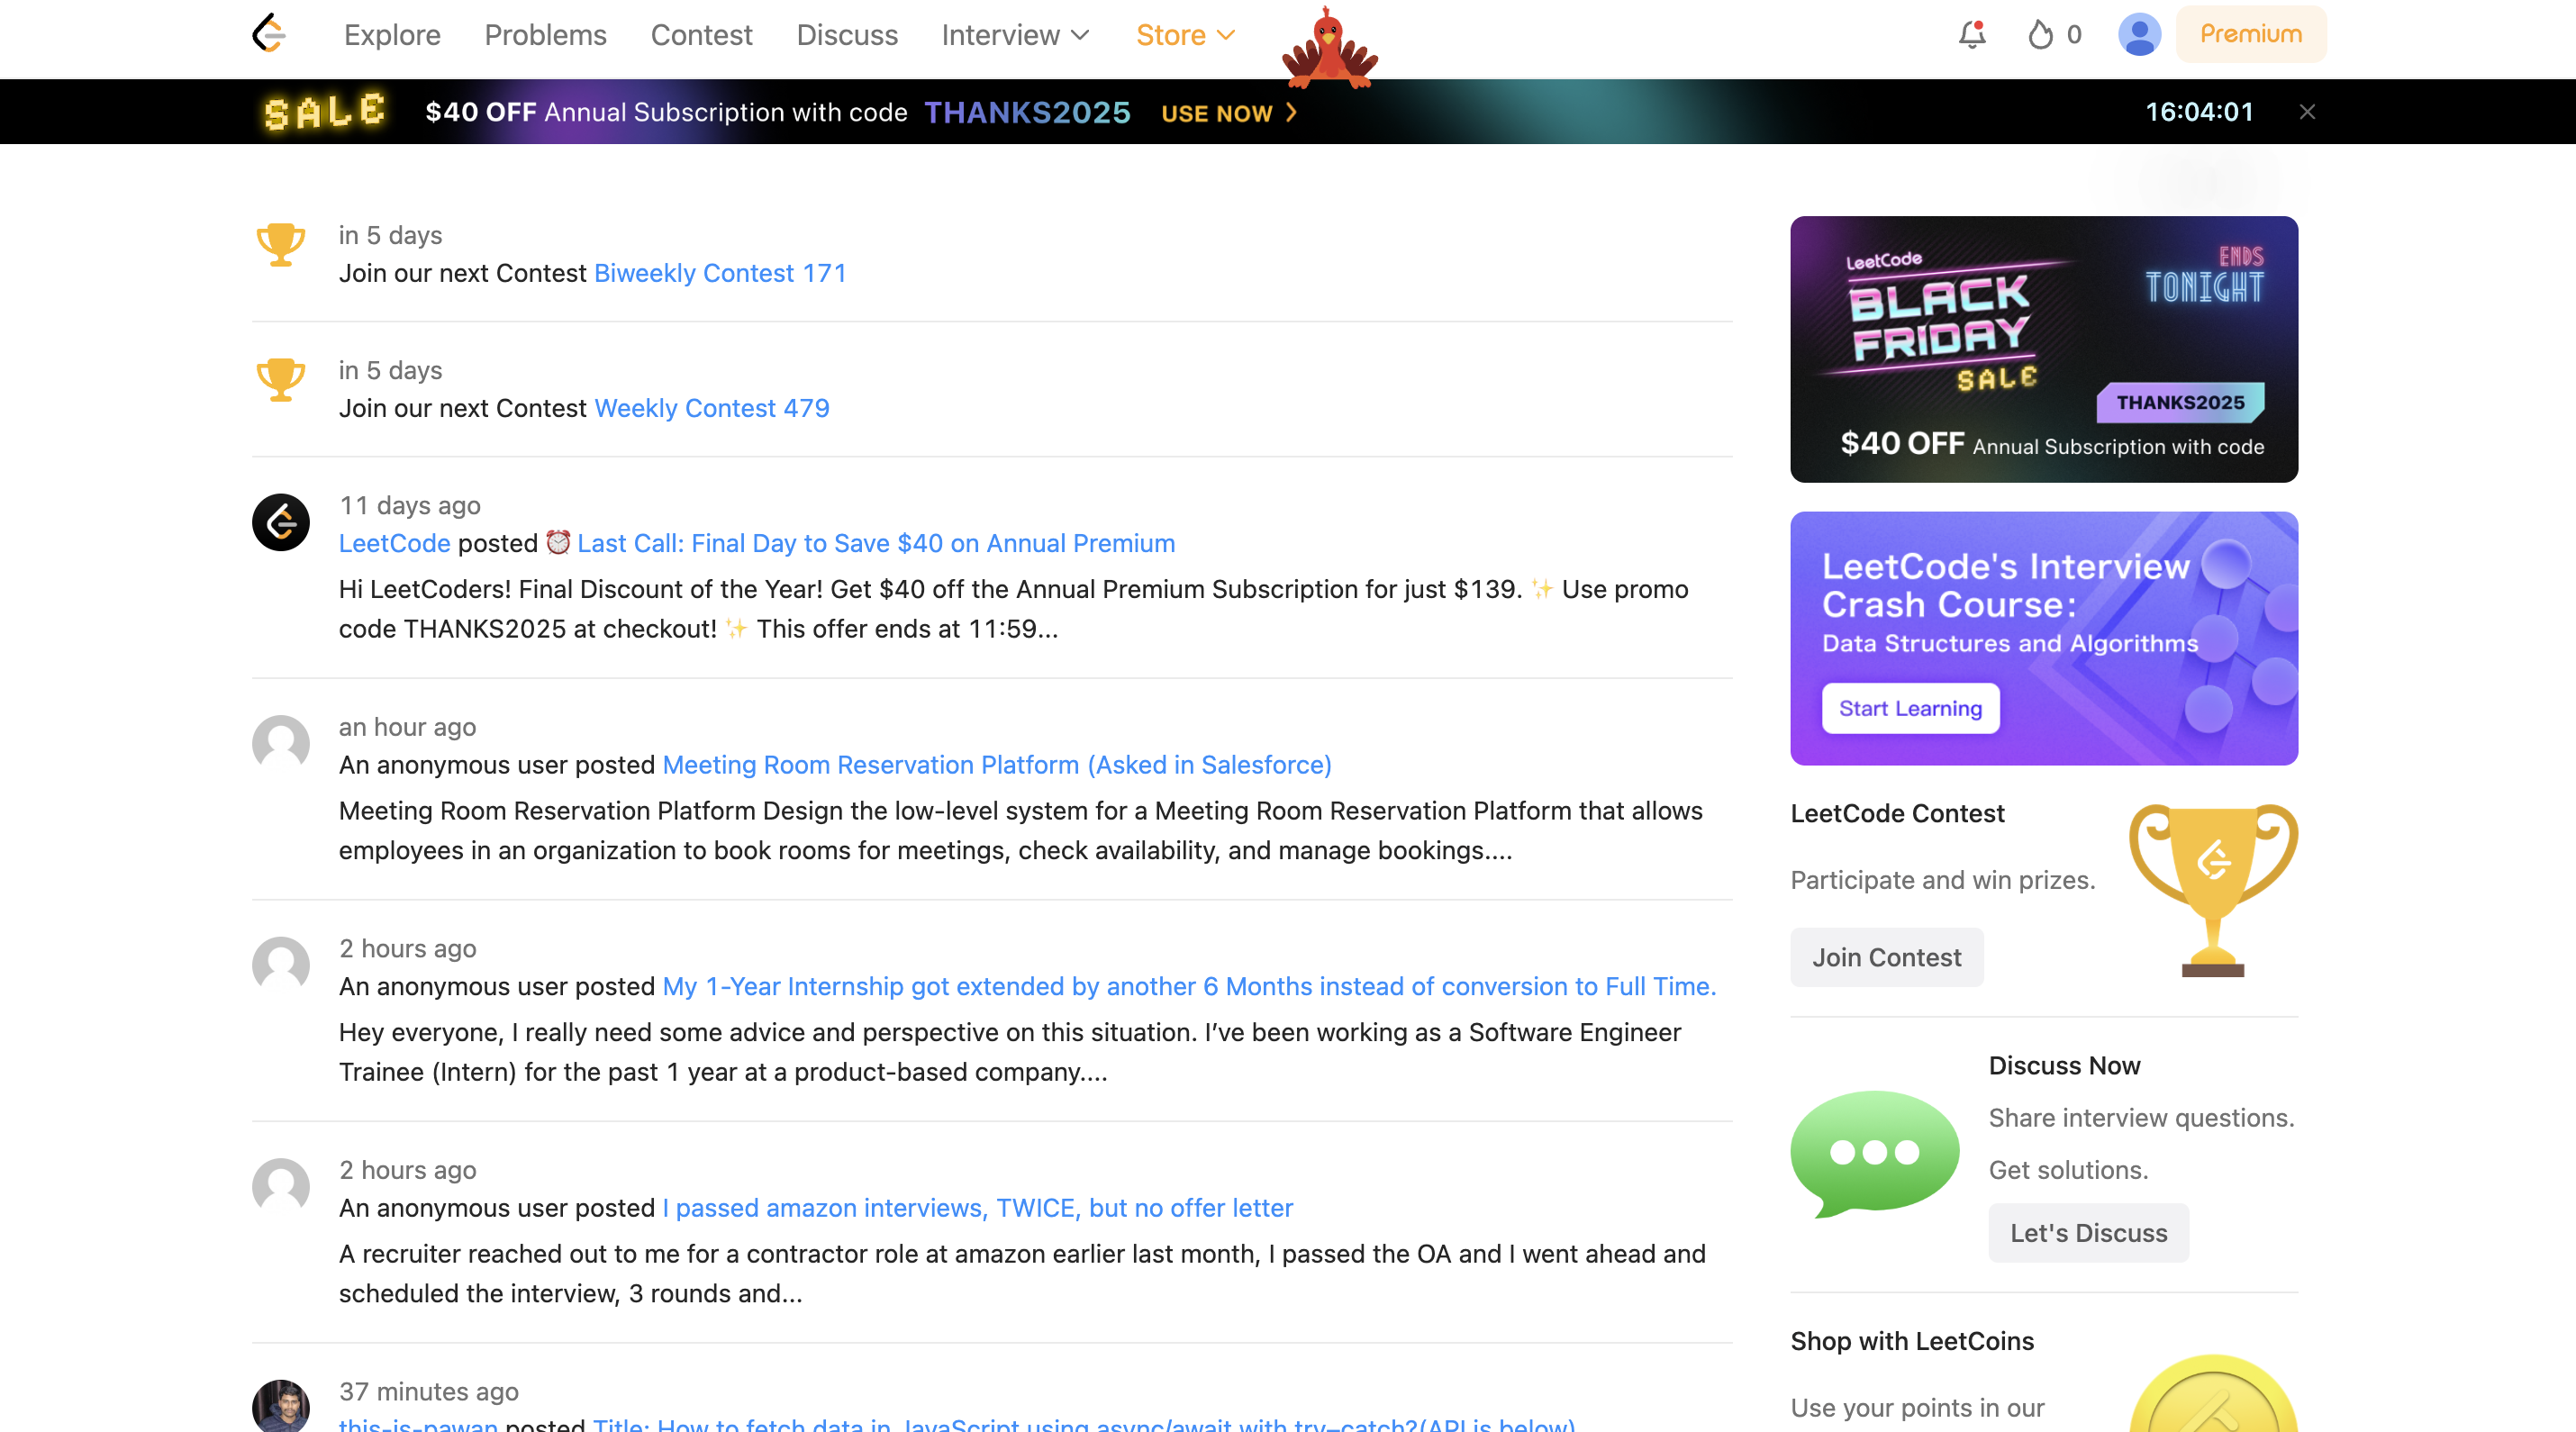
\includegraphics[width=1\textwidth]{Contents/Chapter 1/Images/Leetcode.png}
    \vspace{0.6cm}
    \caption{Leetcode Homepage}
    \label{fig:leetcode-system}
\end{figure}

LeetCode, founded in 2015 based on the co-founders’ experiences working at Google and Amazon, has become a highly popular online coding platform that offers a large collection of programming problems for all skill levels. It offers a comprehensive environment where users can practice a wide variety of programming problems, engage with a global community, and track their progress over time.LeetCode is widely recognized for its role in fostering problem-solving abilities and strengthening algorithmic thinking, making it an essential tool for both students and professionals in the software engineering field.\\

Key features of LeetCode include:
\begin{itemize}
    \item \textbf{Extensive Problem Library:} Thousands of coding problems across multiple difficulty levels and topics.
    \item \textbf{Online Code Editor:} Supports multiple programming languages with instant feedback and test case evaluation.
    \item \textbf{Contest and Challenge System:} Regular coding contests to benchmark skills against a global community.
    \item \textbf{Interview Preparation Kits:} Curated problem sets designed to prepare users for technical interviews at top tech companies.
    \item \textbf{Discussion Forums:} Active community discussions for problem-solving strategies, solutions, and learning resources.
    \item \textbf{Progress Tracking and Analytics:} Tools to monitor performance, problem-solving patterns, and skill improvement over time.
\end{itemize}

LeetCode offers a diverse set of core features that comprehensively address the needs of different user roles, including problem solving, submission tracking, contest participation, community interaction, ranking, and interview preparation. These features collectively enhance the learning experience, promote skill development, and encourage active engagement within the platform. However, it is noteworthy that LeetCode currently does not provide a public leaderboard to foster a stronger competitive environment among users.
\subsection{Codeforces}

\begin{figure}[h!]
    \centering
    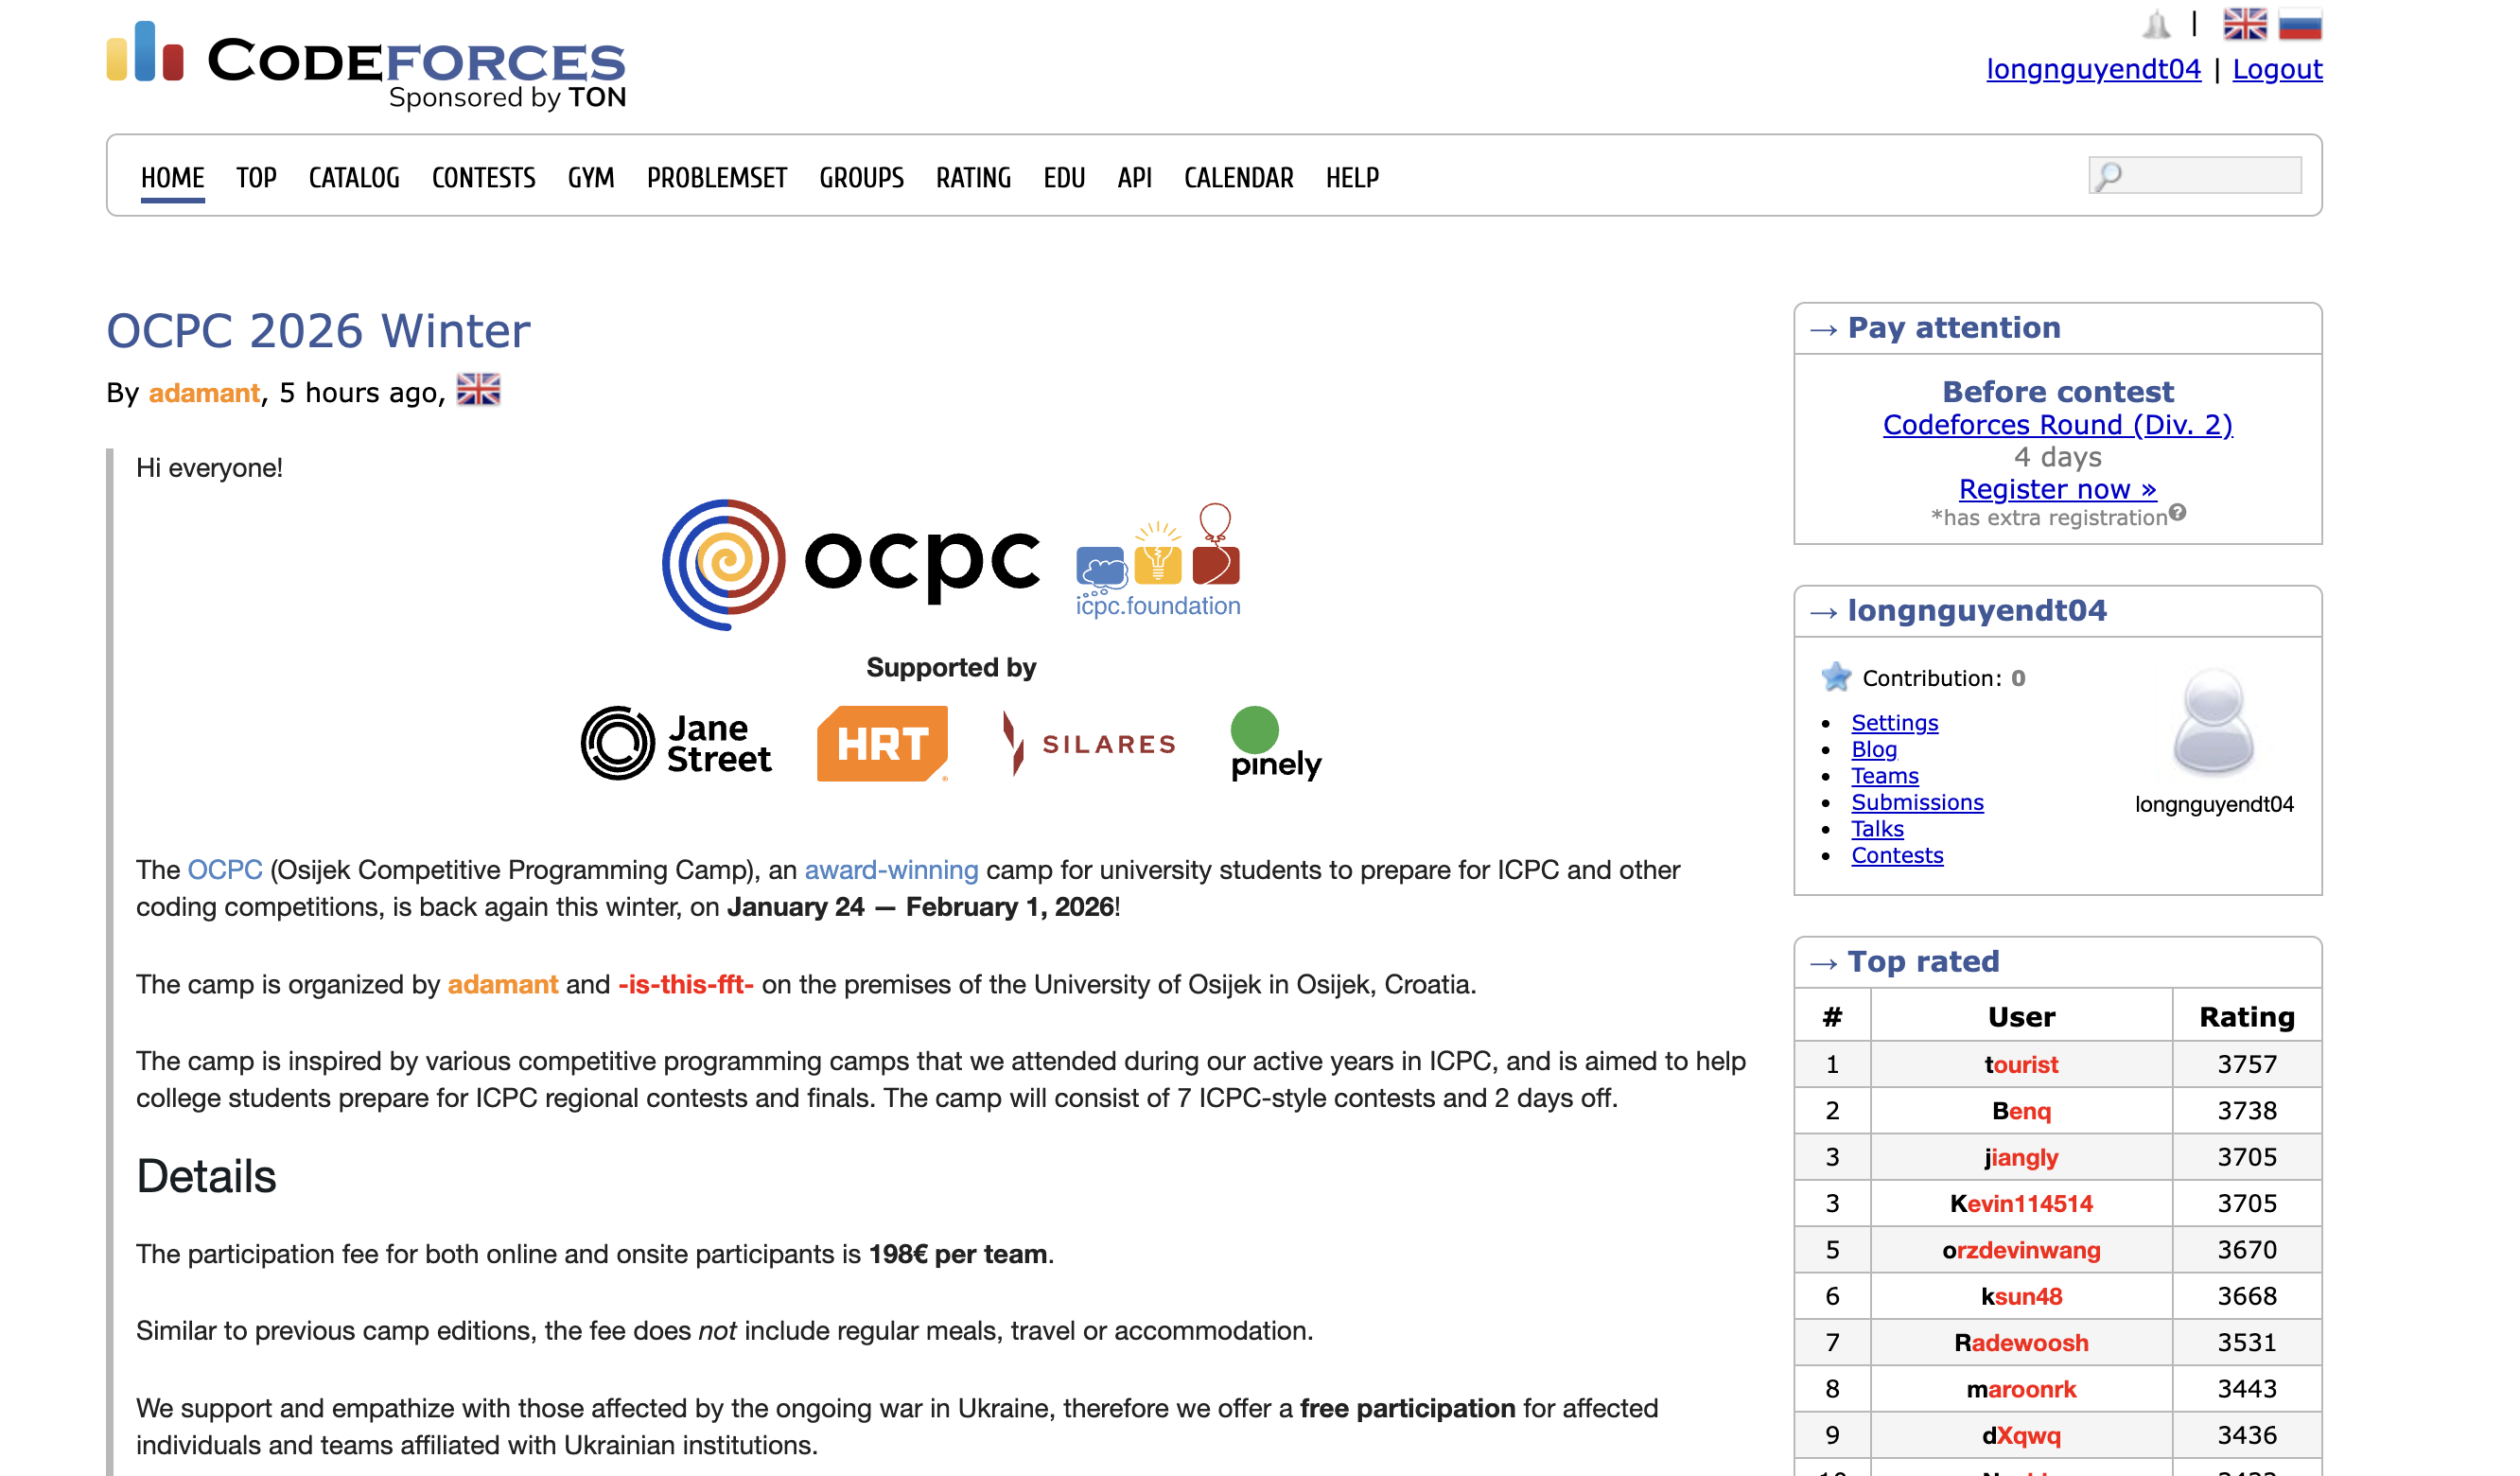
\includegraphics[width=1\textwidth]{Contents/Chapter 1/Images/Codeforces.png}
    \vspace{0.6cm}
    \caption{Codeforces Homepage}
    \label{fig:codeforces-system}
\end{figure}

Codeforces is a prominent online platform dedicated to competitive programming, offering users a structured environment to enhance their algorithmic and problem-solving skills through real-time contests. It is widely used by students, professionals, and competitive programmers to benchmark their abilities and engage with a global community of coders.\\

Key features of Codeforces include:
\begin{itemize}
    \item \textbf{Extensive Problem Sets:} A vast collection of algorithmic and programming problems across multiple difficulty levels.
    \item \textbf{Online Contests:} Regular timed competitions, including rated contests, that simulate real-world competitive programming scenarios.
    \item \textbf{Integrated Code Editor:} Supports multiple programming languages with submission, testing, and evaluation against problem test cases.
    \item \textbf{Community Discussion:} Active forums for problem discussions, solution sharing, and peer feedback.
    \item \textbf{User Ratings and Rankings:} Automatic rating system reflecting performance in contests and overall ranking among users globally.
    \item \textbf{Problem Tags and Difficulty Filters:} Tools to browse and search problems efficiently based on difficulty, topic, and tags.
\end{itemize}

Codeforces excels in providing a practical, competition-oriented environment that strengthens real-world programming and algorithmic skills. Its focus on timed contests and rigorous problem solving makes it an excellent platform for users aiming to improve performance in competitive programming. However, Codeforces does not currently provide dedicated tools for technical interview preparation, such as virtual assistants, hints, or structured interview question sets.

\subsection{VNOI Online Judge}

\begin{figure}[h!]
    \centering
    
\includegraphics[width=1\textwidth]{Contents/Chapter 1/Images/VNOI.png}
    \vspace{0.6cm}
    \caption{VNOI Online Judge Homepage}
    \label{fig:vnoi-system}
\end{figure}

VNOI Online Judge (VNOJ) is the official online judge system of the Vietnam Olympiad in Informatics community. The platform is based on the open-source DMOJ system and was built to provide a dedicated environment for Vietnamese learners to practice programming, compete in contests, and access problem sets from national and international competitions. VNOJ also continues the role of the former VOJ system by preserving and expanding a large archive of Vietnamese competitive programming problems.\\

Key features of VNOI Online Judge include:
\begin{itemize}
    \item \textbf{Vietnamese Problem Archive:} A large collection of problems from Vietnamese contests, national excellent student exams, ACM-ICPC style contests, and VNOI official events.
    \item \textbf{Automatic Online Judge:} Submission evaluation with verdicts, execution limits, and support for competitive programming workflows.
    \item \textbf{Contest System:} Official and practice contests organized for the Vietnamese competitive programming community.
    \item \textbf{User Ranking:} Public user profiles and ranking information that encourage competition and long-term practice.
    \item \textbf{Community Knowledge Base:} Links to VNOI Wiki, blogs, news, and learning resources focused on algorithms and programming contests.
    \item \textbf{Vietnamese Community Focus:} Content, announcements, and educational activities are tailored to Vietnamese students and competitive programmers.
\end{itemize}

VNOI Online Judge is especially valuable for Vietnamese IT students because it provides localized content, familiar contest formats, and access to problem sets from domestic competitions. Its strengths are closely aligned with competitive programming education and community development in Vietnam. However, VNOJ focuses mainly on algorithm practice and contest participation, while CodeRank aims to combine these competitive features with broader learning support such as interview preparation, centralized real-time discussions, and customizable user-created contests.

\subsection{ Websites comparison}
\begin{table}[h!]
\centering
\renewcommand{\arraystretch}{1.3}
\caption{Comparison of existing website with CodeRank}
\label{tab:website-comparison}
\begin{tabularx}{\textwidth}{|l|X|X|X|X|}
\hline
\textbf{Criteria} & \textbf{LeetCode} & \textbf{Codeforces} & \textbf{VNOI Online Judge} & \textbf{CodeRank} \\
\hline
Problem Library & Yes & Yes & Yes & Yes \\
\hline
Online Coding Editor & Yes & Yes & Yes & Yes \\
\hline
Community & Active discussion forums & Active forums with contest discussions & Vietnamese competitive programming community, blogs, wiki, and announcements & Centralized real-time discussion forums \\
\hline
Contest System & Regular contests organized by platform & Timed contests with system-created schedule & Official and practice contests for the VNOI community & Both official and user-created contests, customizable by users. \\
\hline
Interview Preparation & Yes & No & No & Yes \\
\hline
Ranking System & Points for solved problems, but not visible to all users & Rating system based on contest performance & Public user rankings and contest standings & Dynamic points for problem solving and public centralized leaderboard \\
\hline
Multilingual & Support English \& Chinese & Support English \& Russian & Mainly Vietnamese with some English problem content & Support English \& Vietnamese \\
\hline
\end{tabularx}
\end{table}

\FloatBarrier

Obviously, each platform has its own strengths: LeetCode offers an extensive problem library and dedicated interview preparation resources, Codeforces emphasizes timed contests, rating systems, and community-driven forums for competitive practice, and VNOI Online Judge provides localized Vietnamese problem sets, contests, and learning resources for the national competitive programming community. However, CodeRank combines these advantages and adds key enhancements, including both official and user-created contests with customizable settings, a centralized public leaderboard, real-time discussion forums, and multilingual support (including Vietnamese). These features make CodeRank a comprehensive, user-centered platform tailored to the educational and practical needs of Vietnamese IT students.

\newpage

\chapter {Technology Stack}
\noindent
\rule{\textwidth}{0.4pt}

\begin{center}
\begin{minipage}{0.8\textwidth}
\textit{The purpose of Chapter 2 is to provide a comprehensive technical overview and rationale behind the selection of the platform's diverse technology stack. The authors articulate the specifics of the chosen front-end and back-end frameworks, the database management system, the sandboxed execution environment tools, and the integration of the LLM model to facilitate the conversational chatbot feature.}
\end{minipage}
\end{center}

\section{Web Application Development}

\subsection*{Web Application Development}

The rapid evolution of technology has significantly increased the demand for web applications across various industries. A web application is a software program that is hosted on a remote server and delivered to users via the Internet. Unlike traditional desktop applications which is installed locally on a device, web applications are accessible through web browsers such as Google Chrome, Safari, Microsoft Edge, and others. Depending on the purpose and scale, web applications can range from simple tools, like a to-do list application, to a more complex and robust systems such as online coding platforms or enterprise resource management systems.\cite{lambdatest_web_application_developement}\\
\subsection*{Components of Web Applications}

Most web applications are composed of two primary components: frontend and backend.

\begin{enumerate}
    \item \textbf{Frontend Development}\\
    The frontend, also known as the client-side, refers to the part of the application that interacts directly with users. JavaScript is the predominant programming language for frontend development. At a basic level, developers use HTML, CSS, and JavaScript to build interactive pages. For applications at a larger scale, frameworks like AngularJS, ReactJS, or VueJS provide pre-built components and structured architectures, enabling scalable and dynamic user interfaces.

    \item \textbf{Backend Development}\\
    The backend, or server-side, handles business logic, database operations, authentication, and server communication. Popular technologies for backend development include Node.js, ASP.NET, Golang, Python (with Django or Flask), and Ruby on Rails. The backend is responsible for processing client requests, interacting with databases, and returning responses to the frontend.
\end{enumerate}

\vspace{1.5em}
\subsection*{Rendering Approaches}

Rendering is a crucial aspect of web application development, determining how content is delivered and displayed to users. There are two primary rendering strategies: Client-Side Rendering (CSR) and Server-Side Rendering (SSR).

In CSR, the server sends a minimal HTML document along with JavaScript bundles. The JavaScript executes in the browser to render the user interface dynamically. While CSR enables highly interactive applications and enhances user experience, it may introduce a slight delay during the initial page load, resulting in a temporary empty page. Moreover, CSR is less favorable for search engine optimization (SEO), as crawlers may not immediately access the fully rendered content.\cite{client_side_vs_server_side}

In SSR, the server generates a complete HTML page before sending it to the client. This allows browsers to display fully rendered pages immediately, improving the initial user experience and SEO performance. Pre-rendered HTML is easier for search engines like Google or Bing to crawl and index, which can positively affect the website’s ranking in search results.\cite{client_side_vs_server_side}

\section{Frontend Development}

Frontend development, also known as client-side development, focuses on creating the part of a web application that users directly interact with. It encompasses the design, layout, and interactivity of web pages, ensuring a responsive and user-friendly experience across different devices and browsers. Modern frontend development relies heavily on JavaScript as the primary programming language, complemented by HTML and CSS for structuring and styling content. Additionally, powerful frameworks and libraries such as ReactJS, AngularJS, and VueJS provide structured architectures, reusable components, and advanced features that enable developers to build dynamic, maintainable, and scalable user interfaces.

\subsection{AngularJS}

AngularJS is a widely used open-source JavaScript framework developed by Google, primarily designed to build dynamic and single-page web applications (SPAs). Unlike traditional web development, AngularJS allows developers to extend HTML syntax and implement rich client-side functionality in a structured and maintainable way.\cite{angularJS}

One of the key strengths of AngularJS is its two-way data binding, which synchronizes the model (JavaScript objects) and the view (HTML) automatically. This reduces the amount of boilerplate code required for updating the user interface and ensures that changes in the data are immediately reflected in the view, and vice versa.

AngularJS also employs a Model-View-Controller (MVC) architecture, separating the application into three interconnected components:
\begin{itemize}
    \item \textbf{Model}: Represents the application data and business logic.
    \item \textbf{View}: Defines the presentation layer and user interface.
    \item \textbf{Controller}: Acts as an intermediary between the Model and View, handling user input and manipulating the model accordingly.
\end{itemize}

Additional key technologies and features in AngularJS include:
\begin{enumerate}
    \item \textbf{Dependency Injection}: A design pattern that facilitates modularity, testability, and easier management of components.
    \item \textbf{Services}: Singleton objects or functions used to organize and share code across the application.
    \item \textbf{Routing and Navigation}: Built-in support for client-side navigation between different views without reloading the entire page.
    \item \textbf{Directives}: Custom HTML attributes and elements that extend HTML functionality, enabling reusable components.
\end{enumerate}

Overall, AngularJS provides a comprehensive framework for building scalable, maintainable, and highly interactive web applications, making it a preferred choice for many modern frontend development projects.

\subsection{ReactJS}

ReactJS is a widely adopted open-source JavaScript library developed by Facebook, primarily used for building dynamic and high-performance user interfaces, especially for single-page applications (SPAs). React focuses on the view layer and provides a component-based architecture that promotes modularity and reusability.\cite{ReactJS}

Key technologies and concepts in ReactJS include:
\begin{enumerate}
    \item \textbf{Components}: Reusable building blocks that encapsulate both UI and behavior, enabling modular development.
    \item \textbf{JSX (JavaScript XML)}: Allows HTML-like syntax within JavaScript for clearer and more maintainable code.
    \item \textbf{Virtual DOM}: Optimizes rendering performance by updating only the necessary parts of the actual DOM.
    \item \textbf{State and Props}: Manage component data (state) and pass data between components (props) with a unidirectional data flow.
    \item \textbf{Hooks}: Hooks allow functional components to use state and other React features without writing class components. 
\end{enumerate}

ReactJS provides a flexible and efficient approach to building interactive web applications, making it one of the most popular choices in modern frontend development.

\subsection{VueJS}

VueJS is an open-source JavaScript framework designed for building user interfaces and single-page applications (SPAs). It emphasizes a progressive approach, allowing developers to adopt its features incrementally, from enhancing existing HTML pages to developing complex applications. VueJS provides a reactive and component-based architecture that promotes modularity, maintainability, and efficient rendering.\cite{VueJS}

Key technologies and concepts in VueJS include:
\begin{enumerate}
    \item \textbf{Reactive Data Binding}: Automatically synchronizes the data model and the view, ensuring efficient updates and reducing boilerplate code.
    \item \textbf{Components}: Reusable building blocks that encapsulate structure, behavior, and styles, enabling modular development.
    \item \textbf{Directives}: Special HTML attributes that provide dynamic behavior and allow developers to extend HTML functionality.
    \item \textbf{Vue Router}: A powerful routing library that facilitates client-side navigation and enables the creation of single-page applications with multiple views.
    \item \textbf{Vuex}: A state management library for VueJS applications, providing a centralized store for managing application state in a predictable manner.
\end{enumerate}

VueJS provides a flexible, performant, and approachable framework for building modern web applications, making it a popular choice among frontend developers.

\subsection{Pros and Cons}

\clearpage

\begin{longtable}{|l|p{6cm}|p{6cm}|}
\caption{Frontend Technology Pros and Cons} \\
\hline
\textbf{Technology} & \textbf{Pros} & \textbf{Cons} \\
\hline

\textbf{AngularJS} &
\begin{minipage}[t]{\linewidth}
\begin{itemize}[leftmargin=*,noitemsep,nolistsep]
    \item Full-featured framework with built-in routing, dependency injection, and form handling.
    \item Strong typing with TypeScript improves code maintainability.
    \item Two-way data binding simplifies UI updates.
\end{itemize}
\end{minipage} &
\begin{minipage}[t]{\linewidth}
\begin{itemize}[leftmargin=*,noitemsep,nolistsep]
    \item Steeper learning curve due to complex concepts and TypeScript requirement.
    \item Verbose syntax and larger bundle size can affect performance.
\end{itemize}
\end{minipage} \\
\hline

\textbf{ReactJS} & 
\begin{minipage}[t]{\linewidth}
\begin{itemize}[leftmargin=*,noitemsep,nolistsep]
    \item Component-based architecture promotes modularity and reusability.
    \item Virtual DOM improves rendering performance.
    \item Large ecosystem and community support.
    \item Easy integration with other libraries and existing projects.
\end{itemize}
\end{minipage} &
\begin{minipage}[t]{\linewidth}
\begin{itemize}[leftmargin=*,noitemsep,nolistsep]
    \item Only handles the view layer, requires additional libraries for full MVC structure.
    \item Learning curve for state management libraries like Redux.
\end{itemize}
\end{minipage} \\
\hline

\textbf{VueJS} &
\begin{minipage}[t]{\linewidth}
\begin{itemize}[leftmargin=*,noitemsep,nolistsep]
    \item Lightweight and flexible framework.
    \item Easy to learn and integrate into existing projects.
    \item Reactive data binding and component-based architecture.
    \item Clear and concise syntax.
\end{itemize}
\end{minipage} &
\begin{minipage}[t]{\linewidth}
\begin{itemize}[leftmargin=*,noitemsep,nolistsep]
    \item Smaller ecosystem and fewer enterprise-scale resources compared to React or Angular.
    \item Community-driven plugins may vary in quality.
\end{itemize}
\end{minipage} \\
\hline

\end{longtable}

\FloatBarrier

In the context of CodeRank, ReactJS was selected as the frontend framework primarily because it provides a balanced combination of performance, flexibility, and a mature ecosystem. While AngularJS offers a comprehensive framework with built-in features such as routing, dependency injection, and two-way data binding, it comes with a steeper learning curve, verbose syntax, and larger bundle sizes, which can impact development speed and performance for the Coderank online platform. On the other hand, VueJS is lightweight and easy to learn, but its smaller ecosystem and limited enterprise-scale resources could pose challenges for long-term scalability and integration with third-party libraries. ReactJS, with its component-based architecture, Virtual DOM optimization, and extensive community support, enables modular, maintainable, and high-performance development. Moreover, React is one of the leading frontend technologies with a vast and active community, providing a wide range of tools, libraries, and resources that facilitate rapid development, integration, and problem-solving. Its flexibility and robust ecosystem make ReactJS the most suitable choice for building a dynamic, interactive, and scalable web application in this project.

\section{Backend Development}

Backend development, or server-side development, involves the implementation of business logic, data processing, and communication between the client and the server. It is responsible for handling database operations, authentication, authorization, and the overall functionality of the application behind the scenes. Backend frameworks such as NestJS, Spring Boot, and ASP.NET Core provide structured and scalable solutions, offering modular architectures, dependency injection, and extensive integration with databases and third-party services. By leveraging these frameworks, developers can create high-performance, maintainable, and enterprise-grade applications capable of supporting complex business requirements and large user bases.

\subsection{ASP.NET Core}

ASP.NET Core is a modern, open-source, and cross-platform web framework developed by Microsoft for building high-performance, secure, and scalable server-side applications. Running on the .NET runtime, ASP.NET Core provides a unified platform for developing web APIs, MVC applications, and microservices with consistent architecture and tooling. It emphasizes modularity, flexibility, and maintainability, allowing developers to structure large-scale applications efficiently.\cite{asp_net}

ASP.NET Core includes an integrated dependency injection system, middleware pipeline for request handling, and a comprehensive set of libraries for authentication, authorization, and security. It supports multiple architectural patterns, including MVC, Razor Pages, and minimal APIs, enabling developers to choose the most suitable approach for their project requirements. With built-in support for Entity Framework Core, ASP.NET Core simplifies database interactions and object-relational mapping, while its cross-platform capabilities ensure applications can be deployed on Windows, Linux, or macOS environments.  

Additionally, ASP.NET Core facilitates the development of microservices and cloud-native applications, with seamless integration to modern tools such as Docker, Kubernetes, and Azure services. Its extensive tooling ecosystem, combined with a large and active community, ensures rapid development, debugging, and deployment of enterprise-grade applications.

\subsection{NestJS}

NestJS is a progressive and extensible Node.js framework designed for building efficient, scalable, and maintainable server-side applications. It is developed with TypeScript and takes full advantage of modern JavaScript features, enabling developers to write clean, type-safe, and highly modular code. NestJS follows an opinionated architectural pattern inspired by Angular, incorporating concepts such as modules, controllers, services, and dependency injection, which promote separation of concerns and testable code. While Node.js provides the runtime environment and handles non-blocking, event-driven I/O operations, NestJS adds a structured framework that simplifies the development of enterprise-grade backend applications.\cite{nestJS}

Key features of NestJS include a modular architecture for organized and reusable code, a robust dependency injection system for managing service lifecycles, seamless integration with popular libraries such as TypeORM or Mongoose for database access, and compatibility with Express or Fastify as the underlying HTTP server. Furthermore, NestJS supports the development of microservices and real-time applications using WebSockets or gRPC, making it a versatile choice for projects requiring high performance, scalability, and maintainability.

\subsection{Spring Boot}

Spring Boot is a Java-based, open-source framework built on top of the Spring ecosystem, designed to simplify the creation of production-ready, stand-alone, and enterprise-grade server-side applications. Running on the Java Virtual Machine (JVM), Spring Boot abstracts complex configurations and provides a convention-over-configuration approach, enabling developers to focus on application logic rather than boilerplate setup.\cite{spring_boot}

It integrates seamlessly with the broader Spring ecosystem, including Spring Data for simplified database access, Spring Security for authentication and authorization, and Spring Cloud for building microservices with distributed configuration, service discovery, and fault tolerance. Spring Boot features an embedded server, such as Tomcat or Jetty, for easy deployment, and includes production-ready capabilities like health checks, metrics, and logging out-of-the-box.  

Key strengths of Spring Boot include its modular architecture, support for microservices, automatic dependency management, and extensive integration with enterprise-grade tools and libraries. These features make Spring Boot a robust and scalable framework for developing complex backend systems, RESTful APIs, and large-scale applications that require maintainability, high performance, and long-term support.

\subsection{Backend Technology Pros and Cons}

\clearpage 

\begin{longtable}{|l|p{6cm}|p{6cm}|}
\caption{Backend Technology Pros and Cons} \\
\hline
\textbf{Framework} & \textbf{Pros} & \textbf{Cons} \\
\hline

\textbf{ASP.NET Core} &
\begin{itemize}[leftmargin=*,noitemsep,nolistsep]
    \item High performance: Kestrel server ensures top-tier backend performance.
    \item Modern C\# language: Offers flexibility, modern features (LINQ, async/await, Record Types), and strong enterprise orientation.
    \item Cross-platform development: Fully open-source and runs on Windows, Linux, and macOS.
\end{itemize} &
\begin{itemize}[leftmargin=*,noitemsep,nolistsep]
    \item Legacy perception: Some still associate it with Windows-only or Microsoft-only ecosystem.
    \item External library ecosystem: Although improved, third-party libraries are less diverse than Java or Node.js ecosystems.
\end{itemize} \\
\hline

\textbf{NestJS} &
\begin{itemize}[leftmargin=*,noitemsep,nolistsep]
    \item Modern architecture: Applies well-established design patterns and principles (Dependency Injection, Modules), facilitating organized and maintainable code.
    \item TypeScript support: Provides static typing, allowing early error detection and better maintainability for large-scale projects.
    \item Rapid development: Integrated CLI streamlines project setup and accelerates development.
    \item High I/O performance: Non-blocking I/O model of Node.js suits real-time and I/O-intensive applications.
\end{itemize} &
\begin{itemize}[leftmargin=*,noitemsep,nolistsep]
    \item Node.js dependency: Single-threaded by default, which may be less efficient for CPU-intensive tasks.
    \item Enterprise maturity: Node.js ecosystem, while large, may have fewer enterprise-grade solutions compared to Java/Spring or .NET.
\end{itemize} \\
\hline

\textbf{Spring Boot} &
\begin{itemize}[leftmargin=*,noitemsep,nolistsep]
    \item Industry standard: Widely adopted for enterprise applications and microservices architecture.
    \item Mature ecosystem: Offers numerous modules (Spring Data, Spring Security, Spring Cloud) covering a wide range of backend needs.
    \item High performance and scalability: JVM with optimized garbage collection delivers strong CPU performance.
    \item Excellent support: Extensive documentation and community support for enterprise projects.
\end{itemize} &
\begin{itemize}[leftmargin=*,noitemsep,nolistsep]
    \item Slower startup: Traditional Spring Boot applications may have longer initialization times due to IoC container setup.
    \item Resource consumption: JVM-based applications generally require more RAM memory.
    \item Verbose syntax: Java code can be more verbose and less expressive than C\# or TypeScript.
\end{itemize} \\
\hline

\end{longtable}


In this project, NestJS was chosen as the backend framework primarily because it provides a structured and scalable architecture while leveraging the same language used in frontend development—JavaScript/TypeScript. This alignment allows the development team to maintain consistency across the full stack, reduce context switching, and promote code reusability. While Spring Boot and ASP.NET Core are mature frameworks with strong enterprise support, they require knowledge of Java and C\# respectively, which introduces additional complexity for a team primarily working with JavaScript. NestJS, with its modular design, built-in dependency injection, and seamless integration with the Node.js ecosystem, enables efficient development of high-performance, maintainable, and scalable server-side applications. Furthermore, NestJS supports microservices, WebSockets, and real-time features, making it a versatile choice for the dynamic and interactive requirements of the Coderank online platform.

\section{Database}

Databases are a critical component of web applications, providing a structured way to store, retrieve, and manage data. There are several types of databases used in web development, each with its own strengths and use cases.

\subsection{Relational Databases}

Relational databases, such as MySQL and PostgreSQL, organize data into tables with predefined schemas. They use Structured Query Language (SQL) for data manipulation and are known for their ACID (Atomicity, Consistency, Isolation, Durability) properties, ensuring reliable transactions. Relational databases are ideal for applications with complex queries and relationships between data entities.\\

\subsection*{MySQL}

MySQL is a widely adopted relational database management system known for its high performance, ease of use, and strong community support. It follows a traditional SQL-based approach and is optimized for read-heavy workloads, making it suitable for web applications, content management systems, and e-commerce platforms. MySQL provides efficient indexing, replication capabilities, and supports various storage engines—most notably InnoDB, which offers ACID compliance and foreign-key constraints. Although MySQL handles standard SQL operations effectively, it has more limited support for advanced features such as complex joins, window functions (in earlier versions), and full transactional consistency across certain operations.\cite{mysql} \\

\subsection*{PostgreSQL}

PostgreSQL is an advanced, open-source relational database system distinguished by its strong emphasis on standards compliance, extensibility, and robustness. It supports sophisticated SQL features, including window functions, common table expressions (CTEs), full-text search, and advanced indexing methods such as GiST and GIN. PostgreSQL is highly suitable for applications requiring complex queries, strict data integrity, and transactional reliability. Additionally, its extensible architecture allows developers to define custom data types, operators, and functions, making it a popular choice for enterprise systems, analytical workloads, and applications requiring both relational and semi-structured data handling (e.g., via its powerful JSONB support).\cite{postgresql}

\subsection{NoSQL Databases}

NoSQL databases, like MongoDB and Cassandra, offer a more flexible schema design, allowing for unstructured or semi-structured data storage. They are designed to scale horizontally, making them suitable for handling large volumes of data and high-velocity workloads. NoSQL databases are commonly used in applications requiring rapid development and iteration, such as content management systems and real-time analytics.\\

\subsection*{MongoDB}

MongoDB is a document-oriented NoSQL database that stores data in flexible JSON-like documents, allowing developers to handle unstructured and semi-structured data with ease. Its dynamic schema makes it highly suitable for agile development, where data models evolve frequently. MongoDB supports rich querying capabilities, indexing, aggregation pipelines, and geospatial operations, enabling both transactional and analytical use cases. Additionally, its built-in horizontal scaling through sharding allows the system to handle massive datasets and high read/write throughput efficiently. MongoDB is often preferred for applications such as content management platforms, user-generated content systems, mobile backends, and event-driven architectures.\cite{mongodb} \\

\subsection*{Cassandra}

Cassandra is a highly scalable, distributed NoSQL database designed for handling large volumes of data across multiple commodity servers. It employs a wide-column store model, allowing for flexible schema design and efficient storage of sparse data. Cassandra's architecture is built for high availability and fault tolerance, with no single point of failure, making it ideal for applications requiring continuous uptime and resilience. It uses a peer-to-peer distributed system and supports eventual consistency, which allows for high write throughput and low latency reads. Cassandra is particularly well-suited for use cases such as real-time analytics, IoT data management, recommendation engines, and large-scale messaging systems.\cite{cassandra}

\subsection{Database Technology Pros and Cons}

\newpage

\begin{longtable}{|p{3cm}|p{6cm}|p{6cm}|}
\caption{Database Technology Pros and Cons} \\
\hline
\textbf{Database} & \textbf{Pros} & \textbf{Cons} \\
\hline

MySQL &
\begin{itemize}[leftmargin=*,noitemsep,nolistsep]
  \item Very widely used, strong community \& ecosystem.
  \item High performance for read-heavy workloads.
  \item Mature, stable, easy to integrate with many platforms
  \item Free and open-source (core version).
\end{itemize}
&
\begin{itemize}[leftmargin=*,noitemsep,nolistsep]
  \item Limited advanced SQL features compared to PostgreSQL.
  \item Handles concurrent writes less efficiently.
  \item Not ideal for very complex queries.
\end{itemize}
\\ \hline

PostgreSQL &
\begin{itemize}[leftmargin=*,noitemsep,nolistsep]
  \item Full ACID compliance and advanced SQL features.
  \item Highly extensible (custom types, functions, etc.).
  \item Strong concurrency control for write-heavy applications.
  \item Fully open-source without proprietary licensing.
\end{itemize}
&
\begin{itemize}[leftmargin=*,noitemsep,nolistsep]
  \item Slightly slower for simple read-heavy workloads.
  \item More resource-intensive; requires tuning.
  \item More complex to set up and manage.
\end{itemize}
\\ \hline

MongoDB &
\begin{itemize}[leftmargin=*,noitemsep,nolistsep]
  \item Flexible schema; great for unstructured/semi-structured data.
  \item Horizontally scalable; built-in sharding.
  \item JSON-like documents (developer-friendly).
  \item High performance for real-time apps \& analytics.
\end{itemize}
&
\begin{itemize}[leftmargin=*,noitemsep,nolistsep]
  \item Weaker ACID guarantees; multi-document transactions are limited.
  \item Easier to create inconsistent data if schema is not managed well.
  \item Memory-heavy for large datasets.
\end{itemize}
\\ \hline

Cassandra &
\begin{itemize}[leftmargin=*,noitemsep,nolistsep]
  \item Highly scalable for very large datasets.
  \item Designed for high availability and fault tolerance.
  \item Excellent write performance for heavy workloads.
  \item Supports flexible schema with column-family model.
  \item Distributed architecture with no single point of failure.
\end{itemize}
&
\begin{itemize}[leftmargin=*,noitemsep,nolistsep]
  \item Not fully ACID compliant; eventual consistency model.
  \item Complex to query compared to SQL databases.
  \item Limited support for joins and aggregations.
  \item Requires careful schema design for performance.
\end{itemize}
\\ \hline

\end{longtable}

Based on the comparison of popular database systems, PostgreSQL was chosen for the CodeRank project due to its strong support for ACID-compliant transactions and advanced SQL features, ensuring data consistency and integrity across user records, scores, and activity history. Its high extensibility, including support for custom data types and functions, allows the implementation of complex logic such as ranking algorithms and analytics. Additionally, PostgreSQL offers robust concurrency control, making it well-suited for our online coding platform with multiple simultaneous users. Although it requires more resources and careful configuration than simpler databases, PostgreSQL is stable with multiple useful features, which makes it an optimal choice for building database for CodeRank that can grow and stay reliable.
\section{Sandboxed Execution Environment}
In the world of cybersecurity, a \textbf{sandbox environment} is an isolated virtual machine in which potentially unsafe software code can execute without affecting network resources or local applications. Think of a sandbox as a controlled playground where applications, code, and files can be tested or executed to see how they behave. If the software behaves maliciously or unexpectedly, it doesn’t have the power to affect anything outside of that contained environment. \cite{proofpoint_sandbox}

In the context of CodeRank System, this mechanism is essential because the platform allows users to submit arbitrary source code for compilation and execution as part of algorithm practice and programming contests. Without sandboxing, user submissions could intentionally or accidentally access the file system, overload system resources, execute harmful commands, or interfere with other users’ submissions. By running each submission inside a sandbox, CodeRank ensures that all code is contained, resource-restricted, and prevented from performing dangerous operations. This guarantees fair evaluation, protects the platform’s infrastructure, and maintains a secure environment for all Vietnamese IT students using the system.

By considering the requirements for securely running user-submitted code, it is essential to evaluate different execution sandbox technologies used in modern online judge systems. In the following section, three representative tools will be introduced and compared in terms of security, performance, isolation level, and ease of integration.

\subsection{Firecracker MicroVMs}
Firecracker is an open source virtualization technology that is purpose-built for creating and managing secure, multi-tenant container and function-based services. Firecracker enables you to deploy workloads in lightweight virtual machines, called microVMs, which provide enhanced security and workload isolation over traditional VMs, while enabling the speed and resource efficiency of containers. Firecracker was developed at Amazon Web Services to improve the customer experience of services like AWS Lambda and AWS Fargate. \cite{firecracker2025}
\section{Artificial Intelligence}
\subsection{Gemini models from Google AI}
Gemini is Google’s family of state-of-the-art multimodal large language models designed to understand and generate text, code, and visual content with high efficiency. Gemini models are trained on diverse datasets and optimized for real-world applications such as software development, conversational agents, educational tools, and knowledge retrieval systems.  


\textbf{Key Concepts of Gemini for Software Development:}
\begin{itemize}
    \item \textbf{Multimodal Input Support:} Gemini accepts text, code, images, and other structured inputs, though CodeRank primarily utilizes its text and code understanding capabilities.
    \item \textbf{Tokens and Context Window:} Gemini processes input as tokens. Gemini 2.5 Flash offers an extended context window (up to 1 million tokens in some tiers), enabling long conversational history and detailed problem analysis.
    \item \textbf{Function Calling:} Gemini supports structured function calling, allowing developers to integrate model outputs into application logic, such as triggering code evaluation, retrieving problem metadata, or interacting with student performance data.
\end{itemize}

For the CodeRank system, we selected the \textbf{Gemini 2.5 Flash} model due to its strong performance on coding tasks and optimization for latency-sensitive applications. The model excels in:
\begin{itemize}
    \item Understanding programming questions and competitive programming prompts,
    \item Generating helpful explanations and hints for algorithm problems,
    \item Assisting users through conversational interactions within the platform’s chatbot,
    \item Performing reasoning tasks such as step-by-step code review or guidance on debugging.
\end{itemize}

Additionally, one significant advantage of Gemini 2.5 Flash is the availability of a \textbf{free-tier quota} in Google AI Studio, making it a highly cost-effective choice for our system. This enables the platform to deliver AI-powered features without incurring substantial operational expenses, which is especially valuable during development, prototyping, and early deployment stages. Furthermore, the free-tier support makes Gemini 2.5 Flash particularly suitable for building an MVP prototype and demonstrating a reliable proof of concept (POC) before scaling the solution.


\chapter {System Design and Analysis}
\noindent
\rule{\textwidth}{0.4pt}

\begin{center}
\begin{minipage}{0.8\textwidth}
\textit{Chapter 3 presents the system design and analysis of the CodeRank platform. It first defines the stakeholders, functional requirements, and non-functional requirements, followed by the major use cases of the system. The chapter then describes the architecture, submission evaluation flow, ranking mechanism, database schema, and chatbot design that support the platform's core functionality.}
\end{minipage}

\end{center}

\section{Requirement analysis}
\subsection{Stakeholders}
In any software system, understanding the stakeholders is essential for defining responsibilities, ensuring smooth operation, and aligning the platform with user needs. This project identifies three main groups of stakeholders, each playing a critical role in the development, management, and effective use of the platform. The following sections describe these groups in detail: Primary Users, Moderators, and Superadmin.
\begin{enumerate}
    \item \textbf{Primary Users}\\
    Primary users consist of students, programming contestants, and job seekers who utilize the platform to enhance their coding abilities and evaluate their technical proficiency. These users engage with the system by practicing programming challenges, submitting solutions for automated evaluation, and participating in online contests that allow them to monitor their progress and compare performance with peers. Additionally, they may take part in discussion forums to exchange ideas and seek guidance. The platform also provides access to an integrated virtual assistant designed to support interview preparation, enabling users to develop both competitive and career-readiness skills.
    \item \textbf{Moderators}\\
    Moderators serve as the quality control and management layer of the platform. Their responsibilities include reviewing problem statements, validating test cases, and monitoring ongoing contests to ensure fairness and a seamless experience for all participants. Moreover, moderators oversee the integrity of the system by detecting plagiarism, resolving disputes, and upholding community standards within discussion forums. Their involvement is essential for maintaining a trustworthy, transparent, and academically honest environment.
    \item \textbf{Superadmin}\\
    The Superadmin holds the highest level of authority within the system and is responsible for overarching platform management. In addition to performing all moderator functions, the Superadmin oversees system-wide operations, configures platform policies, and supervises both moderators and regular users. Their core duties include creating and managing moderator accounts, managing roles, addressing escalated issues, and monitoring system performance through analytics and operational metrics. This role ensures that the platform remains stable, secure, and aligned with organizational objectives.
\end{enumerate}

\subsection{Functional requirements}
\vspace{0.3cm}
\noindent \textbf{\Large Primary Users}
\vspace{0.3cm}
\begin{enumerate}[label=\arabic*.]
    \item \textit{Authentication:}
        \begin{itemize}
            \item The system shall allow users to create an account using email and password or third-party authentication providers (e.g., Google, GitHub).
            \item The system shall support secure login and logout functionality.
            \item The system shall provide password recovery and reset options.
            \item The system shall enforce role-based access control to differentiate between standard users, moderators, and superadmins.
        \end{itemize}
    \item \textit{Problem Solving and Submission:}
        \begin{itemize}
            \item The system shall allow users to browse and search algorithmic problems by difficulty, topic, tags, and status (solved, attempted).
            \item The system shall provide an integrated code editor supporting multiple programming languages (C++, Java, Python), enabling users to write, compile, and execute their code against provided example test cases.
            \item The system shall display immediate feedback on submitted solutions, indicating success/failure, execution time, memory usage, and specific error messages (e.g., Wrong Answer, Time Limit Exceeded, Runtime Error).
            \item The system shall allow users to view their past submissions and their results.
        \end{itemize}
    \item \textit{Contest Participation:}
        \begin{itemize}
            \item The system shall enable users to create or participate in online programming contests. In case the users want to create an online contest, they can enforce the contest rules, such as time limits per problem and penalty for incorrect submissions.
            \item The system shall display a leaderboard after the contests finish.
        \end{itemize}
    \item \textit{Community forum:}
        \begin{itemize}
            \item The system shall provide a shared discussion forum where users can exchange ideas, ask questions, and discuss solutions for all problems, similar to a general online community forum.
            \item The system shall allow users to upvote/downvote comments and report inappropriate content.
        \end{itemize}
    \item \textit{Ranking System:}
        \begin{itemize}
            \item The system shall assign points to users upon successfully solving problems, with points varying according to the difficulty of each problem.
            \item The ranking system shall update user scores and global rankings every 15 minutes, reflecting users’ latest achievements and progress.
        \end{itemize}
    \item \textit{Interview Preparation (Virtual Assistant):}
        \begin{itemize}
            \item The system shall offer a virtual assistant feature for practicing interview questions (e.g., mock interviews with predefined scenarios).
            \item The system shall provide hints and feedback on interview responses.
        \end{itemize}
\end{enumerate}
\vspace{0.3cm}
\noindent \textbf{\Large Moderators}
\vspace{0.3cm}
\begin{enumerate}
    \item \textit{Problems Management:}
        \begin{itemize}
            \item The system shall allow moderators to create, edit, and publish new algorithmic problems.
            \item The system shall enable moderators to define problem statements, input/output formats, constraints, and sample test cases.
            \item The system shall allow moderators to upload and manage hidden test cases for problem evaluation.
        \end{itemize}
    \item \textit{Contest Management:}
        \begin{itemize}
            \item The system shall allow moderators to receive and review requests from users for creating new contests. Moderators shall have the ability to either approve or reject these contest creation demands, providing a reason for rejection if applicable. Upon approval, the system shall notify the requesting user and enable the moderator to proceed with configuring and publishing the contest.
        \end{itemize}
    \item \textit{Community Moderation:}
        \begin{itemize}
            \item The system shall allow moderators to review and manage content in discussion forums, including deleting inappropriate posts or comments.
            \item The system shall enable moderators to warn or ban users who violate community guidelines.
        \end{itemize}
\end{enumerate}
\vspace{0.3cm}
\noindent \textbf{\Large Superadmin}
\vspace{0.3cm}\\
The Superadmin shall possess all the functional capabilities and permissions granted to a moderator.
\begin{enumerate}
    \item \textit{User and Moderator Account Management:}
        \begin{itemize}
            \item The system shall allow the Superadmin to create, edit, suspend, and delete user and moderator accounts.
            \item The system shall enable moderators to warn or ban users who violate community guidelines.
        \end{itemize}
\end{enumerate}

\subsection{Non-functional requirements}
\noindent \textit{Performance:} The system shall support at least 1,000 concurrent users while maintaining minimal latency during contests. Code submissions must be evaluated and feedback returned within 3 seconds for standard test cases, ensuring a responsive and smooth user experience.\\

\noindent \textit{Scalability:} The system shall be designed to support horizontal scaling, allowing it to handle increasing numbers of users and higher workloads by adding additional servers or computational resources as needed.\\

\noindent \textit{Reliability:} The system shall maintain high availability, particularly during contests and peak usage periods. Mechanisms for fault tolerance and recovery shall be implemented to minimize downtime and ensure continuous operation.\\

\noindent \textit{Security:} The system shall safeguard user accounts, code submissions, and any sensitive data (including payment information) through industry-standard security measures, such as encryption, secure authentication, and role-based access control.\\

\noindent \textit{Usability:} The system shall provide an intuitive and user-friendly interface suitable for both beginners and advanced users. Users should be able to quickly locate problems by difficulty or topic, join contests with minimal steps, and utilize the integrated code editor without additional setup.\\

\noindent \textit{Maintainability:} The system shall be designed for ease of maintenance, allowing developers to update features, fix bugs, and enhance functionality with minimal effort and disruption.\\

\noindent \textit{Internationalization \& Localization:} The system shall support multiple languages and provide seamless switching between them, ensuring accessibility and usability for a diverse, global user base.
\section{Use Cases}
\subsection{General Use Case}

\begin{figure}[h!]
    \centering
    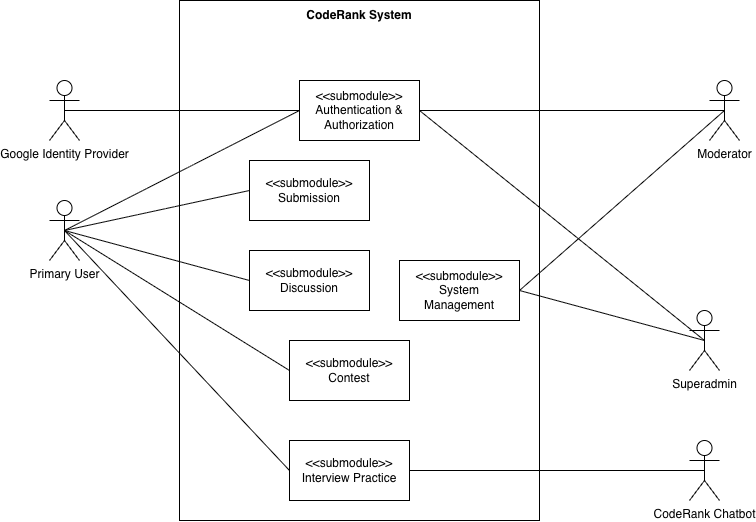
\includegraphics[width=1\textwidth]{Contents/Chapter 3/Usecase/Images/GeneralUsecase.png}
    \vspace{0.6cm}
    \caption{General Use Case}
\end{figure}


Our system contains 5 main submodules:
\begin{itemize}
    \item \textbf{Authentication \& Authorization}: Responsible for managing secure login and enforces Role-Based Access Control for 3 types of user.
    \item \textbf{Discussion}: Facilitates community interaction, allowing primary users to share solutions and ask questions related to problems. 
    \item \textbf{System Management}: The administrative interface used by Moderator and Superadmin to manage the problem creation, test cases, contests management and global user accounts.
Contest: Enables timed, high-stakes programming events with real-time ranking and automated leaderboards.
    \item \textbf{Submission}: This core module handles the presentation of the coding challenge and the automatic evaluation of the user's submitted solution.
\end{itemize}

\subsection{Use-case diagrams for each submodule}

\begin{figure}[h!]
    \centering
    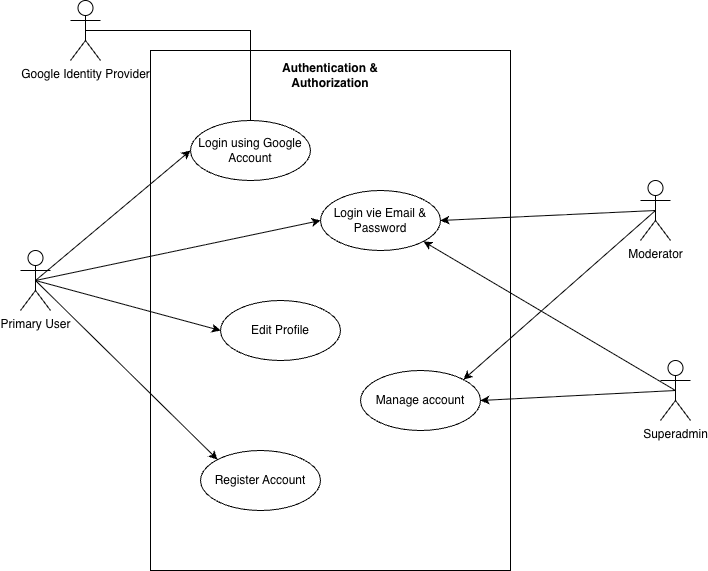
\includegraphics[width=1\textwidth]{Contents/Chapter 3/Usecase/Images/GeneralUsecase-Authentication.drawio.png}
    \vspace{0.6cm}
    \caption{Authentication \& Authorization Use Case}
\end{figure}
This submodule serves as the primary security gate for the entire system. Its core responsibility is to handle all user authentication (logging in) and authorization (managing access rights). This is crucial for protecting users' personal information, ensuring data privacy, and securing sensitive actions within the platform. By strictly controlling access, the module prevents unauthorized entry and maintains system integrity.
For user convenience, we offer diverse login methods:
\begin{itemize}
    \item Primary Users can log in quickly using their Google Account or use the traditional \textbf{Email \& Password} method.
    \item However, for privileged administrative roles—the Moderator and the Superadmin—access is strictly limited to the Login via \textbf{Email \& Password} method to enforce heightened security and traceability for system management functions.
\end{itemize}

All users retain standard account management capabilities, including registering a new account and changing their password.

\begin{figure}[h!]
    \centering
    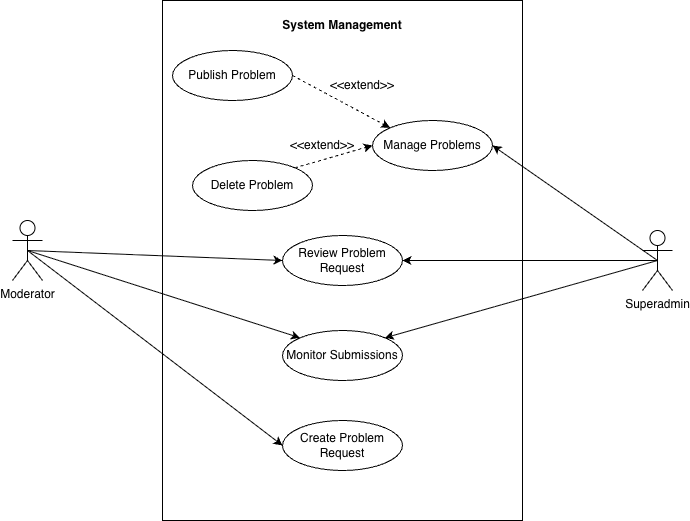
\includegraphics[width=1\textwidth]{Contents/Chapter 3/Usecase/Images/GeneralUsecase-SystemManagement.drawio.png}
    \vspace{0.6cm}
    \caption{System Management Use Case}
\end{figure}
The \textbf{System Management submodule} is the administrative dashboard used exclusively by the \textbf{Moderator} and \textbf{Superadmin} roles to control the content and operation of the platform.
\begin{itemize}
    \item \textbf{Problem Management}: Only Superadmin is enabled to manage problems directly (create, modify, delete) without reviewing steps
    \item \textbf{Content Workflow}: The Moderator initiates a Create Problem Request, and both the Moderator and Superadmin review problem requests before they go live.
    \item \textbf{Quality Control}: Both roles Monitor Submissions to track user activity, diagnose potential grading issues, and ensure fair play.
\end{itemize}
\clearpage

\begin{figure}[h!]
    \centering
    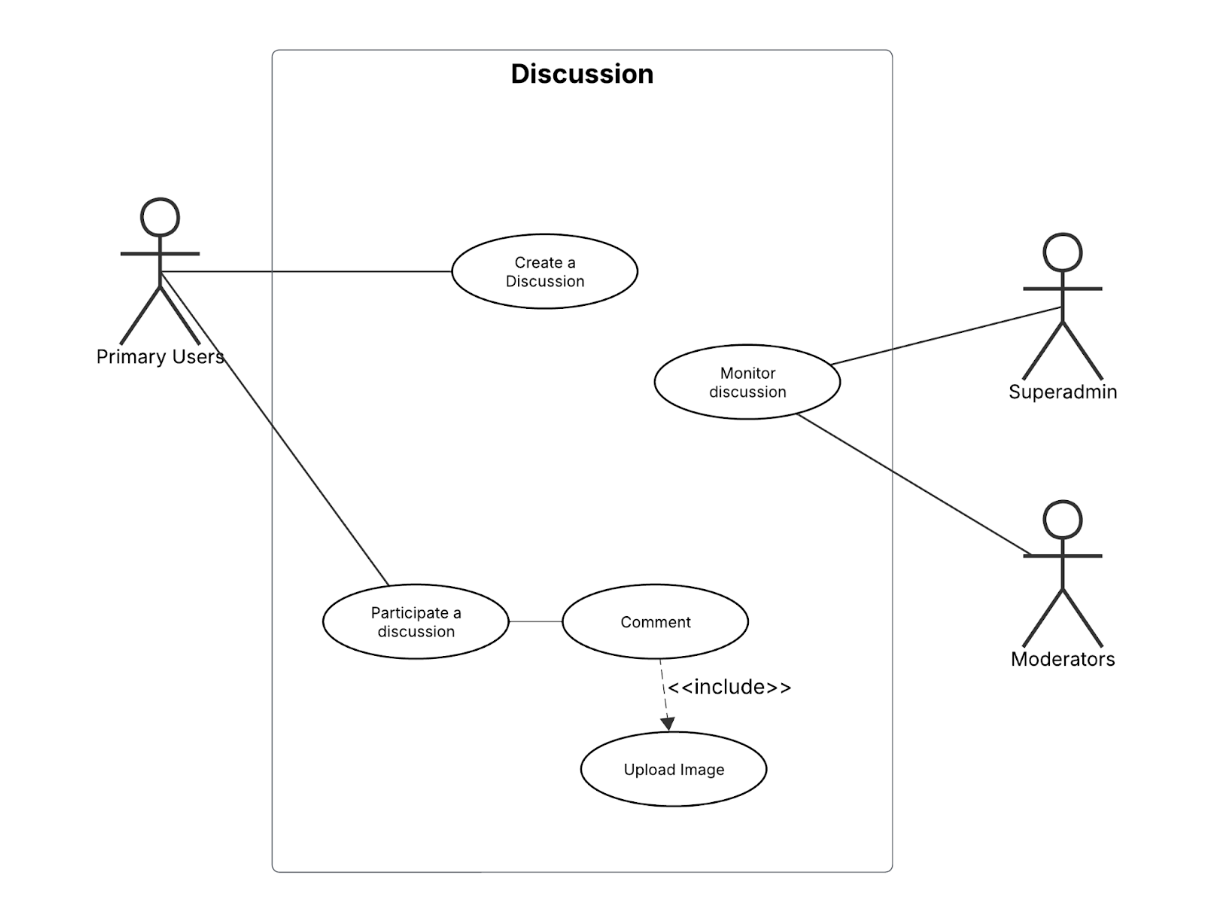
\includegraphics[width=1\textwidth]{Contents/Chapter 3/Usecase/Images/Discussion.png}
    \vspace{0.6cm}
    \caption{Discussion Use Case}
\end{figure}
The \textbf{Discussion submodule} helps make CodeRank a friendly and interactive community where users can learn from each other. With the Create Discussion feature, users can start new discussion threads about coding problems, programming ideas, or any tech-related topic. After a thread is created, others can join in by commenting on that thread. Comments can include rich content, such as images added, making explanations clearer and easier to follow.
To ensure that discussions remain constructive and aligned with community guidelines, the submodule integrates essential administrative controls. Both the Superadmin and Moderators utilize the Monitor Discussion function to oversee user activity, identify and address inappropriate content, and uphold the platform’s community standards. 

\clearpage

\begin{figure}[h!]
    \centering
    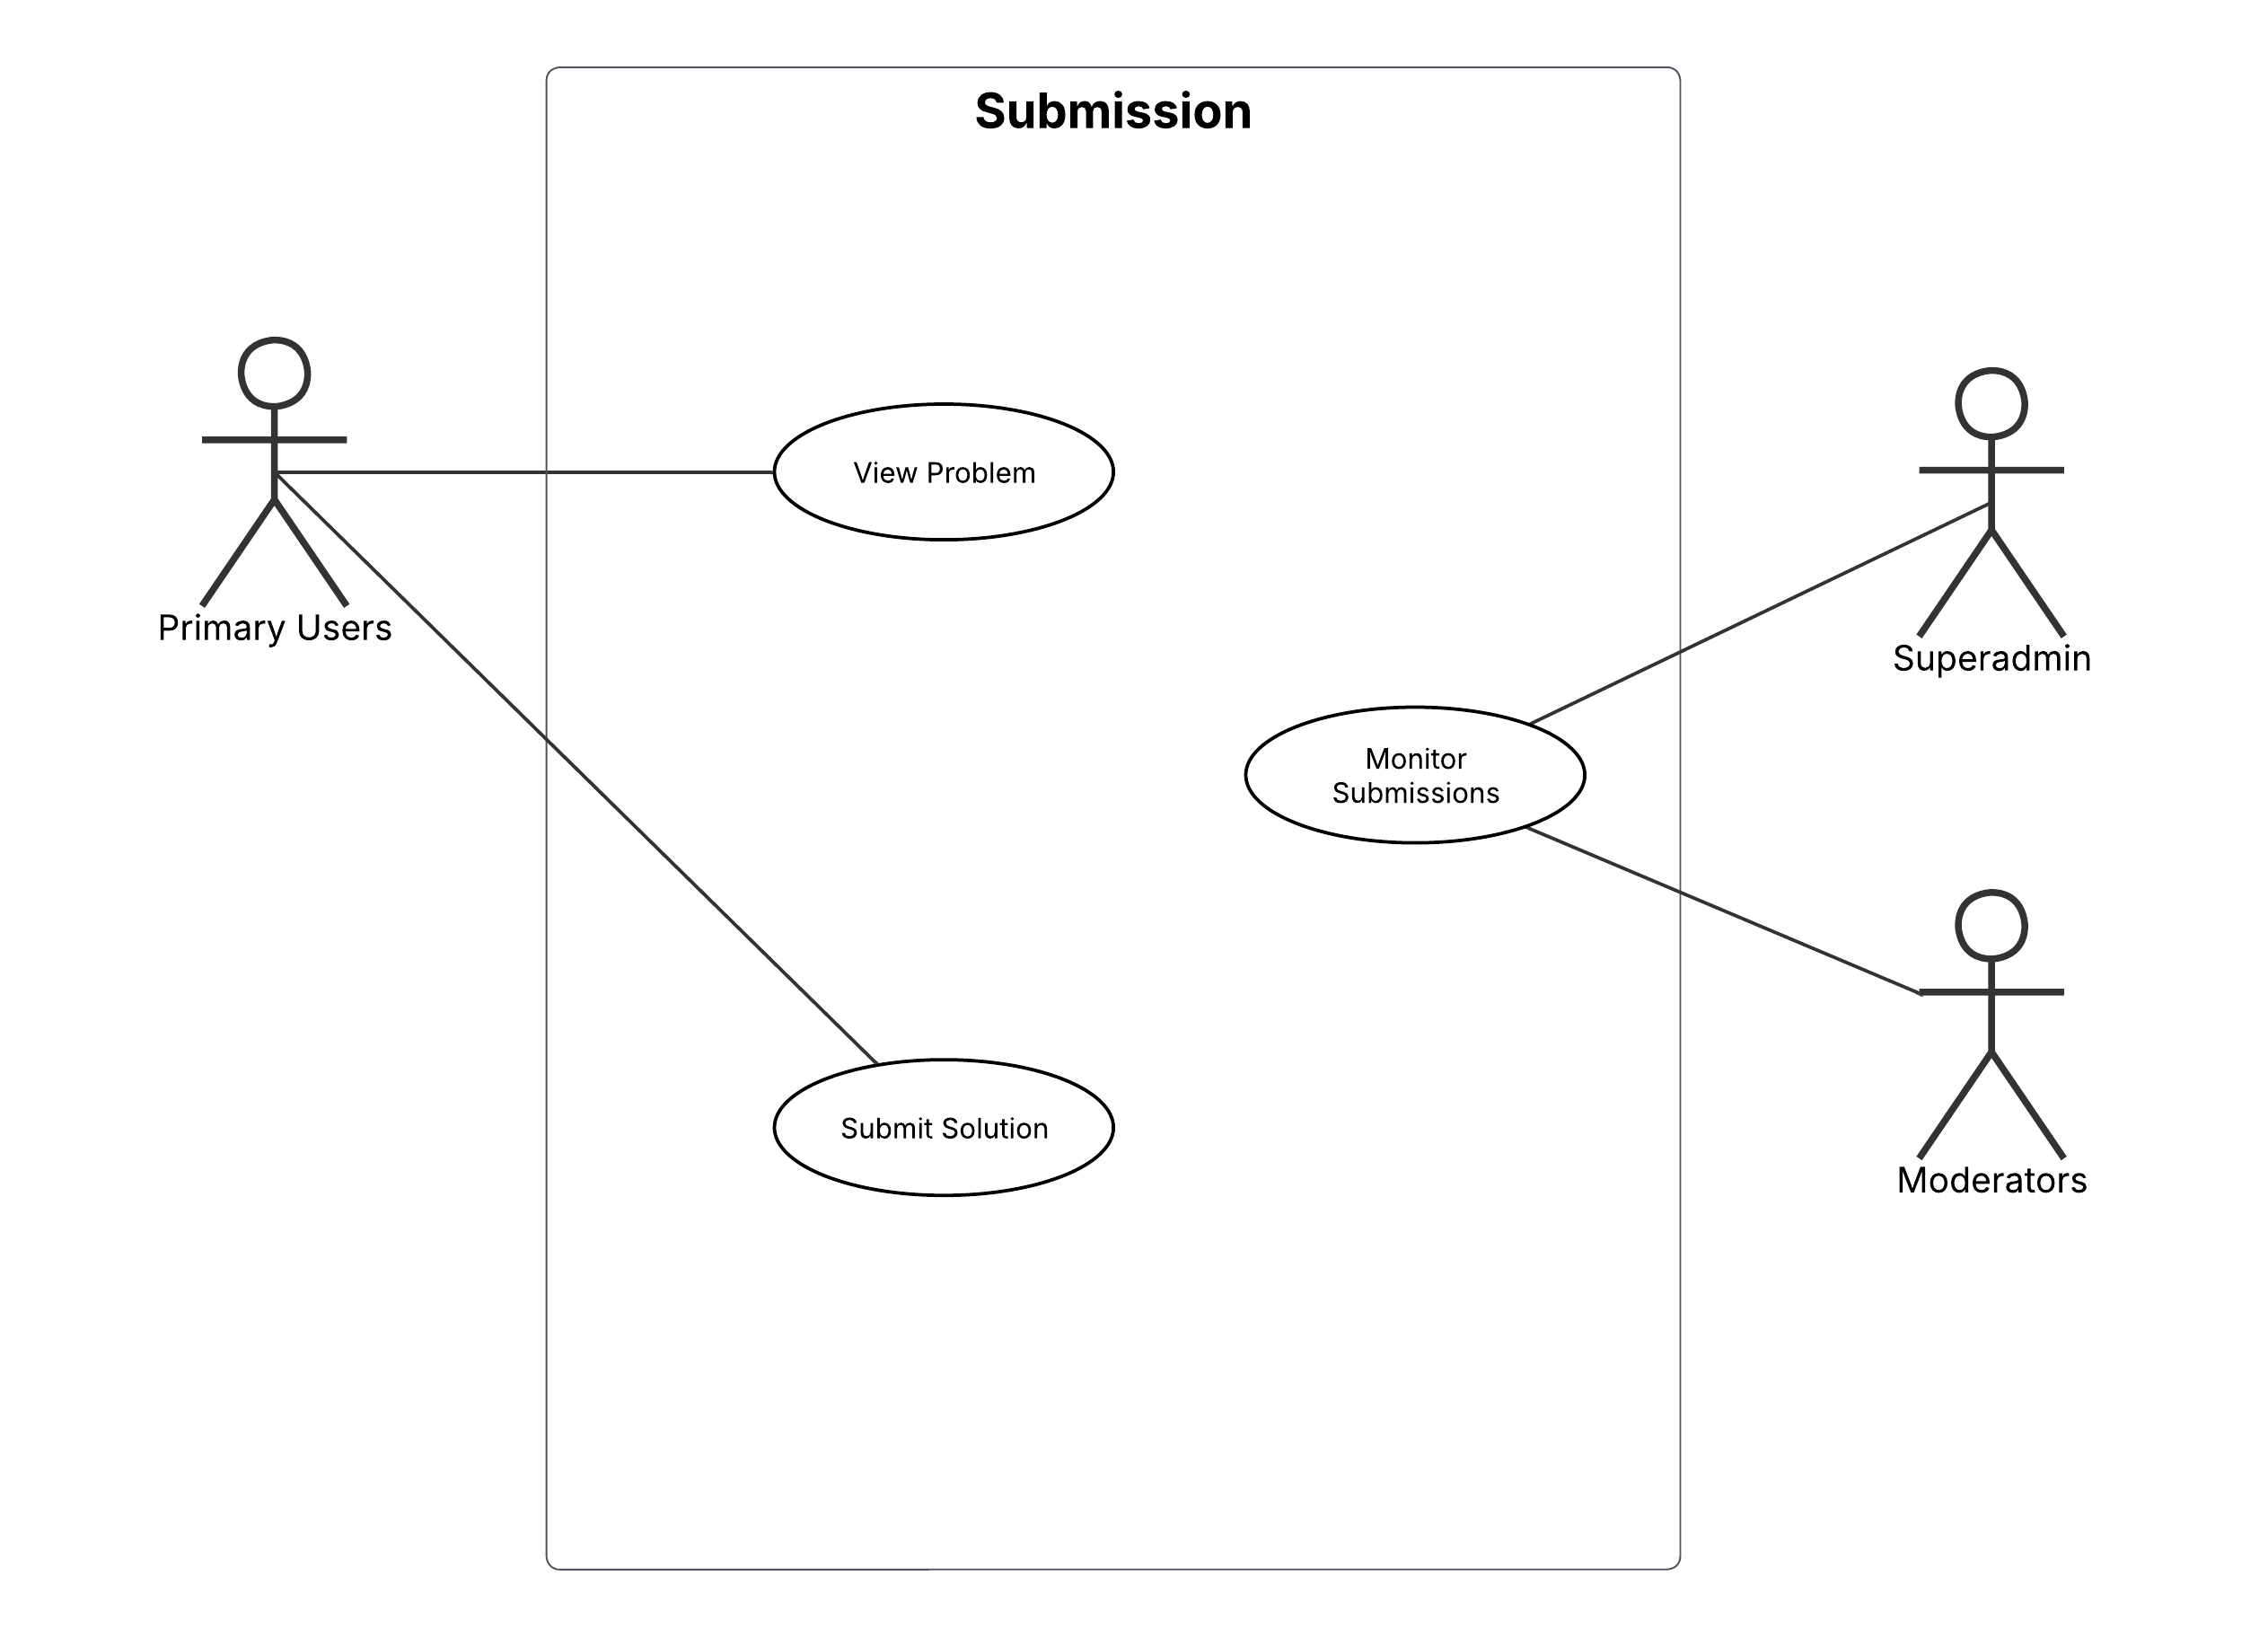
\includegraphics[width=1\textwidth]{Contents/Chapter 3/Usecase/Images/Submission.png}
    \vspace{0.6cm}
    \caption{Submission Use Case}
\end{figure}
The \textbf{Submission} submodule is the core execution engine and interaction point for all coding activities within the CodeRank system. Its primary function is to facilitate the practice and assessment workflow for the Primary User. Users begin by accessing the \textbf{View Problem} function, which presents the algorithmic challenge and requirements. The fundamental action in this module is the \textbf{Submit Solution} function, which securely receives the user's code, initiates the automatic grading process in a sandboxed environment, and returns the execution verdict. For oversight and quality assurance, both the Superadmin and Moderators are granted the ability to Monitor Submissions. This administrative function is vital for diagnosing issues with test cases, tracking potential cases of plagiarism, and ensuring the overall stability and fairness of the automated grading system.
\subsubsection{Use-case description tables}
% \begin{table}
% \caption{Use Case UC-1: Problems Management}
% \renewcommand{\arraystretch}{1.4}
% \begin{tabular}{|p{4cm}|p{11cm}|}
% \hline
% \textbf{ID and Name} & UC-1. Problems Management \\ \hline

% \textbf{Date Created} & 20th September, 2025 \\ \hline

% \textbf{Primary Actor} & Primary User, Superadmin, Moderator \\ \hline

% \textbf{Secondary Actor} & System (CodeRank Platform) \\ \hline

% \textbf{Description} &
% This use case describes how Moderators and Superadmins manage algorithmic problems on the platform. The process includes creating, editing, approving, and publishing problems. It also covers defining problem statements, input/output formats, constraints, sample test cases, and hidden test cases.
% \\ \hline

% \textbf{Trigger} &
% A Moderator or Superadmin decides to create, edit, approve, or publish a problem.
% \\ \hline

% \textbf{Preconditions} &
% \begin{itemize}
% \item The user is logged in as a Moderator or Superadmin.
% \item The problem management interface is accessible.
% \end{itemize}
% \\ \hline

% \textbf{Postconditions} &
% \begin{itemize}
% \item A new problem is created and saved as draft.
% \item A draft problem is updated or submitted for approval.
% \item A published problem may be updated after Superadmin approval.
% \item A problem is published once the approval rule is satisfied.
% \end{itemize}
% \\ \hline

% \textbf{Normal Flow} &
% \begin{enumerate}
% \item Moderator/Superadmin accesses the problem management interface.
% \item Moderator creates a new problem (saved as draft).
% \item Moderator edits draft problem (auto-saved).
% \item Moderator or Superadmin submits the problem for approval.
% \item Moderator approves problem → System checks publishing rule.
% \item If approvals >= 3 (Moderators) or 1 (Superadmin), system auto-publishes.
% \item Superadmin can directly approve and publish a problem.
% \end{enumerate}
% \\ \hline

% \textbf{Alternative Flow} &

% \textbf{AF–1:} Moderator edits a published problem → System saves changes as pending\_edit → Requires Superadmin approval. 

% \textbf{AF–2:} If approval threshold is not met, the problem stays pending until more approvals are collected.
% \\ \hline

% \textbf{Exceptions} &
% \textbf{E–1:} Superadmin rejects a pending edit → System notifies Moderator.
% \\ \hline
% \end{tabular}
% \end{table}


% \begin{table}
% \caption{Use Case UC-2: Contest Management}
% \renewcommand{\arraystretch}{1.3}
% \begin{tabular}{|p{4cm}|p{11cm}|}
% \hline
% \textbf{ID and Name} & UC-2. Contest Management \\ \hline

% \textbf{Date Created} & 20th September, 2025 \\ \hline

% \textbf{Primary Actor} & Primary User, Superadmin, Moderator \\ \hline

% \textbf{Secondary Actor} & System (CodeRank Platform) \\ \hline

% \textbf{Description} &
% This use case describes how users create and submit contests, allow administrators to review and approve them, and make contests available for participation once published.
% \\ \hline

% \textbf{Trigger} &
% A Primary User submits a new contest request.
% \\ \hline

% \textbf{Preconditions} &
% \begin{itemize}[nosep, leftmargin=*]
% \item The user is authenticated.
% \item Contest details (title, description, rules, problems) are provided.
% \item The contest submission form is valid.
% \end{itemize}
% \\ \hline

% \textbf{Postconditions} &
% \begin{itemize}[nosep, leftmargin=*]
% \item Contest status is updated (pending, approved, or published).
% \item Notifications are sent to users and admins.
% \item Users can participate in contests once published.
% \end{itemize}
% \\ \hline

% \textbf{Normal Flow} &
% \begin{enumerate}[nosep, leftmargin=*]
% \item Primary User submits a contest request.
% \item The System saves the contest as \textit{Pending Review}.
% \item Moderators review and approve the contest.
% \item If at least 3 moderator approvals are received, the contest qualifies for publishing.
% \item Alternatively, a Superadmin may approve and publish with a single approval.
% \item The System updates the contest status to \textbf{Published}.
% \item Notifications are sent to the contest creator and relevant moderators.
% \item Primary Users may now participate in the contest.
% \end{enumerate}
% \\ \hline

% \textbf{Alternative Flow} &
% \begin{itemize}[nosep, leftmargin=*]
% \item \textbf{AF-1: Insufficient Approvals}: If fewer than 3 moderator approvals are received, the contest remains in \textit{Pending Review}.
% \item \textbf{AF-2: Superadmin Override}: A Superadmin may publish directly, bypassing moderator approvals.
% \item \textbf{AF-3: Invalid Submission}: If contest data is incomplete or invalid, the submission is rejected with an error message.
% \end{itemize}
% \\ \hline

% \textbf{Exceptions} &
% \begin{itemize}[nosep, leftmargin=*]
% \item \textbf{E-1}: Database error when saving or updating the contest request.
% \item \textbf{E-2}: Approval action references a contest that does not exist.
% \item \textbf{E-3}: Notification delivery fails (system logs error, but contest status remains updated).
% \end{itemize}
% \\ \hline

% \end{tabular}
% \end{table}

% \begin{table}

% \renewcommand{\arraystretch}{1.3}
% \begin{tabular}{|p{4cm}|p{11cm}|}
% \caption{Use Case UC-3: Create a Discussion}
% \hline
% \textbf{ID and Name} & UC-3. Create a Discussion \\ \hline

% \textbf{Date Created} & 20th September, 2025 \\ \hline

% \textbf{Primary Actor} & Primary User \\ \hline

% \textbf{Secondary Actor} & System (CodeRank Platform) \\ \hline

% \textbf{Description} &
% This use case describes how a \textbf{Primary User} initiates a new discussion thread, typically linked to a specific problem ID or a general topic, setting the initial content and title.
% \\ \hline

% \textbf{Trigger} &
% The Primary User navigates to a problem page or the main forum and selects the \textit{"New Discussion"} option.
% \\ \hline

% \textbf{Preconditions} &
% \begin{itemize}[nosep, leftmargin=*]
% \item The user is authenticated.
% \item The discussion creation interface is accessible.
% \end{itemize}
% \\ \hline

% \textbf{Postconditions} &
% \begin{itemize}[nosep, leftmargin=*]
% \item A new discussion thread is created with the status \textit{"Active."}
% \item The discussion is visible to other Primary Users.
% \end{itemize}
% \\ \hline

% \textbf{Normal Flow} &
% \begin{enumerate}[nosep, leftmargin=*]
% \item Primary User accesses the problem/forum page and initiates creation.
% \item The user enters the discussion title and body content.
% \item The user submits the discussion.
% \item The system saves the new thread, assigns a unique ID, and displays it.
% \end{enumerate}
% \\ \hline

% \textbf{Alternative Flow} &
% \begin{itemize}[nosep, leftmargin=*]
% \item \textbf{AF-1: Content Validation Error}: If the title or body content is empty, the System displays an error message and requires the User to correct the input before submission.
% \end{itemize}
% \\ \hline

% \textbf{Exceptions} &
% \begin{itemize}[nosep, leftmargin=*]
% \item \textbf{E-1: Submission Failure}: If the database connection fails, the System displays a technical error and saves the content as a temporary draft (if possible).
% \end{itemize}
% \\ \hline

% \end{tabular}
% \end{table}

% \newpage

% \begin{table}[h!]
% \renewcommand{\arraystretch}{1.3}
% \begin{tabular}{|p{4cm}|p{11cm}|}
% \caption{Use Case UC-4: Submit a Solution}
% \hline
% \textbf{ID and Name} & UC-4. Submit a Solution \\ \hline

% \textbf{Date Created} & 20th September, 2025 \\ \hline

% \textbf{Primary Actor} & Primary User \\ \hline

% \textbf{Secondary Actor} & System (CodeRank Platform), Worker Service \\ \hline

% \textbf{Description} &
% This use case describes the primary mechanism for a \textbf{Primary User} to select a programming language, submit their solution code for a problem they are currently viewing, and receive an automated verdict on its correctness and efficiency.
% \\ \hline

% \textbf{Trigger} &
% The Primary User clicks the \textit{"Submit"} button on a coding problem interface after entering or selecting their solution code.
% \\ \hline

% \textbf{Preconditions} &
% \begin{itemize}[nosep, leftmargin=*]
% \item The user is authenticated.
% \item The user is currently viewing an active problem.
% \item The user has selected a supported programming language.
% \item The code is syntactically valid (pre-checked client-side).
% \end{itemize}
% \\ \hline

% \textbf{Postconditions} &
% \begin{itemize}[nosep, leftmargin=*]
% \item The submitted code is sent to the System.
% \item The Submission History is updated with the result (e.g., Accepted, Wrong Answer).
% \item The user's score and statistics are updated based on the verdict.
% \end{itemize}
% \\ \hline

% \textbf{Normal Flow} &
% \begin{enumerate}[nosep, leftmargin=*]
% \item Primary User is on the problem page and selects their preferred language.
% \item The user enters or pastes the solution code into the editor.
% \item The user clicks \textit{"Submit."}
% \item The system validates the submission (e.g., code length, language availability).
% \item The system sends the code and the problem's hidden test cases to the Worker Service.
% \item \textbf{Worker Service} securely executes the code and determines the verdict (e.g., Accepted, Time Limit Exceeded, Runtime Error).
% \item The system displays the final verdict and execution statistics to the Primary User.
% \end{enumerate}
% \\ \hline

% \textbf{Alternative Flow} &
% \begin{itemize}[nosep, leftmargin=*]
% \item \textbf{AF-1: Attempted Language Not Supported}:  
% If the user attempts to submit code in a language that is not currently enabled for the problem, the System displays an error and requires the user to change their language selection.
% \end{itemize}
% \\ \hline

% \textbf{Exceptions} &
% \begin{itemize}[nosep, leftmargin=*]
% \item \textbf{E-1: Submission Failure}:  
% If the sandbox environment or the external grading service fails during execution, the System logs the error and returns a \textit{"System Error"} verdict to the user, advising them to try again later.
% \end{itemize}
% \\ \hline

% \end{tabular}
% \end{table}


\newpage

\section{Architecture Diagram}
\subsection{Architectural Decision Rationale}
Architectural diagrams provide a structured view of how a software system is organized and how its components interact. In modern software development, two primary architectural styles are commonly considered: \textbf{monolithic architecture} and \textbf{microservice architecture}.

A \textbf{monolithic architecture} is a traditional model of a software program, which is built as a unified unit that is self-contained and independent from other applications. The word “monolith” is often attributed to something large and glacial, which isn’t far from the truth of a monolith architecture for software design. \cite{atlassian_microservices_vs_monolith}

A \textbf{microservices architecture}, also simply known as microservices, is an architectural method that relies on a series of independently deployable services. These services have their own business logic and database with a specific goal. Updating, testing, deployment, and scaling occur within each service. Microservices decouple major business, domain-specific concerns into separate, independent code bases. \cite{atlassian_microservices_vs_monolith}

As can be seen, the choice between these architectural approaches depends on the project’s specific requirements, team size, and long-term goals. Smaller systems or teams often benefit from the straightforwardness of monolithic architecture, while larger, more complex systems may require the flexibility and scalability of distributed services.

After evaluating our project goals and team size, we decided to implement a service-based modular monolith as the core architectural foundation for CodeRank. The key reasons for selecting this approach include:
\begin{itemize}
    \item \textbf{Team Size and Feasibility}
With only two members, adopting a full microservice architecture would introduce significant overhead in DevOps, deployment, and service management. In contrast, a modular monolith allows us to focus on implementing core features without the burden of distributed complexity.
    \item \textbf{Easier Development and Maintenance}
By separating the system into modules—such as the Discussion Module, Submission Module, Auth Module, and Contest Module—we can maintain clean boundaries within a single codebase. This structure enables faster development cycles and reduces merging conflicts.
    \item \textbf{Future Scalability}
While CodeRank currently operates as a monolithic application, its modules are designed following \textbf{Domain-Driven Design} (DDD) principles. These boundaries can later be extracted into microservices if the system needs to scale. This ensures long-term flexibility without requiring microservices prematurely.
\end{itemize}
\begin{figure}[h!]
    \centering
    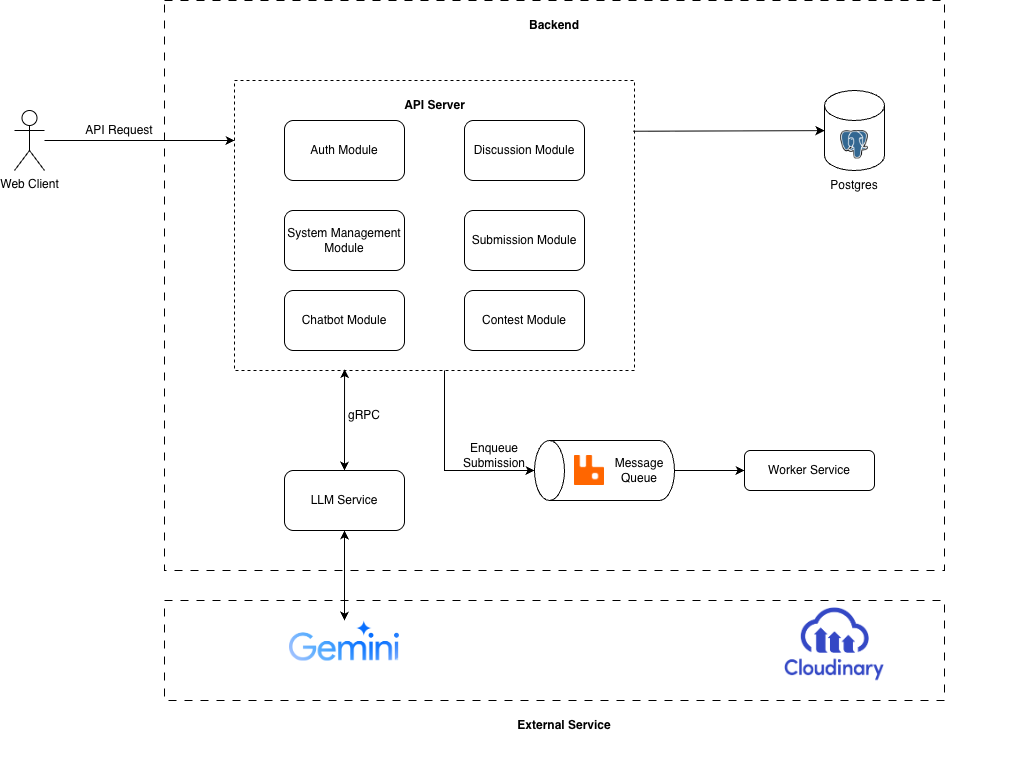
\includegraphics[width=1\textwidth]{Contents/Chapter 3/Architecture Diagram/CodeRank.drawio.png}
    \vspace{0.6cm}
    \caption{Architecture Diagram}
    \label{fig:leetcode-system}
\end{figure}
\clearpage

\subsection{System Components}

\begin{figure}[h!]
    \centering
    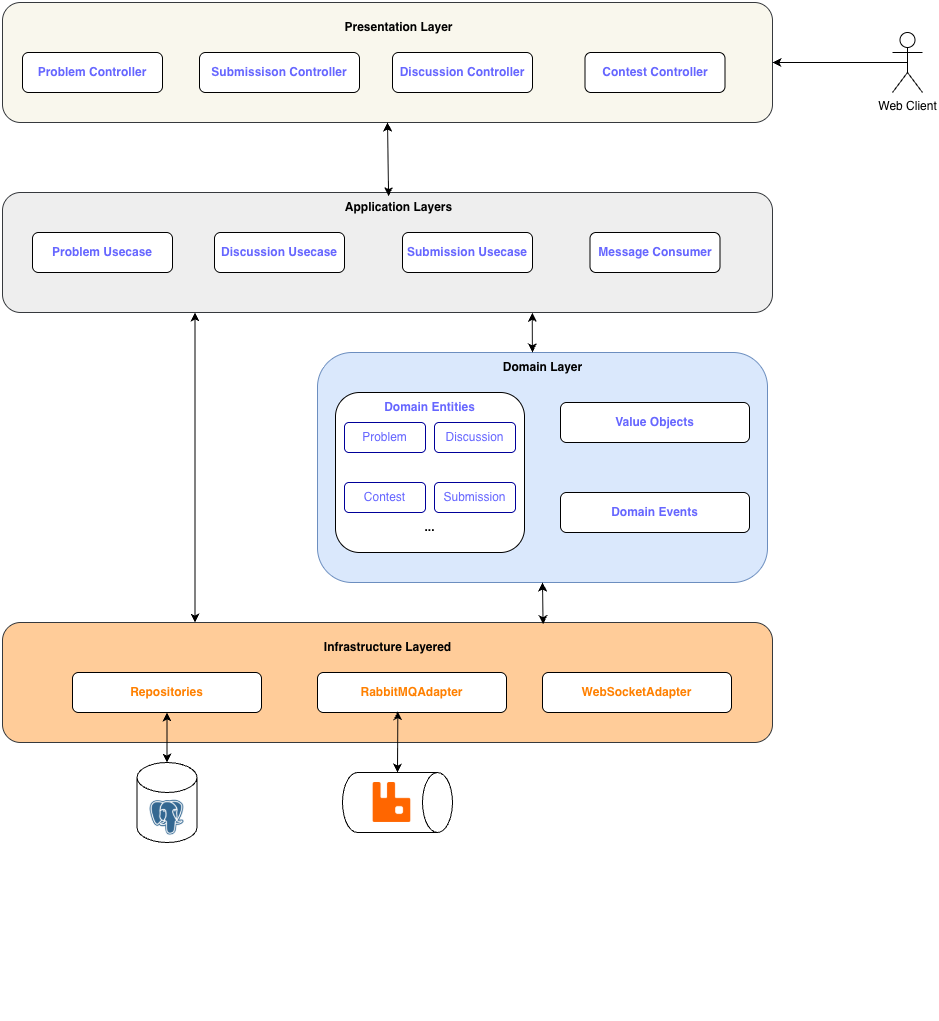
\includegraphics[width=1\textwidth]{Contents/Chapter 3/Architecture Diagram/LayeredArchitecture.drawio.png}
    \vspace{0.6cm}
    \caption{Layered Architecture}
    \label{fig:leetcode-system}
\end{figure}
The system architecture of CodeRank is organized into four primary layers, each responsible for a specific set of functions. This layered approach ensures clean separation of concerns, maintainability, and a clear mapping between business rules and system implementation.

\begin{enumerate}
  \item \textbf{Presentation Layer}
  
The \textbf{Presentation Layer} acts as the entry point for all external interactions with the system. It exposes various controllers such as the \textit{Problem Controller}, \textit{Submission Controller}, \textit{Discussion Controller}, and \textit{Contest Controller}, which handle incoming HTTP requests from the web client. These controllers validate user input, map requests to the appropriate application use cases, and return responses in a structured format. This layer focuses purely on communication and does not contain business logic, ensuring the interface remains thin and easily adaptable.
    \item  \textbf{Application Layer}
    
The \textbf{Application Layer} contains the system’s core orchestrators, known as Use Cases. Examples include the Problem Usecase, Discussion Usecase, Submission Usecase, and a dedicated Message Consumer for asynchronous tasks.

This layer coordinates operations between the Presentation Layer and the Domain Layer, ensuring that business rules are executed in the correct sequence. It does not implement business rules itself; instead, it acts as a mediator, invoking domain logic and triggering events. This design improves code clarity and supports future expansion.

    \item  \textbf{Domain Layer}
    
The \textbf{Domain Layer} represents the heart of the application, where all business logic and system rules are defined. It contains: 

\begin{itemize}
    \item Domain Entities such as Problem, Discussion, Contest, and Submission.
    \item Value Objects that encapsulate immutable attributes or concepts.
Domain Events used to capture and react to significant changes within the system.
    \item Domain Events used to capture and react to significant changes within the system.
\end{itemize}

    \item  \textbf{Infrastructure Layer}
    
The \textbf{Infrastructure Layer} provides the technical capabilities required to support the domain and application layers. It includes: 

\begin{itemize}
    \item \textbf{Repositories}, which manage communication with the PostgreSQL database.
    \item \textbf{RabbitMQ Adapters}, responsible for publishing and consuming messages for asynchronous processing.
Domain Events used to capture and react to significant changes within the system.
    \item \textbf{WebSocket Adapters}, enabling real-time communication such as live updates for submissions or discussion activities.
\end{itemize}

This layer abstracts external systems and framework-specific operations, ensuring that the upper layers remain decoupled from technical implementation details.

\end{enumerate}
\section{Code Runner}
\subsection{Overview}
\textbf{Code Runner} Component is a core component of Submission Worker Service, responsible for executing user-submitted programs against predefined test cases. It serves as a bridge between the user’s solution and the problem’s input–output data, ensuring fair and consistent evaluation. 
For each programming language supported by the platform (C++, Java, Python), a specific implementation of the \textbf{Code Runner} will be developed to handle language-specific compilation, execution, and output parsing. This ensures that user code is run correctly and consistently, regardless of the language chosen.
\subsection{Class Diagram}
\begin{figure}[h!]
    \centering
    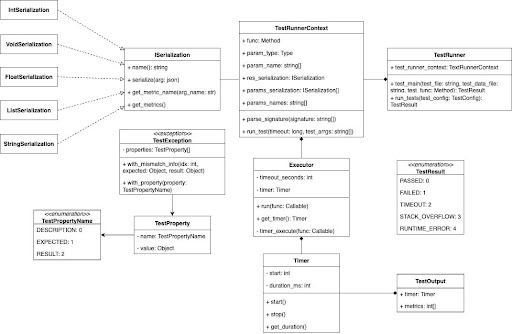
\includegraphics[width=1\textwidth]{Contents/Chapter 3/Code Runner/CodeRunner.jpg}
    \vspace{0.6cm}
    \caption{Class Diagram for Code Runner}
    \label{fig:leetcode-system}
\end{figure}

\begin{itemize}
    \item \textbf{ISerialization \& Implementations}: ISerialization defines a common interface for converting data between raw test inputs/outputs and program variables. Its implementations — IntSerialization, FloatSerialization, StringSerialization, ListSerialization, and VoidSerialization — handle serialization for different data types, ensuring test cases are interpreted correctly regardless of format.
    \item \textbf{TestRunnerContext}: TestRunnerContext stores the configuration and metadata needed to execute a user’s function, including parameter types, serializers, and the function reference itself. It prepares the environment for test execution and delegates the actual running to the Executor.
    \item \textbf{Executor}: Executor manages controlled execution of user-submitted functions. It enforces time limits, measures execution duration using Timer, and handles potential runtime issues like timeouts or errors during function calls.
    \item \textbf{Timer}: Timer measures how long each test case takes to execute. It provides simple start, stop, and duration tracking methods to record performance metrics for user solutions.
    \item \textbf{TestOutput}: TestOutput captures the results of a single test execution, storing both the runtime duration and any performance metrics. It is used to report how efficiently and accurately a user’s code performed.
    \item \textbf{TestException}: TestException represents errors or mismatches that occur during test execution. It stores details such as expected versus actual results and additional context through TestProperty objects.
    \item \textbf{TestProperty \& TestPropertyName}: TestProperty stores metadata about a test, such as a description or result comparison, identified by a TestPropertyName enum. These properties provide structured details for debugging failed test cases.
    \item \textbf{TestRunner}: TestRunner is the main controller responsible for running user code against predefined test cases. It coordinates between the TestRunnerContext, Executor, and ISerialization system to execute tests and produce final TestResult outcomes.
    \item \textbf{Solution}: Solution is the submission for the problem from the user.
\end{itemize}
\subsection{Testcase Format}
Each problem in the Online Judging System is accompanied by a test case file, named \textit{problem\_slug.csv}. This file defines a structured list of input–output test pairs used by the Test Runner of Worker Service to evaluate user submissions automatically.Moderators or superadmin upload this file when creating or updating a problem. The judging system parses the CSV, runs user code against each test case, and compares the output with the expected result.

To ensure accurate and consistent evaluation of user submissions, each input and output value in the \textit{problem\_slug.csv}file is associated with a data type. The type system defines how each field should be parsed, validated, and compared during the judging process.This mechanism helps the Test Framework interpret user program outputs correctly, whether they are numbers, strings, booleans, or lists. The following table describes the type.Here is the content for the "Problem Storages" section, including the table about type format:

\begin{table}[h!]
\centering
\renewcommand{\arraystretch}{1.3}
\begin{tabular}{|p{4cm}|p{10cm}|}
\hline
\textbf{Type Token} & \textbf{Description} \\ \hline

int & Integer numbers. \\ \hline

float & Floating-point numbers. \\ \hline

boolean & Boolean data. \\ \hline

string & Textual data. \\ \hline

void & Represents the absence of a value (e.g., for functions that return nothing). \\ \hline

list(type) & A collection of elements of a specified type (e.g., list(int)). \\ \hline

\end{tabular}
\caption{Data Types for Testcase Fields}
\end{table}
Each problem’s test case file will contain both type definitions for input, expected output and test data. The first line of the file specifies the data types for all inputs and outputs, helping the Test Runner correctly parse and validate values before running tests.

After executing all test cases for a user’s submission, the Test Runner generates a structured JSON result file summarizing the outcomes of each test. This file serves as the standardized output for the judging system and can be used by other services (such as the Result Service or API Gateway) to record, display, or analyze user performance. The JSON format ensures that results are machine-readable, language-independent, and easy to integrate into the overall online judging pipeline. The exported JSON file contains both metadata (e.g., problem name, language, execution status) and detailed per-test results (e.g., input, output, expected result, duration, and status).

\section{Ranking System}

The ranking system is a core component of the platform, designed to motivate users, reflect individual learning progress, and encourage healthy competition among participants. It provides a transparent and consistent mechanism for evaluating user performance based on problem-solving activities.

\subsection*{Overall Ranking Mechanism}

The platform maintains a global leaderboard that ranks all registered users based on their accumulated points obtained from solving programming problems. This leaderboard reflects the relative standing of users across the entire system and allows learners to compare their progress with others. However, to reduce server workload and avoid unnecessary real-time synchronization, the ranking data is not pushed to clients in real time.

Instead, the frontend retrieves ranking data through the backend API when users access or refresh the leaderboard page. The backend calculates or returns the latest available ranking data based on accepted submissions and accumulated user scores. This request-based approach keeps the implementation simple and efficient while still providing users with sufficiently updated ranking information during normal platform usage.

Although the leaderboard is not updated through real-time events, users can view their current score and ranking information whenever the relevant page or profile data is loaded from the backend. This design provides a practical balance between system performance, implementation complexity, and user experience.

\subsection*{Point Allocation per Problem}

Points are awarded based on the difficulty level of each problem. The platform categorizes problems into three difficulty levels, each associated with a predefined base score:
\begin{itemize}
    \item \textbf{Easy}: 100 points
    \item \textbf{Medium}: 150 points
    \item \textbf{Hard}: 200 points
\end{itemize}

This scoring scheme encourages users to challenge themselves with more complex problems while still recognizing achievements at all difficulty levels.

\subsection*{Penalty for Failed Submissions}

To promote code quality and thoughtful problem-solving, the system applies a penalty for unsuccessful submissions. A submission is considered failed if it does not pass all predefined test cases. For each failed submission attempt, a penalty of 10 points is deducted from the base score of the corresponding problem.

If the total penalty incurred from failed submissions exceeds the base score of the problem, the final score awarded for that problem is capped at 0 points. Negative scores are not applied. This mechanism discourages excessive trial-and-error submissions while still allowing users to continue practicing without additional penalties once the minimum score is reached.

\subsection*{First Successful Submission Policy}

Points are awarded only for the first successful submission of a problem, defined as the first submission that passes all test cases. Any subsequent successful submissions for the same problem are treated strictly as practice attempts and do not contribute additional points to the user’s total score.

This policy ensures fairness in the ranking system and prevents users from inflating their scores by repeatedly submitting solutions to the same problem. It also emphasizes learning progression through solving new problems rather than optimizing repeated submissions for ranking purposes.

\section{Database Design}

For data models design, we utilize Entity–Relationship Diagram (ERD) to capture the conceptual model of CodeRank System. It visualizes the core entities of the platform—such as users, problems, submissions, test cases, and judging results—and the relationships among them. The ERD serves a similar purpose to a UML class diagram, but at a higher level of abstraction. Therefore, including both diagrams would be redundant, and the ERD alone is sufficient for representing the system’s conceptual data structure.

The conceptual data model includes the following entities that will be grouped according to its business in our system. However, this diagram does not include all attributes of each entity for simplicity of illustration, but the essential ones are mentioned in the descriptions below.

\begin{figure}[H]
    \centering
    \rotatebox{90}{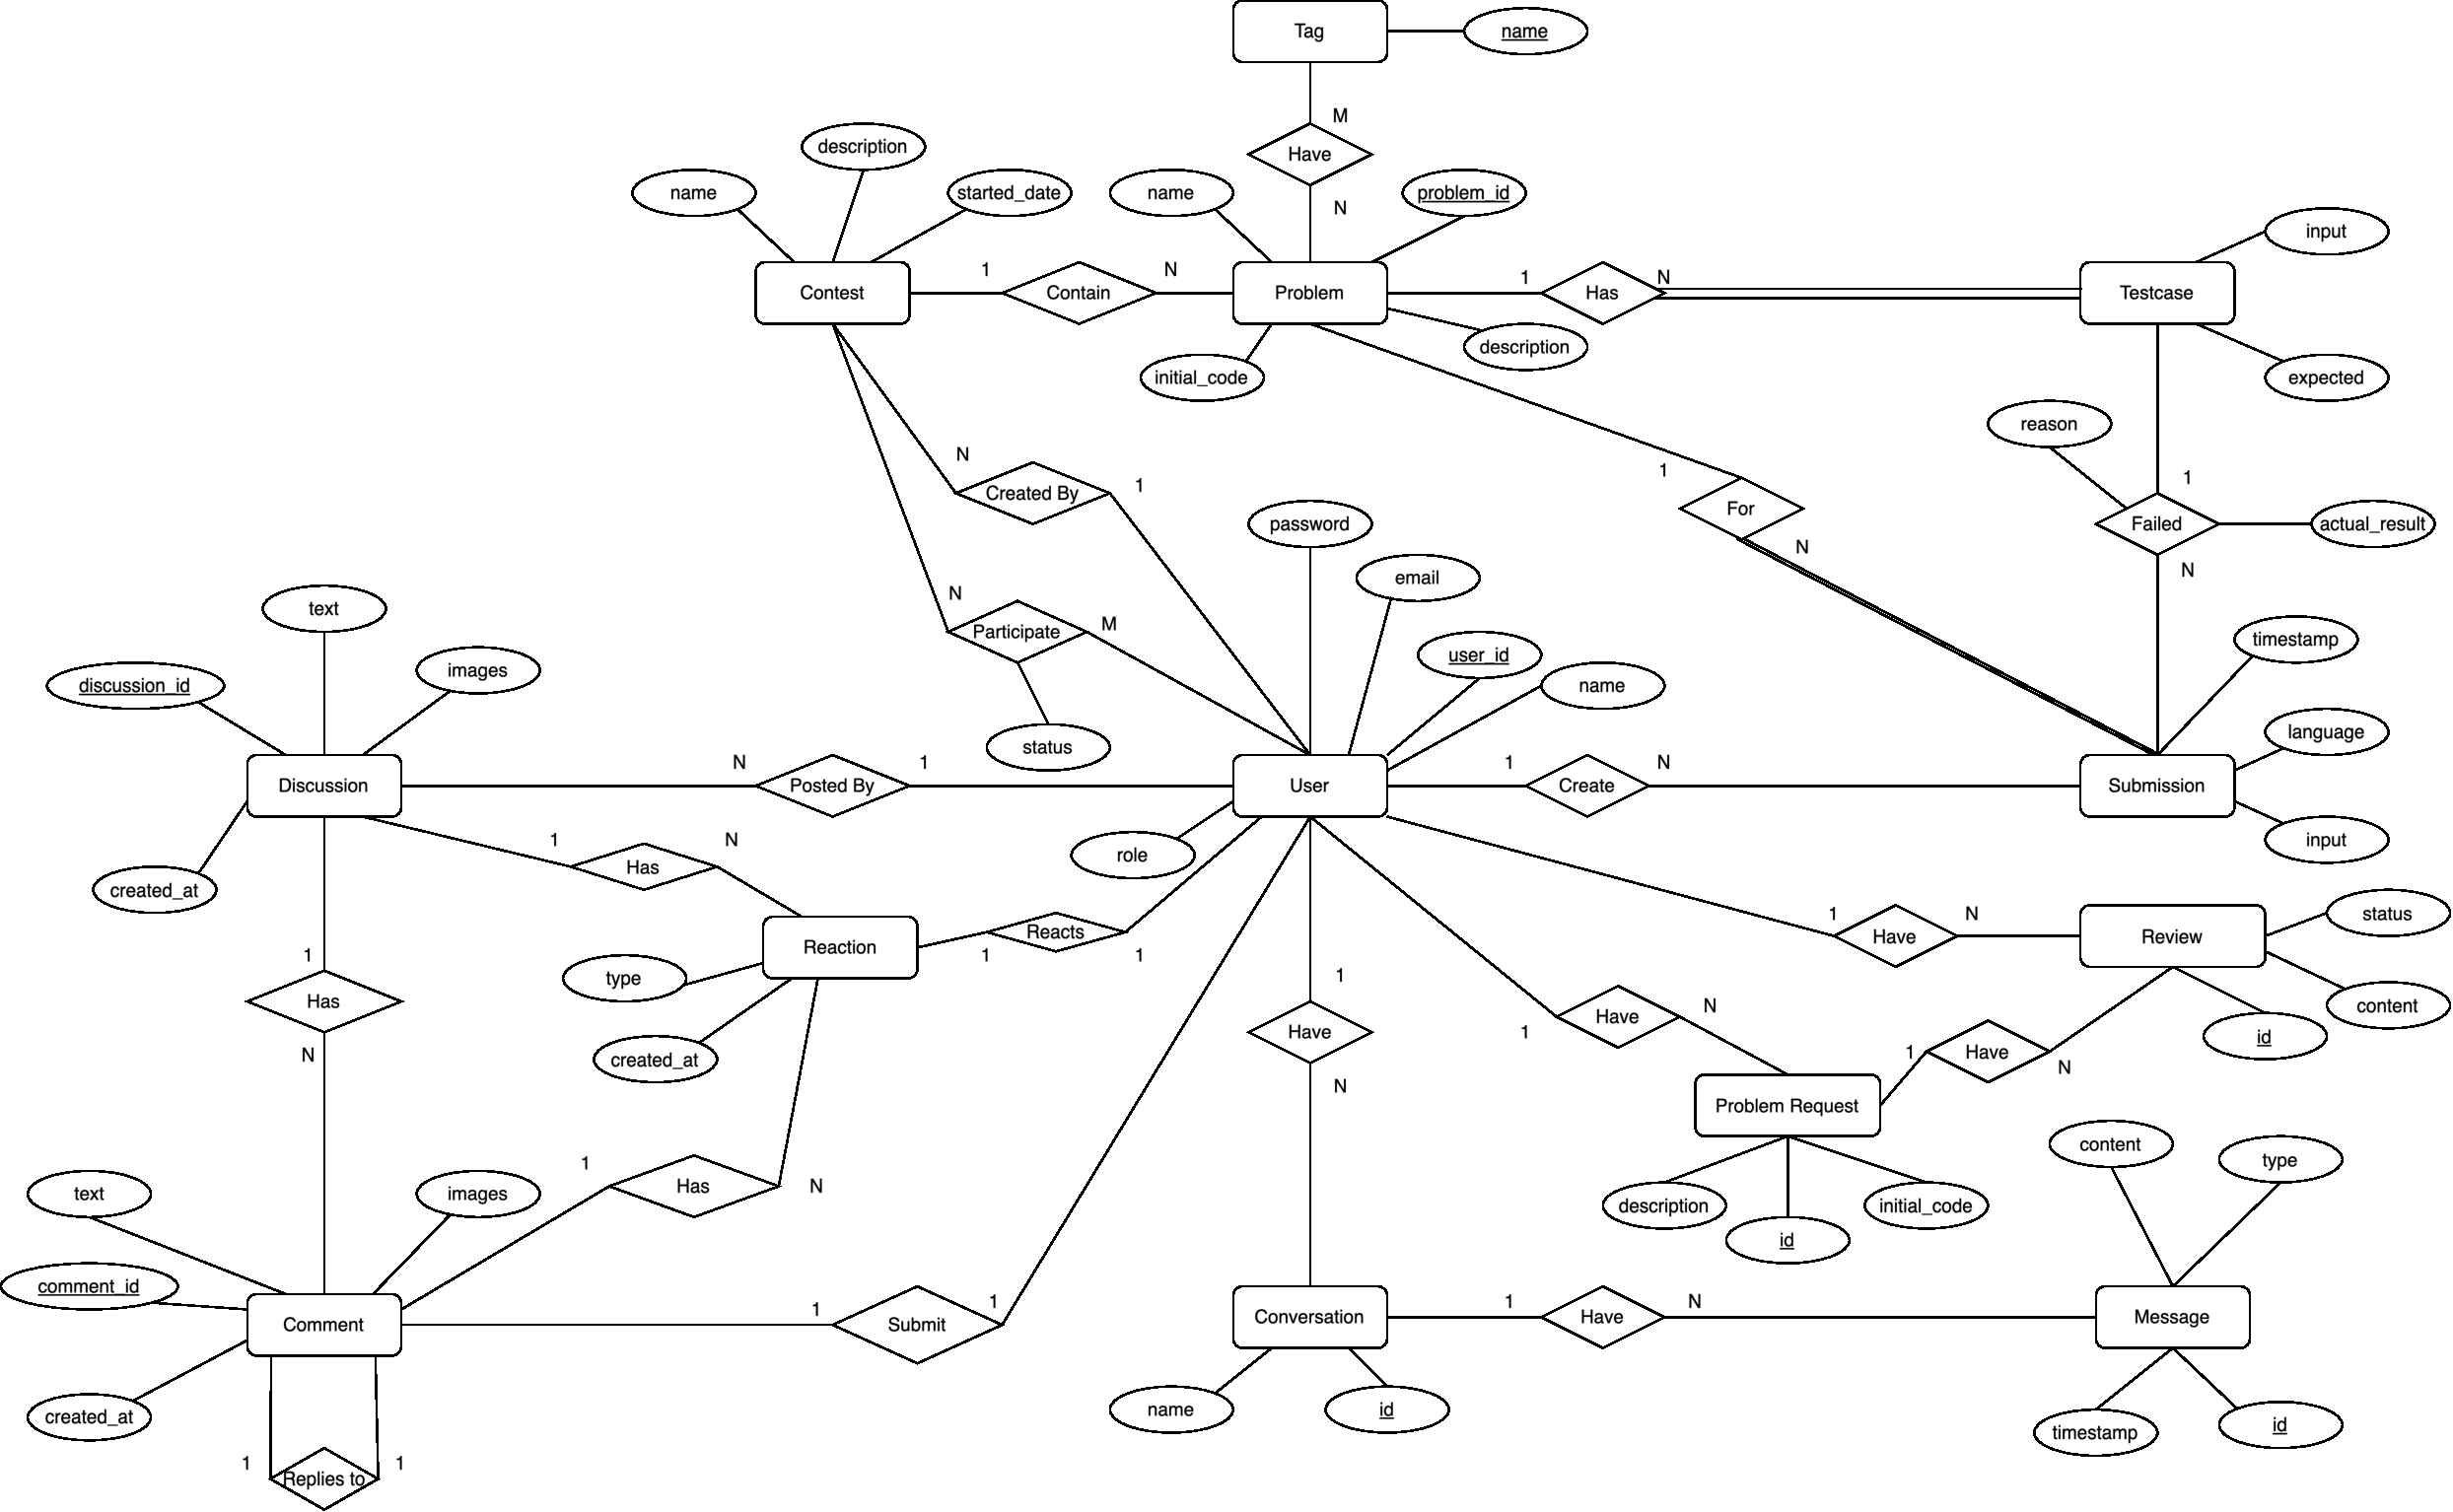
\includegraphics[width=\textheight]{Contents/Chapter 3/Database Design/erd.pdf}}
    \caption{Entity Relationship Diagram}
\end{figure}

\subsection*{User}
\begin{itemize}
    \item \textbf{User}: This abstract entity represents a user of the CodeRank system, storing essential information such as username, email, password hash. Each entity is identified by \textit{user\_id} For simplicity of illustration, we have omitter user roles and permissions in the ERD, all of this is represented by the attribute \textit{role} of the User entity. However, in the actual implementation, user roles and permissions will be managed through Role-Based Access Control (RBAC) to ensure secure and appropriate access to system functionalities.
\end{itemize}

\subsection*{Problems Solving}

\begin{itemize}
    \item \textbf{Problem}: Represents an algorithmic challenge that users can attempt to solve. Each problem includes a unique identifier \textit{problem\_id}, a title, a textual description, and optional starter code (\textit{initial\_code}) to guide users.
A problem may belong to multiple contests and can have multiple tags for classification.
    \item \textbf{Tag}: The \textit{Tag} entity helps organize problems into conceptual groups (for example, Dynamic Programming, String, etc). Each tag has a \textit{name} and may be associated with multiple problems through a many-to-many relationship.
    \item \textbf{Testcase}: Belongs to one problem and includes input data and the corresponding expected output. Testcases are used during code execution to validate user submissions.
    \item \textbf{Submission}: Represents a user's attempt to solve a problem. Each submission is linked to a specific user and problem, and includes the submitted code, programming language, timestamp, and status (e.g., pending, accepted, rejected).
\end{itemize}

\subsubsection*{Problems Management}

\begin{itemize}
    \item \textbf{Problem Request}: Represents a request made by a moderator or superadmin to add a new problem to the platform. Each request includes a title, description, and status (e.g., pending, approved, rejected). It is linked to the moderator or superadmin who made the request.
    \item \textbf{Review}: Represents the review process for a problem request. Each review is associated with a specific problem request and includes feedback, status (e.g., approved, rejected), and the timestamp of the review. It is linked to the moderator or superadmin who conducted the review.
\end{itemize}

\subsection*{Contest}
\begin{itemize}
    \item \textbf{Contest}: Represents a coding competition that users can participate in. Each contest includes a unique identifier \textit{contest\_id}, a title, description, start time, end time, and a list of problems included in the contest. A contest will contain many problems, anc can have many participants.
\end{itemize}

\subsection*{Interview Practice}

\begin{itemize}
    \item \textbf{Conversation}: Represents a coding interview session between a Primary User and chatbot system. Each conversation includes a unique identifier \textit{conversation\_id}, start time, end time. Each conversation is linked to the Primary User who initiated it.
    \item \textbf{Message}: Represents individual messages exchanged during a coding interview conversation. Each message includes a unique identifier \textit{message\_id}, timestamp, content, and type of the message. If the message comes from Primary User, the type will be \textit{user}, otherwise \textit{system}. Each message is linked to the conversation it belongs to.
\end{itemize}

\subsubsection*{Discussion}
\begin{itemize}
    \item \textbf{Discussion}: represents forum-like discussion threads associated with a topic. Users can post questions, explanations, optimization ideas, or clarifications. Each discussion entry may contain text and optional images, and it records creation timestamps.
    \item \textbf{Comment}: Users can comment on discussion threads, forming a threaded conversation system. Each comment includes text, optional images, and a timestamp.
    \item \textbf{Reaction}: Users can react to both discussions and comments using predefined reaction types (e.g., like, love, insightful). Each reaction records the type of reaction and the user who made it.
\end{itemize}

To summarize the relationships among these entities:
\begin{itemize}
    \item A \textbf{User} can \textbf{submit} multiple \textbf{Submission}.
    \item Each \textbf{Submission} is \textbf{linked} to one \textbf{User} and one \textbf{Problem}.
    \item A \textbf{Problem} can \textbf{have} multiple \textbf{Testcases} and can be \textbf{associated} with multiple \textbf{Tags}.
    \item A \textbf{Contest} can \textbf{have} multiple \textbf{Users} as participants.
    \item A \textbf{Contest} can \textbf{include} multiple \textbf{Problem}.
    \item A \textbf{Problem Request} is made by a \textbf{User} with moderator or superadmin role.
    \item A \textbf{Review} is \textbf{conducted} by a \textbf{User} with moderator or superadmin role for a specific \textbf{Problem Request}.
    \item A \textbf{Conversation} is \textbf{initiated} by a \textbf{User} with Primary role.
    \item A \textbf{Conversation} can have multiple \textbf{Messages}.
    \item A \textbf{Discussion} can have multiple \textbf{Comments} and \textbf{Reactions}, and each \textbf{Comment} can also have multiple \textbf{Reactions}.
    \item A \textbf{Tag} can be associated with multiple \textbf{Problems}.
\end{itemize}


\section{Chatbot Design}
\subsection{Overview}
A chatbot, short for "chat robot", is an artificial intelligence (AI) software designed to simulate conversations with human users, especially over the internet. They interact with humans in their natural languages, typically through messaging applications, mobile apps or through a website. Chatbots can be programmed to respond the same way each time, to respond differently to messages containing specific keywords, or to use machine learning to adapt their responses to fit the situation. \cite{chatbot_definition}

In the context of CodeRank System, the chatbot is an AI-powered interactive interview coach designed to assist learners practicing technical coding interviews, particularly algorithm problems. The system leverages Google Gemini as the underlying large language model (LLM) and LangChain as the orchestration framework that structures prompts, manages conversational flow, and implements contextual memory.

The goal of the chatbot is to simulate real interview scenarios through step-by-step dialogue, enabling learners to experience guided practice, receive hints, refine answers, and develop a deeper understanding of algorithmic problem-solving techniques. To achieve human-like interaction, the chatbot must:
\begin{enumerate}
    \item Understand user inputs
    \item Maintain awareness of previous exchanges
    \item Adapt its questioning based on user responses
    \item Provide constructive and relevant feedback
    \item Prevent context loss during long interview sessions
\end{enumerate}

\subsection{Use case analysis}
To ensure consistent behavior and maintain the structured flow of a technical interview, the chatbot uses a System Prompt, also known as a behavioral instruction prompt. This prompt defines the chatbot's role as an AI interview coach and outlines the rules that govern how it interacts with the user. The following system prompt defines the chatbot's role and behavior during the structured mock interview process:
\begin{tcolorbox}[
    colback=white,      % White background
    colframe=black,     % Black border
    boxrule=0.8pt,      % Border thickness
    breakable,          % Allow page breaks
    sharp corners,      % Square corners
    listing only,       % Use listings engine
    listing options={
        basicstyle=\ttfamily\small,
        breaklines=true,      % Wrap long lines
        columns=fullflexible  % Prevent overflow
    }
]
\begin{verbatim}
You are an AI interview coach for coding interviews.
Your job is to conduct a structured mock interview.

Rules:
1. The FIRST message you receive from the user is the topic they want
to practice (e.g., arrays, dynamic programming, graphs).

2. After the user chooses a topic, ask ONE coding problem at a time.

3. After giving a question:
   - Wait for the user’s solution attempt.
   - Do NOT evaluate until the user submits a solution.
   - If the user is not ready, ask them to type their solution 
   when ready.

4. Provide hints ONLY when:
   - The user explicitly asks for a hint, OR
   - The user gives 3 incorrect attempts.

5. After the user solves (or gives up), provide:
   - A concise explanation
   - Optimal solution
   - Time complexity
   - Space complexity

6. Stay in interview mode.
\end{verbatim}
\end{tcolorbox}

To support a smooth and structured technical interview experience, the chatbot must be able to recognize different categories of user intentions. For the interview practice module of the CodeRank System, we classify user intents into three primary types: topic selection, problem-solving intent, and hint-seeking behavior. Each intent triggers a specific dialogue pattern that aligns with the structured mock interview workflow.

\textbf{Topic Selection Intent:} When users explicitly mention an interview topic, 
such as arrays, graphs, or dynamic programming, the system interprets this as an 
intention to begin or switch an interview topic. The chatbot should confirm the 
topic and proceed to present an appropriate coding problem. The possible questions are “Let’s practice arrays.”, “I want to try a dynamic 
programming problem.”, “Graphs.”, ...

\textit{For example when the user wants to find a topic to practice:}

\begin{quote}
\textbf{User:} Find me an array problem.\\
\textbf{Chatbot:} Sure! We'll practice arrays. Here is your first problem: 
\textit{Given an integer array…} Please let me know when you're ready to 
provide your solution.
\end{quote}

If the user provides additional details, the chatbot refines the difficulty:

\begin{quote}
\textbf{User:} Give me an easy array problem.\\
\textbf{Chatbot:} Great! Here is an easy-level array problem for you…
\end{quote}

\textbf{Problem-Solving Intent:} Once a coding problem has been presented, the user may 
respond with a complete solution, partial reasoning, or follow-up questions. This indicates 
the intention to solve the problem. The chatbot should acknowledge the attempt, avoid 
evaluating prematurely, and respond only after the user explicitly submits their solution. Possible user messages include “Here is my solution…”, “Does this approach work?”, 
or “I think we can use two pointers.”

\textit{For example when the user wants to submit a solution:}

\begin{quote}
\textbf{User:} Here is my solution: \texttt{...code...}\\
\textbf{Chatbot:} Thanks! Let me review your solution.
\end{quote}

If the user is still thinking:

\begin{quote}
\textbf{User:} I'm not ready yet.\\
\textbf{Chatbot:} No problem—take your time. Let me know when you're ready to submit 
your solution.
\end{quote}

If the attempt is incorrect, the chatbot guides without revealing too much:

\begin{quote}
\textbf{Chatbot:} This is not fully correct. Try again—pay attention to the edge case 
where the array may contain duplicates.
\end{quote}

\textbf{Hint-Seeking Intent:} When the user explicitly asks for help or expresses that they 
are stuck, the system recognizes this as an intention to request a hint. According to the 
interview rules, hints should only be provided when requested or after three unsuccessful 
attempts. Possible user messages include “Give me a hint.”, “I’m stuck.”, or “Can you guide me?”

\textit{For example when the user requests assistance:}

\begin{quote}
\textbf{User:} I’m stuck. Give me a hint.\\
\textbf{Chatbot:} Sure! Here’s a hint: Try using a hash map to store the frequencies of 
elements before making your decision.
\end{quote}

If the user is unclear about what type of hint they need:

\begin{quote}
\textbf{User:} I need help.\\
\textbf{Chatbot:} Of course. Would you like a conceptual hint, or guidance on improving 
your current approach?
\end{quote}

\section{Chatbot Design}

This chapter presents the detailed architecture, design decisions, and implementation of the chatbot subsystem in the CodeRank system. The chatbot is designed as an AI-powered coding interview assistant capable of simulating real-world technical interview scenarios.

Unlike traditional rule-based chatbots, the proposed system leverages a large language model combined with a workflow orchestration layer to enable adaptive reasoning, contextual memory, and dynamic response generation. This allows the system to behave as an intelligent interviewer that can guide users through structured problem-solving processes.

\subsection{N8N Integration Architecture}

The chatbot subsystem is implemented on top of \textbf{n8n}, which acts as a central orchestration layer connecting the frontend interface, backend services, and the Gemini large language model.

Instead of establishing a direct communication channel between the frontend and the LLM provider, all chatbot requests are routed through n8n workflows. This architectural decision introduces a middleware layer responsible for handling request processing, prompt management, memory retrieval, and response generation logic.

By decoupling AI logic from application layers, the system achieves better separation of concerns and improves maintainability in large-scale development.

\textbf{System Benefits:}
\begin{itemize}
    \item \textbf{Separation of Concerns:} AI logic is isolated from frontend and backend business logic, reducing system coupling.
    
    \item \textbf{Centralized Workflow Management:} All chatbot-related logic is managed in a single workflow system, making it easier to modify prompts, behaviors, and processing rules.
    
    \item \textbf{Improved Maintainability:} Changes in AI behavior do not require modifications in frontend or backend codebases.
    
    \item \textbf{Observability:} n8n provides execution logs at each node level, enabling easier debugging and monitoring of AI interactions.
\end{itemize}

\textbf{Chatbot Communication Flow:}
\begin{enumerate}
    \item The user interacts with the chatbot through the CodeRank frontend interface.
    
    \item The frontend sends the user message along with metadata to a backend API endpoint.
    
    \item The backend validates the request and triggers an n8n workflow via a webhook.
    
    \item The n8n workflow processes the request through a series of structured nodes.
    
    \item The workflow communicates with the Gemini model to generate context-aware responses.
    
    \item The final response is returned through the backend API and rendered in the frontend interface.
\end{enumerate}

This layered architecture enables independent evolution of system components, allowing AI logic, backend services, and frontend interfaces to be updated without affecting each other significantly.

\subsection{AI Agent Workflow Design in n8n}

The chatbot workflow is designed as an AI agent pipeline that simulates structured human-like reasoning during technical interview sessions. The workflow is composed of multiple modular stages, where each stage is responsible for a specific transformation or processing step.

This design follows a pipeline-based architecture, ensuring that input processing, context management, reasoning, and output generation are clearly separated.

\textbf{Workflow Stages:}
\begin{enumerate}
    \item User input reception
    \item Context and memory retrieval
    \item Prompt construction
    \item LLM processing
    \item Response post-processing
    \item Response delivery
\end{enumerate}

Each stage plays a critical role in ensuring that the chatbot maintains coherence, contextual awareness, and domain-specific behavior during long interview sessions.

\subsubsection{Webhook Trigger}

The workflow begins with a \textbf{Webhook Trigger Node}, which serves as the entry point for all incoming chatbot requests.

This node receives HTTP requests from the backend containing structured data such as:
\begin{itemize}
    \item User message content
    \item Conversation identifier for session tracking
    \item Interview context or selected topic
    \item User-related metadata (e.g., difficulty level, session state)
\end{itemize}

The webhook ensures that every interaction is properly initialized within the workflow execution context, enabling traceability and session continuity.

\subsubsection{Context and Memory Management}

One of the key challenges in conversational AI systems is maintaining context across multiple turns of interaction. To address this, the system implements a memory management mechanism within the workflow.

Before generating a response, the system retrieves relevant historical data including:
\begin{itemize}
    \item Previously asked interview questions
    \item User-submitted solutions or attempts
    \item Feedback and hints provided by the system
    \item Current interview progression state
\end{itemize}

This memory mechanism allows the chatbot to maintain consistency across long sessions and avoid treating each message as an isolated input. As a result, the AI behaves more like a continuous interviewer rather than a stateless response generator.

\subsubsection{Prompt Construction}

After retrieving contextual information, the system constructs a structured prompt that will be sent to the large language model.

The prompt construction process combines multiple sources of information:
\begin{itemize}
    \item System-level instructions defining chatbot behavior
    \item Current user input message
    \item Conversation history retrieved from memory
    \item Interview state and difficulty configuration
\end{itemize}

This step is crucial because prompt quality directly impacts the performance and consistency of the LLM output. By explicitly structuring the prompt, the system ensures that Gemini follows the expected interview logic and generates responses aligned with the CodeRank learning objectives.

\subsubsection{LLM Processing with Gemini}

The constructed prompt is passed to the \textbf{Google Gemini Chat Model node} within n8n. This node is responsible for interacting with the Gemini API and generating the final response based on the provided context.

The Gemini model performs multiple reasoning tasks simultaneously, including:
\begin{itemize}
    \item Understanding user intent in a programming context
    \item Generating coding interview questions dynamically
    \item Providing step-by-step hints for problem-solving
    \item Evaluating user approaches and suggesting optimizations
\end{itemize}

Depending on the state of the conversation, the model can act as an interviewer, tutor, or evaluator, allowing flexible adaptation to different learning scenarios.

\subsubsection{Response Post-processing}

After receiving the output from the LLM, the system performs a post-processing stage to ensure that the response is suitable for frontend rendering.

This includes:
\begin{itemize}
    \item Formatting output into Markdown-compatible structure
    \item Removing unnecessary tokens or artifacts
    \item Validating response completeness and structure
    \item Logging interaction data for debugging and analytics
\end{itemize}

This step ensures that the final response is clean, consistent, and user-friendly when displayed in the chatbot interface.

\subsubsection{Frontend Delivery}

The final processed response is returned through the backend API to the frontend application. The frontend then renders the response in real time within the chat interface.

This completes the full request-response cycle, enabling an interactive and low-latency conversational experience for users during coding interview sessions.

\subsection{System Design Benefits}

The proposed chatbot architecture provides several important system-level advantages:

\begin{itemize}
    \item \textbf{Modular Architecture:} Each stage of the workflow is independently defined, allowing easy modification and extension without affecting the entire system.
    
    \item \textbf{Scalability:} The system can be extended to support additional AI features such as retrieval-augmented generation (RAG), multi-agent collaboration, or external knowledge integration.
    
    \item \textbf{Maintainability:} Centralized workflow logic reduces code duplication and simplifies long-term maintenance.
    
    \item \textbf{Flexibility:} New AI behaviors can be introduced by modifying workflow nodes without changing core application code.
    
    \item \textbf{Observability:} Built-in execution tracking in n8n provides transparency in each step of the AI pipeline, facilitating debugging and system optimization.
\end{itemize}

Overall, the architecture enables the development of a robust, extensible, and production-ready AI chatbot system that is suitable for technical interview training and educational purposes.

\clearpage

\chapter {System Implementation}
\noindent
\rule{\textwidth}{0.4pt}

\begin{center}
\begin{minipage}{0.8\textwidth}
\textit{Chapter 4 presents the system implementation, describing how the proposed design is realized in practice. It includes the API design, which defines standardized communication between system components using the OpenAPI Specification; the backend structure, which explains the modular organization of the server-side codebase; the chatbot implementation, which integrates backend services with the n8n AI workflow; and the mockup design, which illustrates the user interface and interaction flow. Together, these components demonstrate the complete and cohesive implementation of the system.}
\end{minipage}

\end{center}

\section{API Design}

To ensure consistency with industry standards and facilitate efficient collaboration, the system adopts the OpenAPI Specification (version 3) to define and document all developed APIs. Based on this specification, the Swagger interface is integrated into the backend service, providing an interactive environment where developers and clients can explore, test, and understand the available endpoints.

As illustrated, the Swagger UI serves as a centralized and up-to-date documentation platform, allowing developers and integrators to quickly access API details such as request parameters, response formats, and authentication requirements. This approach significantly improves development efficiency, reduces integration complexity, and ensures better communication between frontend and backend components.

\begin{figure}[h!]
    \centering
    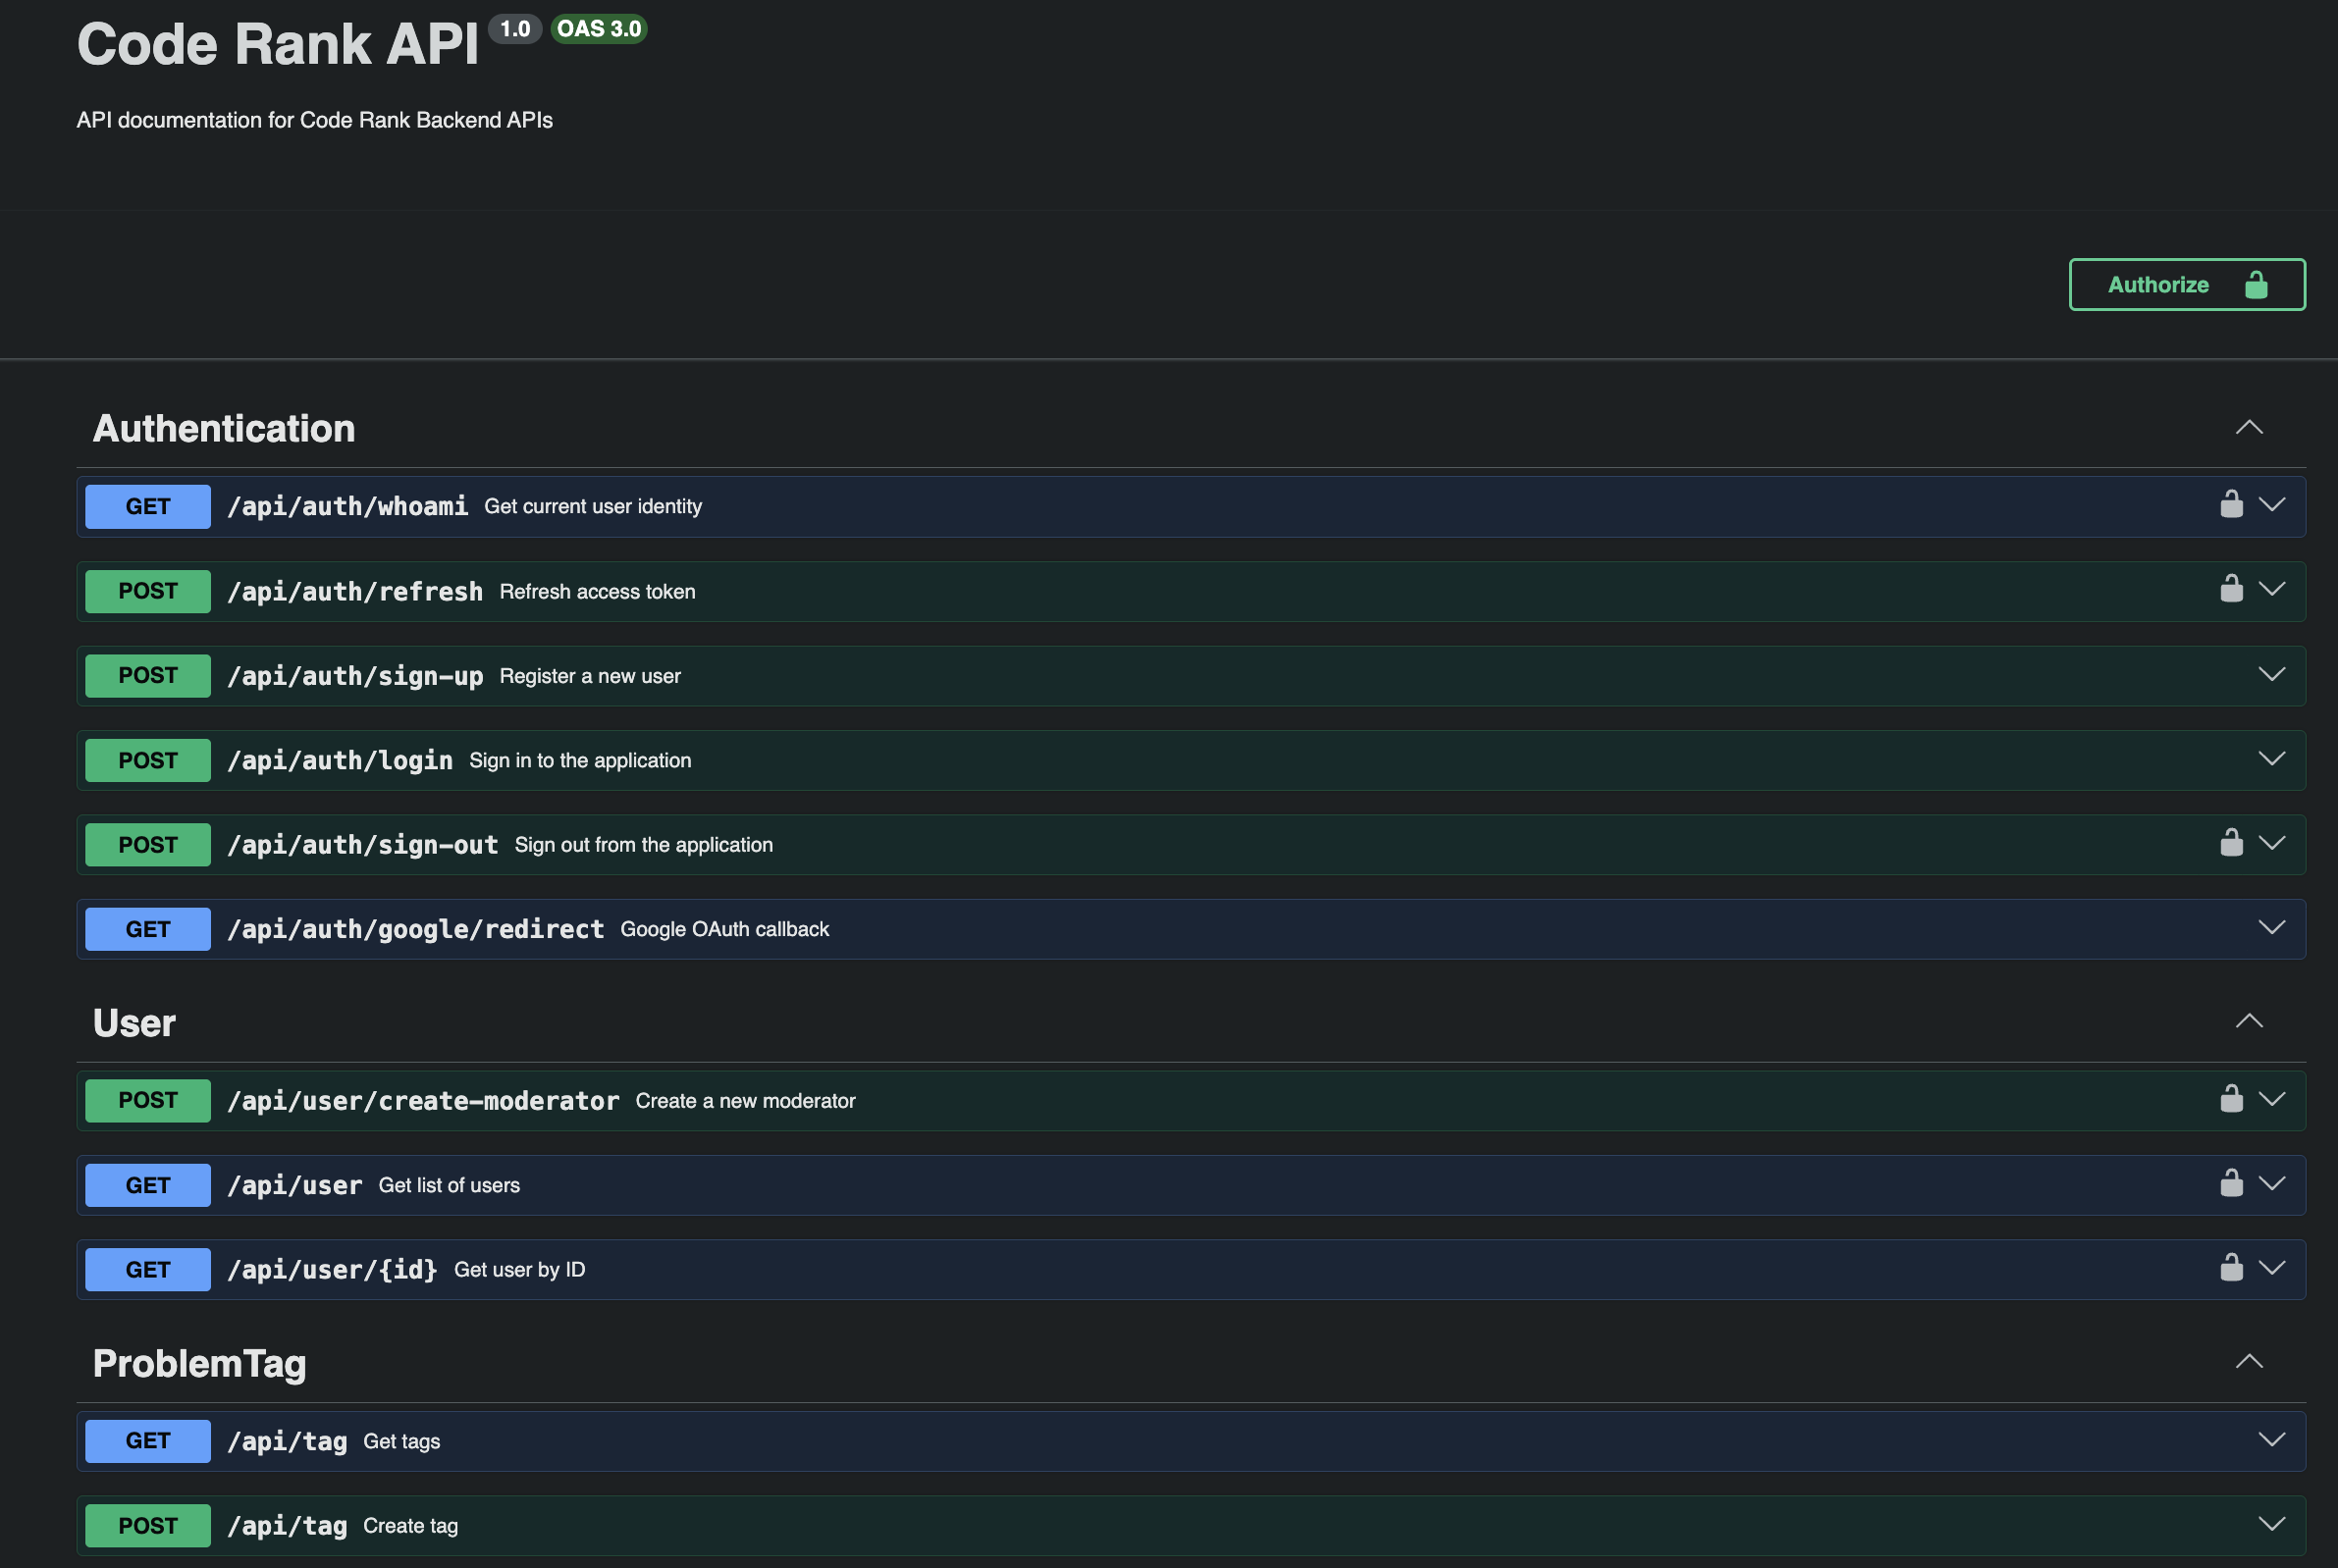
\includegraphics[width=1\textwidth]{Contents/Chapter 4/API Design/SwaggerApi.png}
    \vspace{0.6cm}
    \caption{API Swagger}
\end{figure}

\break
\section{Backend Structure}

The backend is implemented in TypeScript using a modular, Domain-Driven Design (DDD) approach built on a NestJS-style module pattern. The codebase is organized to reflect clear bounded contexts, a shared kernel for cross-cutting concerns, and an internals layer for platform services and infrastructure. This separation improves maintainability, testability, and team ownership.

\subsection{Architecture Overview}

At the highest level, the project is split into three logical layers:

\begin{enumerate}
	\item \textbf{Domain Layer}
	\item \textbf{Shared / Kernel Layer}
	\item \textbf{Internals / Infrastructure Layer}
\end{enumerate}

\subsection{Domain Layer}

This layer contains the core business logic and domain models, organized by bounded contexts under \texttt{domains}.

Each domain (for example: \texttt{auth}, \texttt{problem}, \texttt{submission}, \texttt{thread}, \texttt{user}) typically includes:

\begin{itemize}
	\item Controllers
	\item Services (use-case / application services)
	\item DTOs (Data Transfer Objects)
	\item Mappers
	\item Interfaces
	\item Domain-specific utilities
\end{itemize}

\subsection{Shared / Kernel Layer}

The shared layer contains reusable, domain-agnostic building blocks under \texttt{shared} and acts as a shared kernel to ensure reuse while keeping domain logic decoupled from framework specifics.

It includes:

\begin{itemize}
	\item Aggregate root patterns (e.g. \texttt{shared/aggregate})
	\item Base entities (e.g. \texttt{shared/entity})
	\item Common exceptions and constants
	\item Generic mappers
\end{itemize}

\subsection{Internals / Infrastructure Layer}

This layer contains platform-level concerns and infrastructure adapters under \texttt{internals}.

Common responsibilities:

\begin{itemize}
	\item Configuration (for example, \texttt{configuration.ts})
	\item Database setup and entity wiring (\texttt{database})
	\item Core framework services (\texttt{core})
	\item Infrastructure integrations (message brokers, external systems)
\end{itemize}

\subsection{Bounded Contexts and Module Responsibilities}

Each domain module represents a bounded context with clear ownership of its business logic.

\subsubsection{Auth Module}
\begin{itemize}
    \item Register and authenticate users (sign-up / sign-in).
    \item Issue, refresh, and revoke tokens / sessions.
    \item Validate and authorize requests based on roles/permissions.
    \item Enforce authentication-related business rules (e.g., account linking, password policies).
\end{itemize}


\subsubsection{Chatbot Module}
\begin{itemize}
    \item Intended to handle CRUD for AI conversation lifecycle (messages, sessions, histories).
    \item Acts as an adapter between HTTP controllers and an AI agent service (conversation orchestration).
    \item Stores or references conversation state and metadata for retrieval and continuation.
    \item Handle async processing and retries for AI responses.
    \item Integrates with infrastructure for calling external AI APIs and with message brokers for async tasks.
\end{itemize}

\subsubsection{Problem Module}
\begin{itemize}
    \item Create, update, publish, and archive problems.
    \item Manage problem metadata (tags, testcases, difficulty, reviews).
    \item Provide read models for public consumption and management views for editors.
    \item Validate problem inputs and maintain consistency of testcases and constraints.
\end{itemize}

\subsubsection{Submission Module}
\begin{itemize}
    \item Accept and record solution submissions from users.
    \item Queue and coordinate evaluation / judging workflows.
    \item Store and expose submission results, logs, and execution metadata.
    \item Handle retries, timeouts, and result aggregation for judging.
\end{itemize}

\subsubsection{Thread Module}
\begin{itemize}
    \item Create and manage discussions and comment threads.
    \item Support reactions/likes and moderation actions (edit/delete/report).
    \item Query and paginate discussions, comments, and thread metadata.
    \item Enforce posting rules and notification triggers for thread activity.
\end{itemize}

\subsubsection{User Module}
\begin{itemize}
    \item Manage user profiles, settings, and preferences.
    \item Handle user registration, authentication, and authorization.
    \item Provide user listing, search, and administrative controls.
    \item Enforce privacy, role-based access, and moderation policies.
\end{itemize}

\break
\section{Chatbot Implementation}

This section describes the detailed implementation of the chatbot subsystem in the CodeRank system. The implementation focuses on enabling real-time, streaming-based conversational interaction between the user and the AI assistant.

The chatbot is implemented using a multi-layer architecture consisting of the frontend client, backend API server, n8n workflow engine, and Gemini large language model. A key feature of the system is the use of Server-Sent Events (SSE) to support streaming responses, providing a real-time chat experience similar to modern AI assistants.

\subsection{End-to-End Chatbot Request Flow}

When a user interacts with the chatbot, the system processes the request through the following sequence:

\begin{enumerate}
    \item The user submits a message from the frontend chatbot interface.
    
    \item The frontend immediately sends the message to the backend API server using an HTTP request.
    
    \item The backend receives the request and initiates a processing pipeline by calling an internal chatbot service.
    
    \item The backend triggers an n8n workflow via a webhook, passing the user input and conversation metadata.
    
    \item n8n processes the request and communicates with the Gemini model to generate a response.
    
    \item The response is streamed back from n8n to the backend.
    
    \item The backend forwards the streamed response to the frontend using Server-Sent Events (SSE).
    
    \item The frontend renders the response incrementally in real time as tokens are received.
\end{enumerate}

This architecture ensures low-latency interaction and improves user experience by allowing the response to appear progressively instead of waiting for the full output.

\subsection{Backend Processing and Streaming Architecture}

The backend plays a critical role in managing request orchestration and enabling real-time response streaming.

After receiving the request from the frontend, the backend does not wait for the full response from the AI pipeline. Instead, it establishes a Server-Sent Events (SSE) connection with the client and acts as a streaming proxy between n8n and the frontend.

The backend performs the following tasks:

\begin{itemize}
    \item Validates incoming chatbot requests
    \item Forwards the request to the n8n webhook endpoint
    \item Receives streamed response chunks from n8n
    \item Forwards each chunk to the frontend via SSE channel
\end{itemize}

This streaming mechanism allows the system to handle long AI-generated responses efficiently while maintaining responsiveness.

\subsection{n8n Workflow Execution and Streaming Response}

Within the n8n workflow, the chatbot request is processed through multiple stages including context retrieval, prompt construction, and LLM inference.

Unlike traditional synchronous APIs, the integration is designed to support incremental response generation. As the Gemini model produces output, n8n streams partial results back to the backend instead of waiting for the full completion.

This streaming behavior is essential for enabling real-time chat experiences and reducing perceived latency.

The workflow acts as an intermediate layer that:
\begin{itemize}
    \item Receives user input from the backend via webhook
    \item Processes conversational context and memory
    \item Sends structured prompts to the Gemini model
    \item Streams generated tokens or response chunks back to the backend
\end{itemize}

\subsection{Frontend Streaming with Server-Sent Events (SSE)}

On the frontend side, the chatbot interface establishes a persistent SSE connection with the backend.

When a user sends a message, the frontend immediately displays a loading state and begins listening for streamed response events.

As the backend receives chunks of data from n8n, it forwards them to the frontend incrementally. The frontend then appends each received chunk to the chat interface in real time.

This results in a typewriter-like effect where the response appears progressively, significantly improving user experience compared to traditional request-response models.

The SSE-based approach provides the following benefits:
\begin{itemize}
    \item Low latency response rendering
    \item Improved perceived system performance
    \item Smooth real-time interaction experience
    \item Reduced waiting time for long AI outputs
\end{itemize}

\section{Mockup Design}

Mockup Design is a low-fidelity visual representation of a user interface that outlines the basic structure and layout of a digital product without focusing on visual design elements such as colors, typography, or imagery. Mockup Designs serve as a blueprint for developers and designers, defining the placement of content, navigation elements, and interactive components. This section will cover the Mockup Designs for two main user flows: \textit{Primary User flow} and \textit{Moderator/Admin flow} .

\subsection{Primary User flow}
\subsubsection*{Login}

Before accessing the application, users are required to login using their credentials. The Login Page will include 2 options based on role: Moderator/Admin login and User login.
\begin{figure}[H]
    \centering
    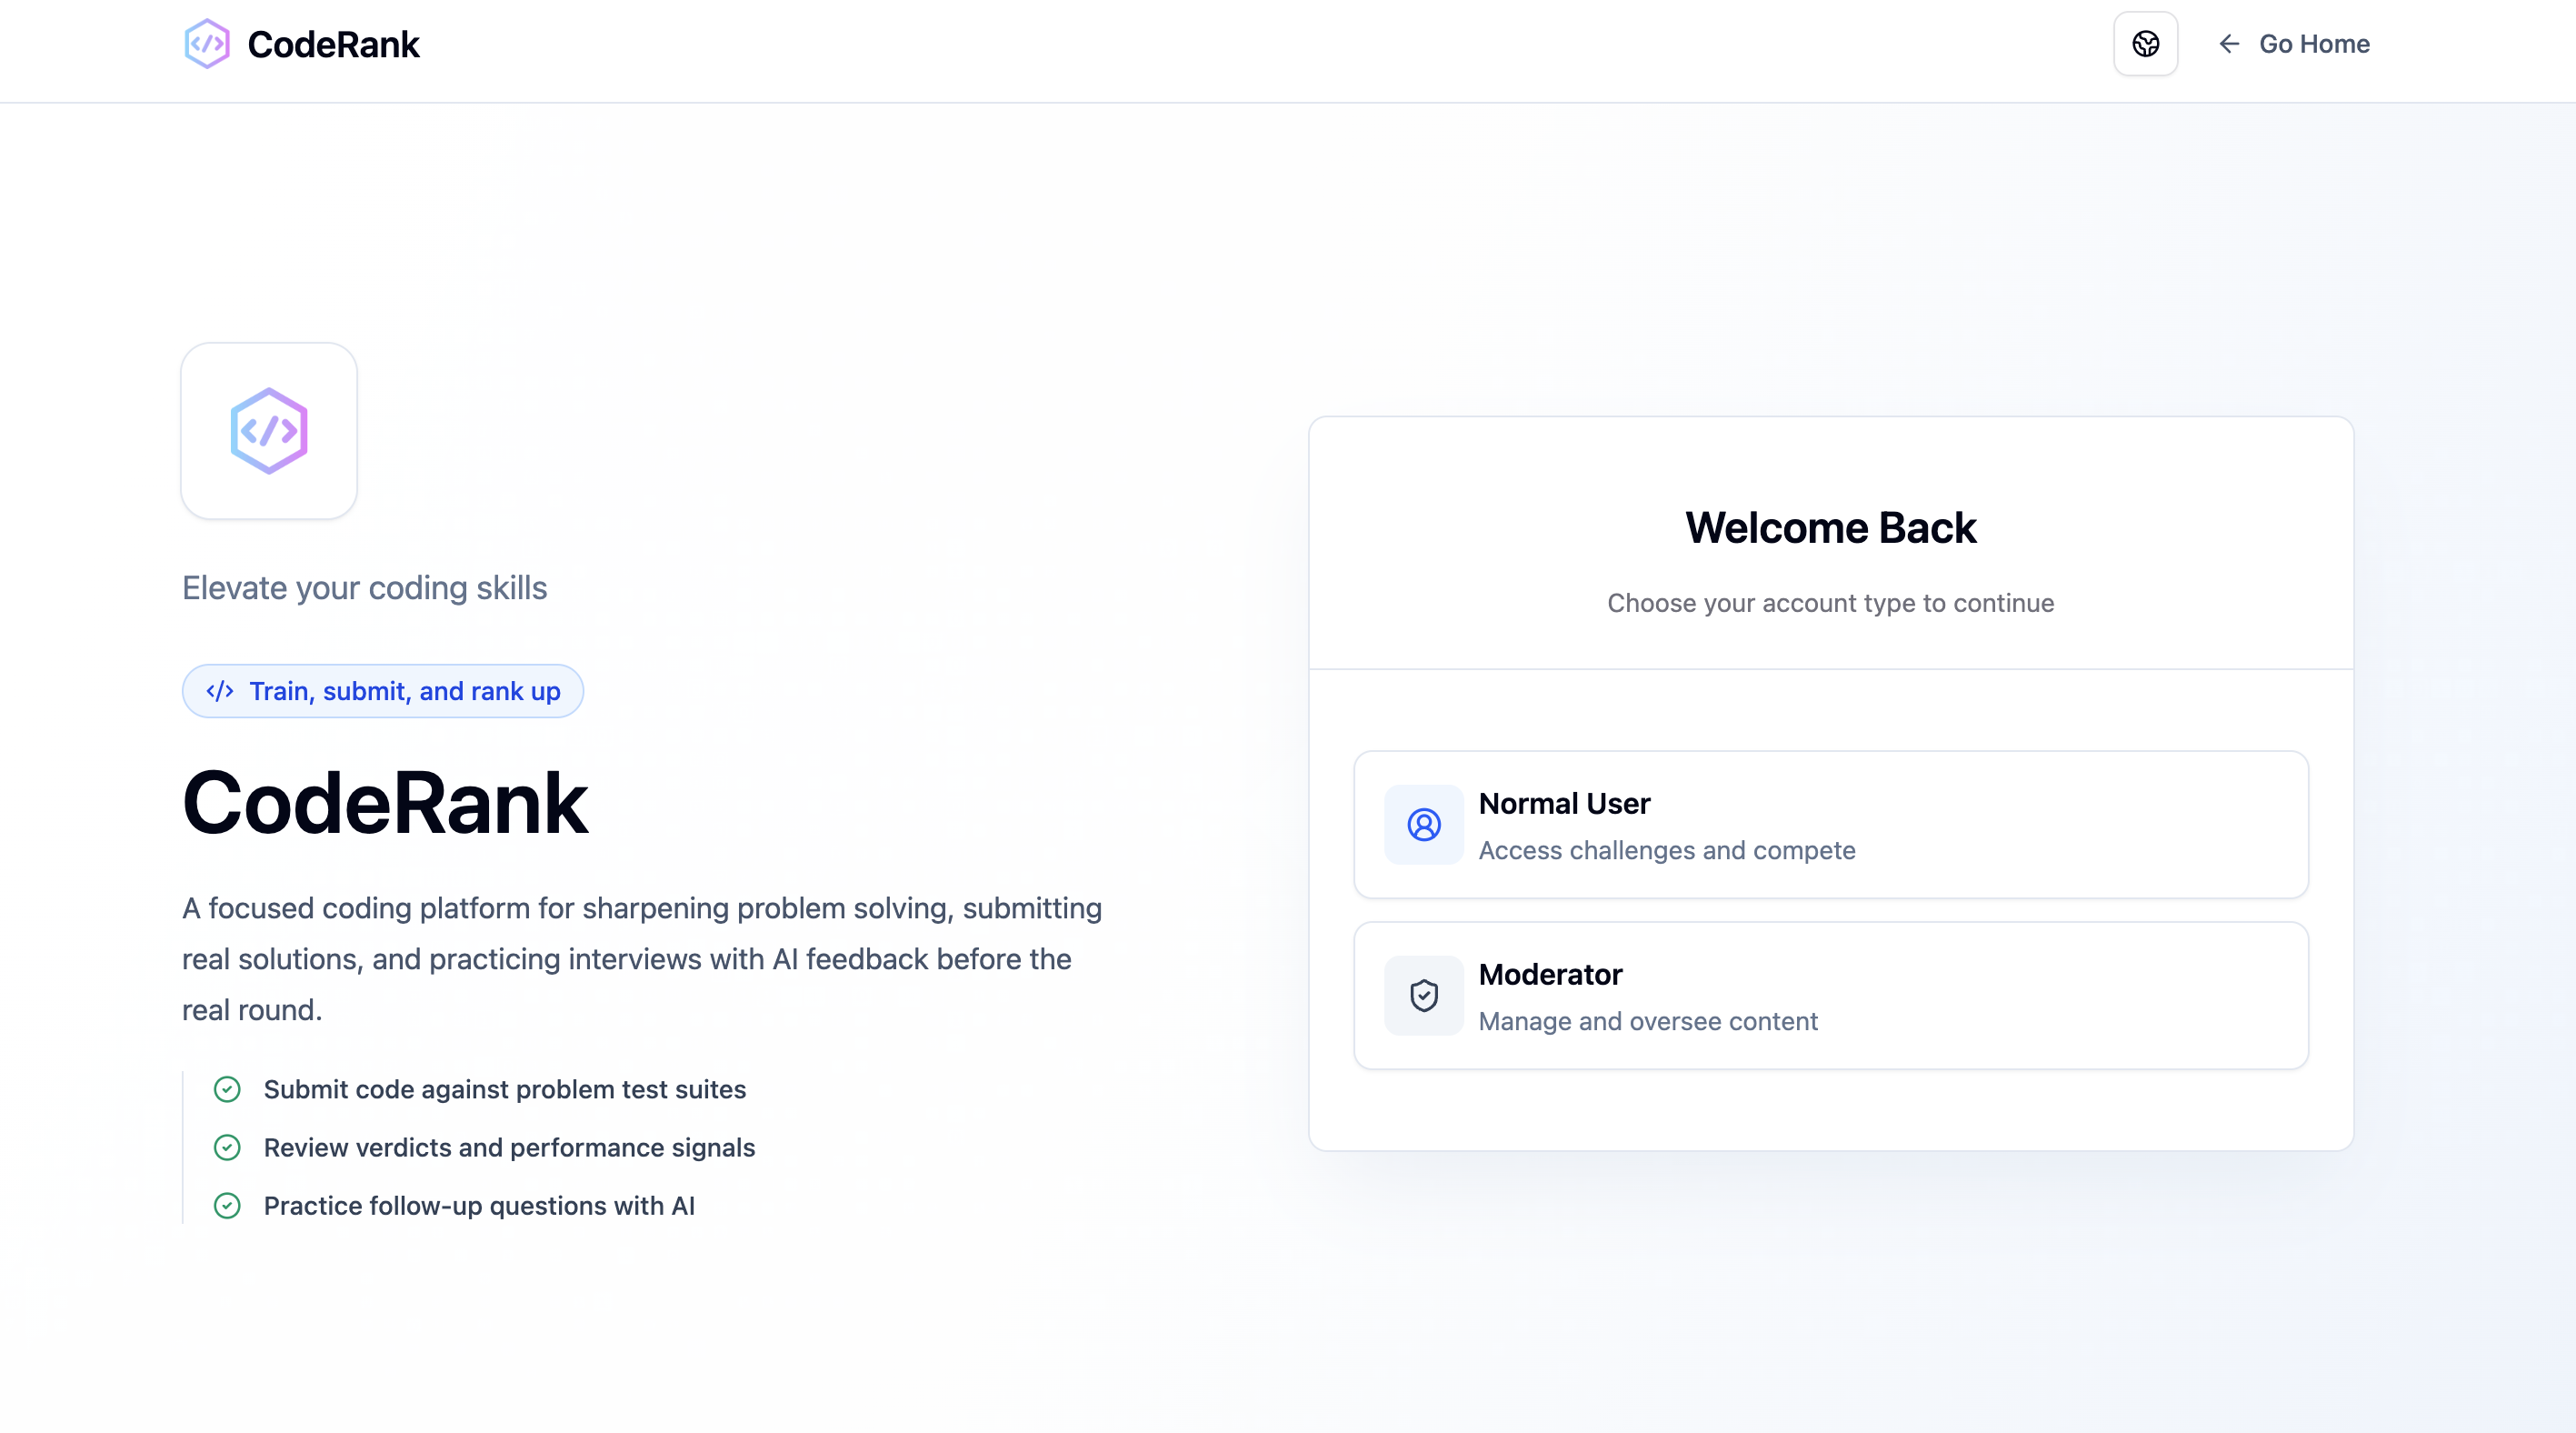
\includegraphics[width=1\textwidth]{Contents/Chapter 4/Mockup Design/Primary User/login_selection.png}
    \vspace{0.6cm}
    \caption{Login Page \- Role Selection}
\end{figure}

For Primary User, after selecting User login, the user will be directed to the User Login Page. This will include fields for entering username and password, along with a login button. There is also an option for login vie Google OAuth. After login successful, there will be a toast notification indicating success and redirecting to the Problem List page. Any validation errors will be displayed in the below of the corresponding input fields if the user enters incorrect credentials.
\begin{figure}[H]
    \centering
    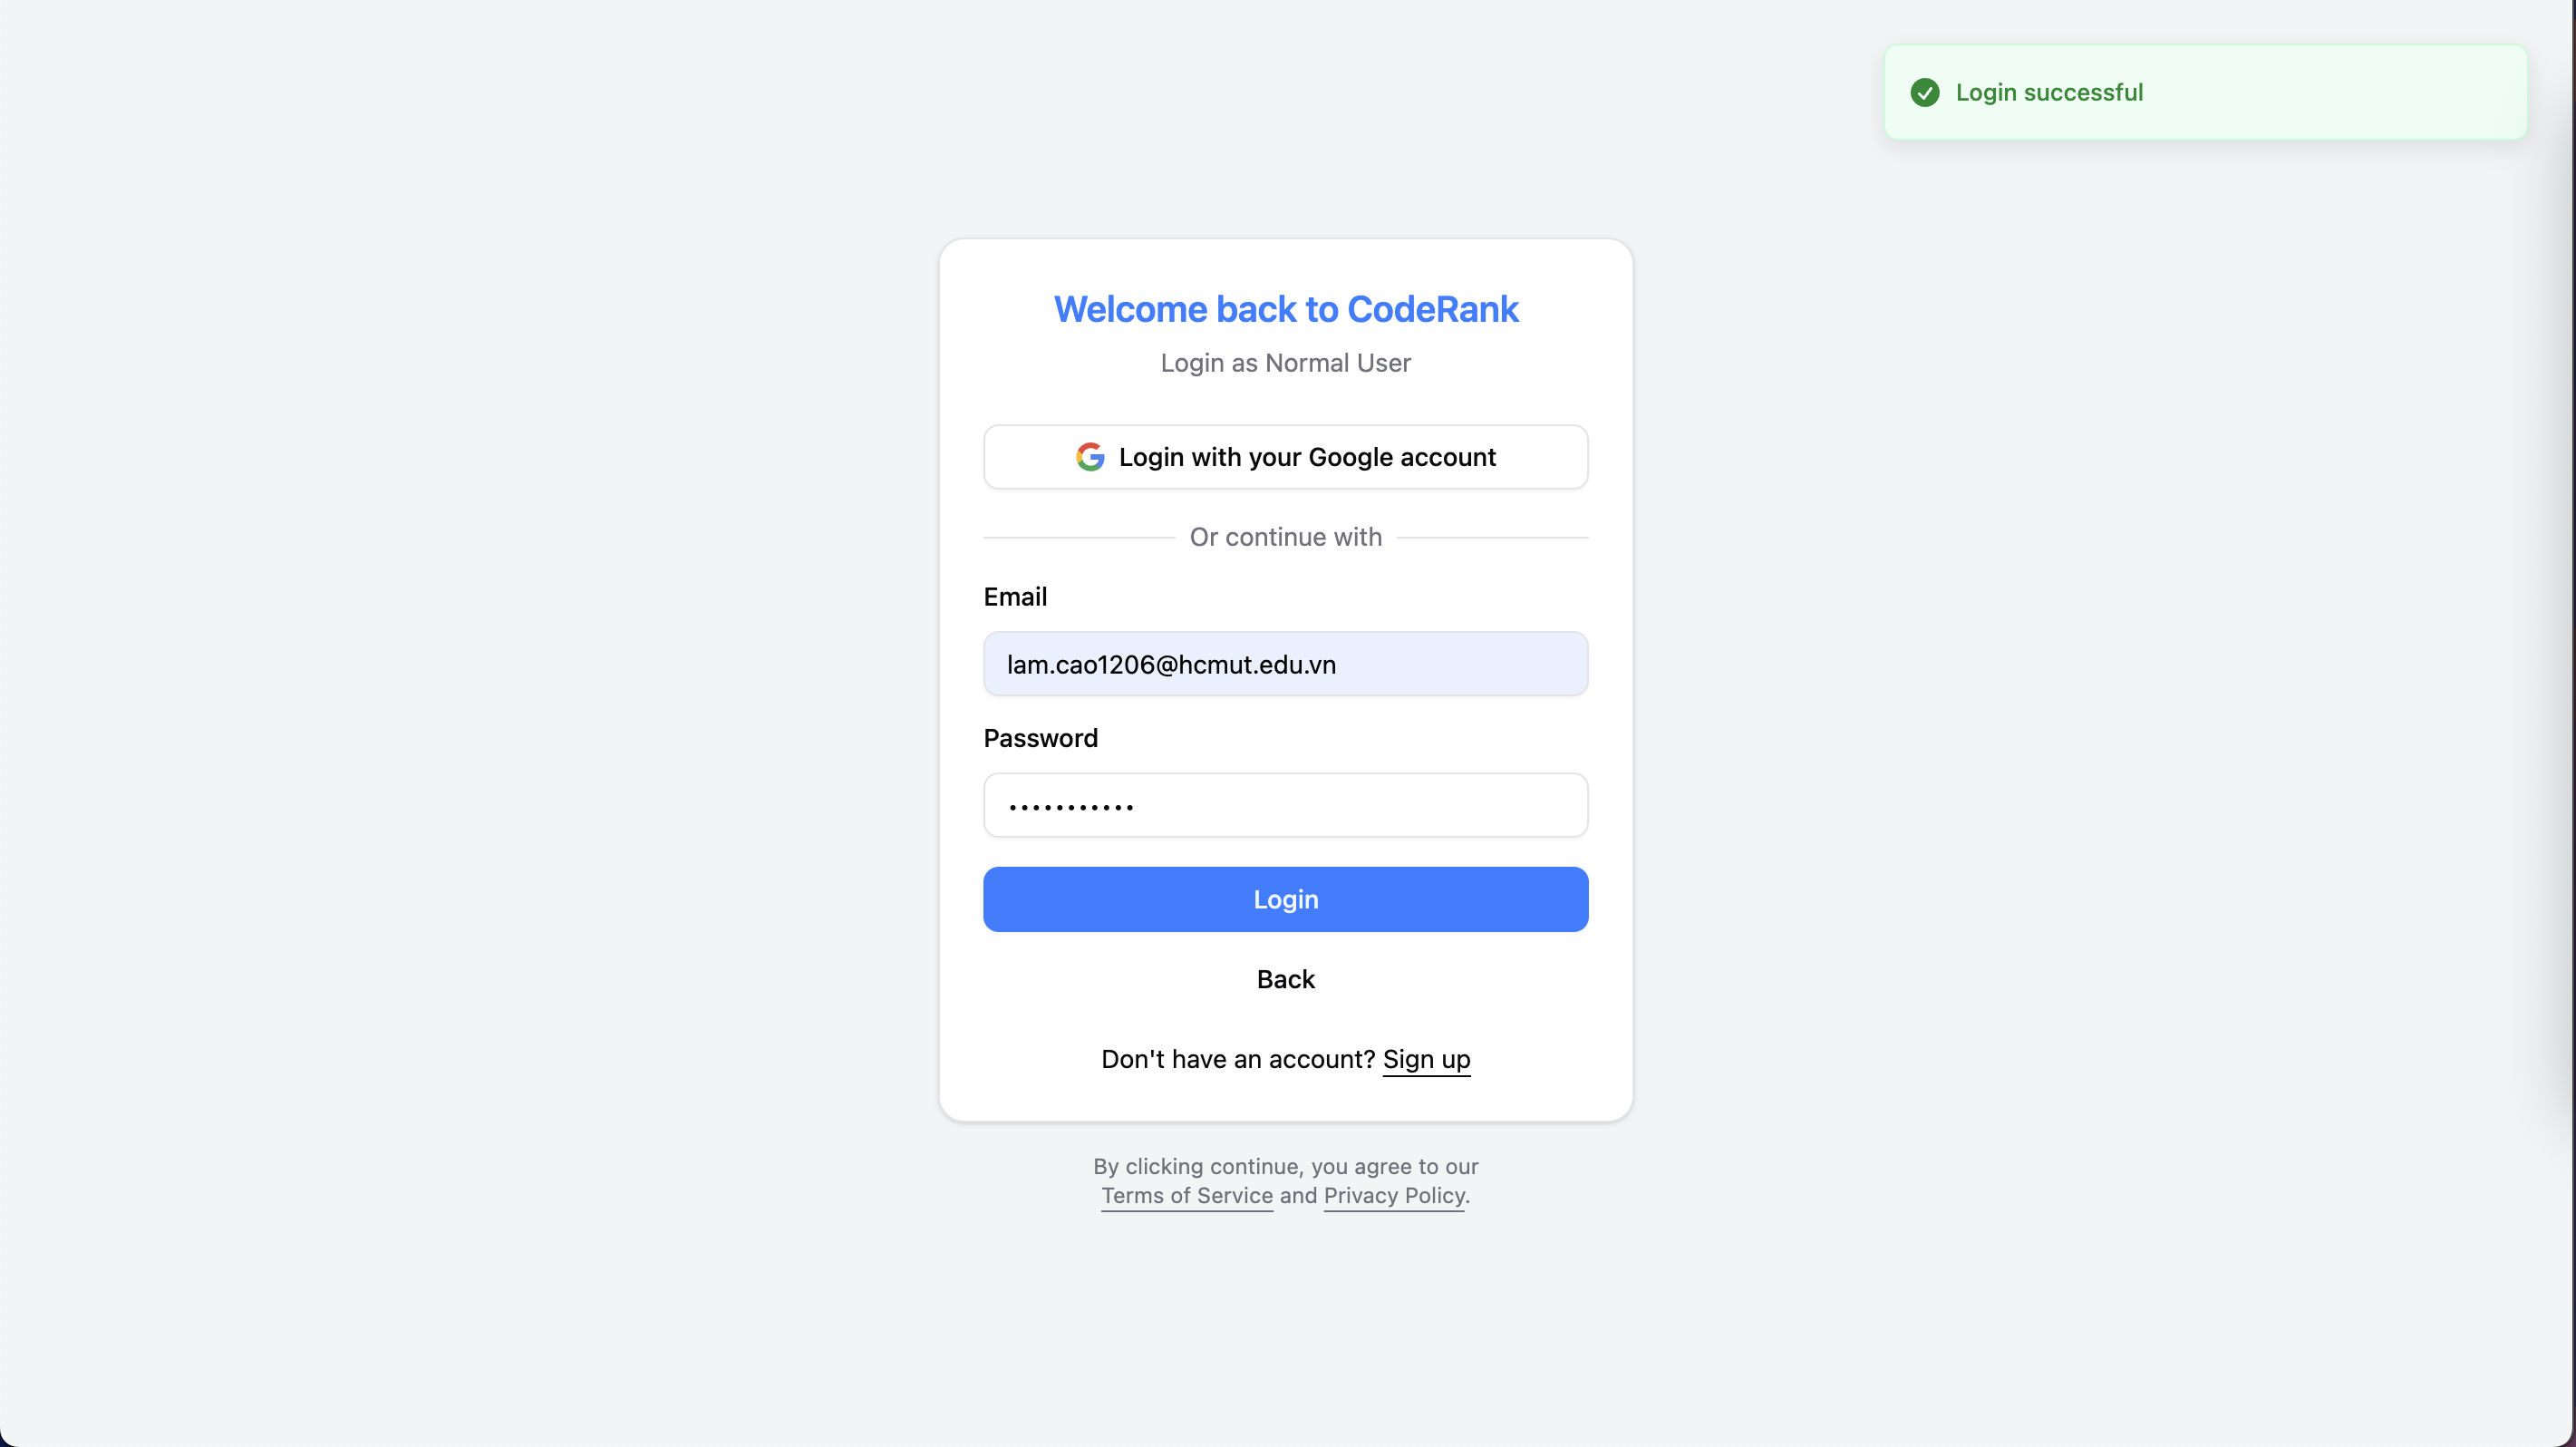
\includegraphics[width=1\textwidth]{Contents/Chapter 4/Mockup Design/Primary User/login_primary.png}
    \vspace{0.6cm}
    \caption{Login Page \- Primary User Login}
\end{figure}

\subsubsubsection*{Problem List}
After logging in, the Primary User will be directed to the Problem List page. This page displays a list of coding problems available on the platform, along with relevant details such as problem title, difficulty level, and tags. Users can filter and sort the problems based on various criteria to find specific challenges they want to solve.
\begin{figure}[H]
    \centering
    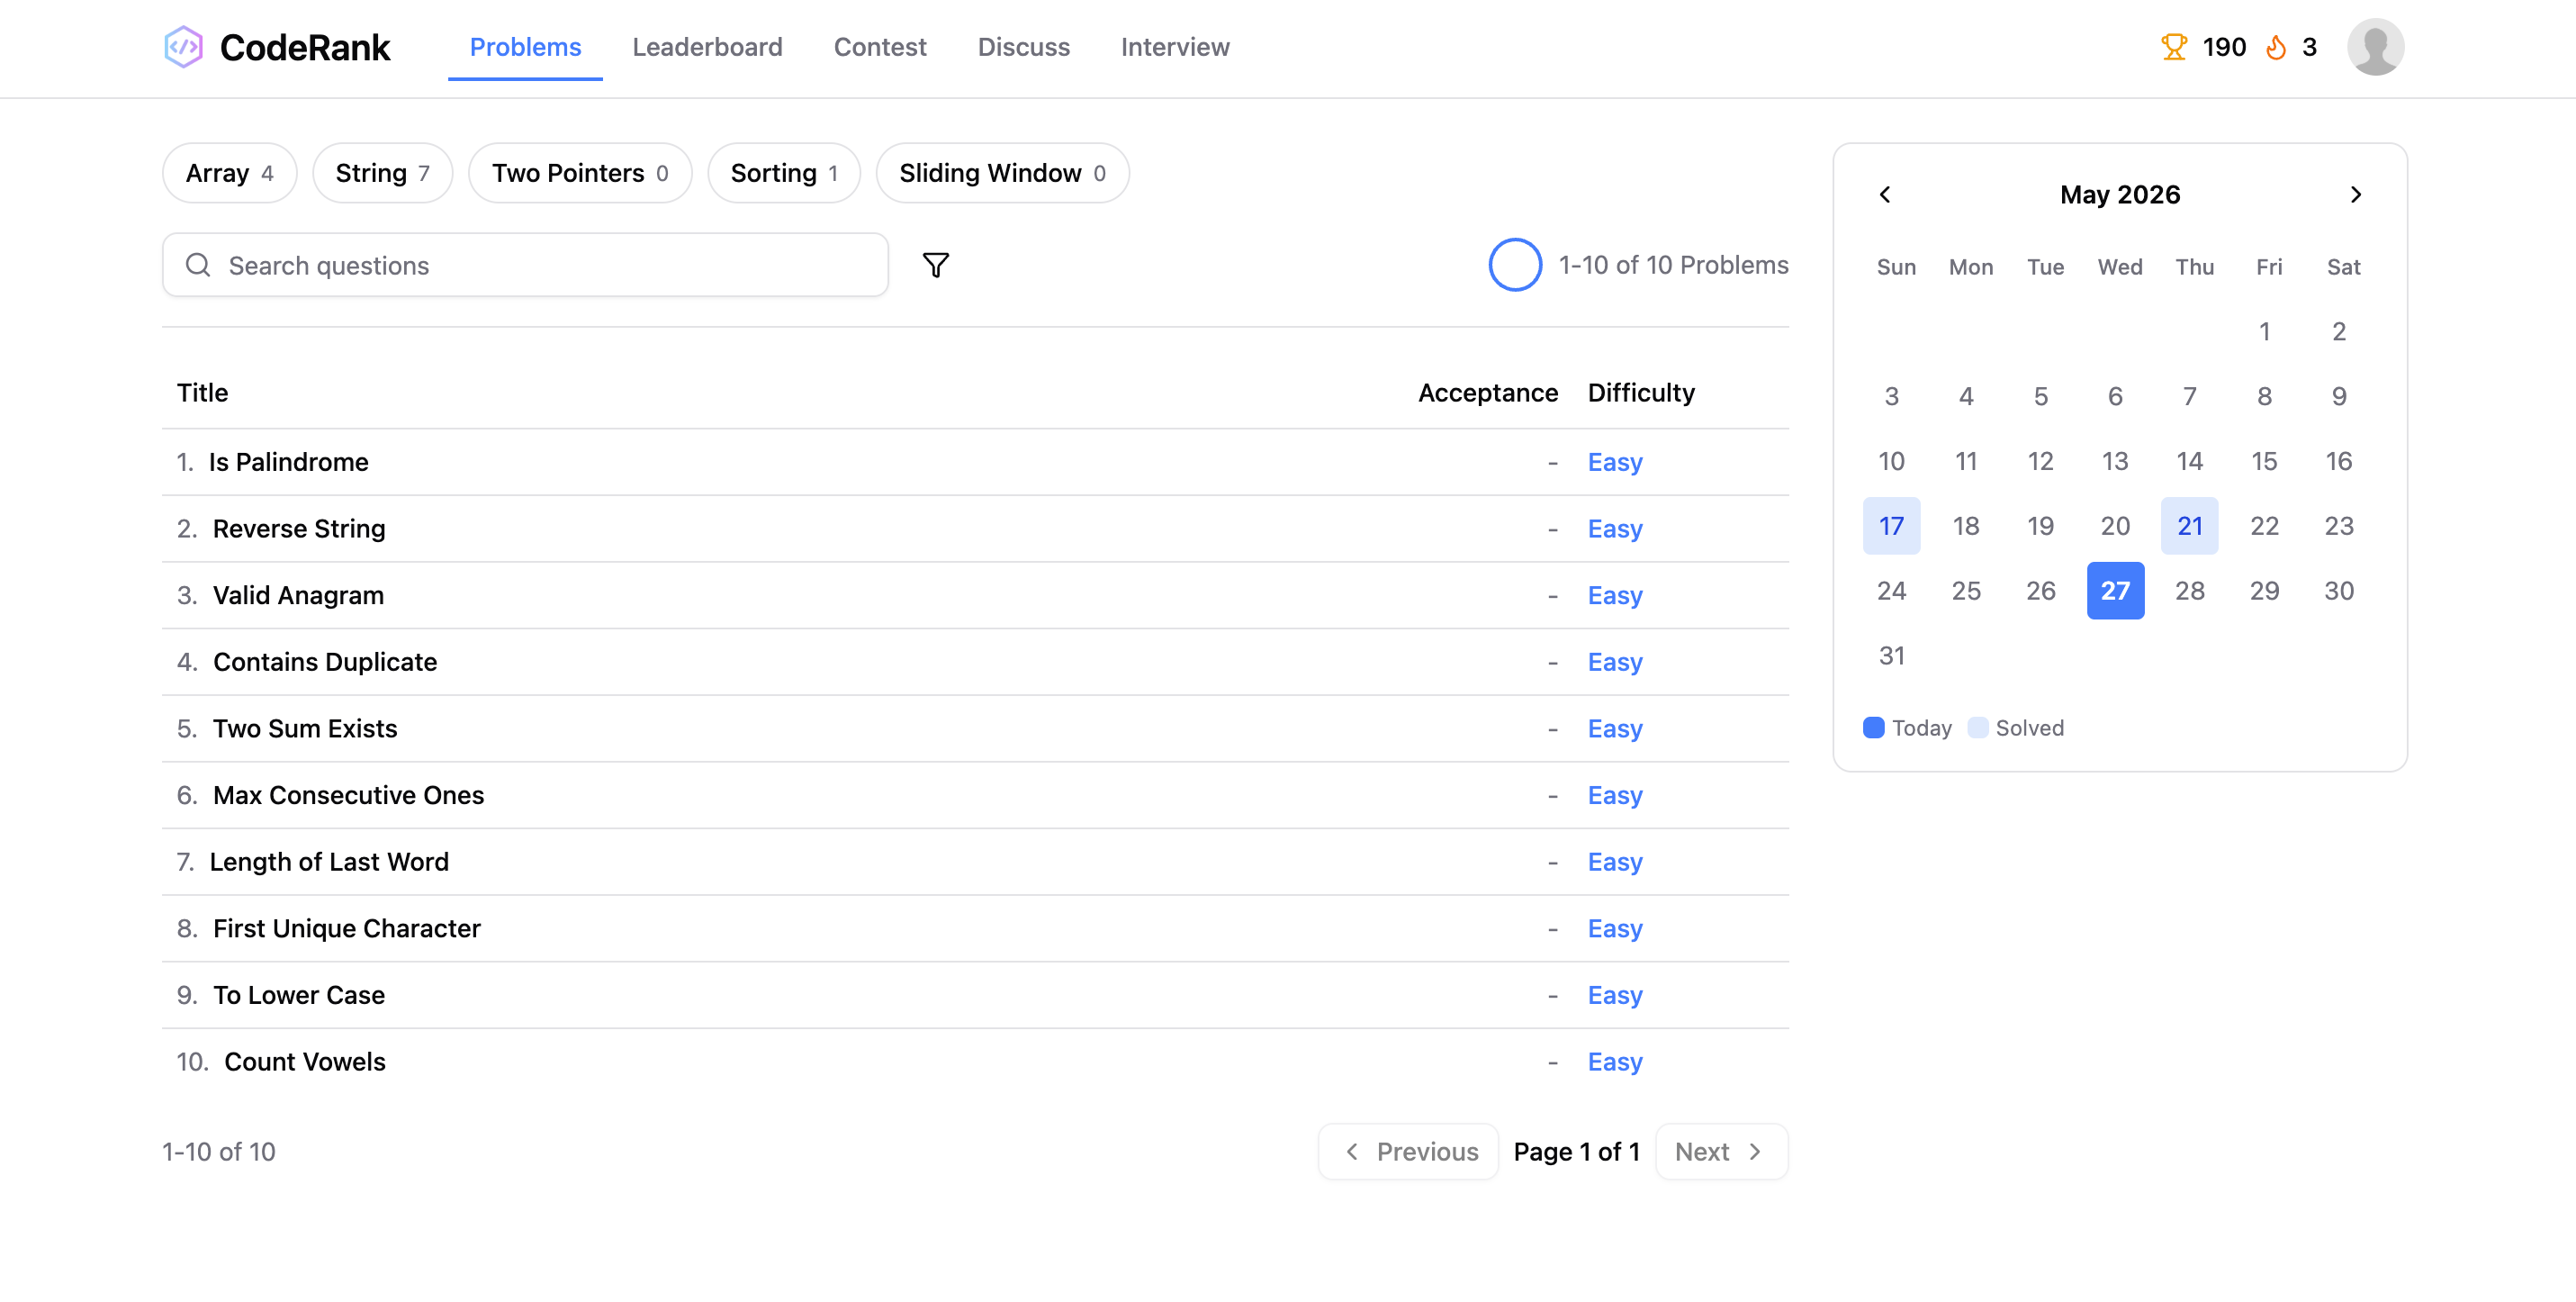
\includegraphics[width=1\textwidth]{Contents/Chapter 4/Mockup Design/Primary User/problem_list.png}
    \vspace{0.6cm}
    \caption{Problem List page}
\end{figure}

The Problem List page also includes a search bar at the top, allowing users to quickly search for problems by keywords or tags. Each problem entry in the list is clickable, leading to the Problem Detail page where users can view the full problem description and submit their solutions.
\begin{figure}[H]
    \centering
    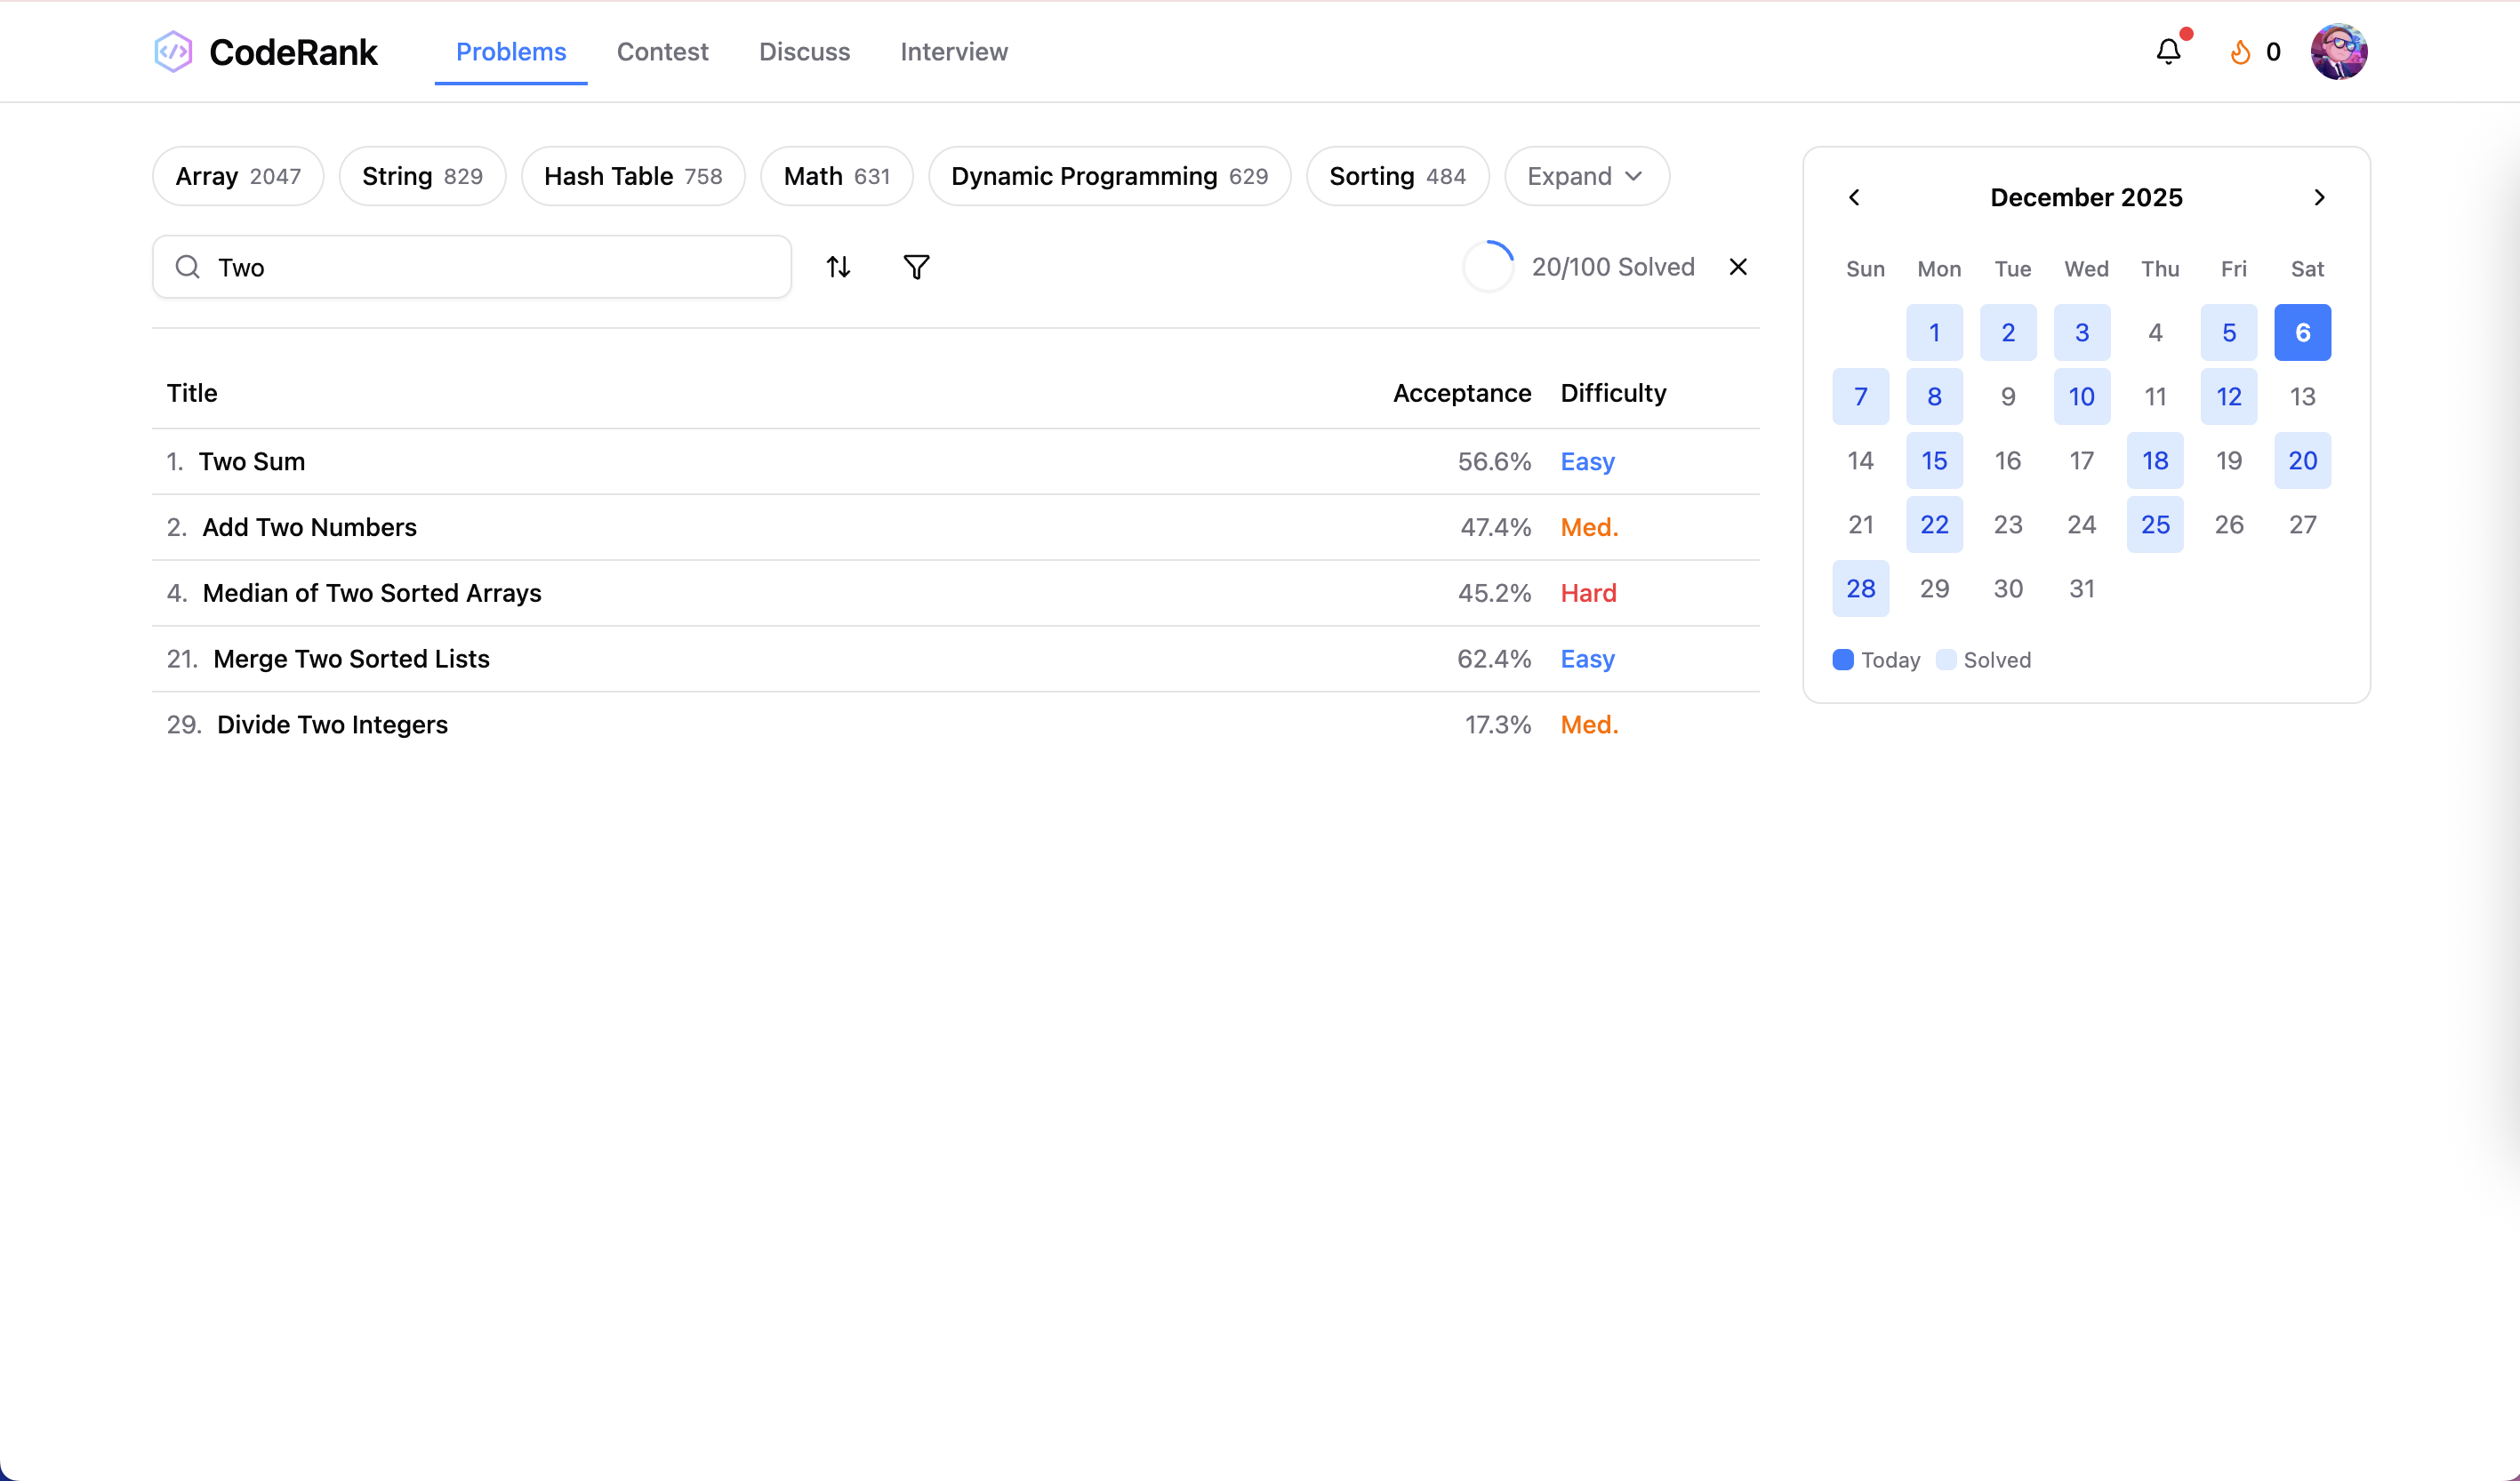
\includegraphics[width=1\textwidth]{Contents/Chapter 4/Mockup Design/Primary User/problem_list_search.png}
    \vspace{0.6cm}
    \caption{Problem List Search}
\end{figure}

In order to solve a problem, the user can click on the problem title in the Problem List. This will take them to the Problem Detail page, where they can read the problem description, view constraints, and submit their code solution.
\begin{figure}[H]
    \centering
    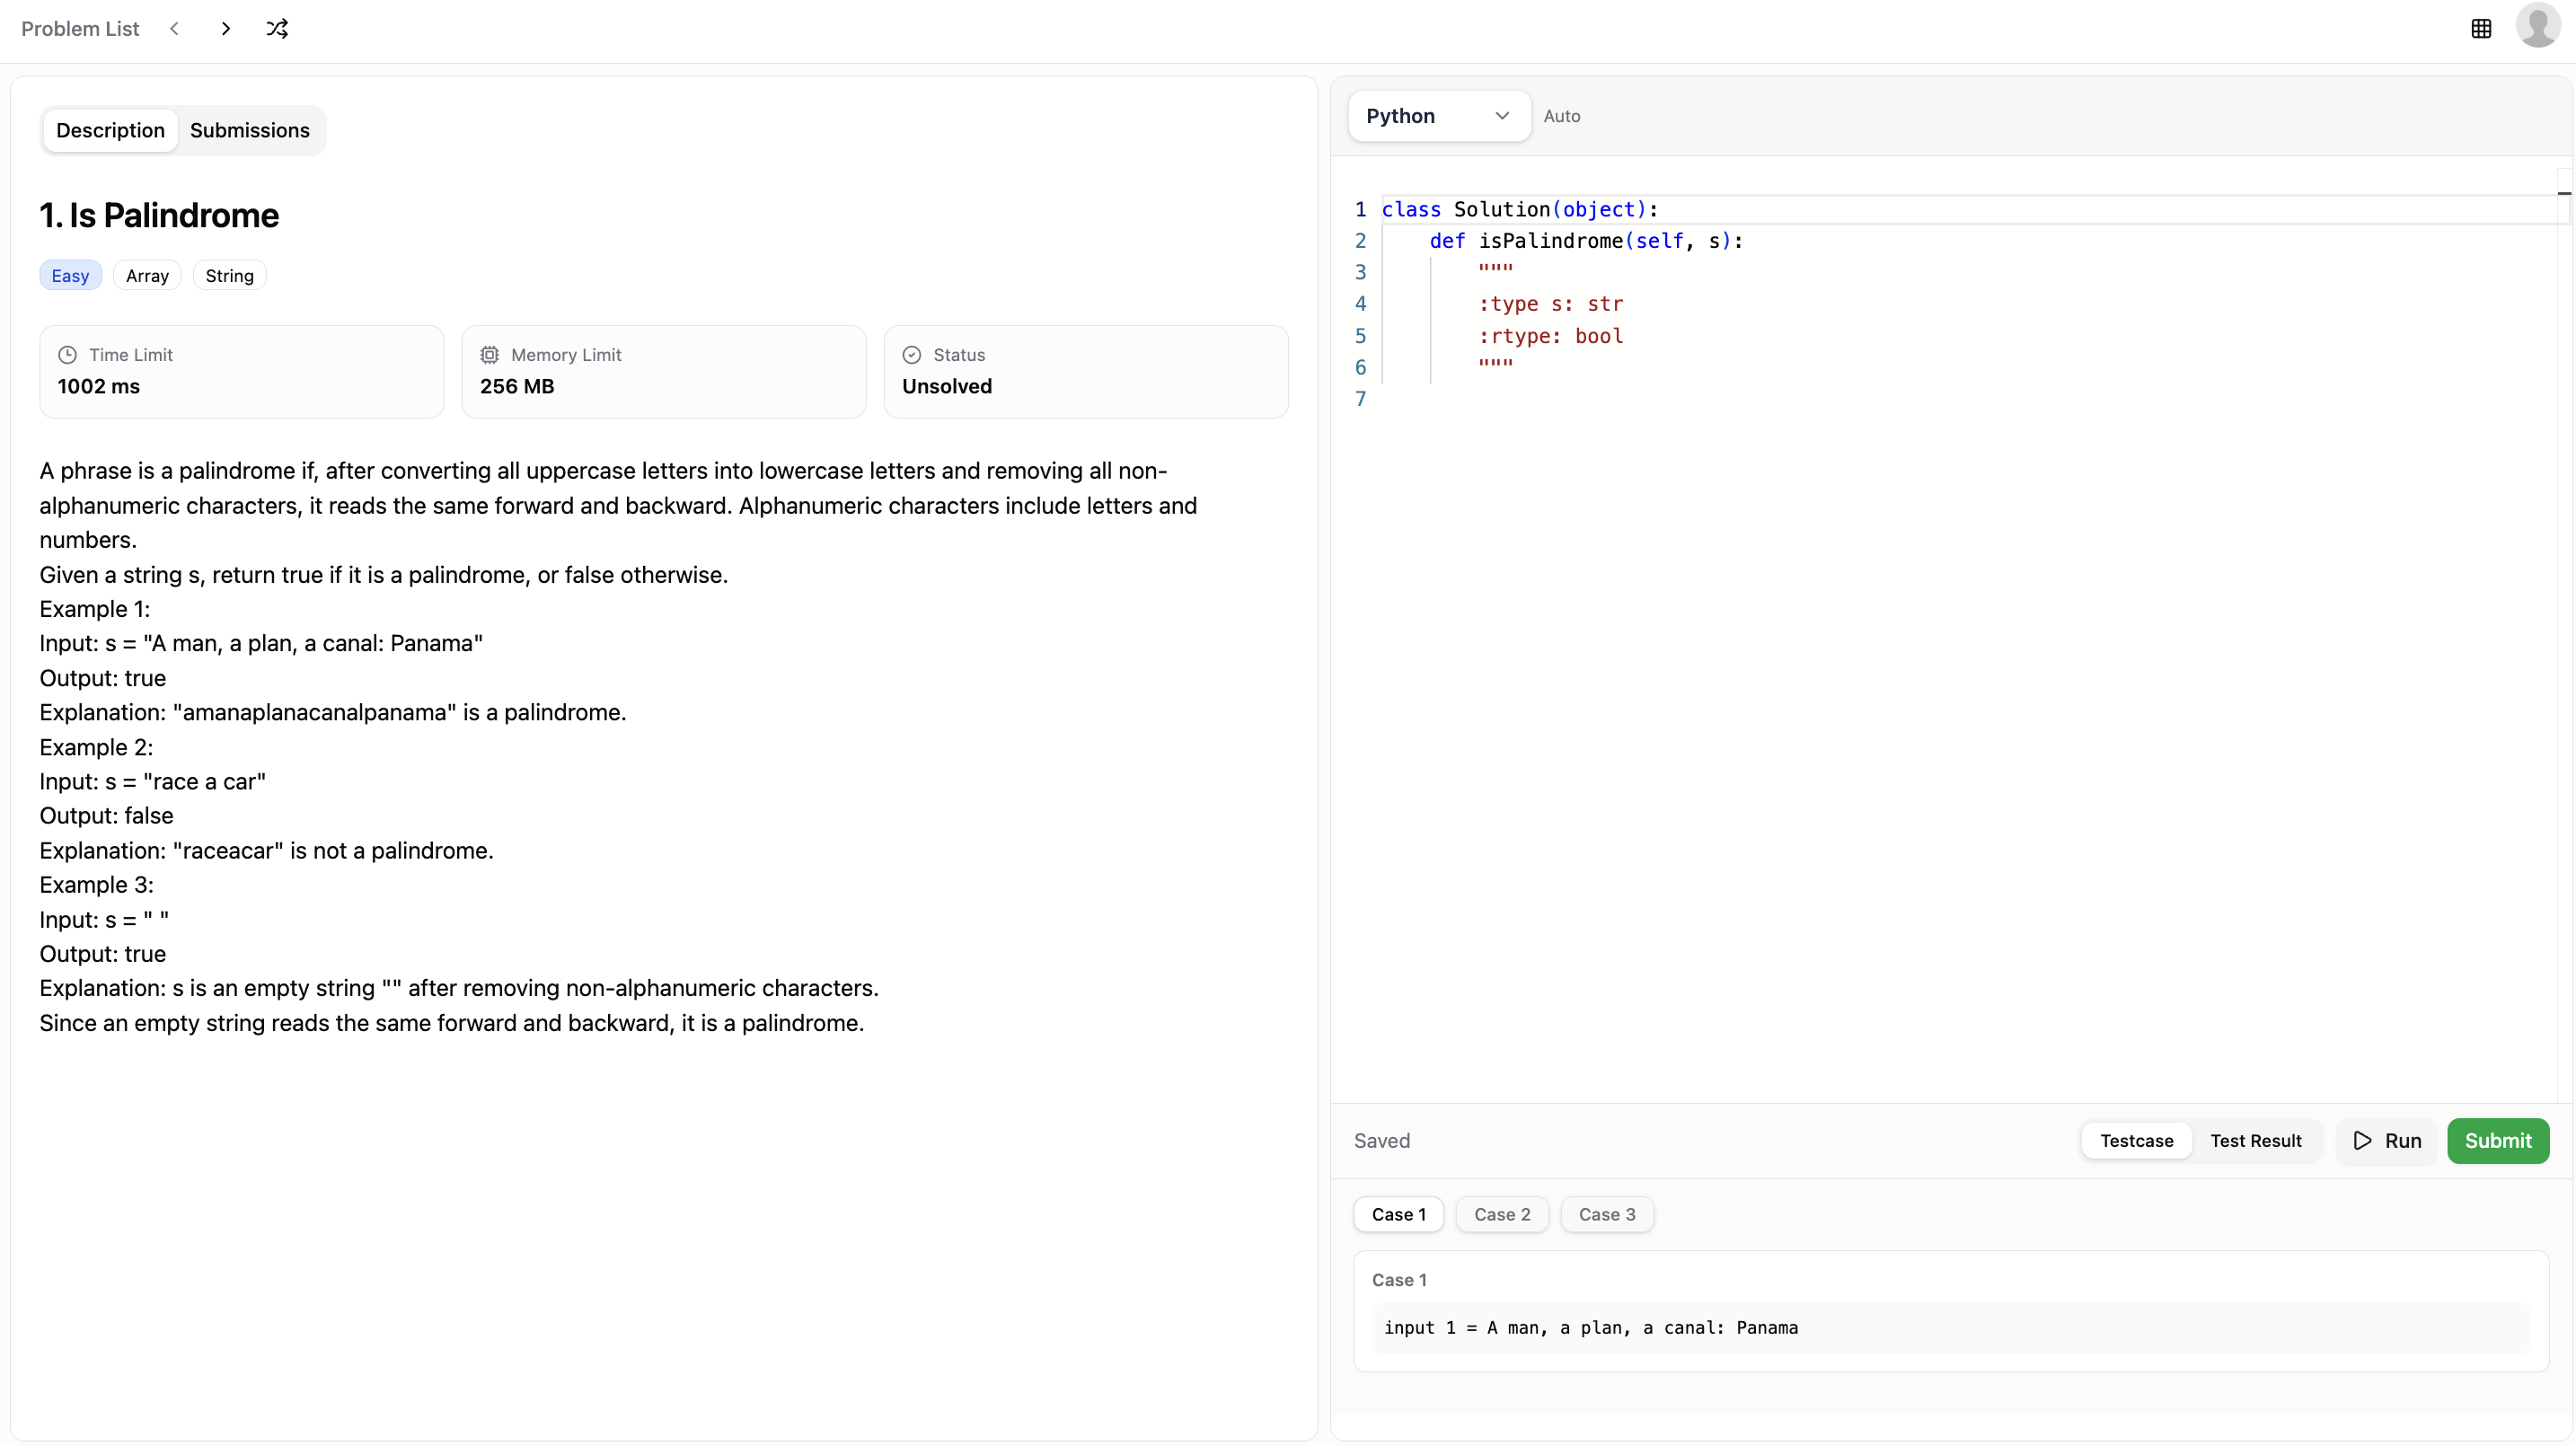
\includegraphics[width=1\textwidth]{Contents/Chapter 4/Mockup Design/Primary User/problem_detail.png}
    \vspace{0.6cm}
    \caption{Problem Detail page}
\end{figure}


\subsubsection*{Discussion}

Beside solving problems, primary user can access the Discussion feature from the main navigation menu after logging in. The Discussion feature allows users to engage in conversations related to coding problems, share insights, ask questions, and collaborate with other users.

\begin{figure}[H]
    \centering
    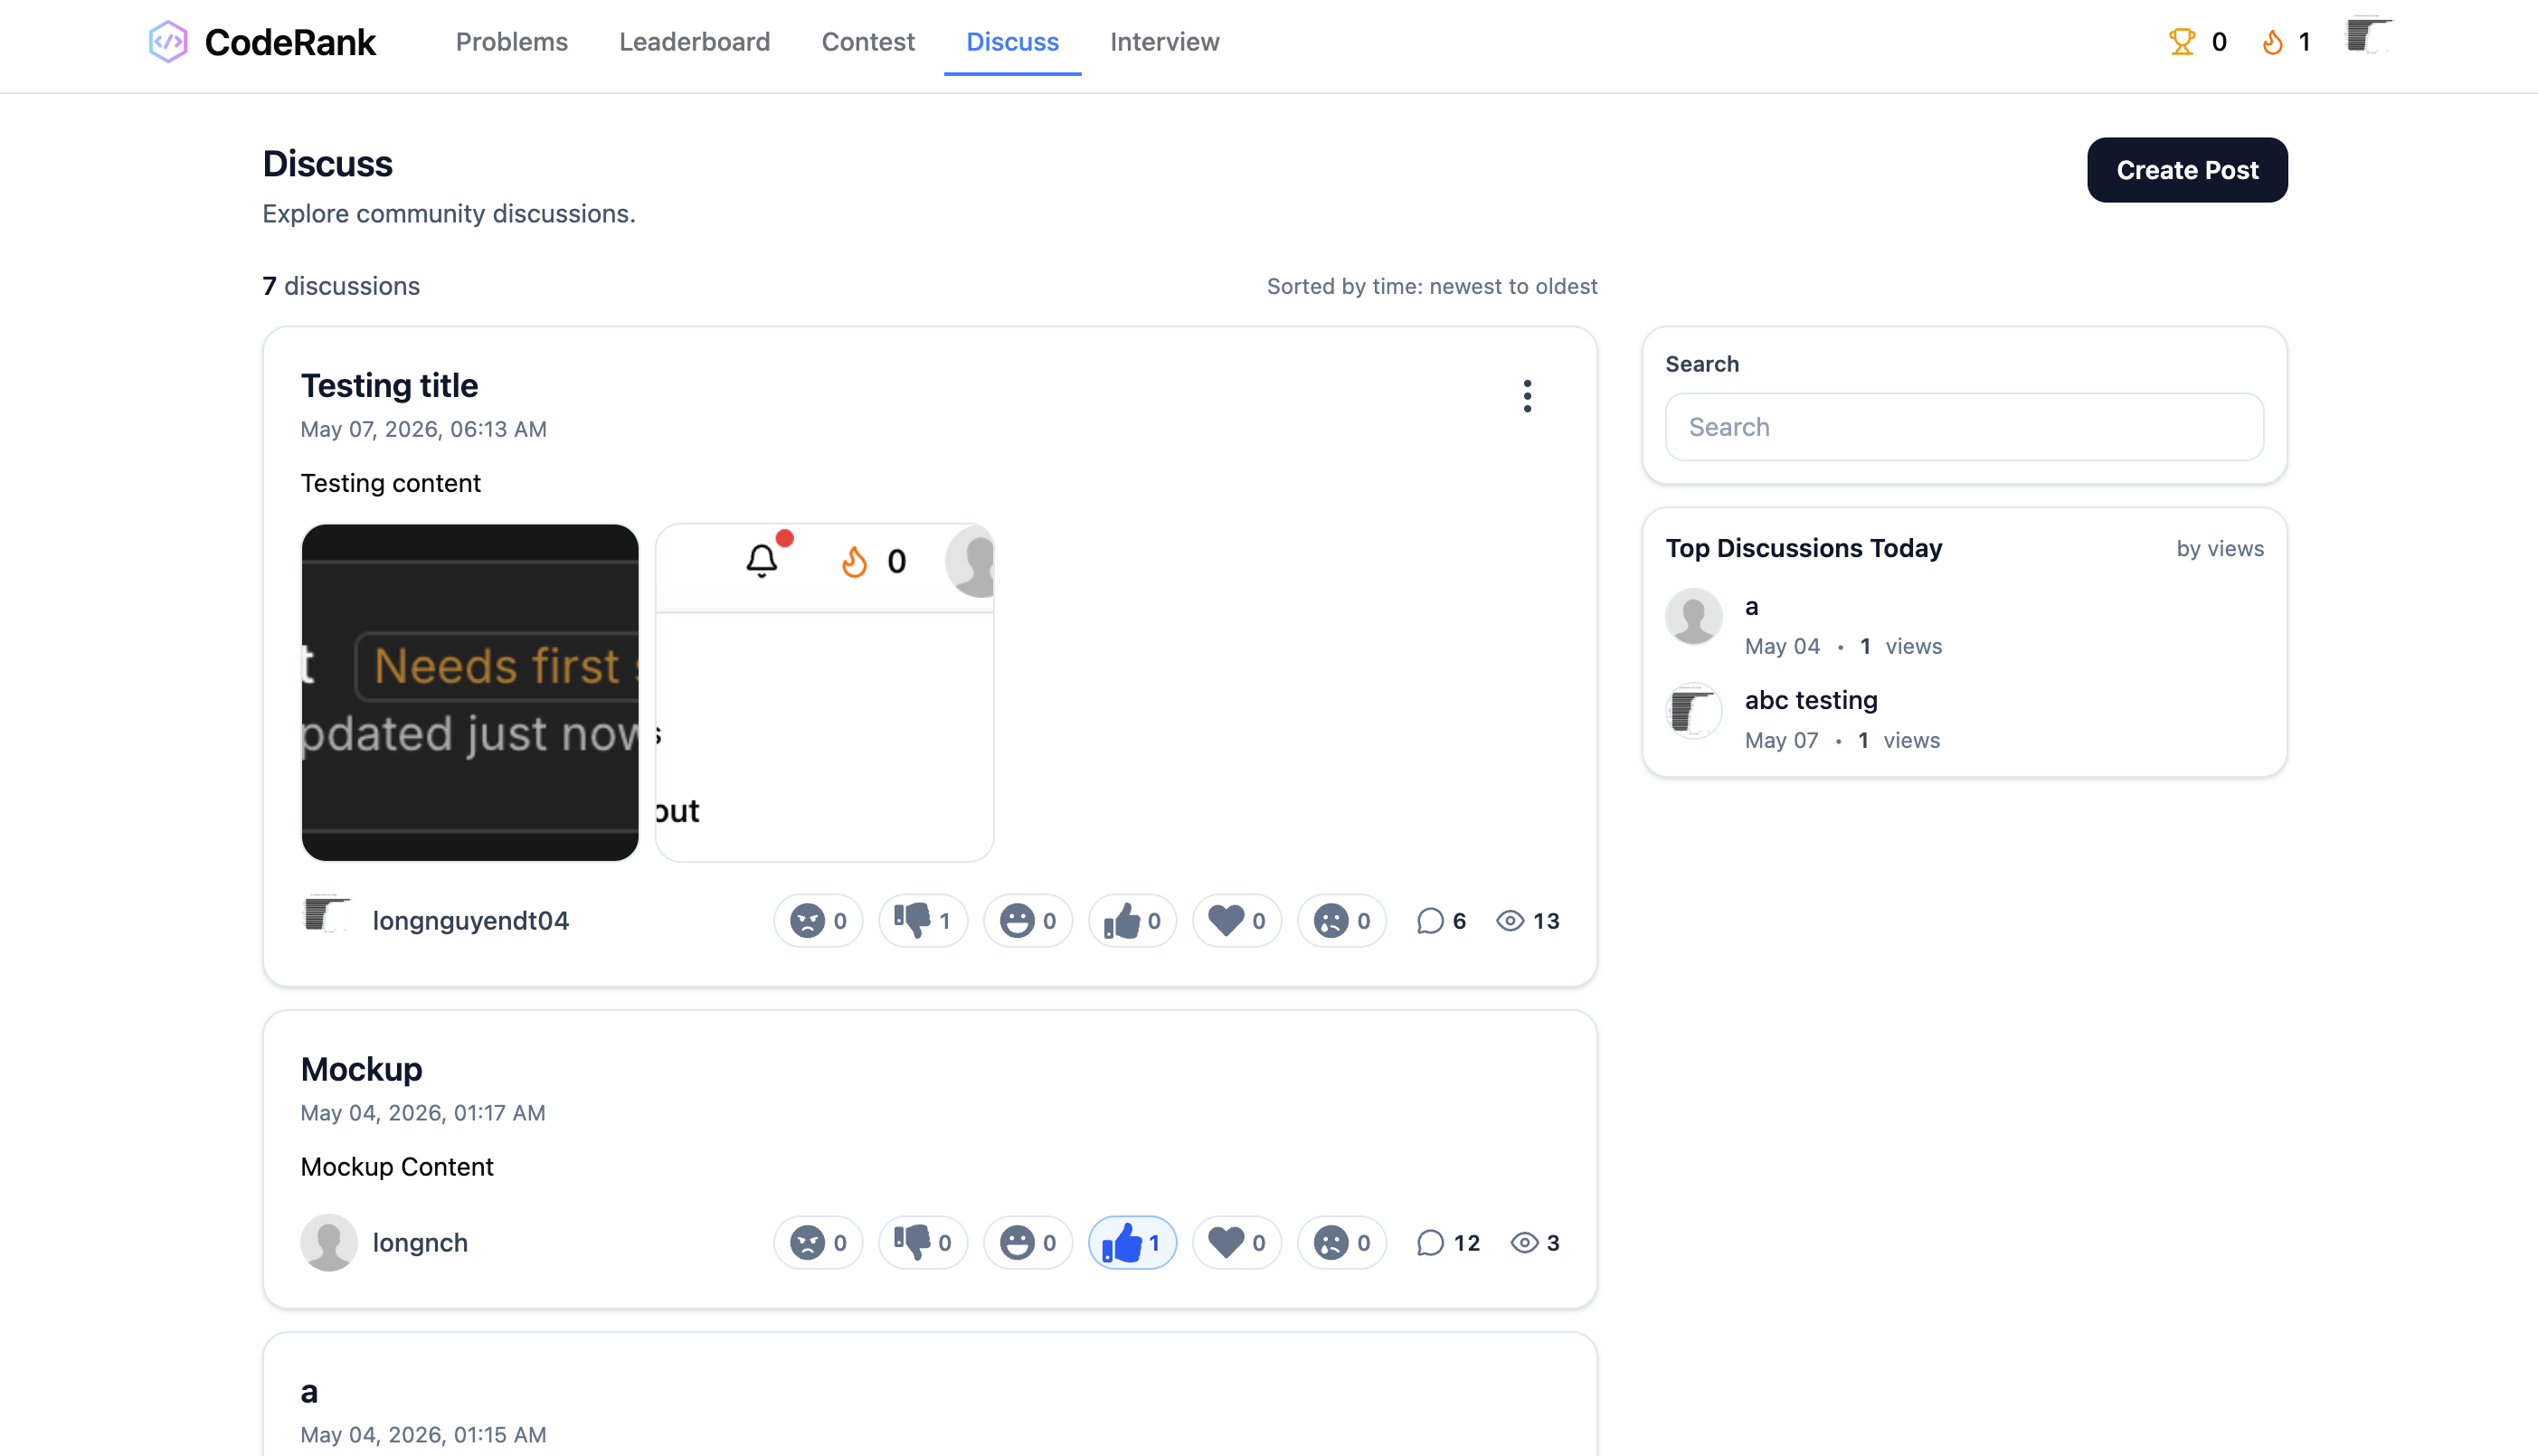
\includegraphics[width=1\textwidth]{Contents/Chapter 4/Mockup Design/Primary User/discussion-1.png}
    \vspace{0.6cm}
    \caption{Discussion List}
\end{figure}

In order to join a discussion, the user can select a specific discussion thread from the Discussion List. This will take them to the Discussion Detail page, where they can view all messages within that thread and participate in the conversation by posting their own messages.
\begin{figure}[H]
    \centering
    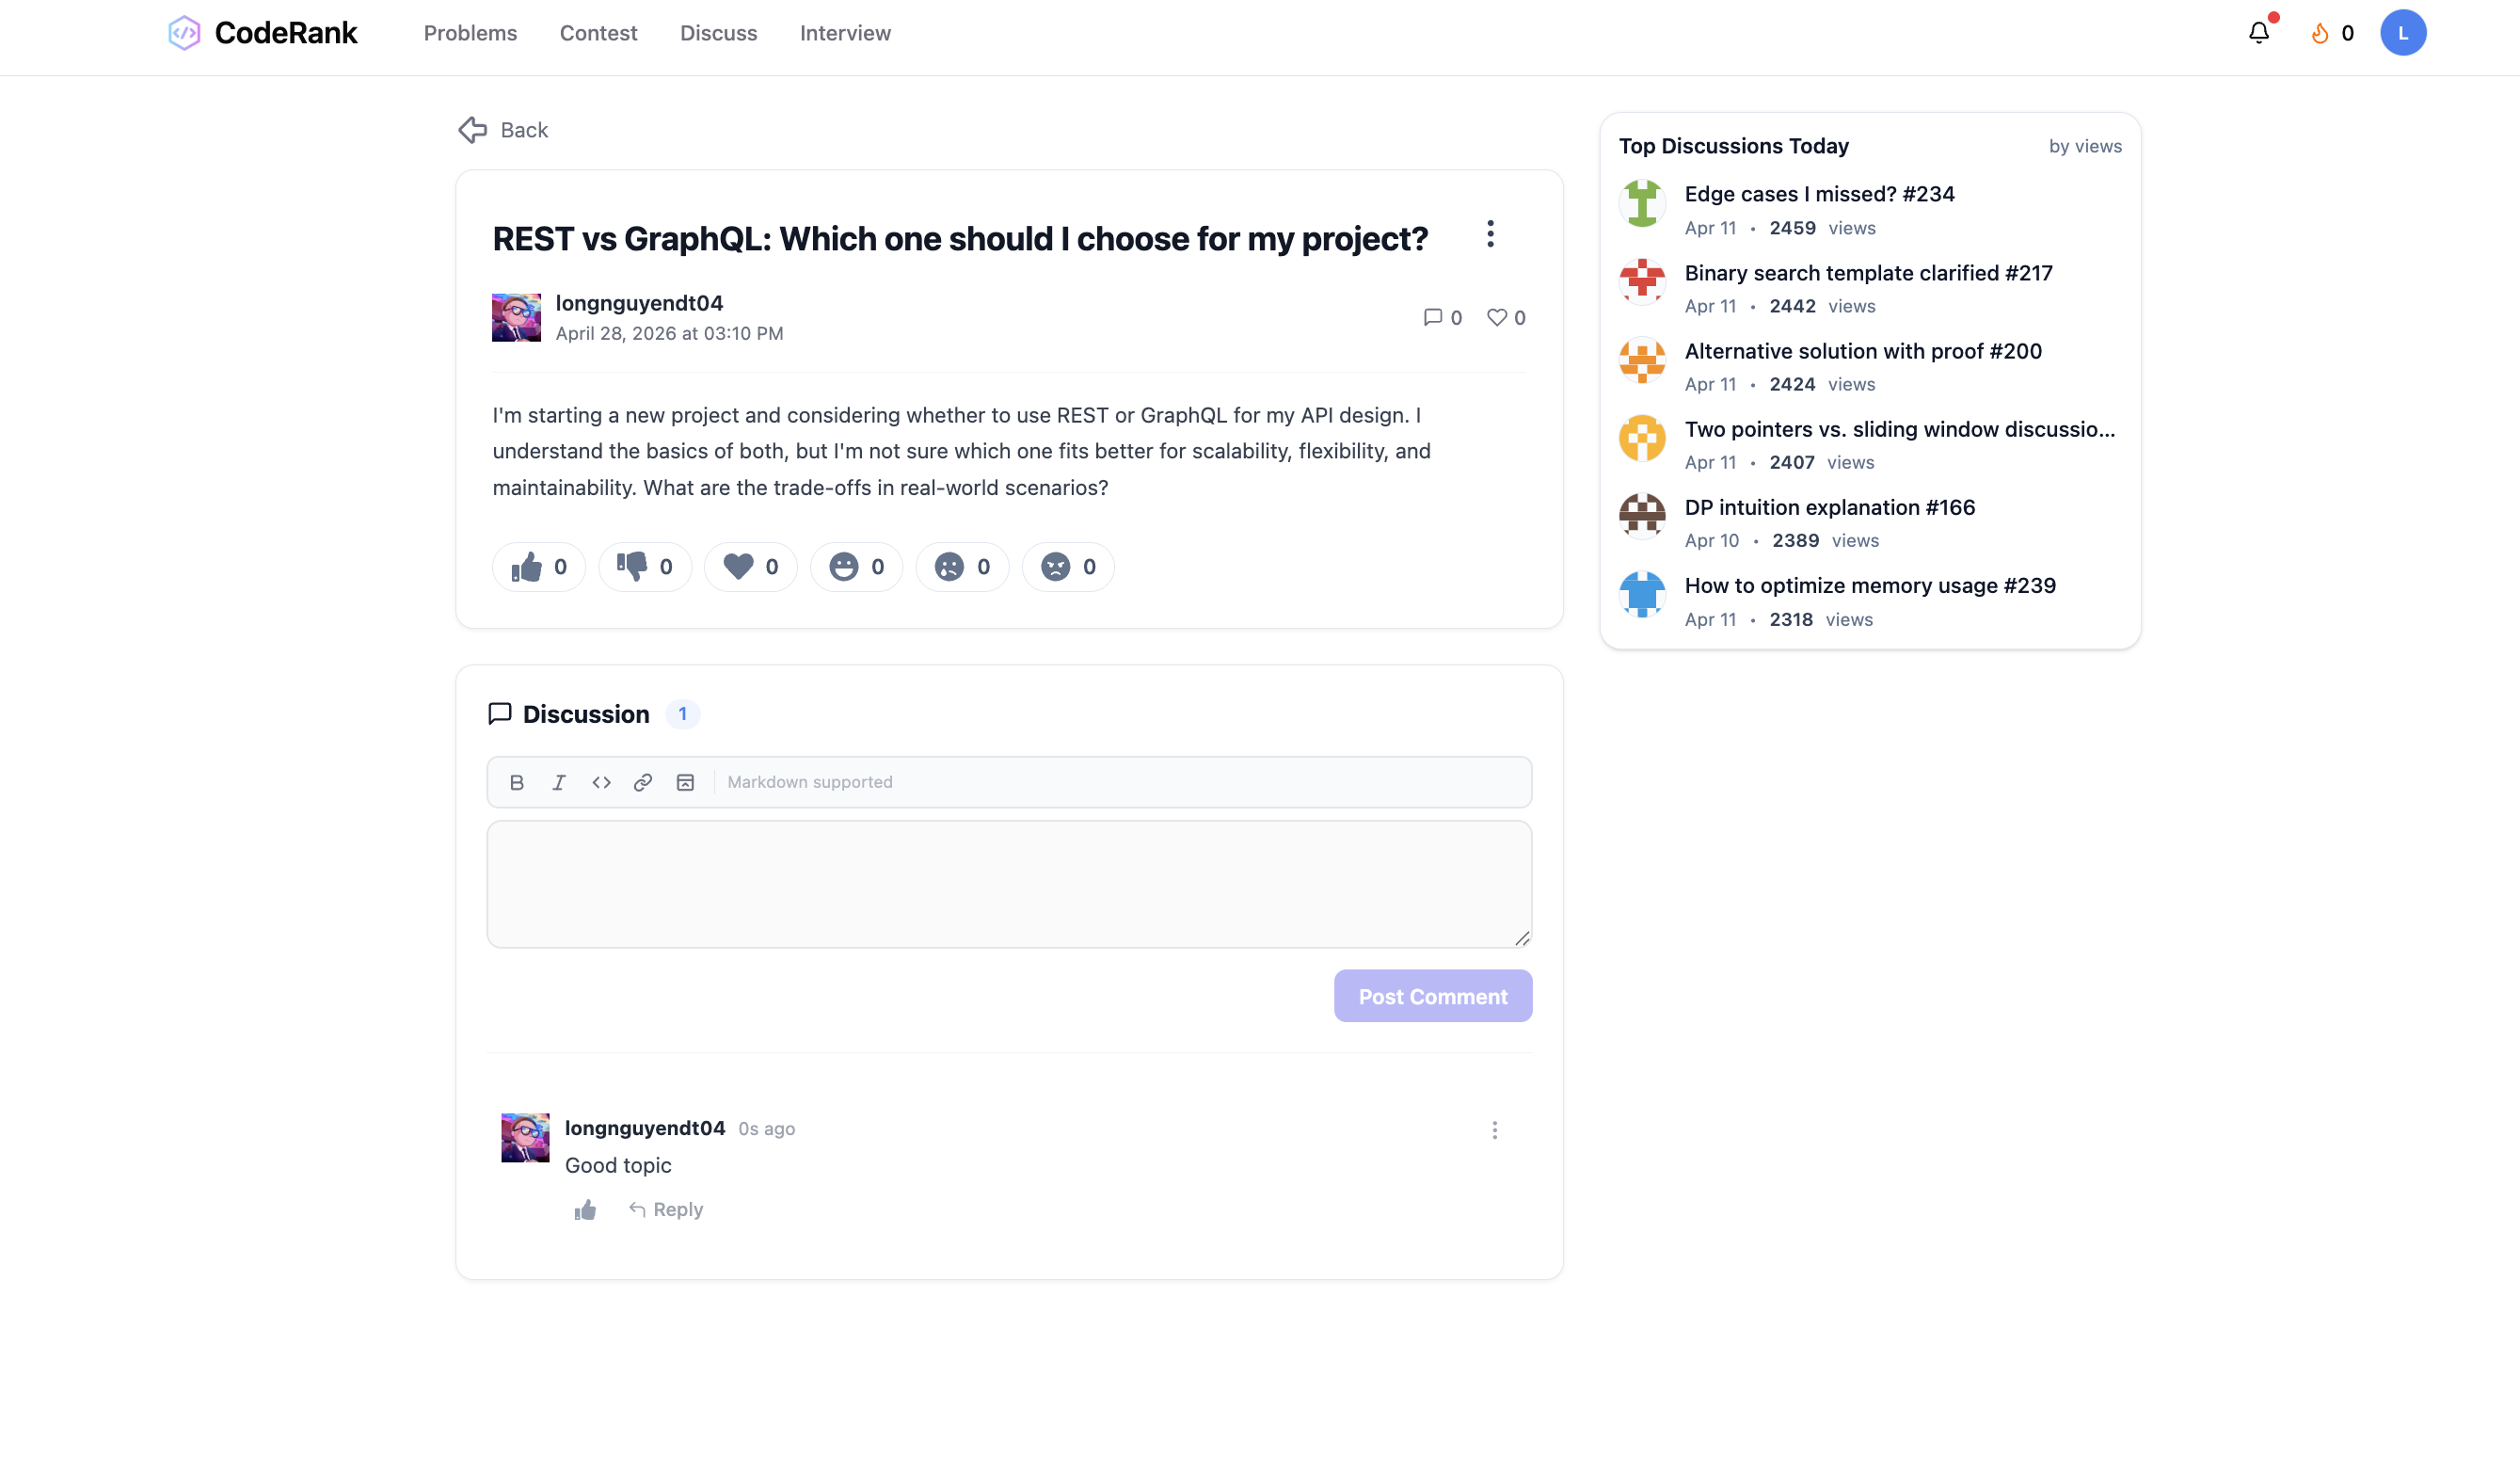
\includegraphics[width=1\textwidth]{Contents/Chapter 4/Mockup Design/Primary User/discussion-3.png}
    \vspace{0.6cm}
    \caption{Discussion Detail}
\end{figure}

To create a new discussion thread, the user can click in the button \textbf{Create} in the discussion list page. Here, they can enter a title, choose topic, tags, and write the initial message to start the discussion.

\begin{figure}[H]
    \centering
    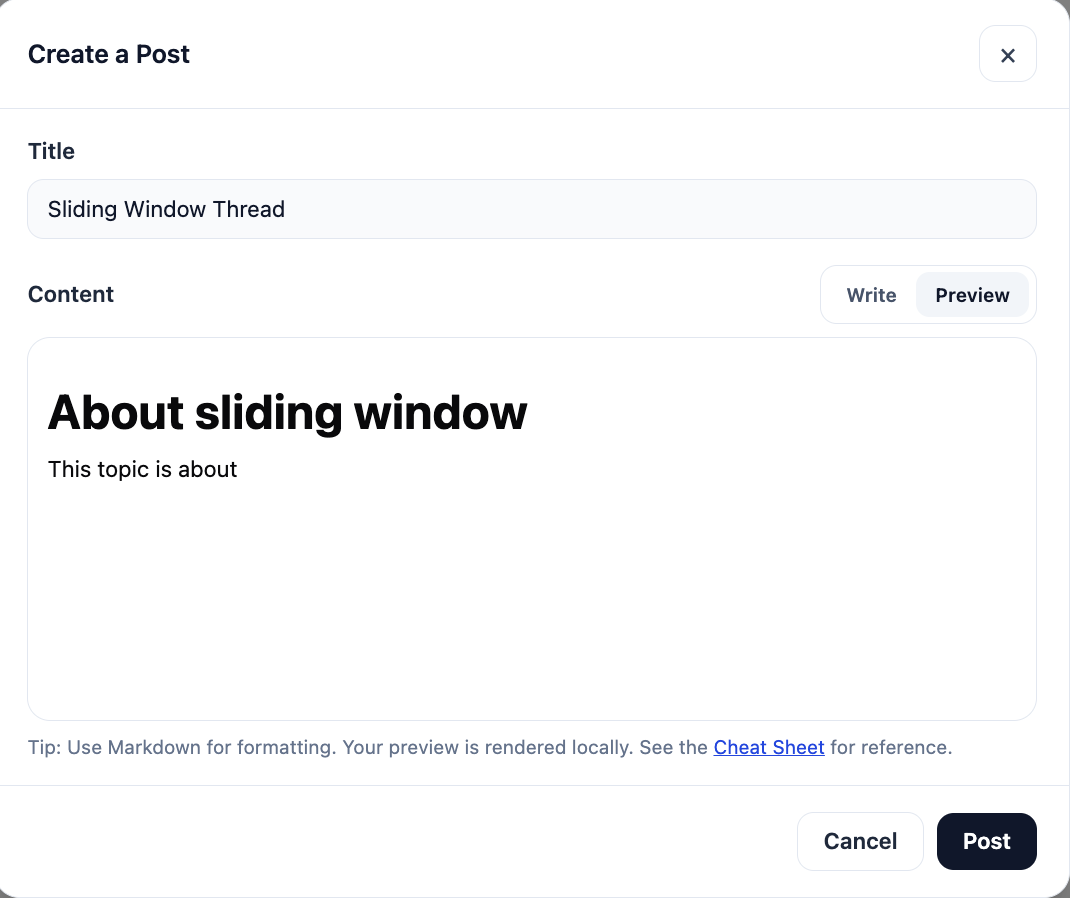
\includegraphics[width=1\textwidth]{Contents/Chapter 4/Mockup Design/Primary User/discussion-2.png}
    \vspace{0.6cm}
    \caption{Create Discussion}
\end{figure}

\subsubsection*{Contest Participation}

Primary users can participate in coding contests hosted on the platform by navigating to the Contest List page from the main navigation menu. This page displays a list of upcoming and ongoing contests, along with relevant details such as contest name, start time, end time, and duration.
\begin{figure}[H]
    \centering
    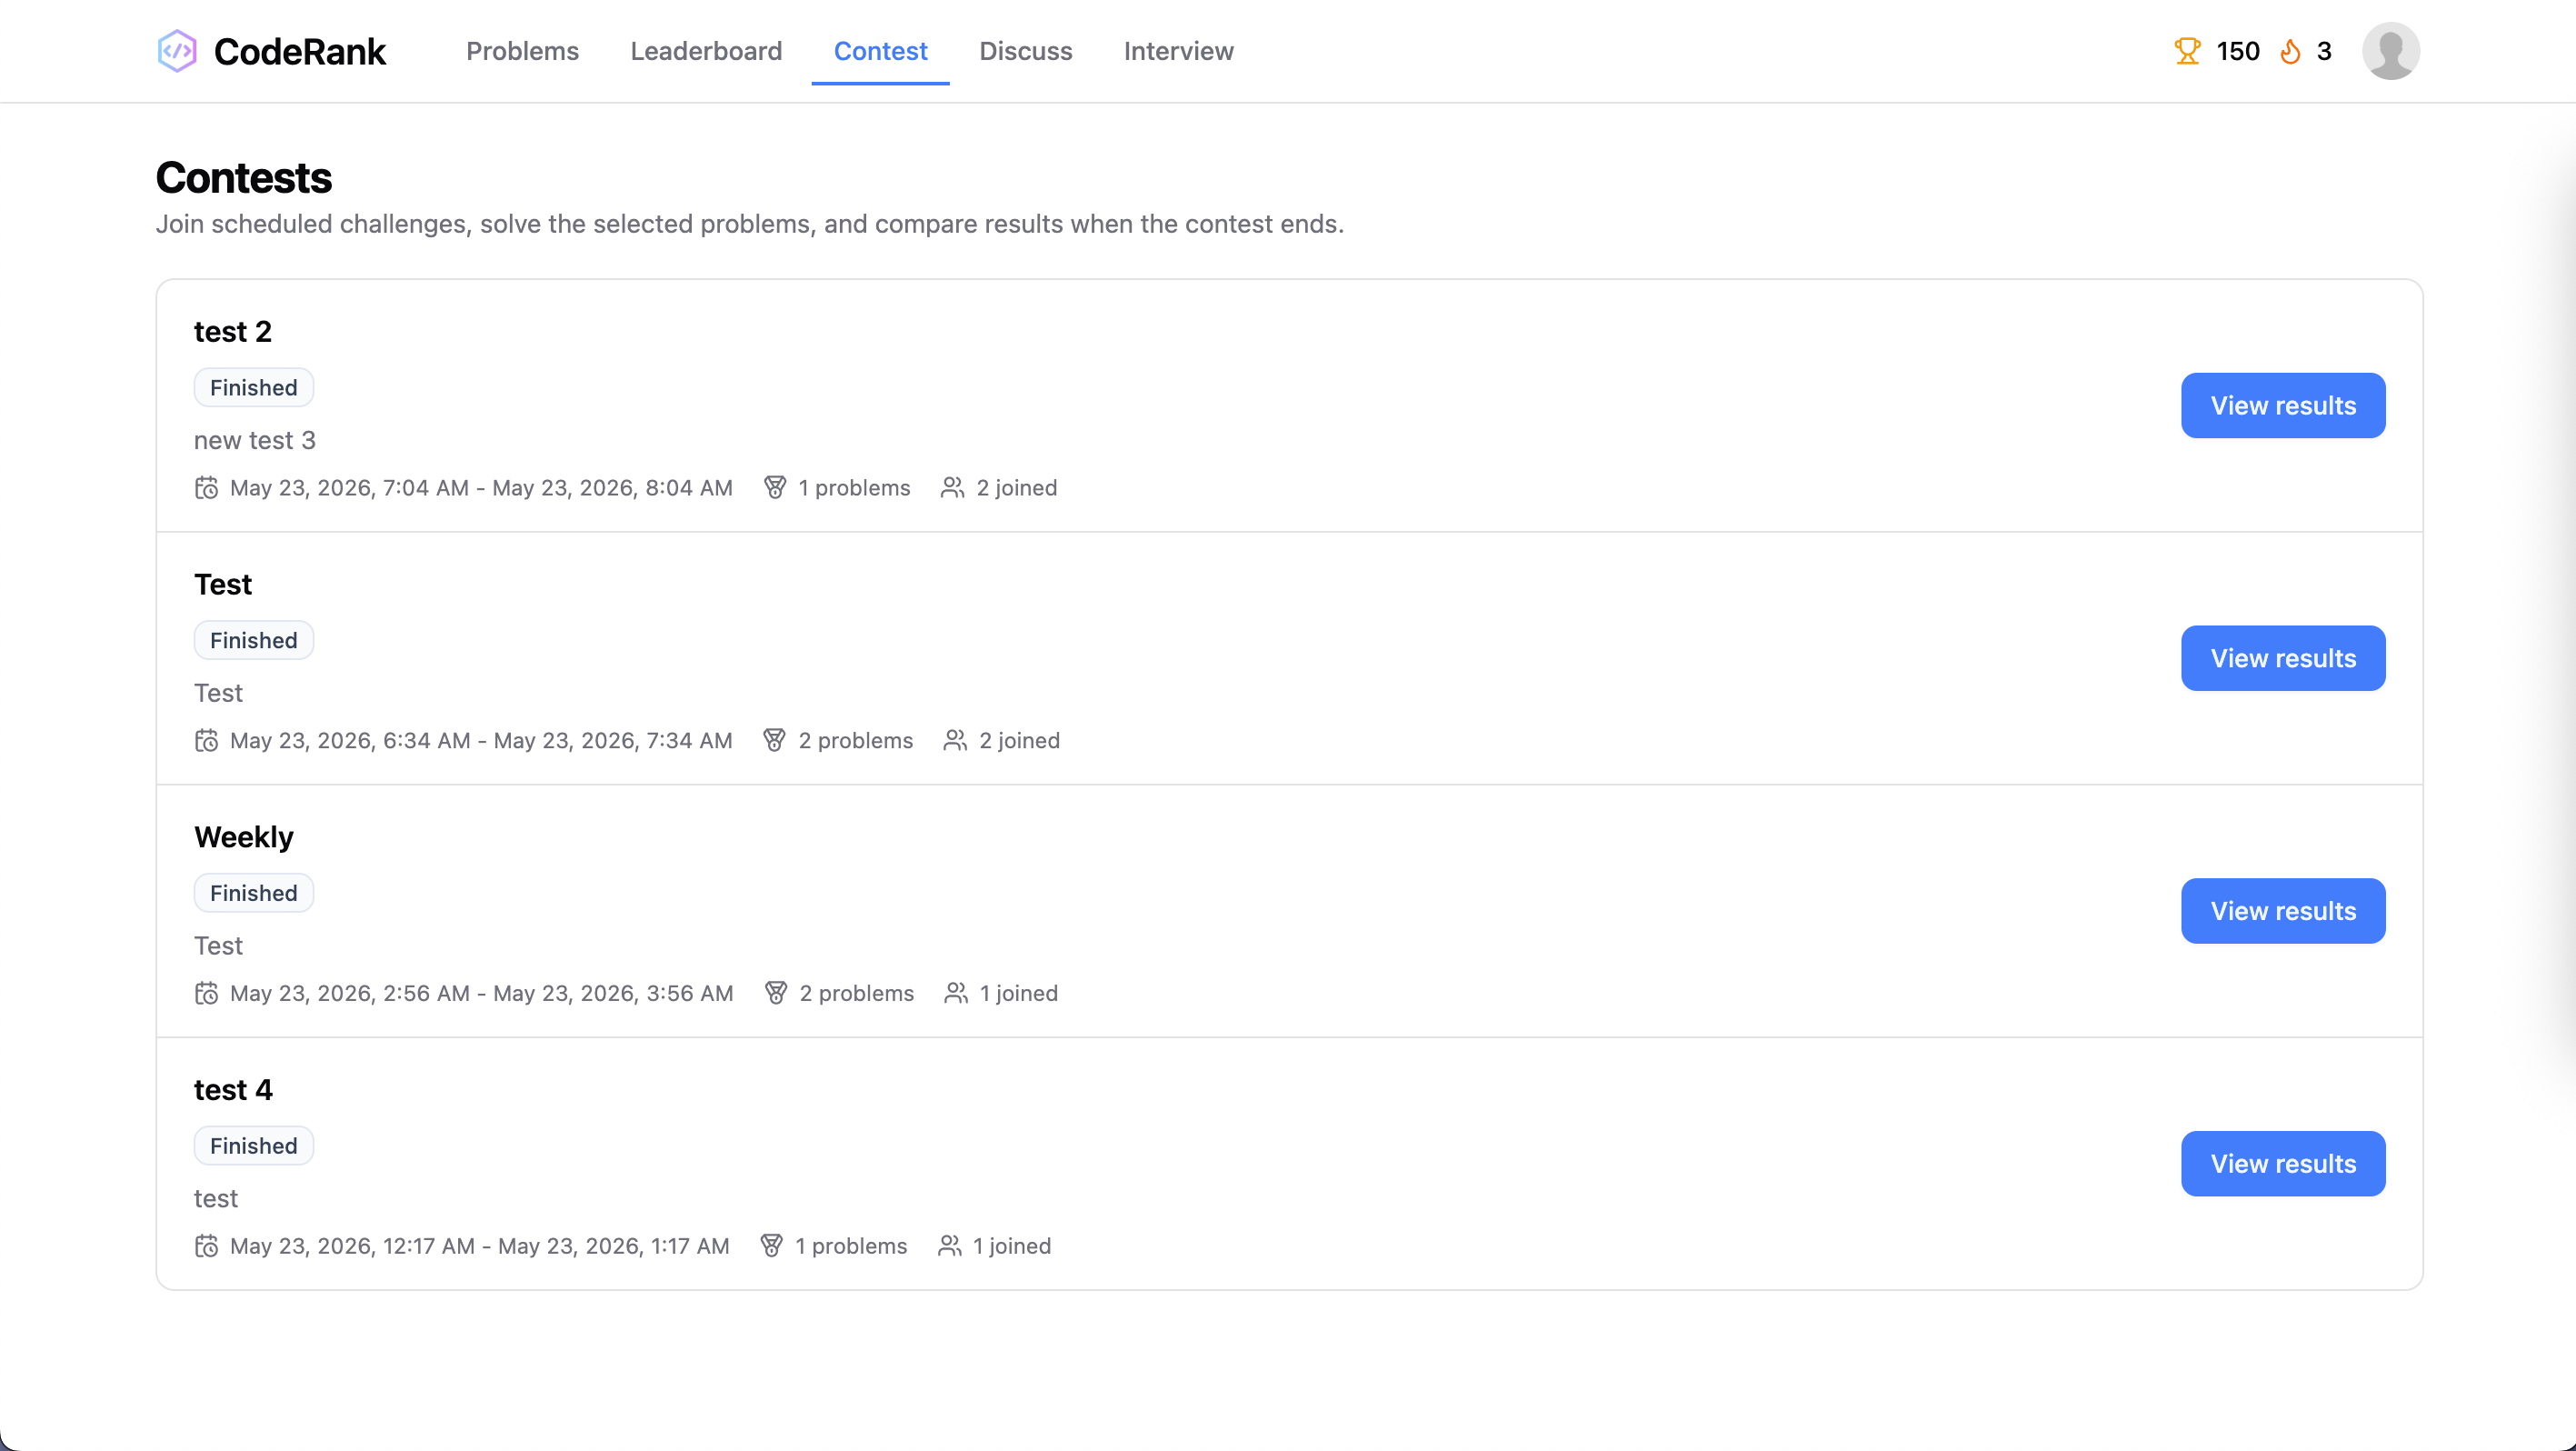
\includegraphics[width=1\textwidth]{Contents/Chapter 4/Mockup Design/Primary User/contest-1.png}
    \vspace{0.6cm}
    \caption{Contest List}
\end{figure}

In order to view the details of a specific contest, the user can click on the contest name in the Contest List. This will take them to the Contest Detail page, where they can see the information about the contest, including the list of problems included in the contest.
\begin{figure}[H]
    \centering
    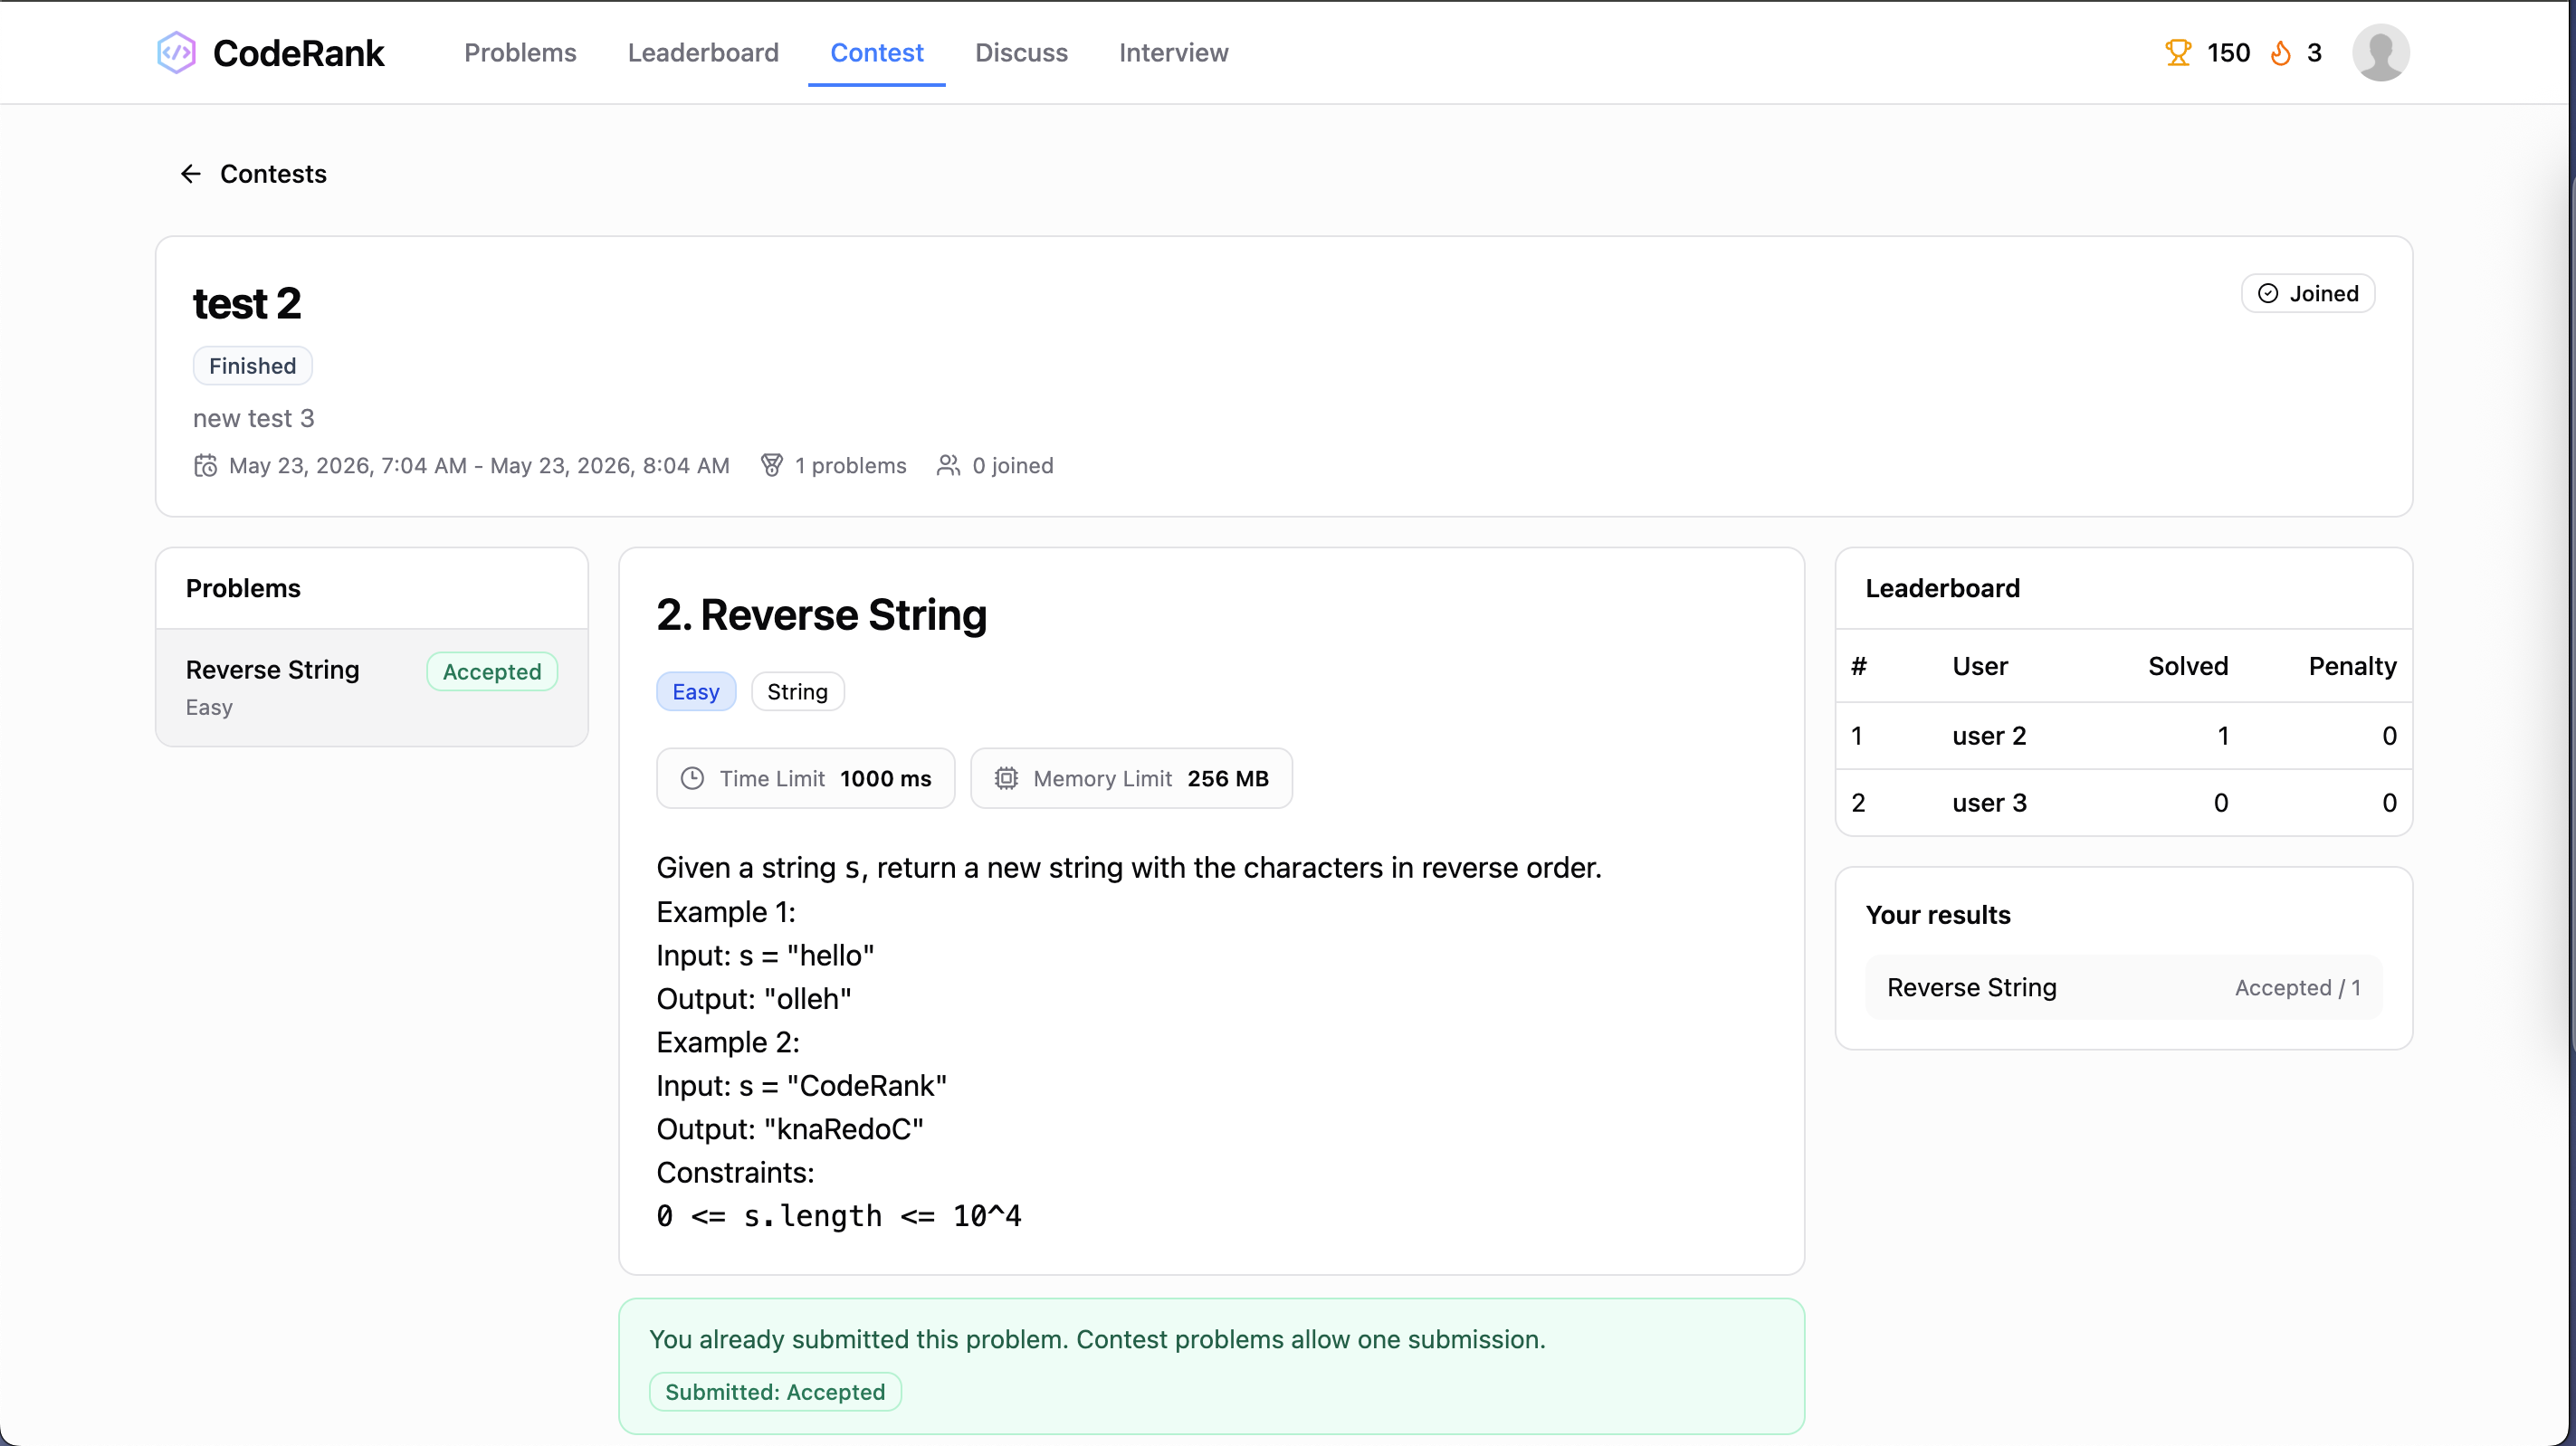
\includegraphics[width=1\textwidth]{Contents/Chapter 4/Mockup Design/Primary User/contest-2.png}
    \vspace{0.6cm}
    \caption{Contest Detail}
\end{figure}


In order to create a custom contest, moderator can go to the Contest monitor page. Here, they can enter the contest name, select problems to include in the contest, set the start and end time, and define other contest settings.
\begin{figure}[H]
    \centering
    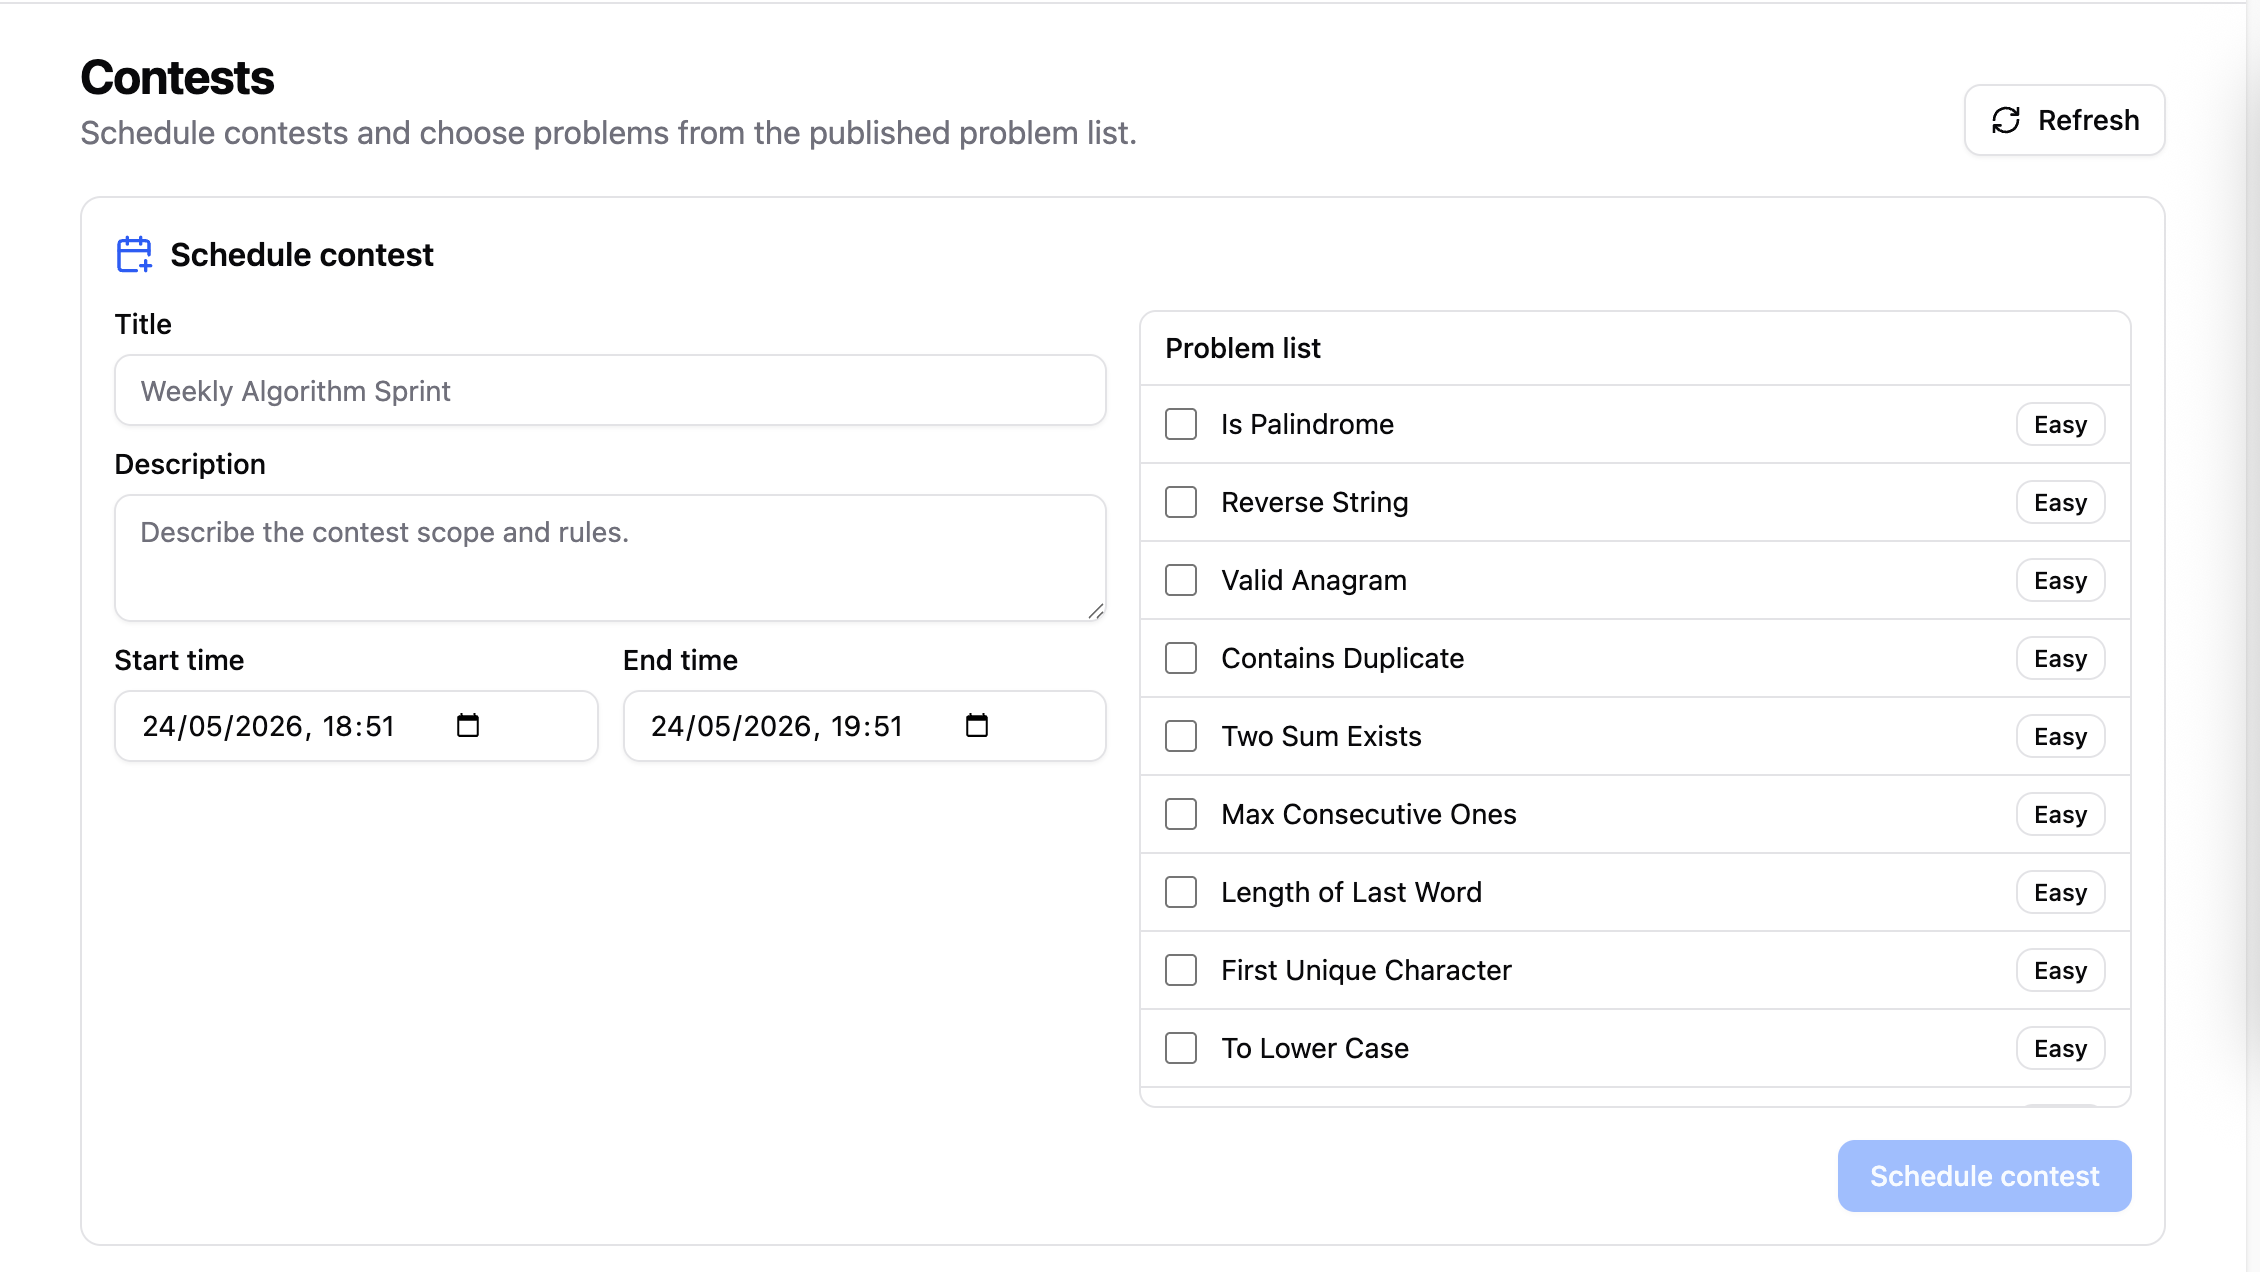
\includegraphics[width=1\textwidth]{Contents/Chapter 4/Mockup Design/Primary User/contest-3.png}
    \vspace{0.6cm}
    \caption{Contest Creation}
\end{figure}

\subsubsection*{Interview Preparation}
Primary users can access the Interview Preparation feature from the main navigation menu. The Interview Preparation feature provides users with a curated list of coding problems and resources specifically designed to help them prepare for technical interviews. In the Interview Preparation page, there will be a conversation history section on the left side, displaying a list of previous interview preparation sessions. Users can select a session to view the details and continue their preparation or create a new session by clicking the \textbf{New Conversation} button.
\begin{figure}[H]
    \centering
    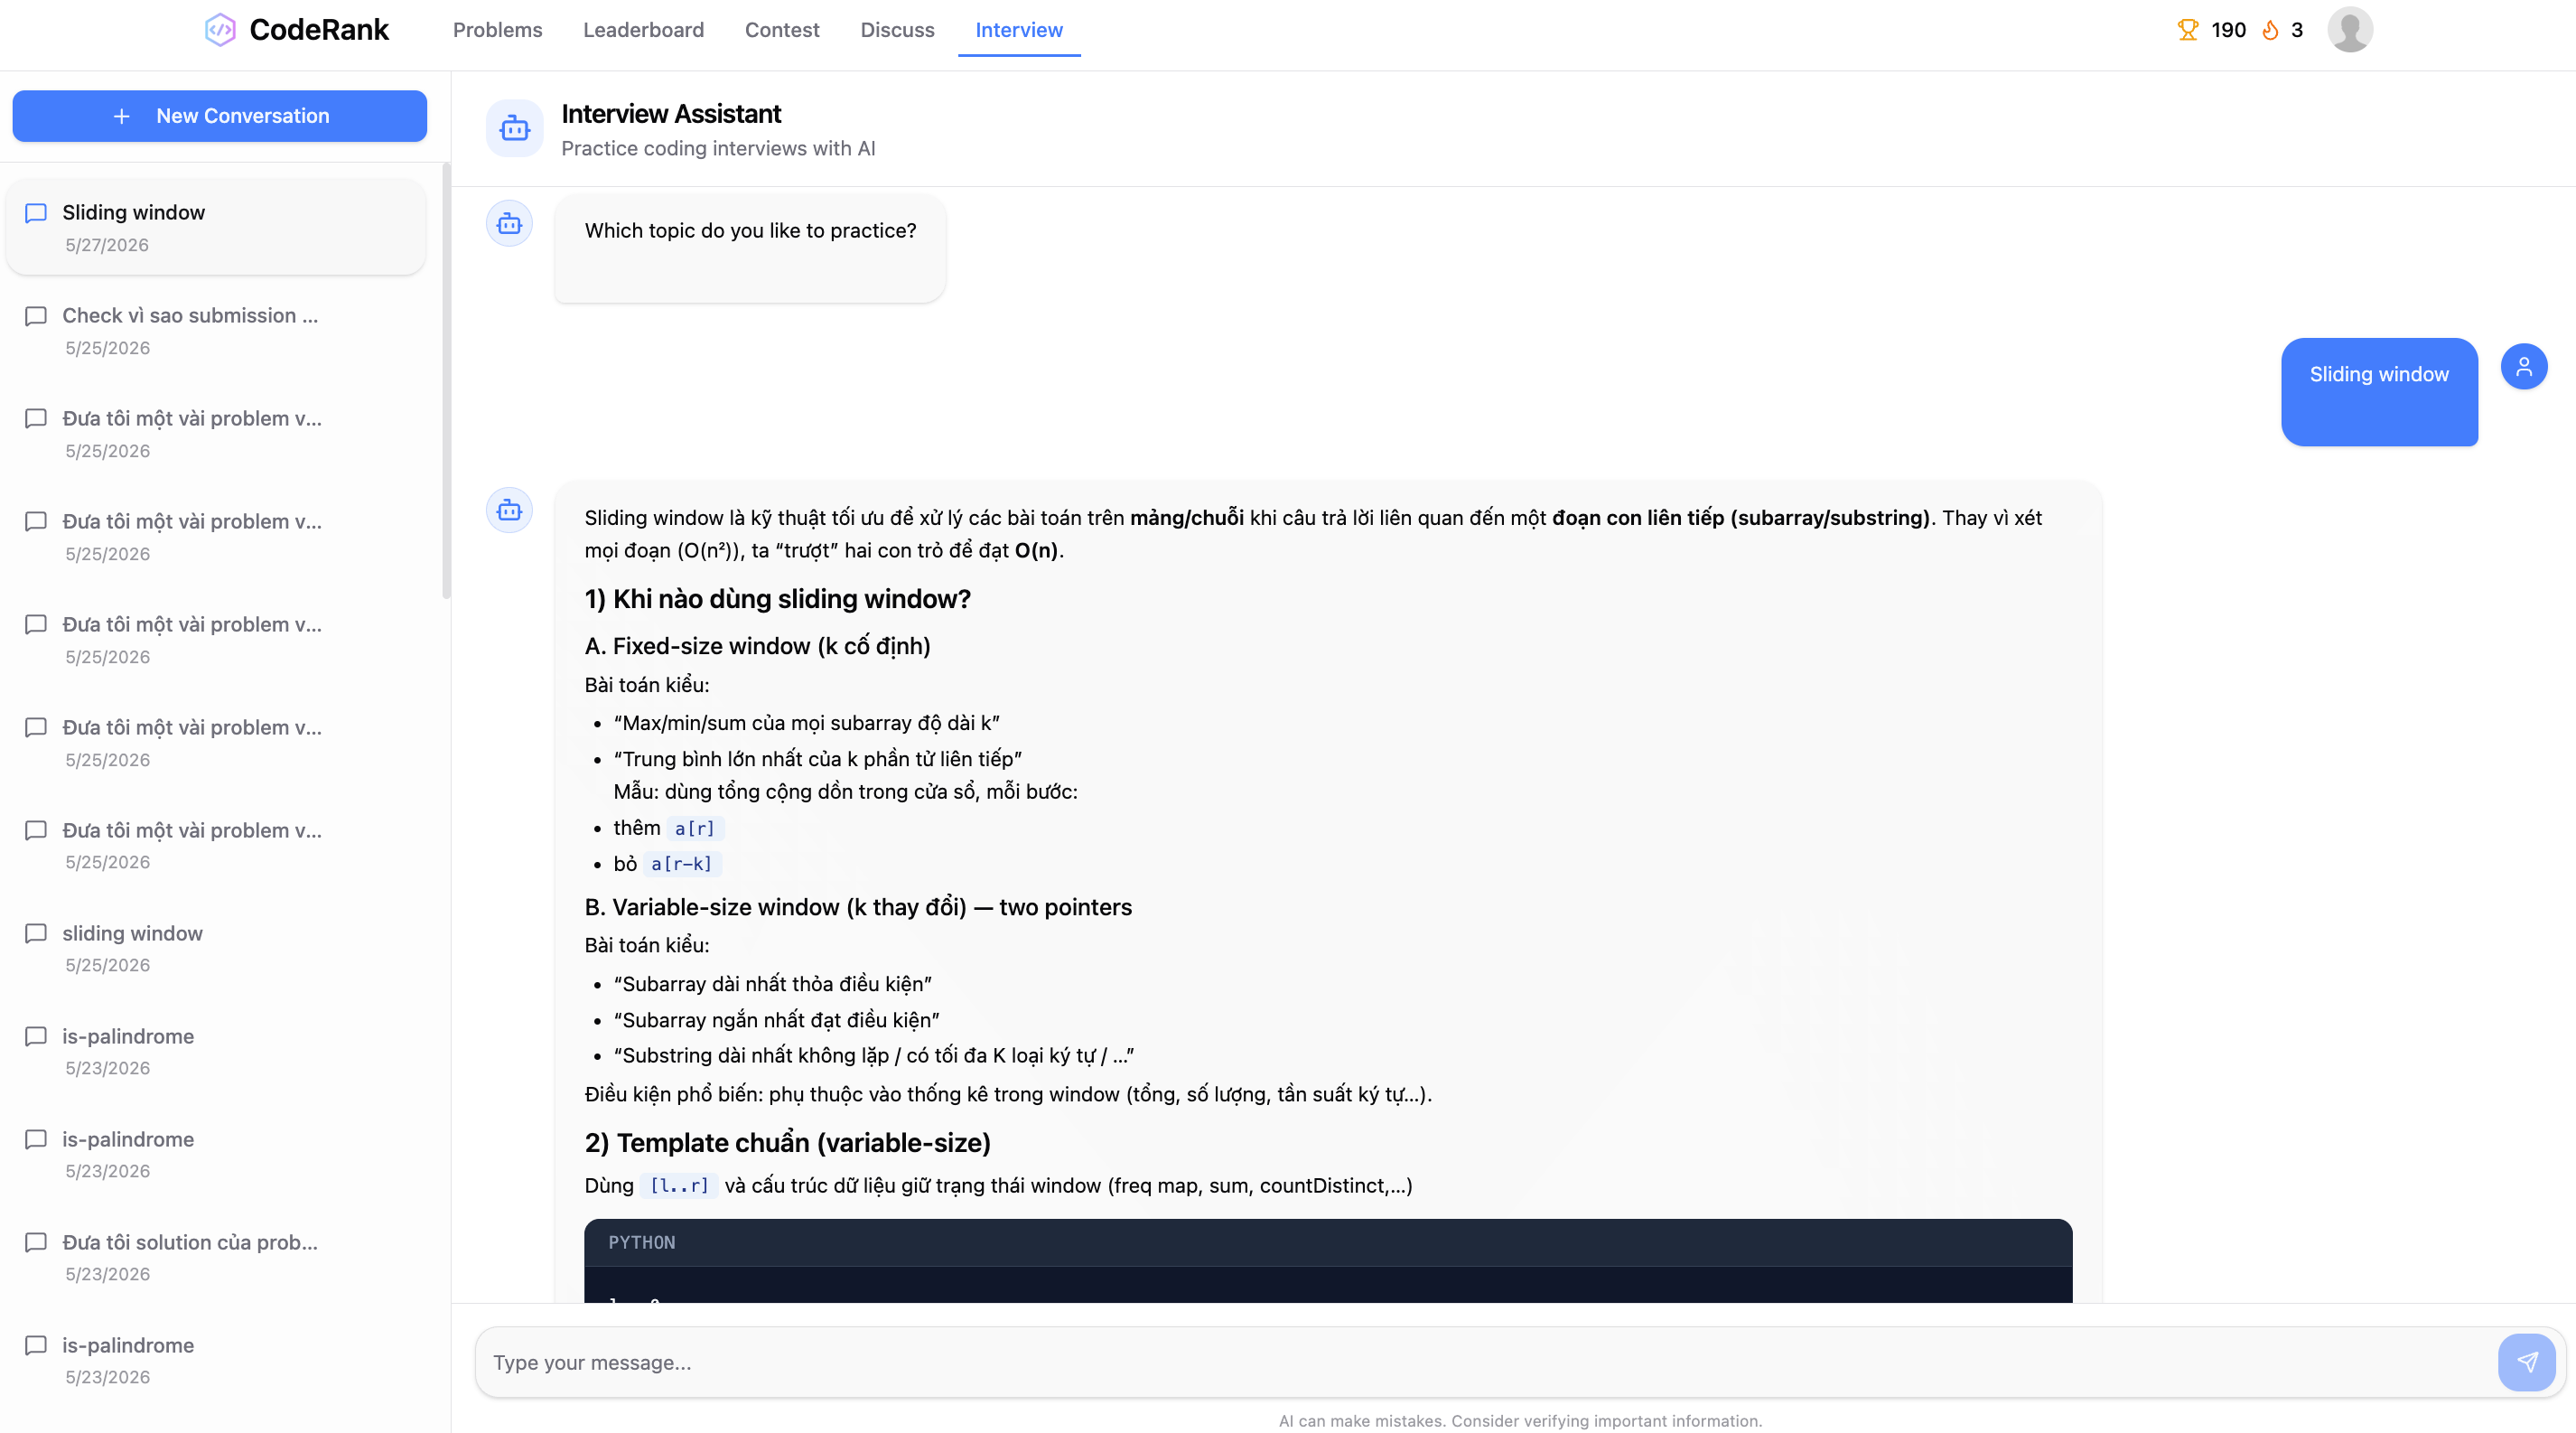
\includegraphics[width=1\textwidth]{Contents/Chapter 4/Mockup Design/Primary User/interview-1.png}
    \vspace{0.6cm}
    \caption{Interview Preparation Page}
\end{figure}

\subsection{Moderator/Admin flow}

After logging in as a Moderator/Admin, the user will be directed to the Moderator/Superadmin Dashboard. This dashboard provides an overview of key metrics and functionalities available to moderators and administrators, allowing them to manage the platform effectively.
\begin{figure}[H]
    \centering
    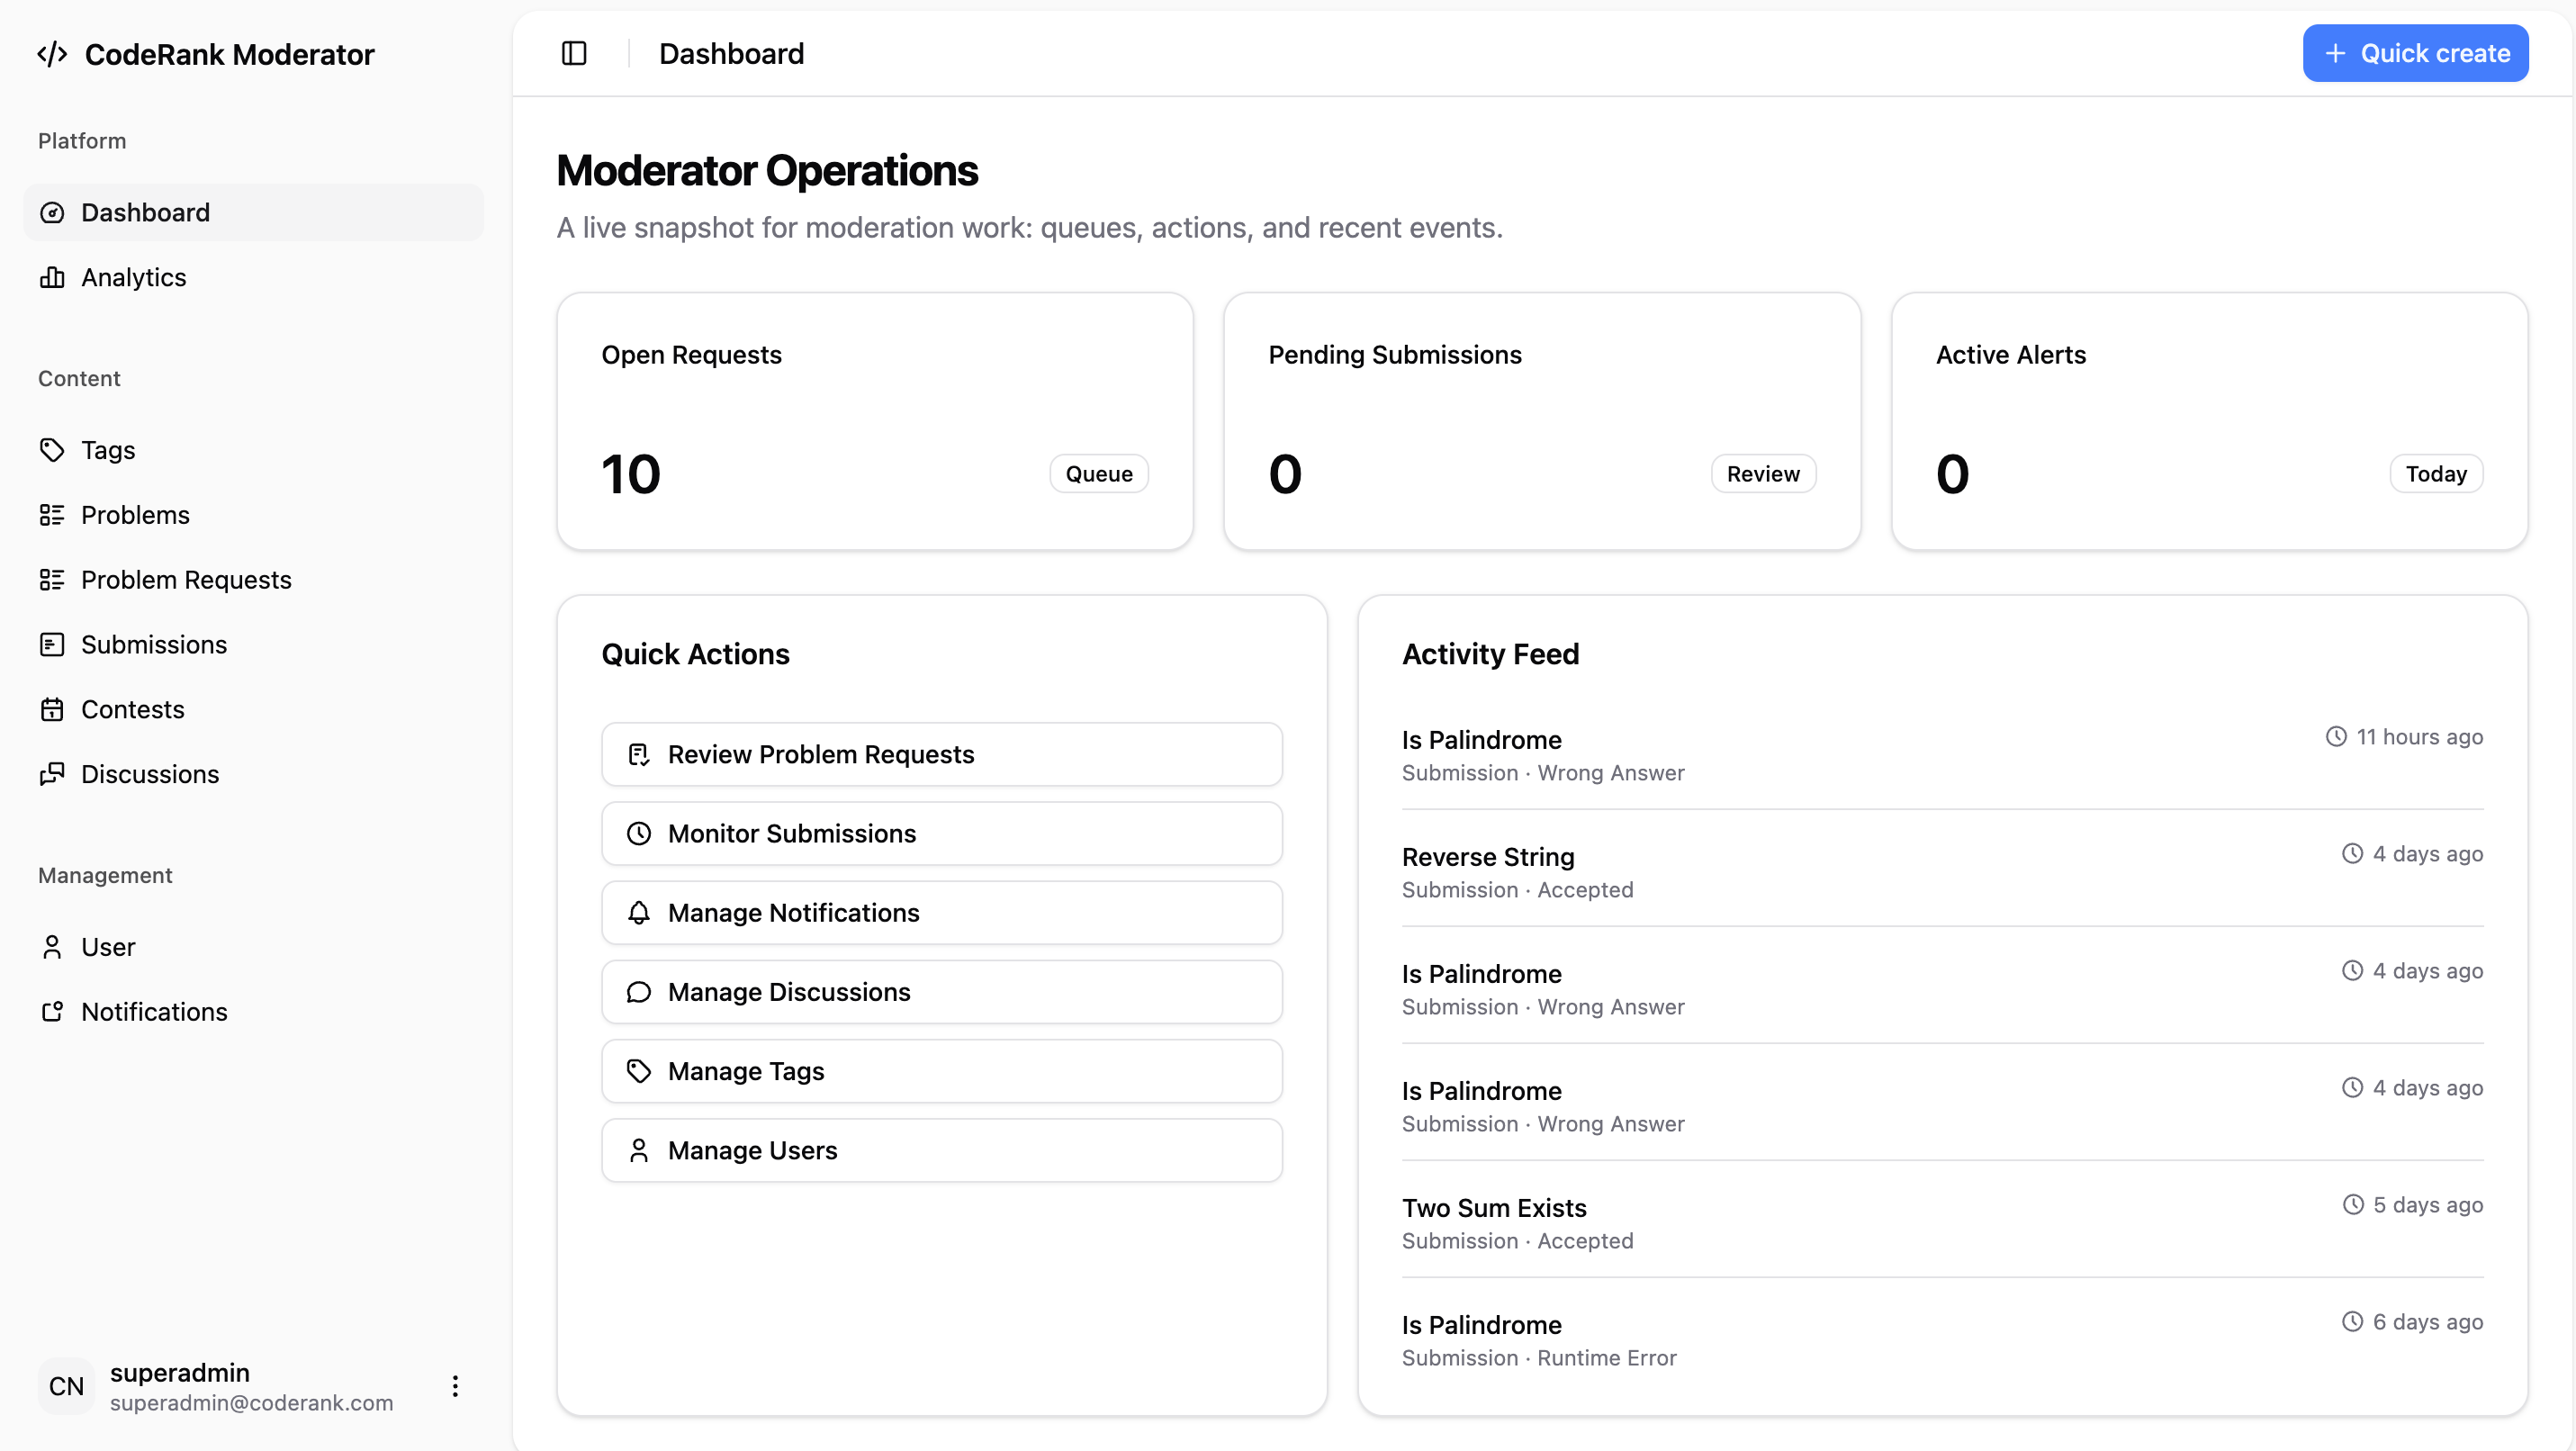
\includegraphics[width=1\textwidth]{Contents/Chapter 4/Mockup Design/Admin/admin-1.png}
    \vspace{0.6cm}
    \caption{Moderator Dashboard}
\end{figure}

The Moderator/Admin dashboard also provides centralized management interfaces for major platform resources. These interfaces allow privileged users to inspect system data, update operational content, and perform moderation actions from a consistent administrative workspace.

The Discussion Management interface displays all discussion threads available in the system. From this screen, Moderators/Admins can open a discussion detail page, review its comments, edit inappropriate content when necessary, or delete discussions and comments that violate platform policies.
\begin{figure}[H]
    \centering
    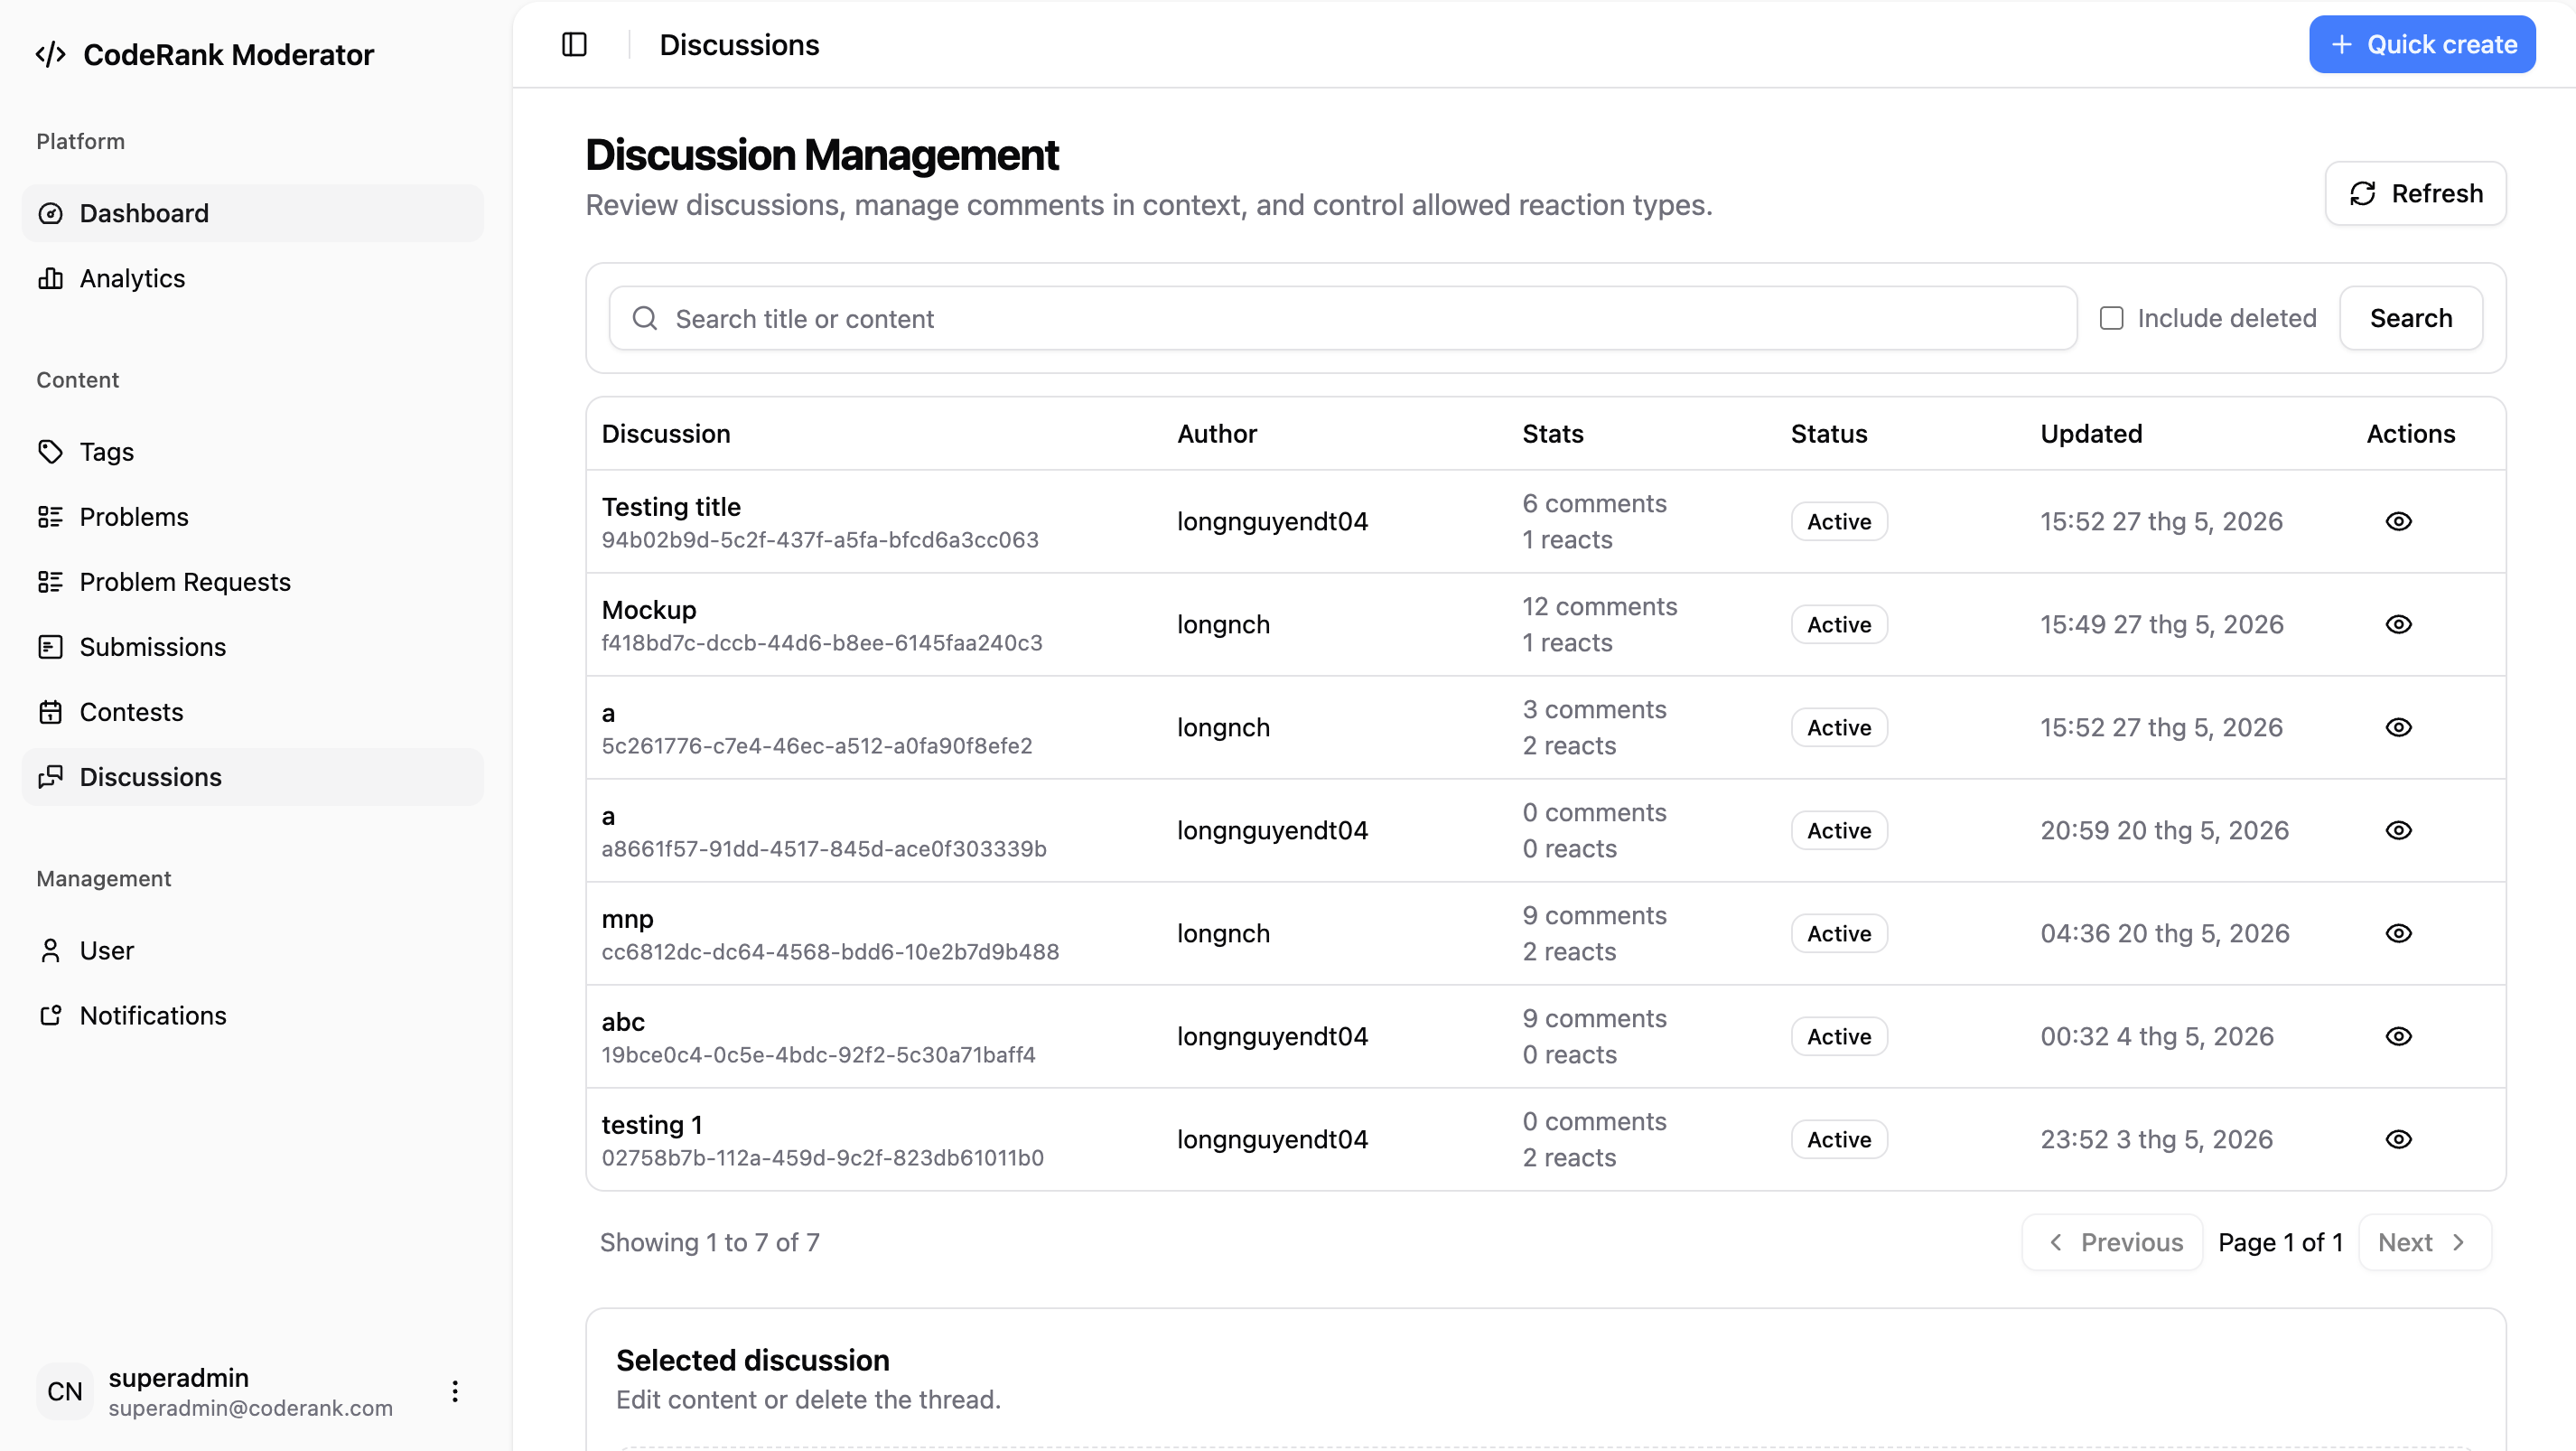
\includegraphics[width=1\textwidth]{Contents/Chapter 4/Mockup Design/Admin/discussion_management.png}
    \vspace{0.6cm}
    \caption{Discussion Management}
\end{figure}

The Contest Management interface supports the creation, editing, and maintenance of contest content. Moderators/Admins can configure contest information, update contest details, and manage contest-related content from a single administrative view.
\begin{figure}[H]
    \centering
    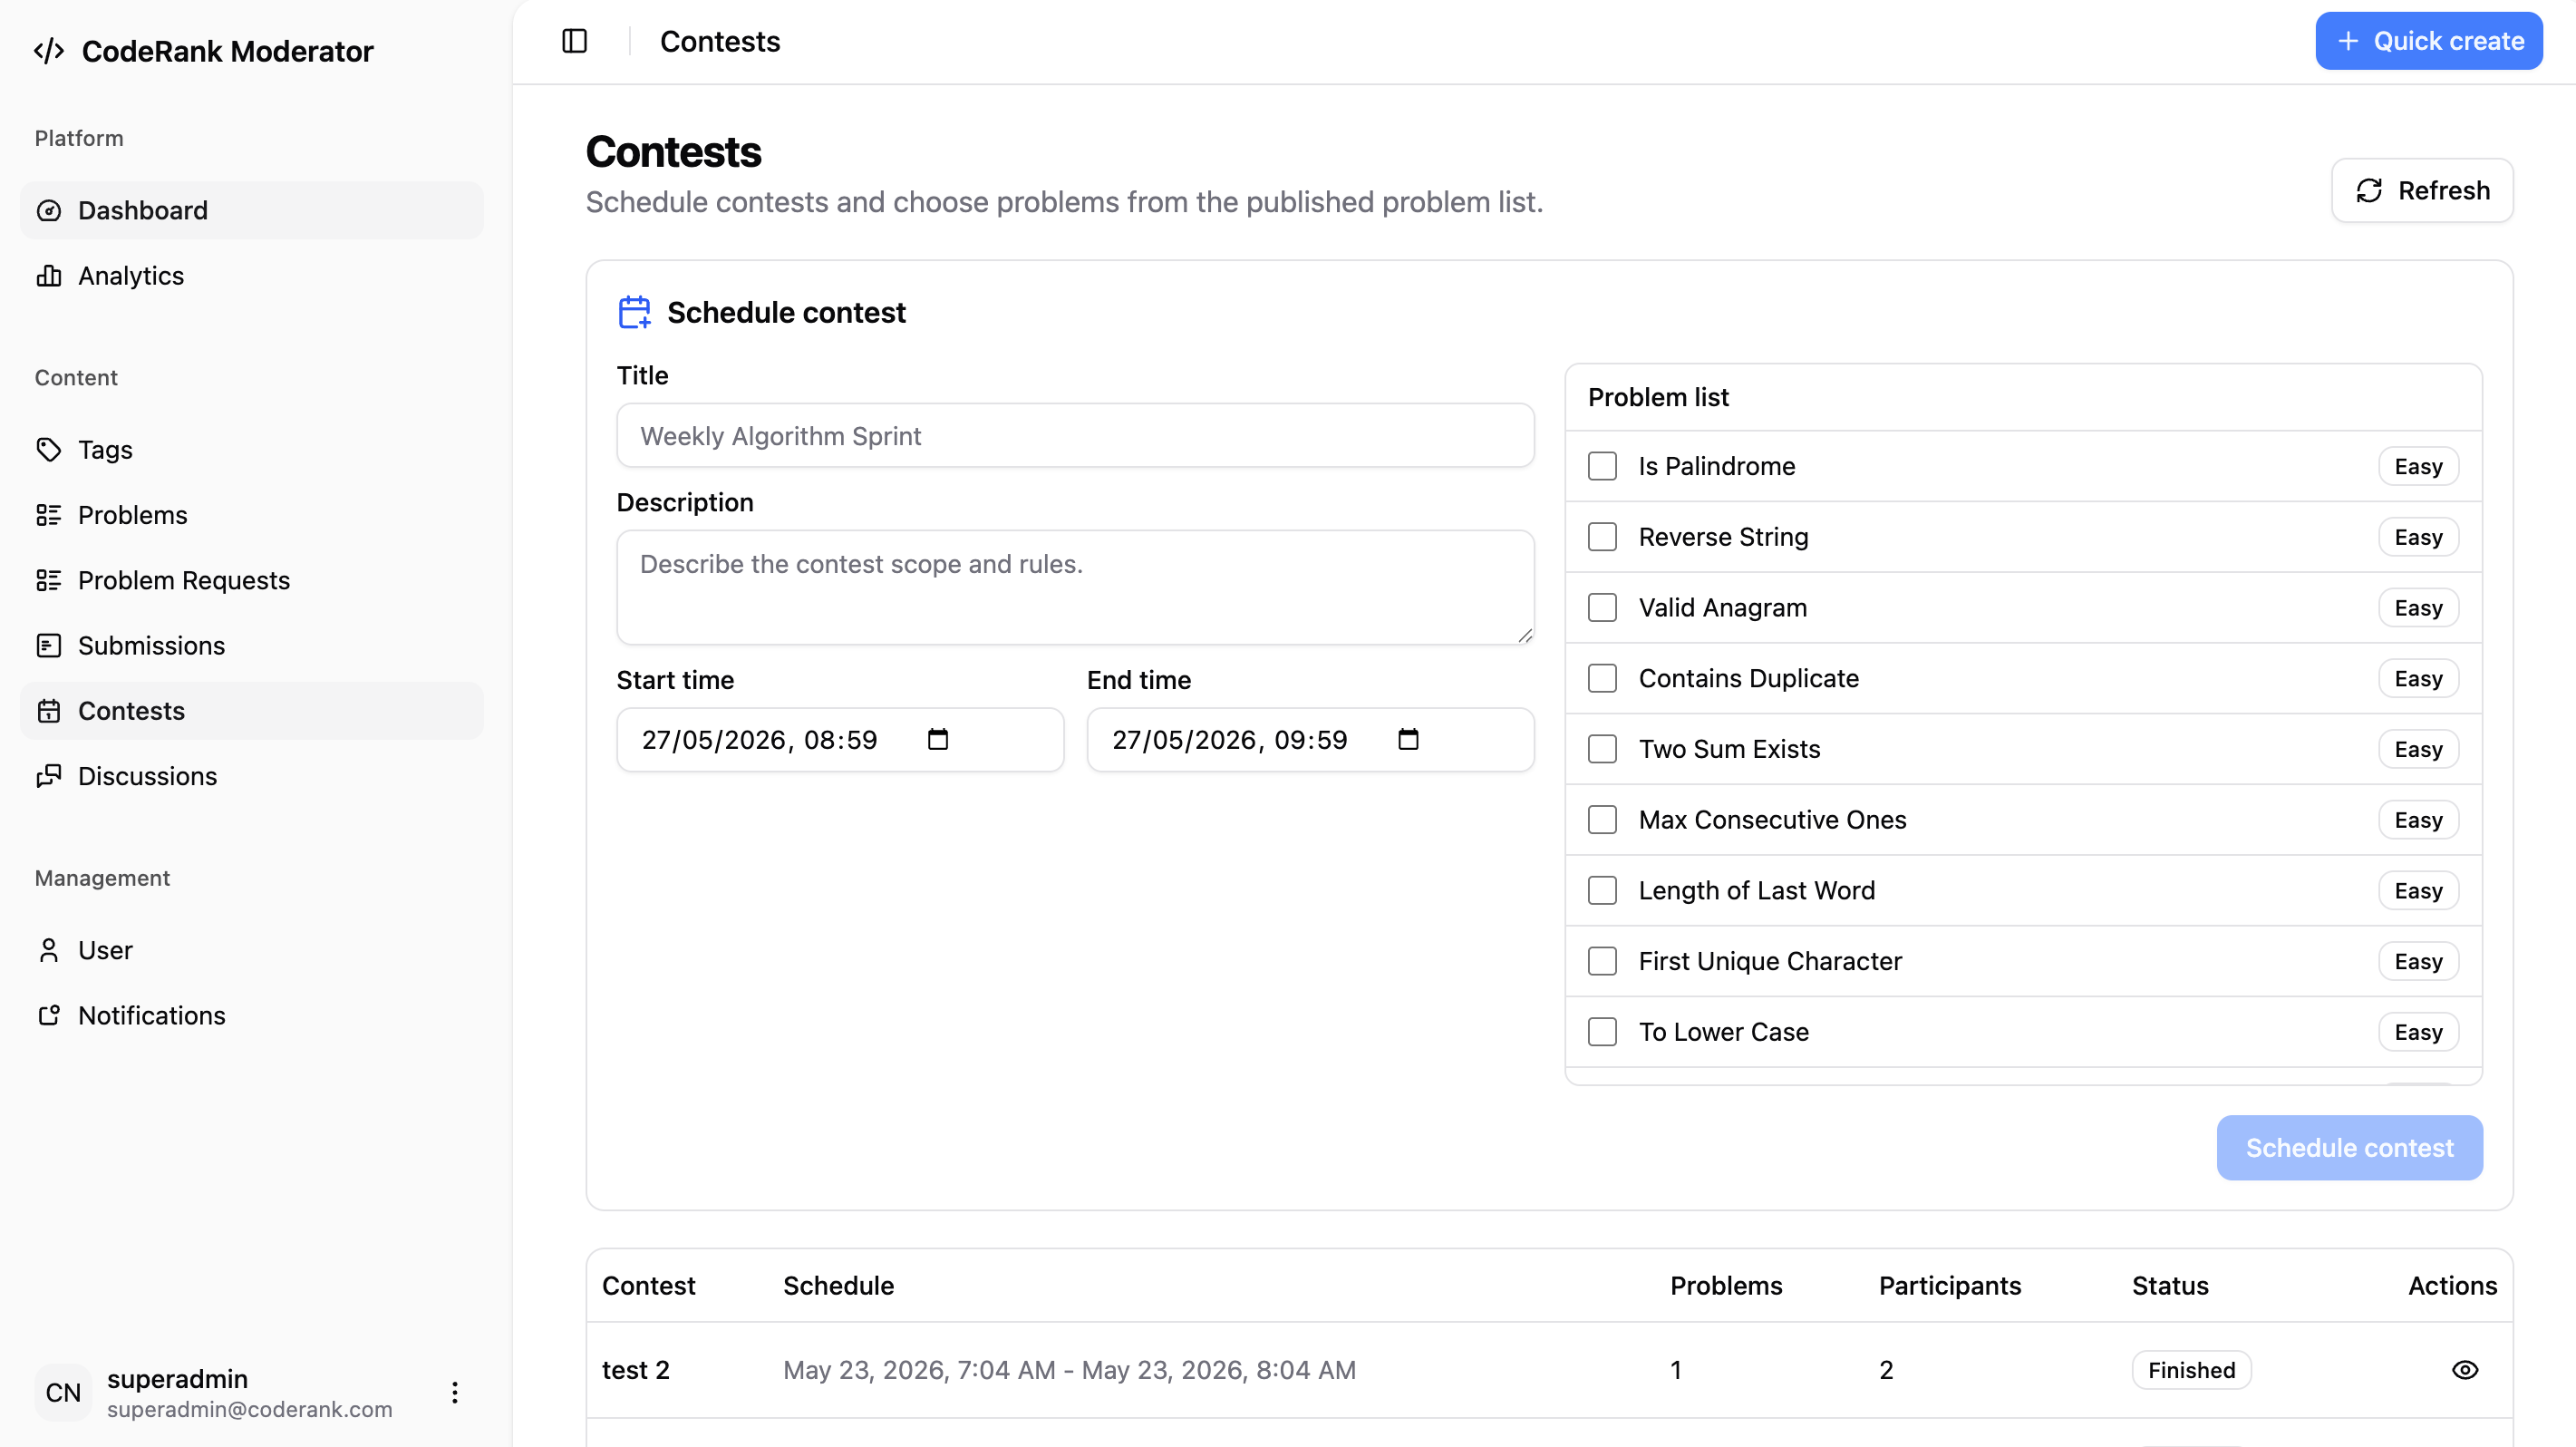
\includegraphics[width=1\textwidth]{Contents/Chapter 4/Mockup Design/Admin/contest_management.png}
    \vspace{0.6cm}
    \caption{Contest Management}
\end{figure}

The User Management interface is used to administer user accounts across the platform. It allows Moderators/Admins to view user details, delete users when required, and toggle account status to enable or disable access according to moderation decisions.
\begin{figure}[H]
    \centering
    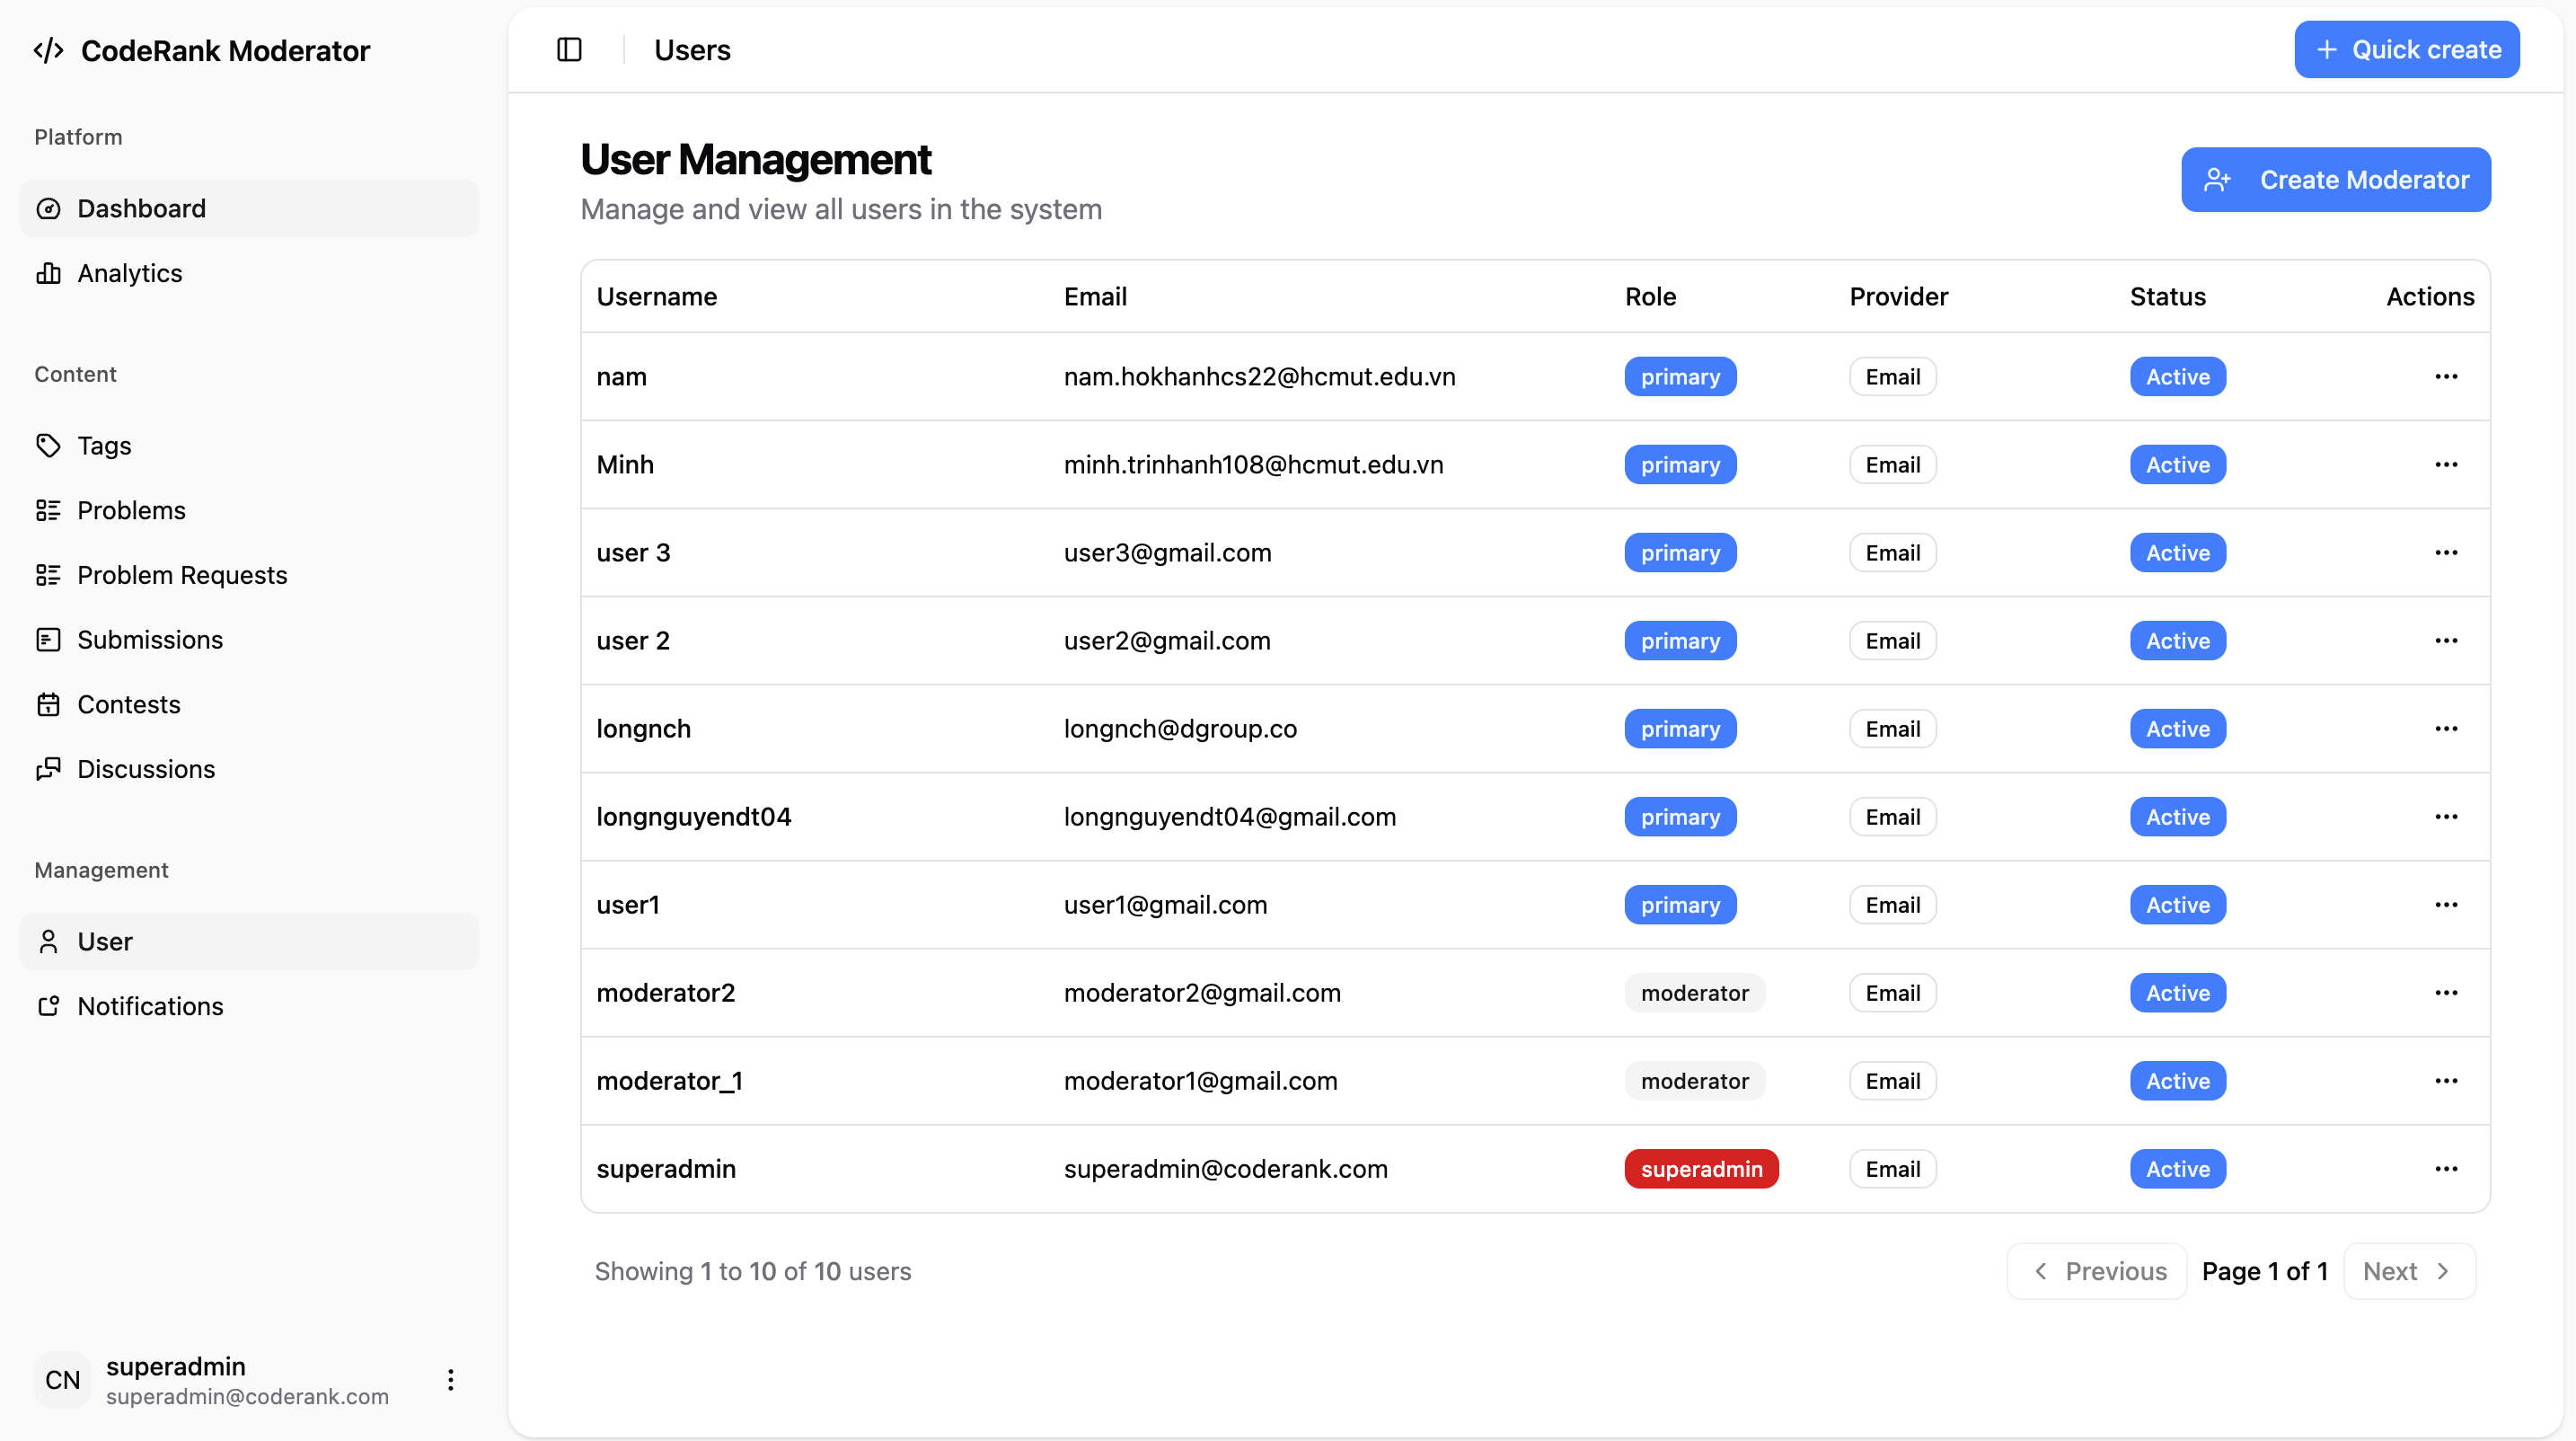
\includegraphics[width=1\textwidth]{Contents/Chapter 4/Mockup Design/Admin/user_management.png}
    \vspace{0.6cm}
    \caption{User Management}
\end{figure}

The Submission Management interface provides visibility into user submissions in the system. It helps Moderators/Admins review submission records, monitor judging results, and inspect submission-related information for operational or moderation purposes.
\begin{figure}[H]
    \centering
    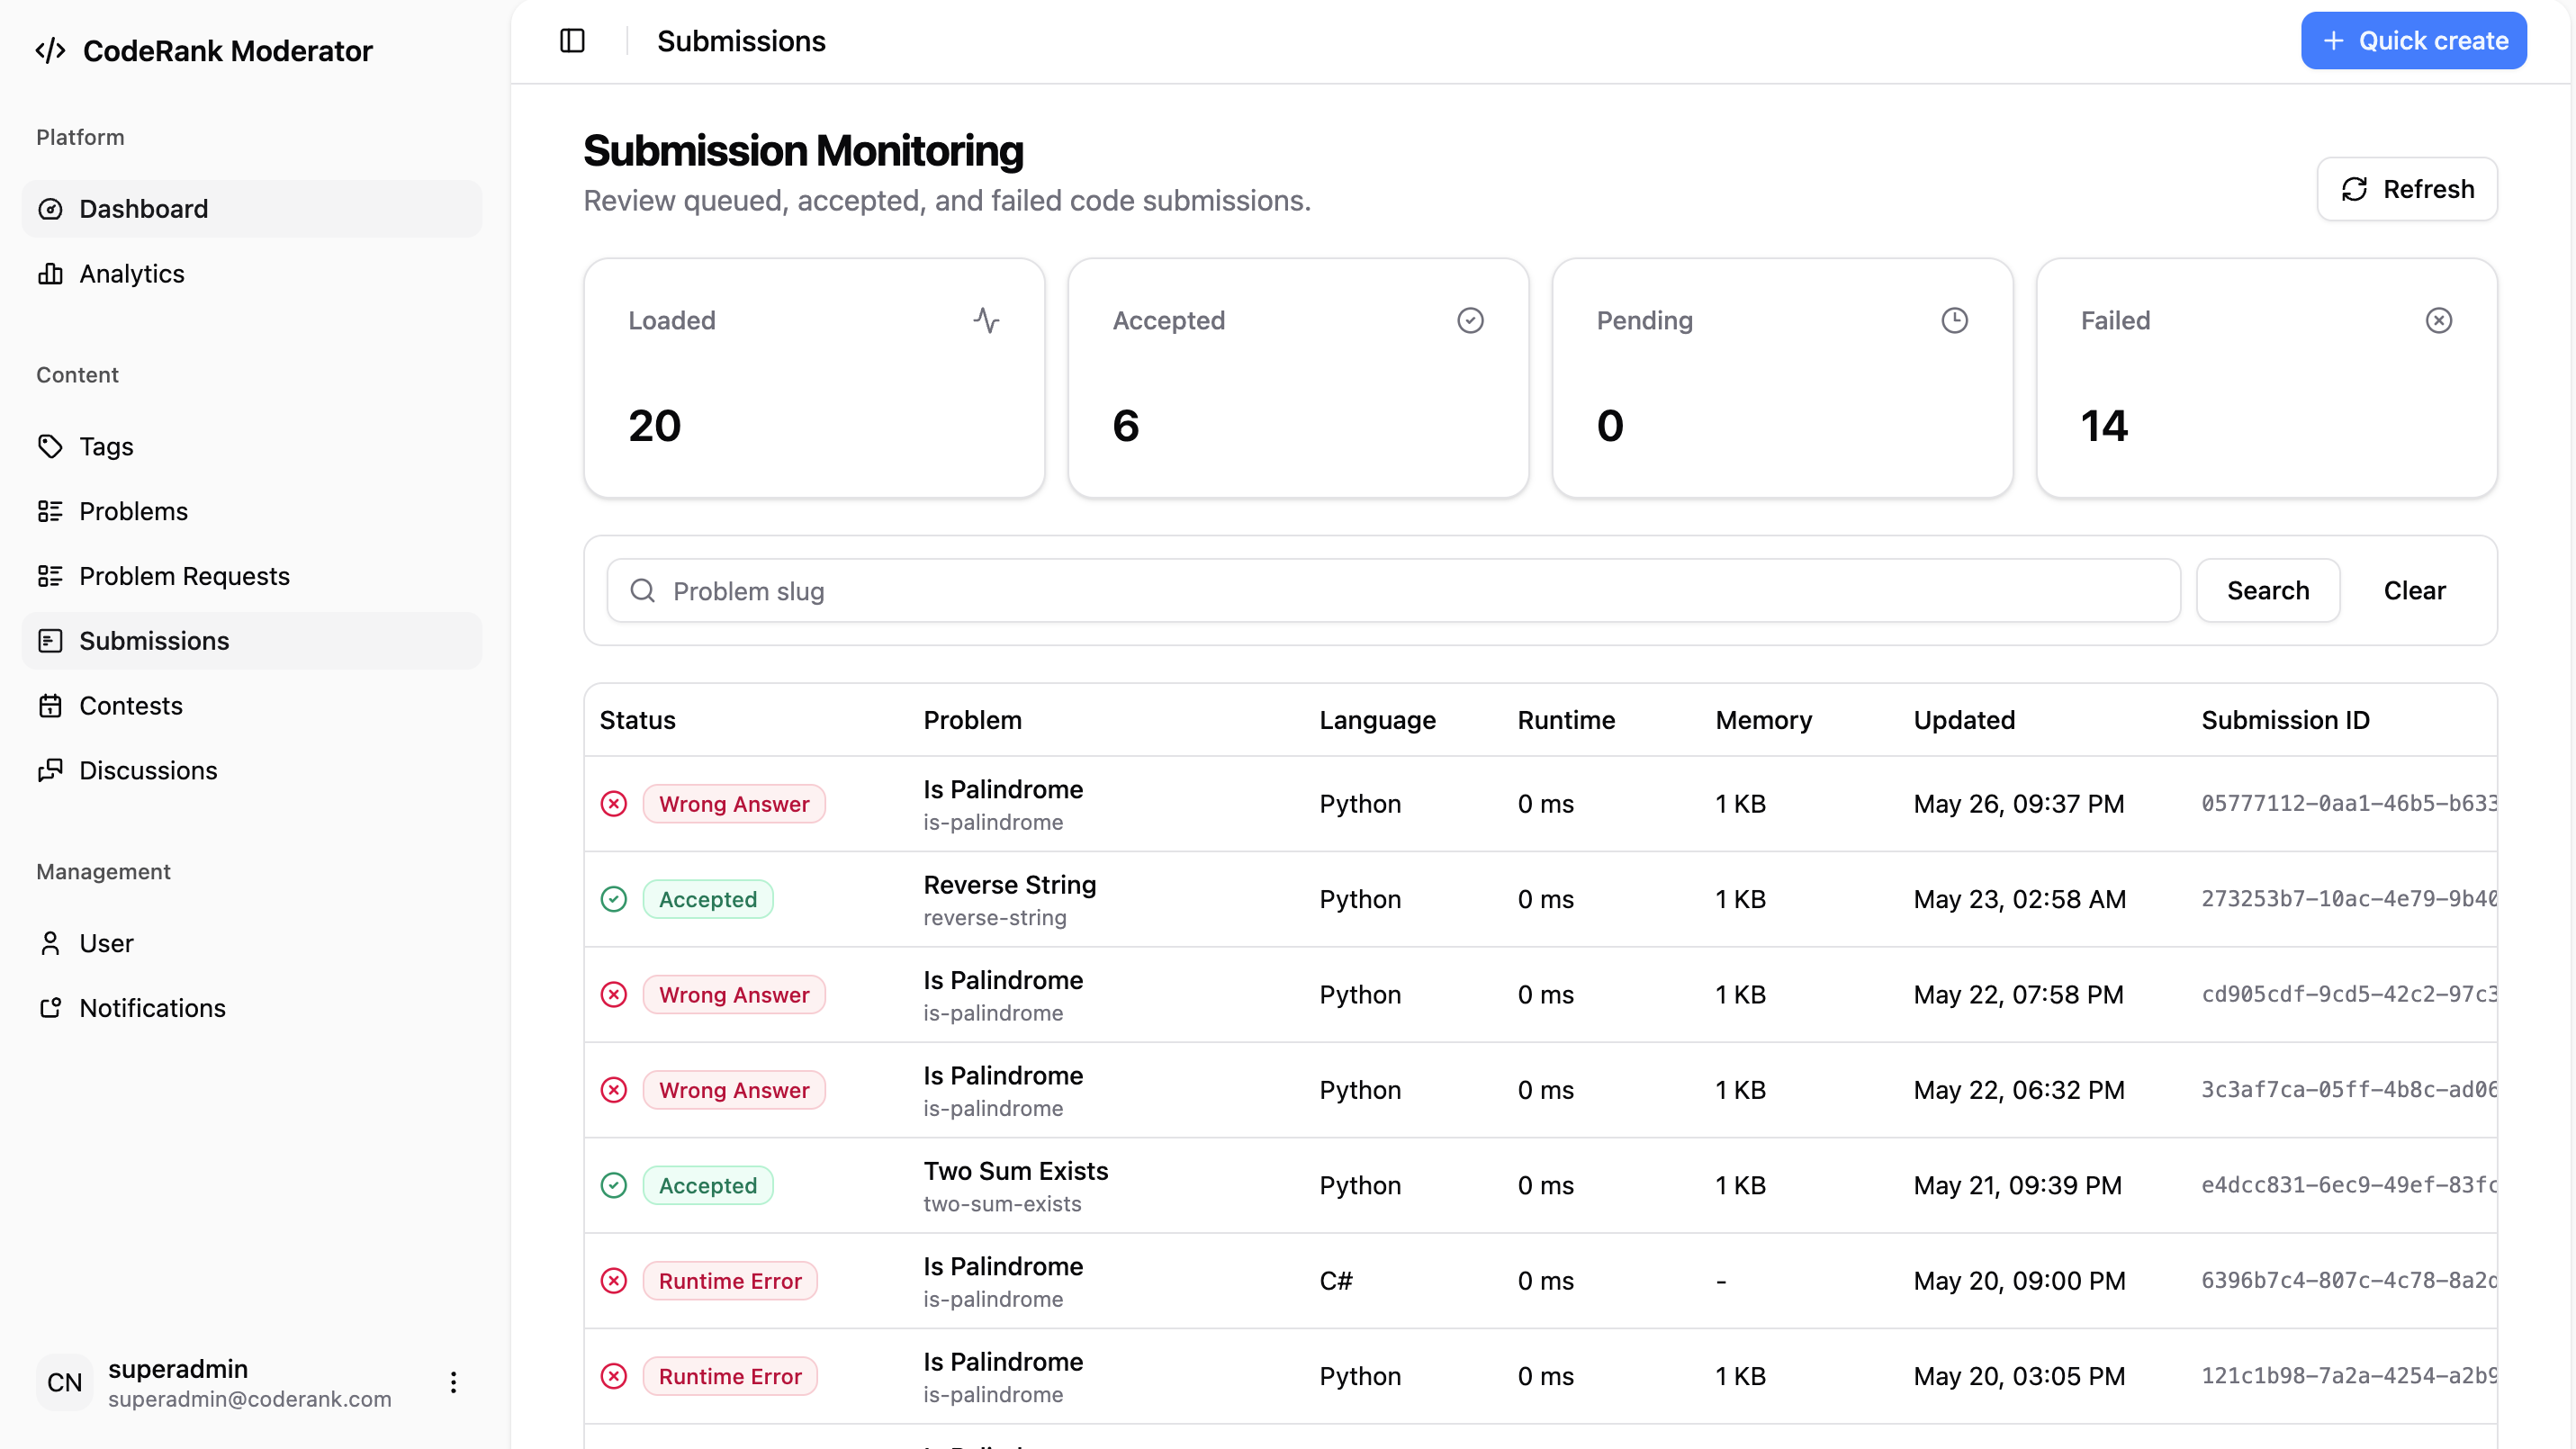
\includegraphics[width=1\textwidth]{Contents/Chapter 4/Mockup Design/Admin/submission_management.png}
    \vspace{0.6cm}
    \caption{Submission Management}
\end{figure}

The Notification Management interface is used to manage global notifications displayed on user-facing pages. Moderators/Admins can create new notifications, view existing notification details, delete outdated notifications, and control whether a notification is visible to users.
\begin{figure}[H]
    \centering
    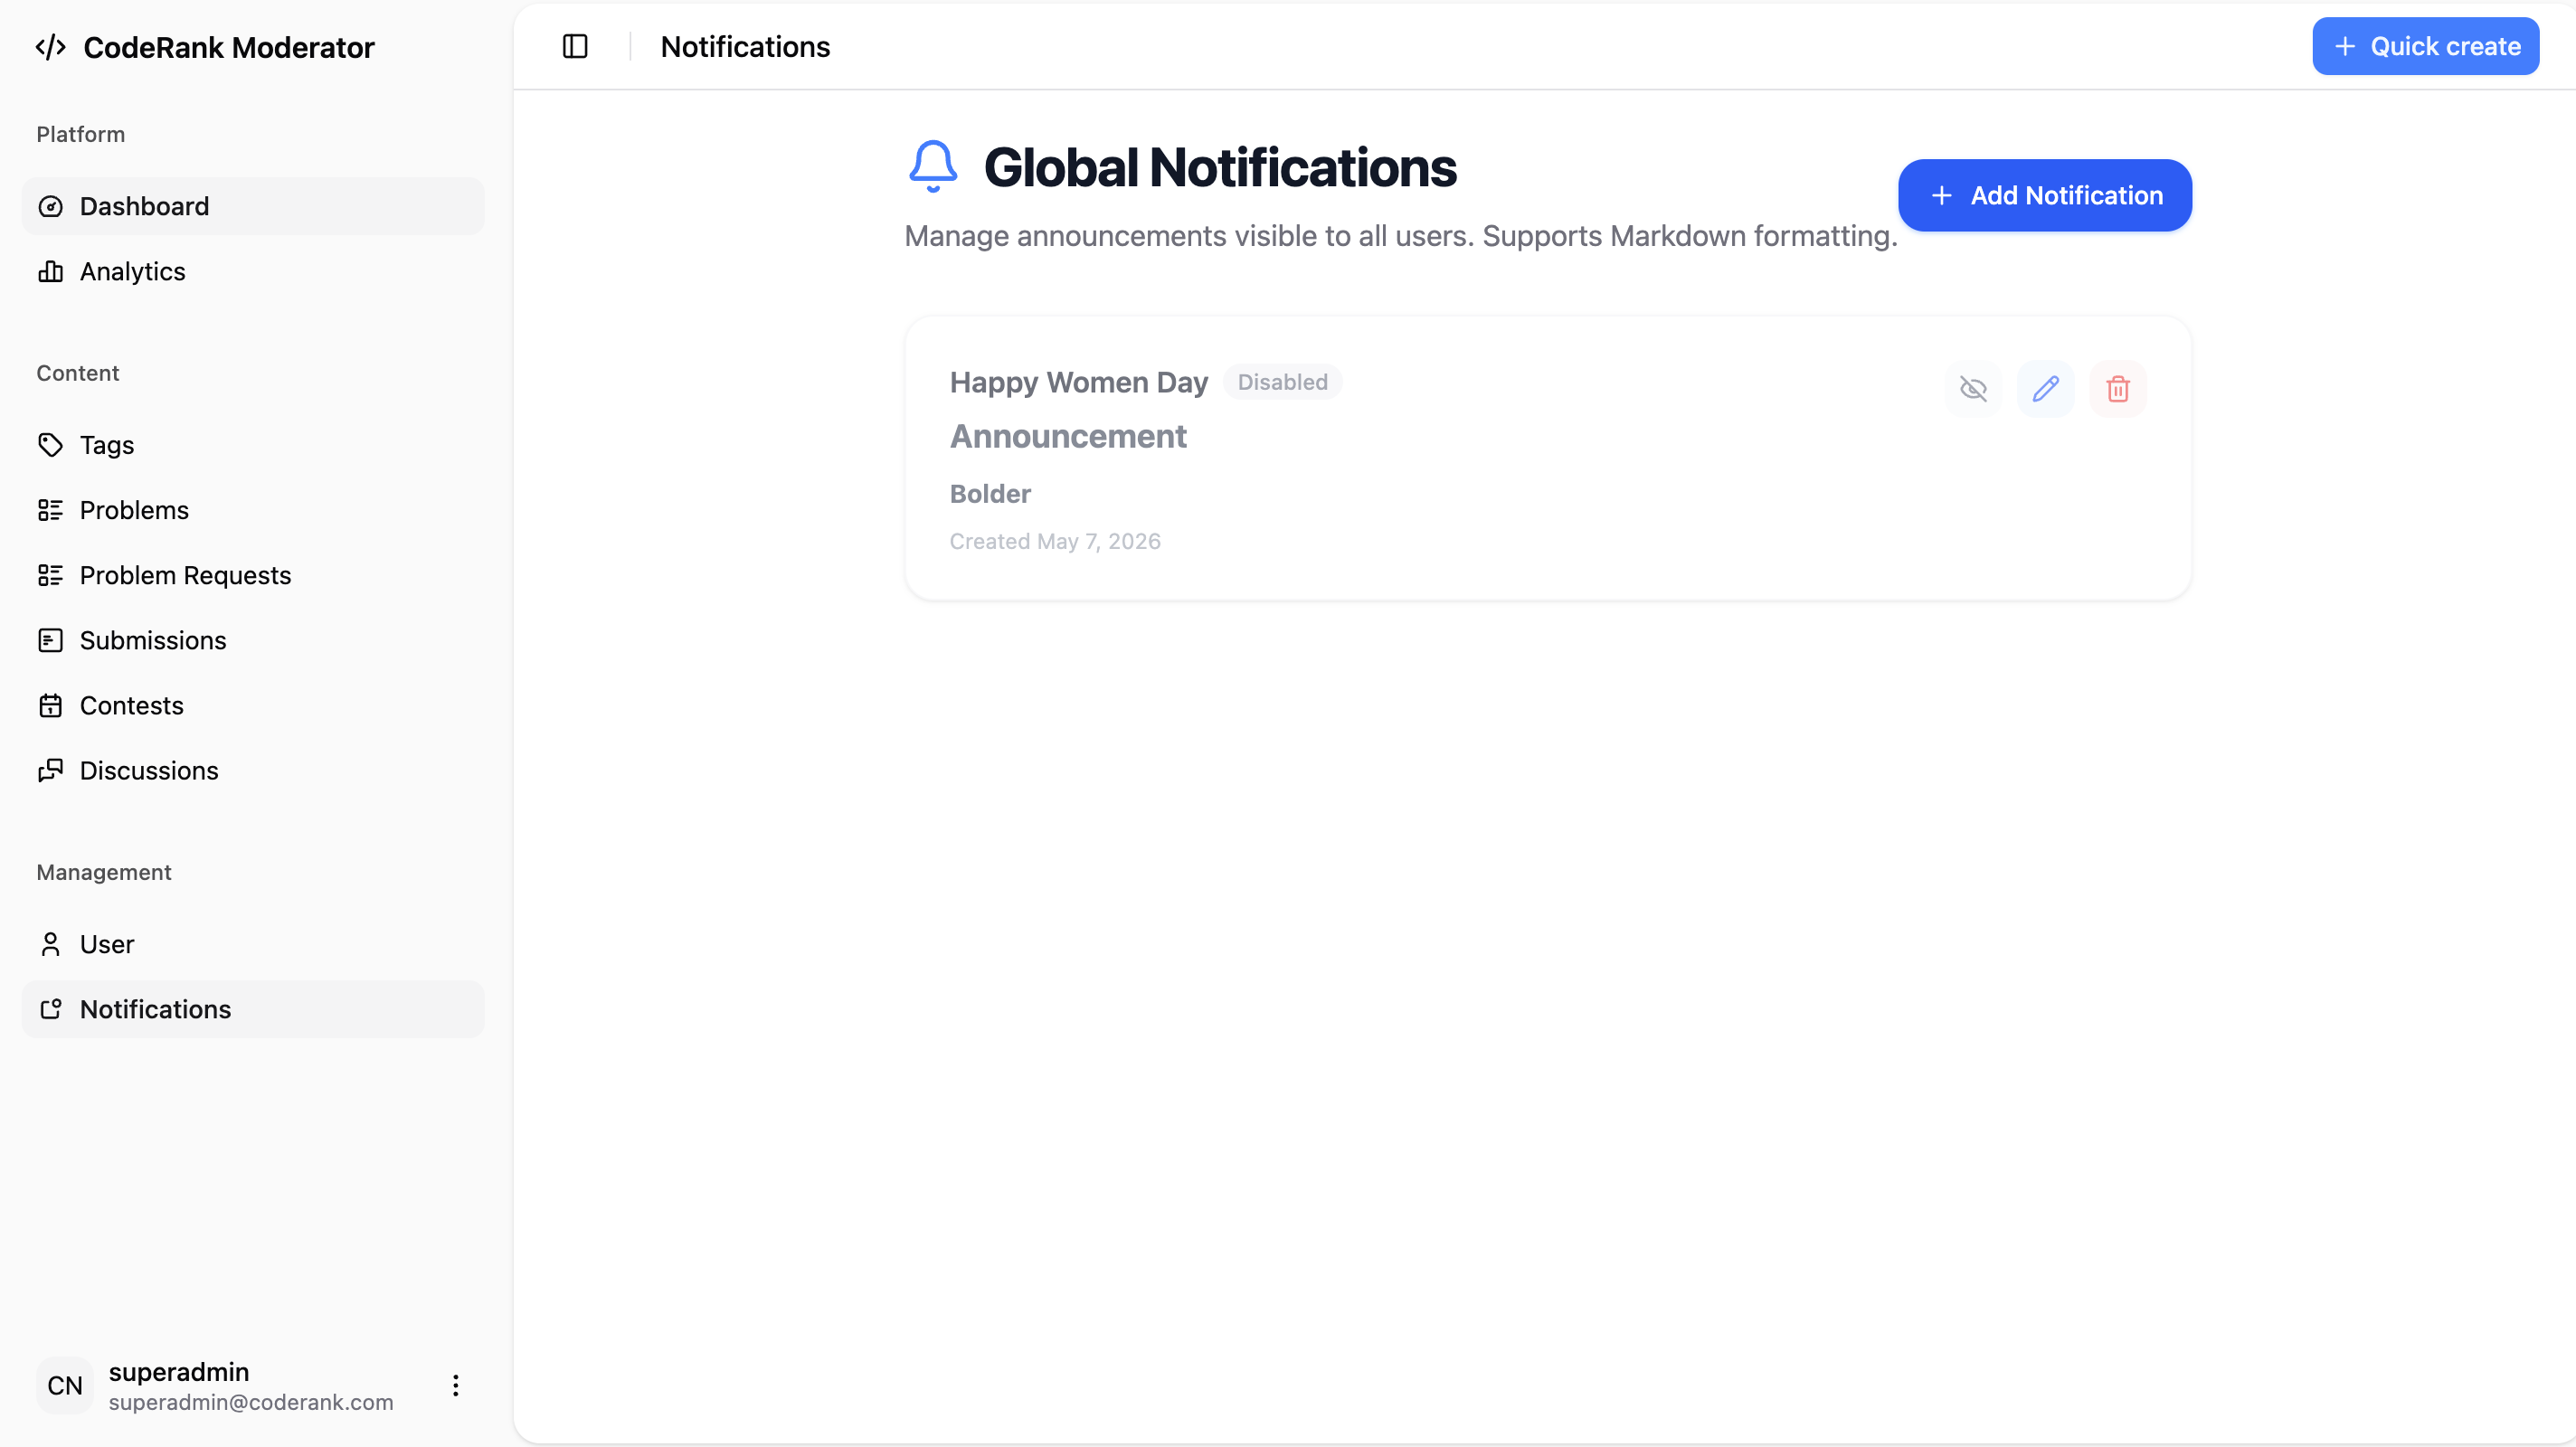
\includegraphics[width=1\textwidth]{Contents/Chapter 4/Mockup Design/Admin/notification_management.png}
    \vspace{0.6cm}
    \caption{Notification Management}
\end{figure}

Moderators/Admins can manage problem create requests submitted by another Moderator by navigating to the Problems sidebar, where a list of all problem requests is displayed along with their Difficulty level, color-coded for quick reference (Easy, Medium, Hard). In addition, this list is paginated, showing 10 items per page to ensure clear and efficient navigation.
\begin{figure}[H]
    \centering
    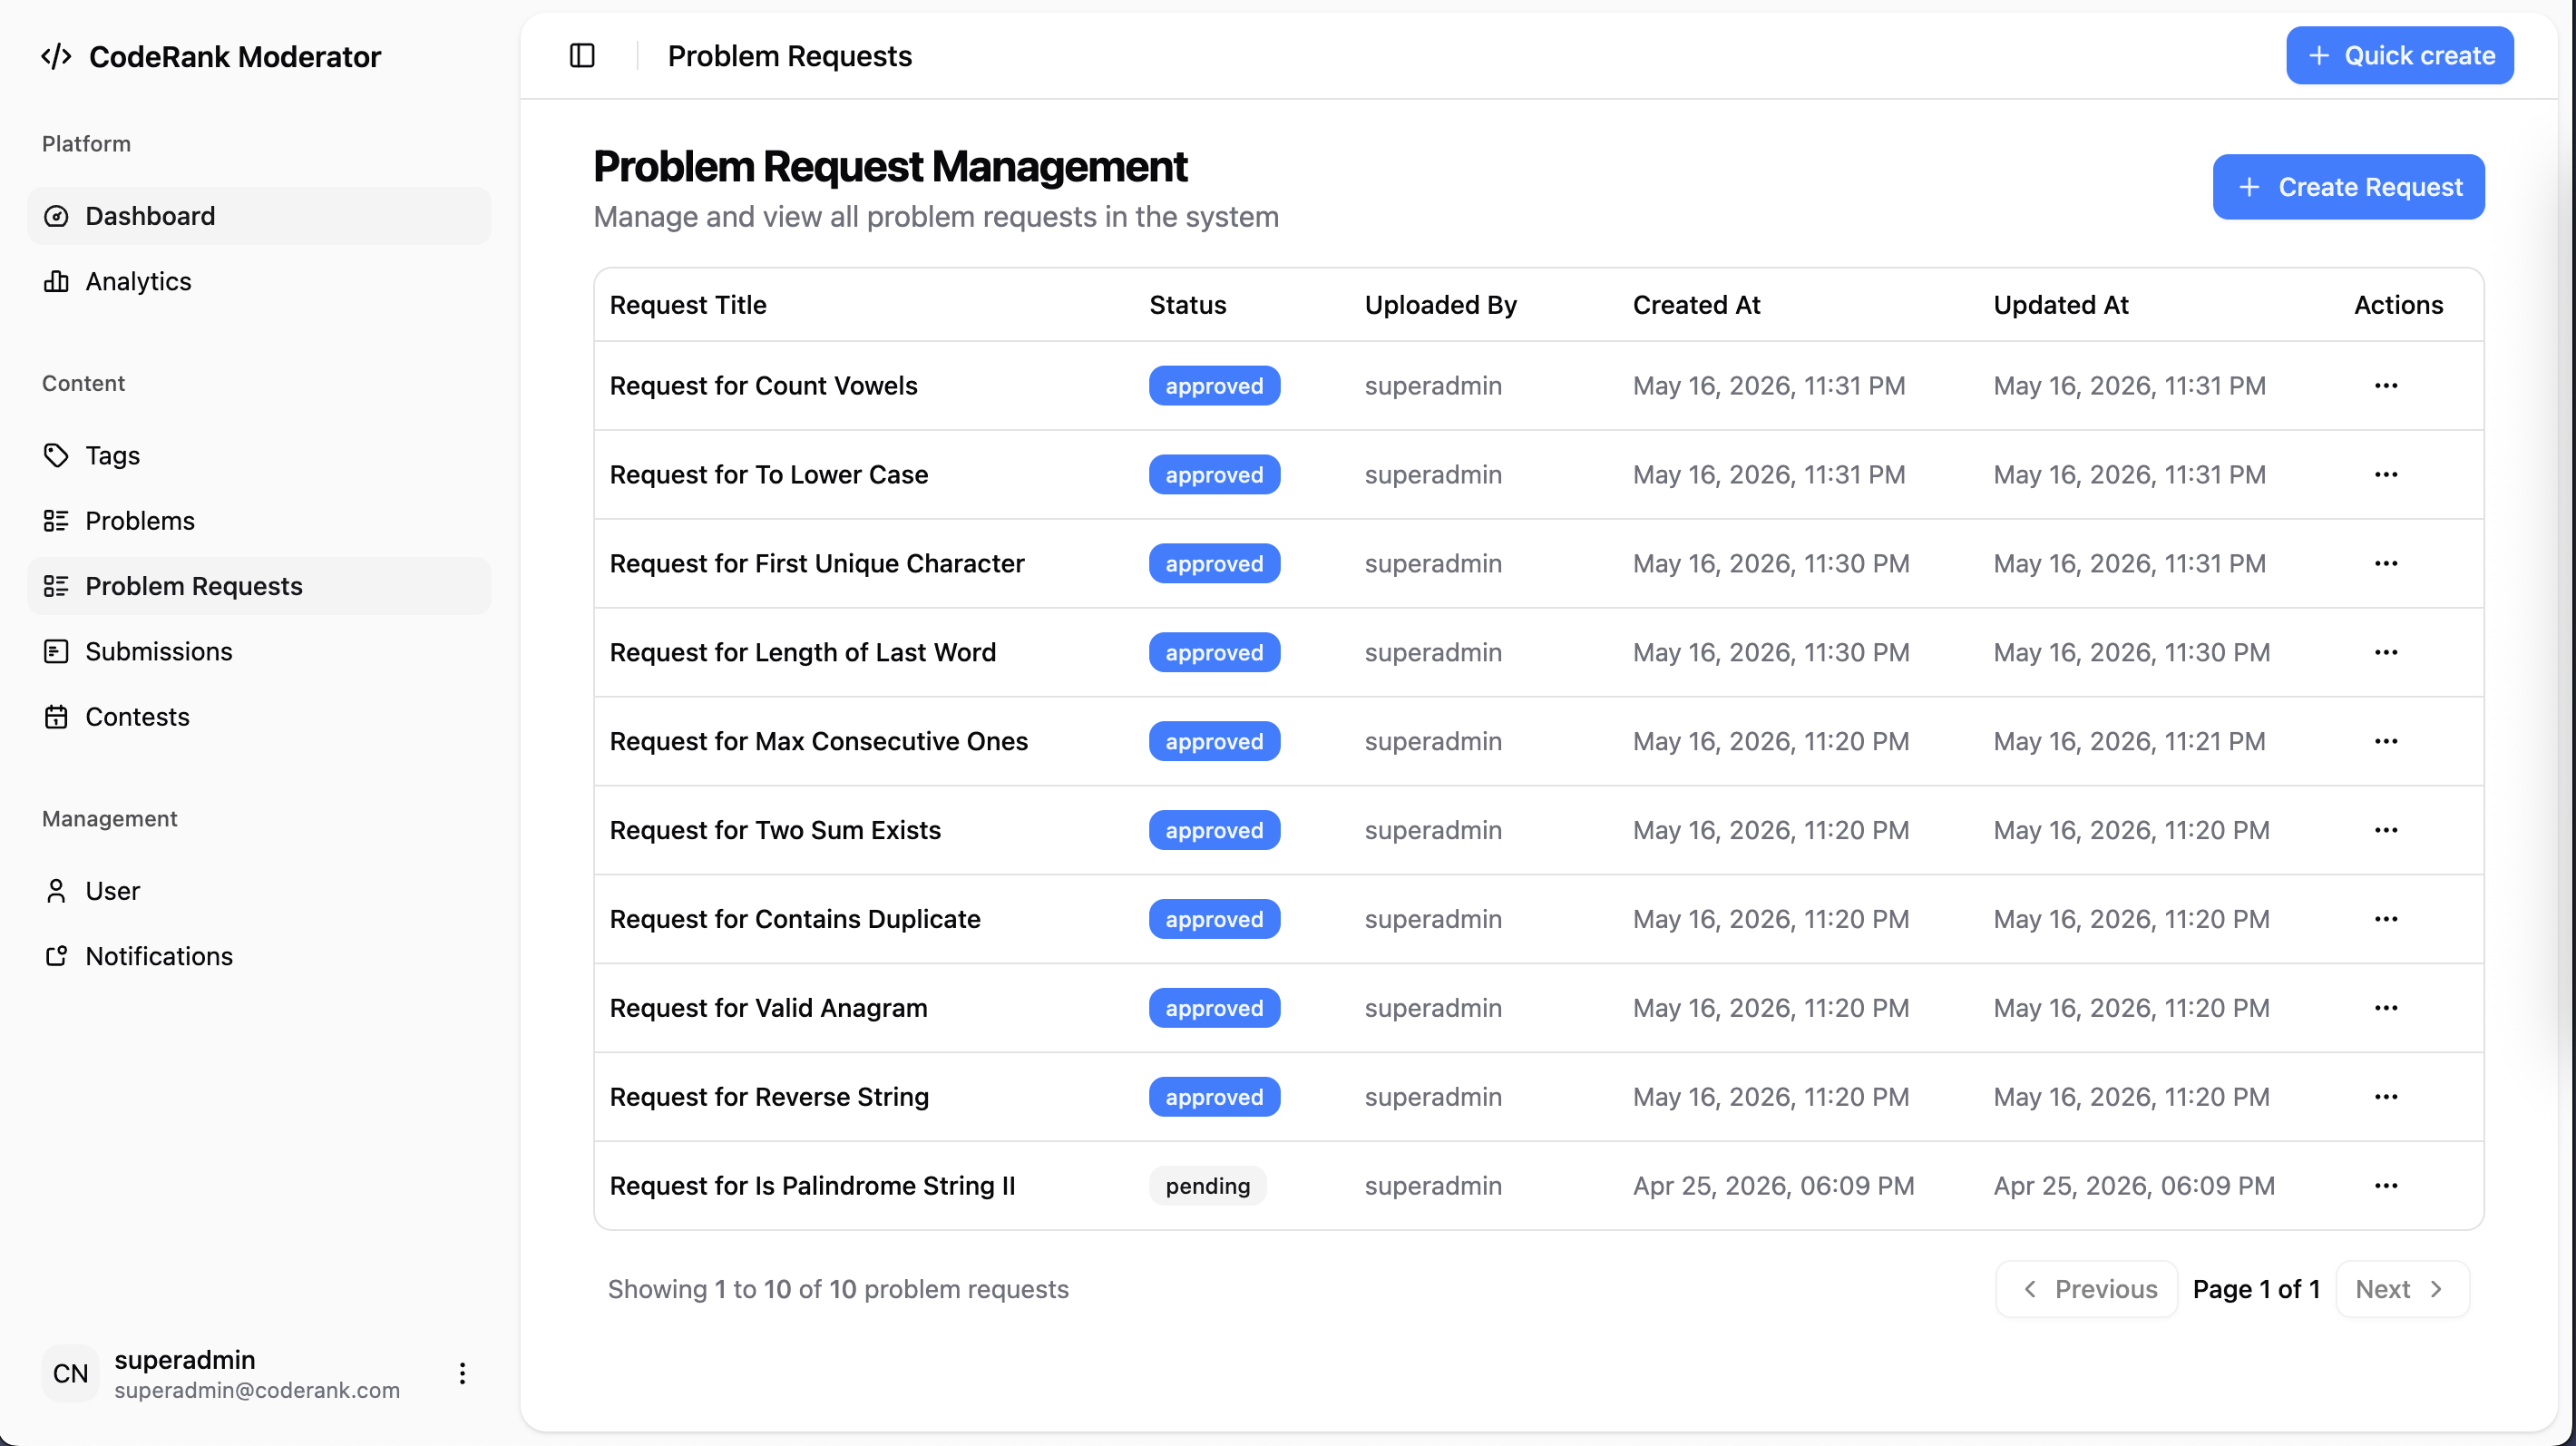
\includegraphics[width=1\textwidth]{Contents/Chapter 4/Mockup Design/Admin/Problem_request_list.png}
    \vspace{0.6cm}
    \caption{Problem Request List}
\end{figure}


A “Create Problem” button is positioned at the top-right corner of the interface, allowing users to quickly submit a new problem request. When this button is clicked, a creation modal appears centered on the screen, enabling Moderators/Admins to input all necessary details, in which user is required to fill in fields such as Problem Name, Difficulty level, Topic, and any other relevant information needed to define the problem.
\begin{figure}[H]
    \centering
    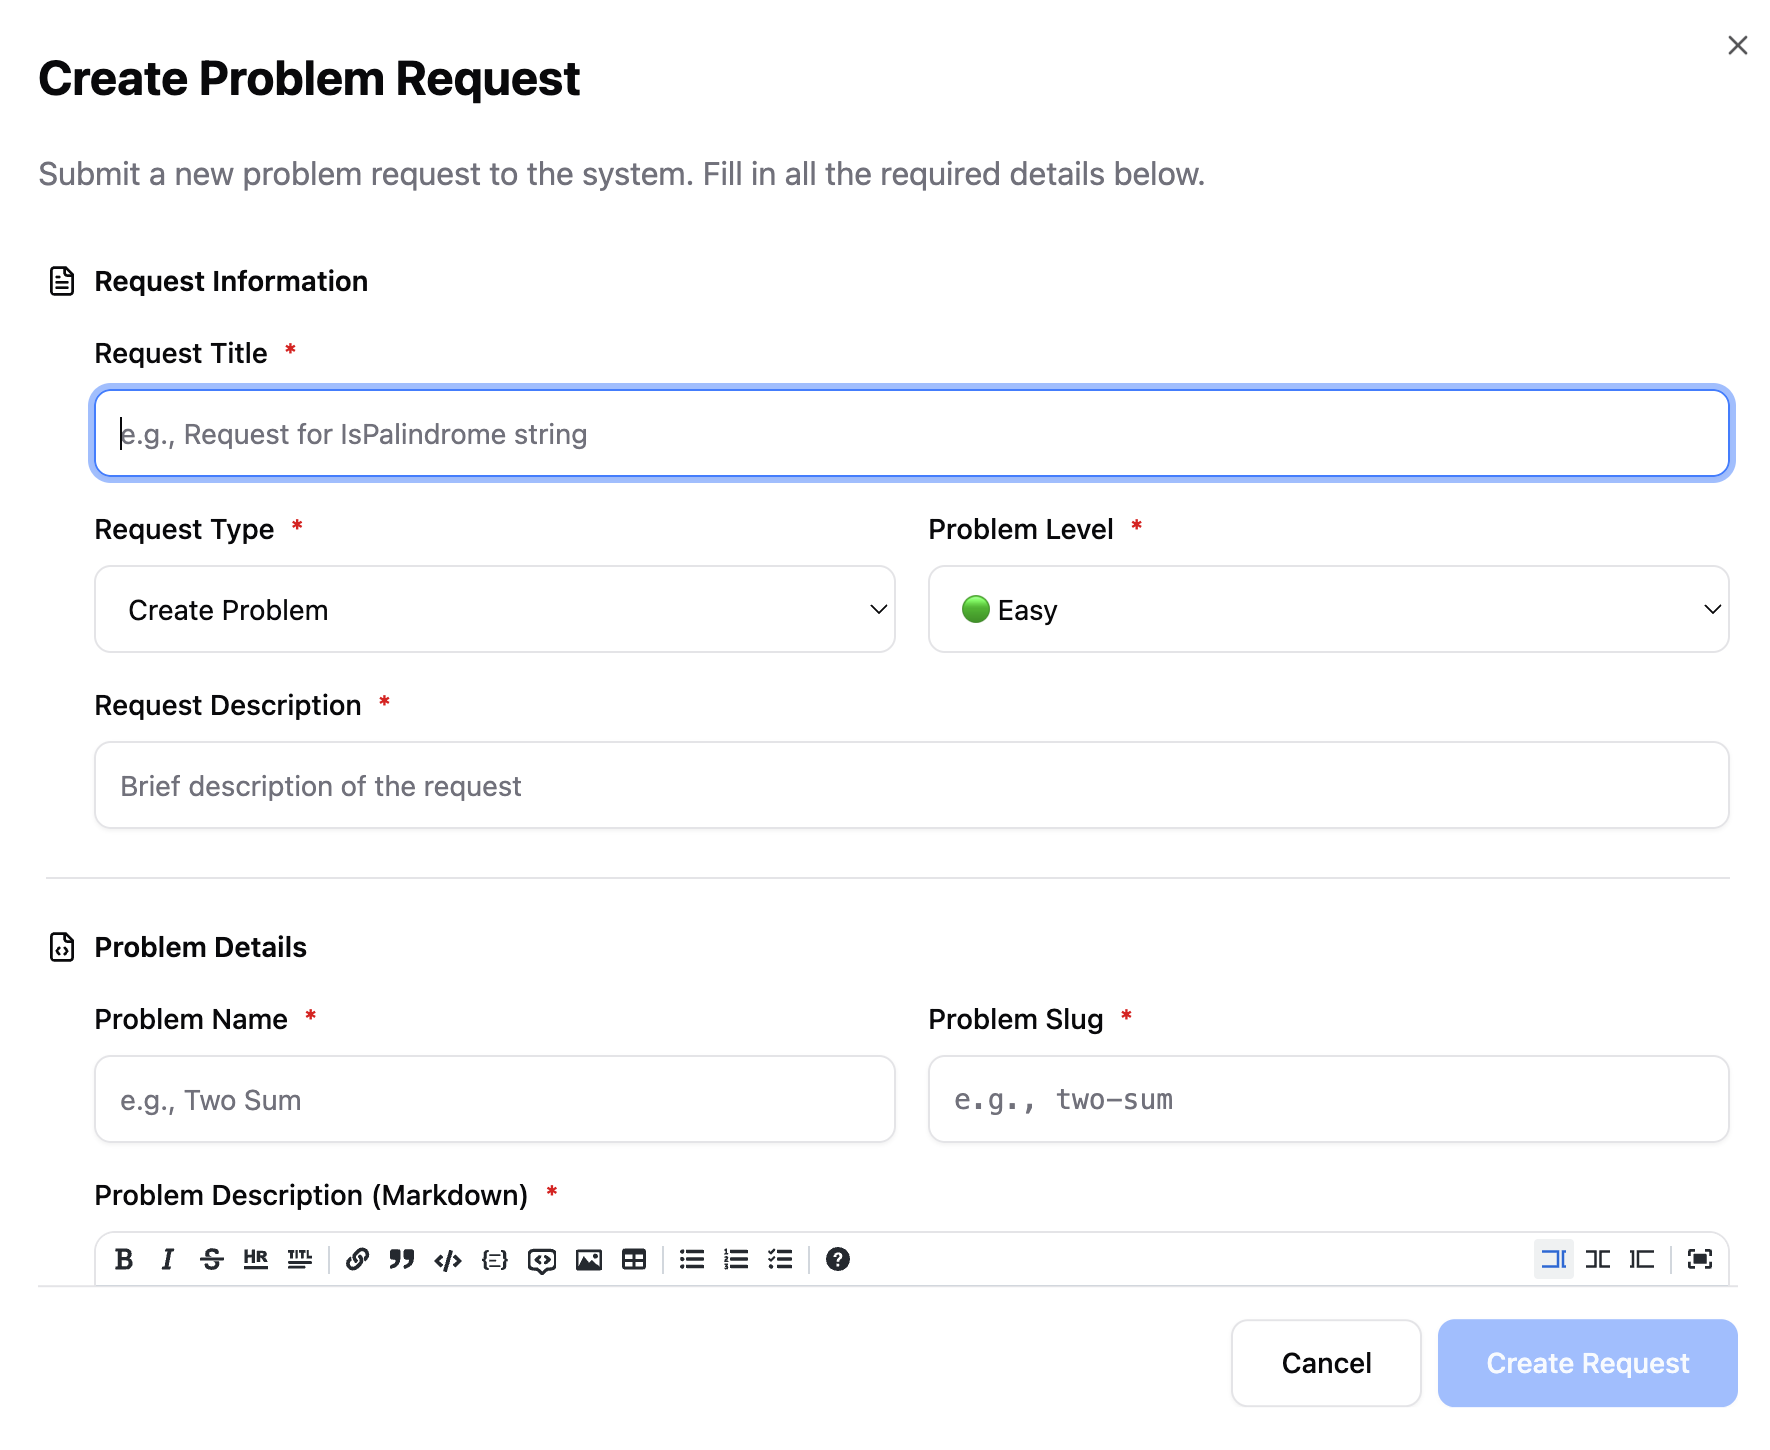
\includegraphics[width=1\textwidth]{Contents/Chapter 4/Mockup Design/Admin/Problem_request_modal.png}
    \vspace{0.6cm}
    \caption{Problem Request Create Modal}
\end{figure}

Moderators can also monitor submissions in real-time by navigating to the Submissions sidebar. This page displays a list of all submissions made by users, along with relevant details such as submission ID, user name, problem name, status (e.g., Accepted, Wrong Answer, Time Limit Exceeded), and submission time. Moderators can filter and sort the submissions based on various criteria to quickly identify any issues or patterns in user submissions.
\begin{figure}[H]
    \centering
    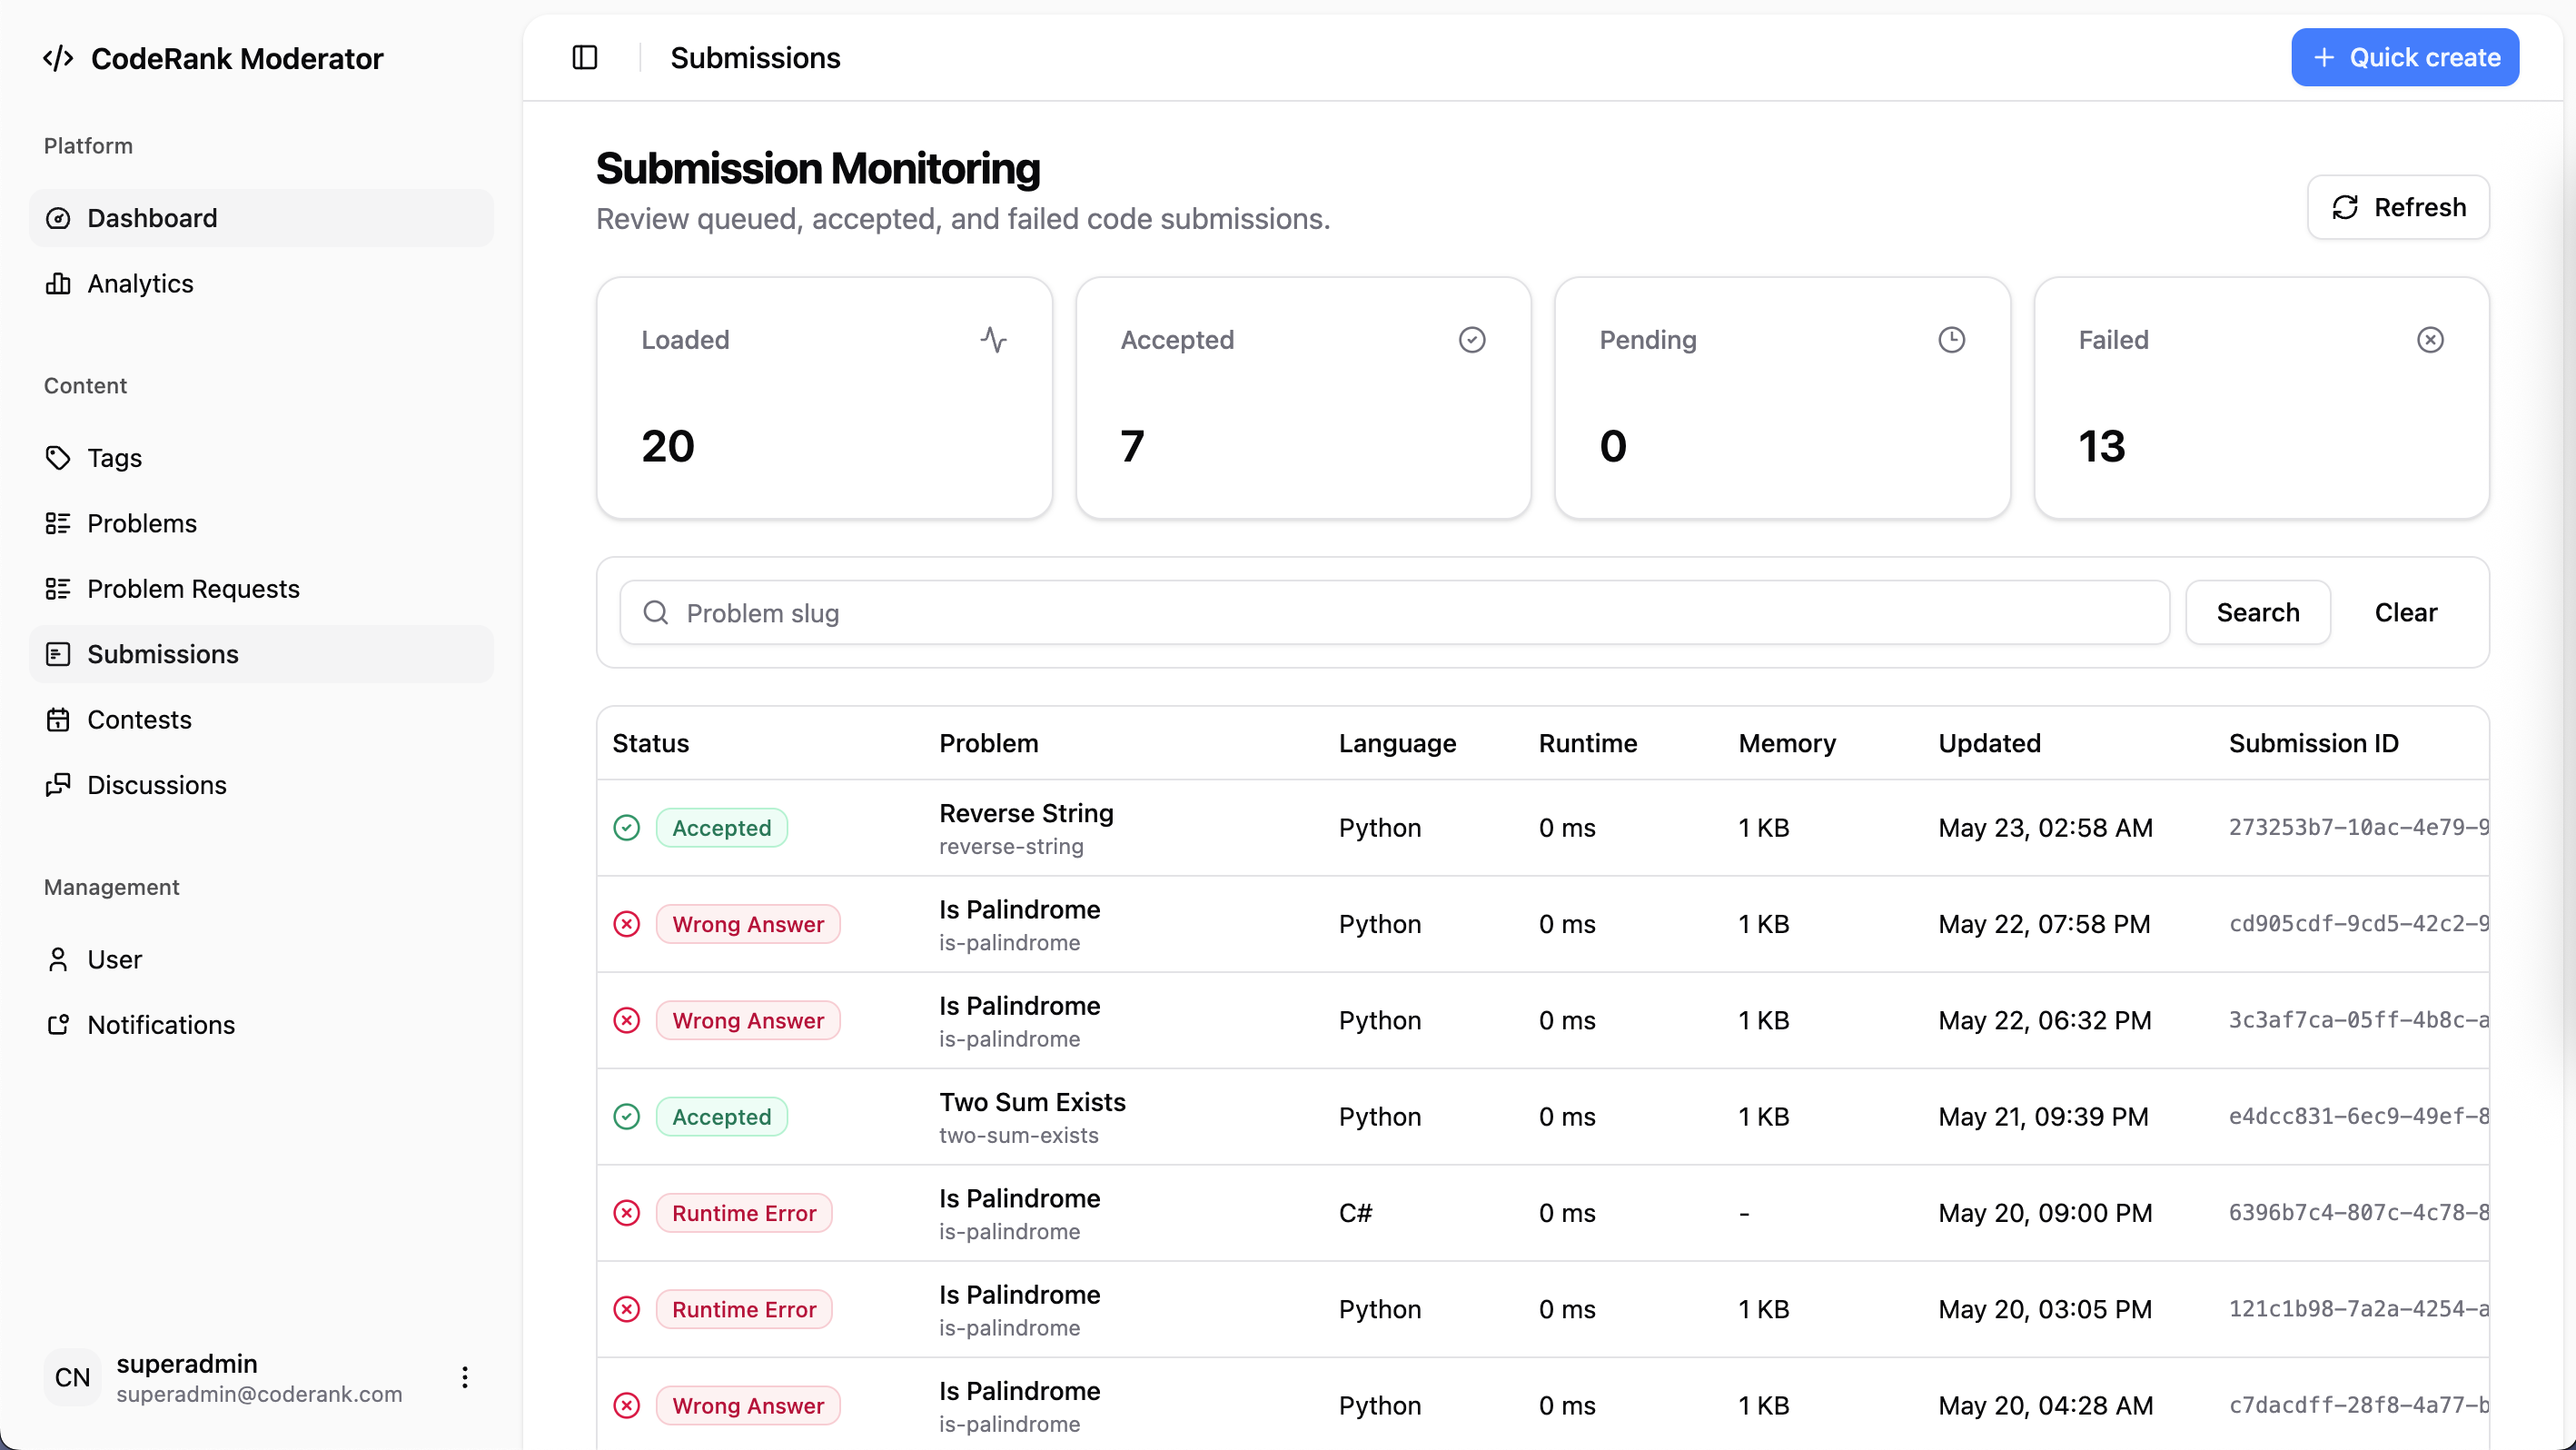
\includegraphics[width=1\textwidth]{Contents/Chapter 4/Mockup Design/Admin/submission_monitor.png}
    \vspace{0.6cm}
    \caption{Submission Monitor}
\end{figure}

Beside submissions, moderators can also monitor current discussions by navigating to the Discussions sidebar. This page displays a list of all active discussion threads, along with relevant details such as thread title, topic, number of messages, and last activity time. Moderators can filter and sort the discussions based on various criteria to quickly identify any issues or patterns in user discussions.
\begin{figure}[H]
    \centering
    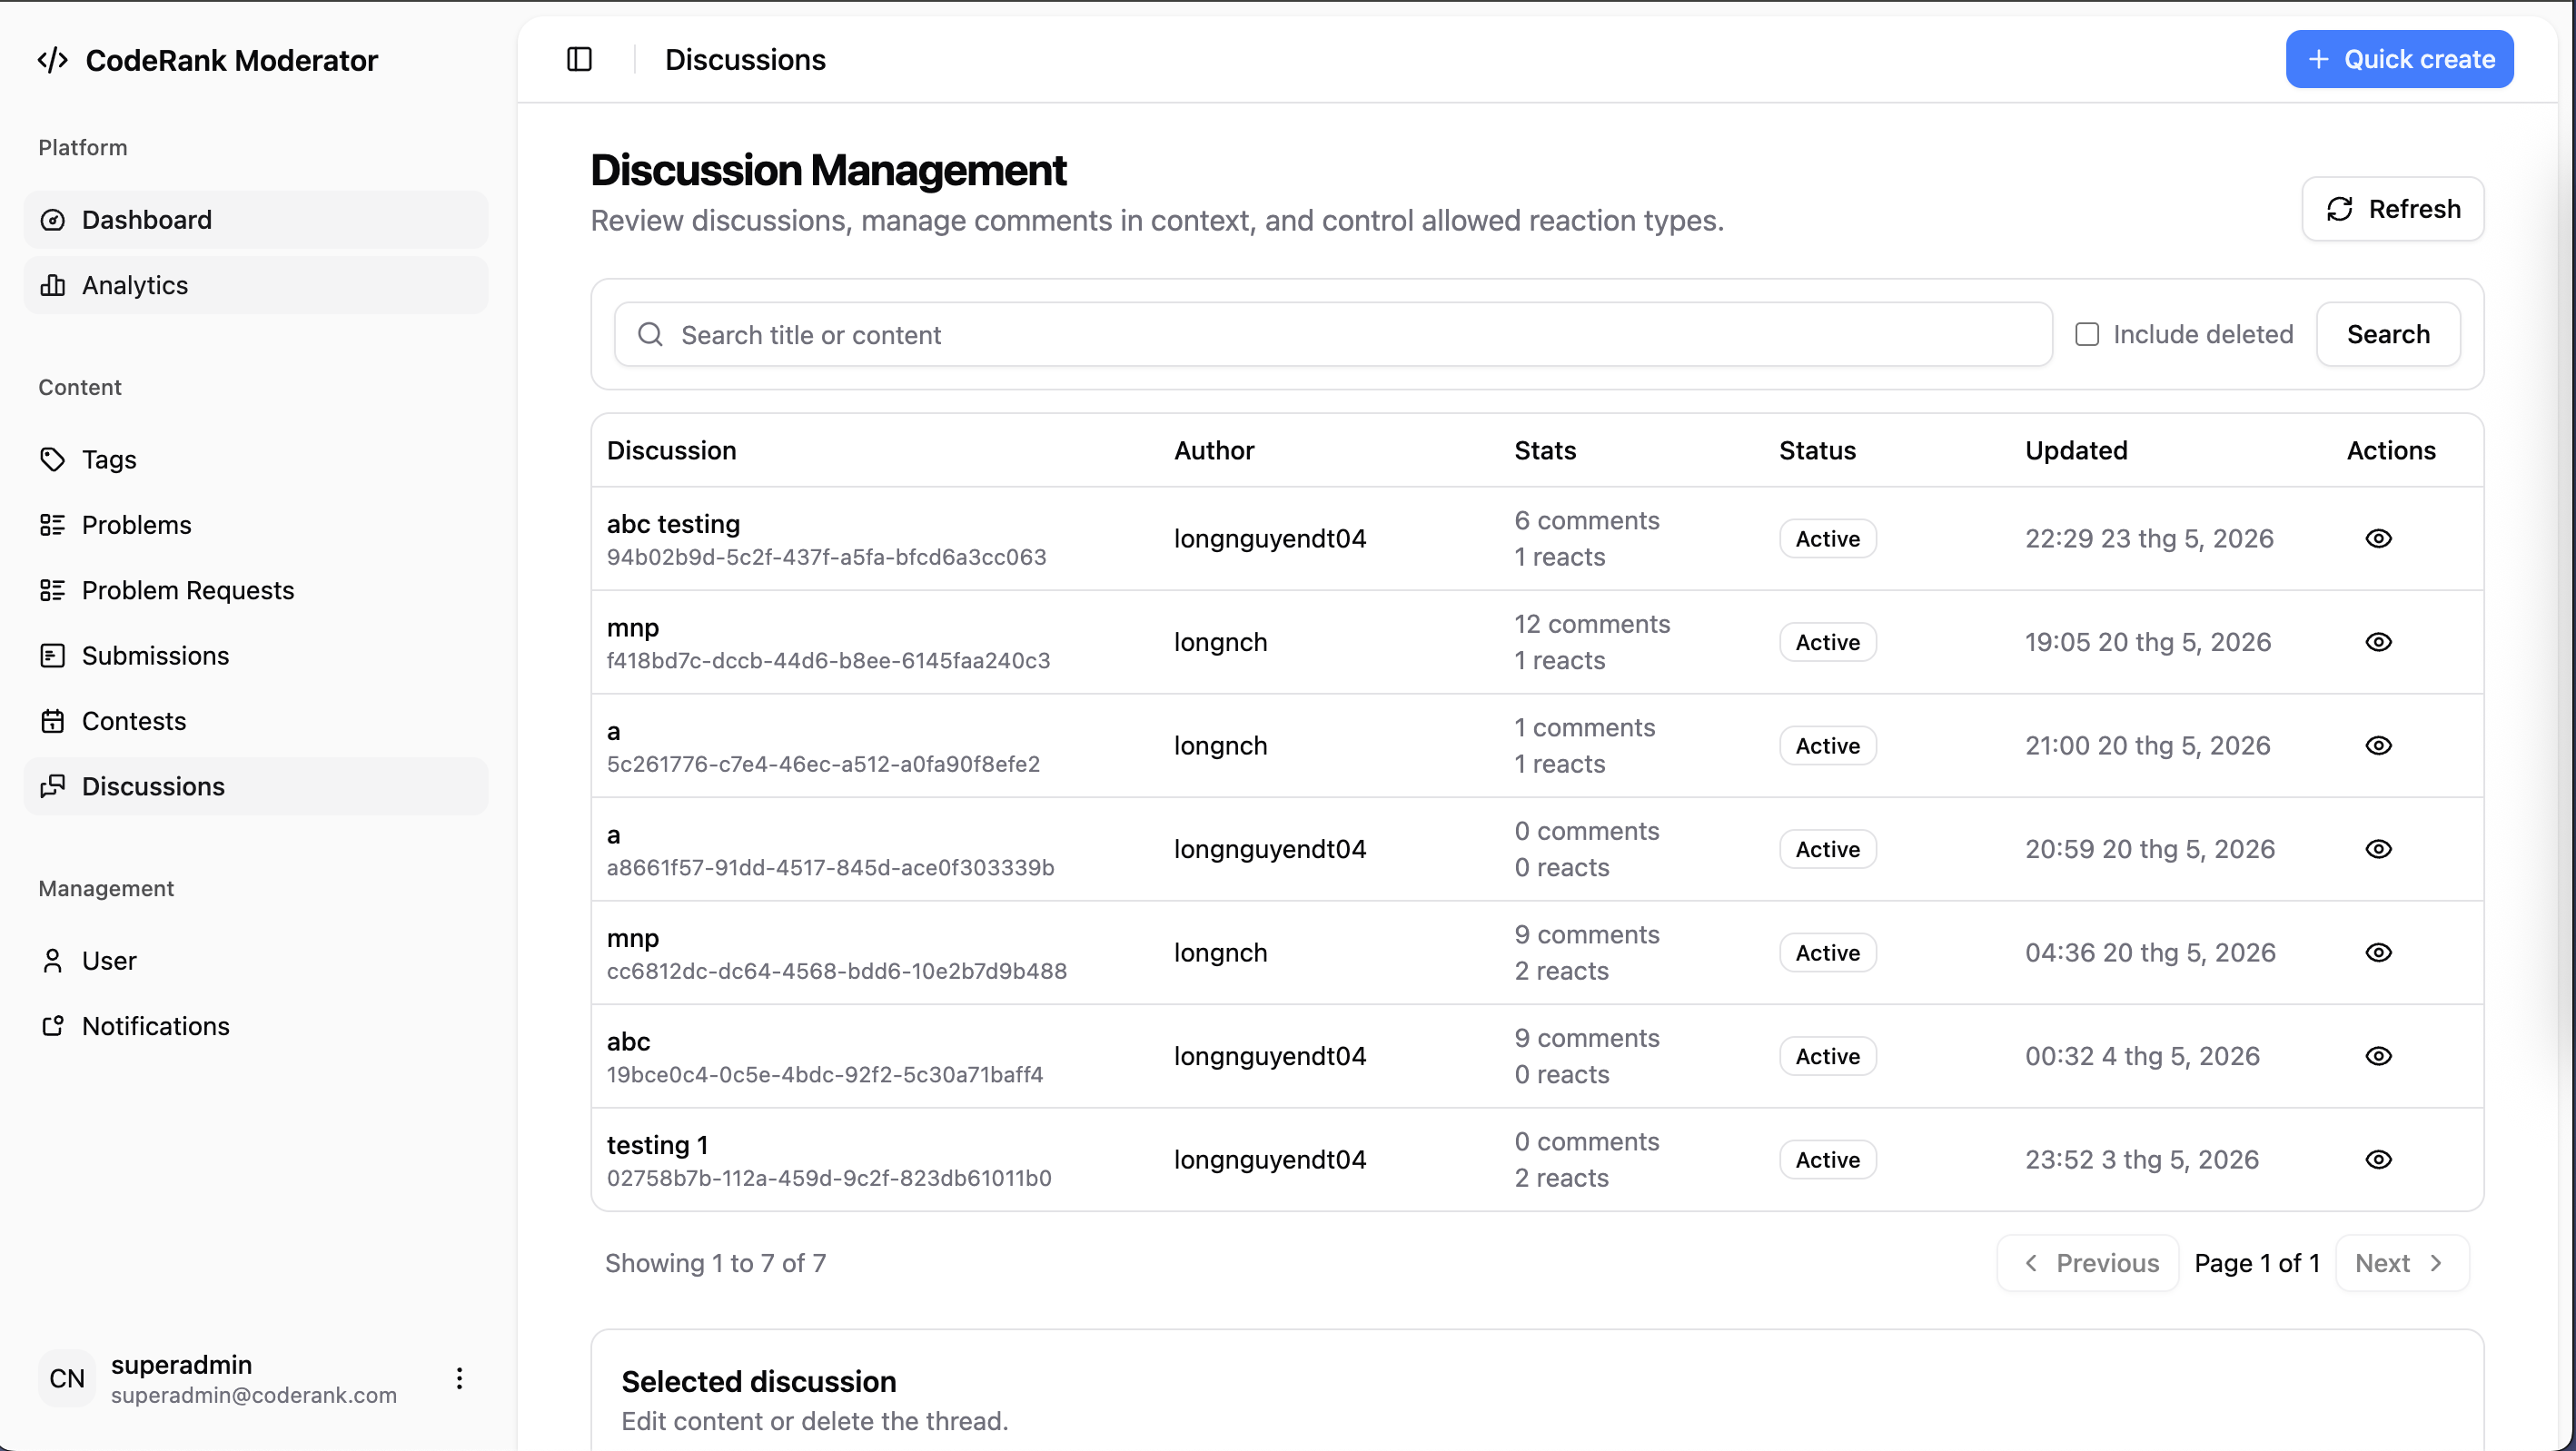
\includegraphics[width=1\textwidth]{Contents/Chapter 4/Mockup Design/Admin/discussion_monitor.png}
    \vspace{0.6cm}
    \caption{Discussion Monitor}
\end{figure}

Moderator can also managing notifications and announcements to all users by navigating to the Notifications sidebar. This page displays a list of all notifications sent to users, along with relevant details such as notification type, recipient user name, content summary, and timestamp. Moderators can filter and sort the notifications based on various criteria to quickly identify any issues or patterns in user notifications.
\begin{figure}[H]
    \centering
    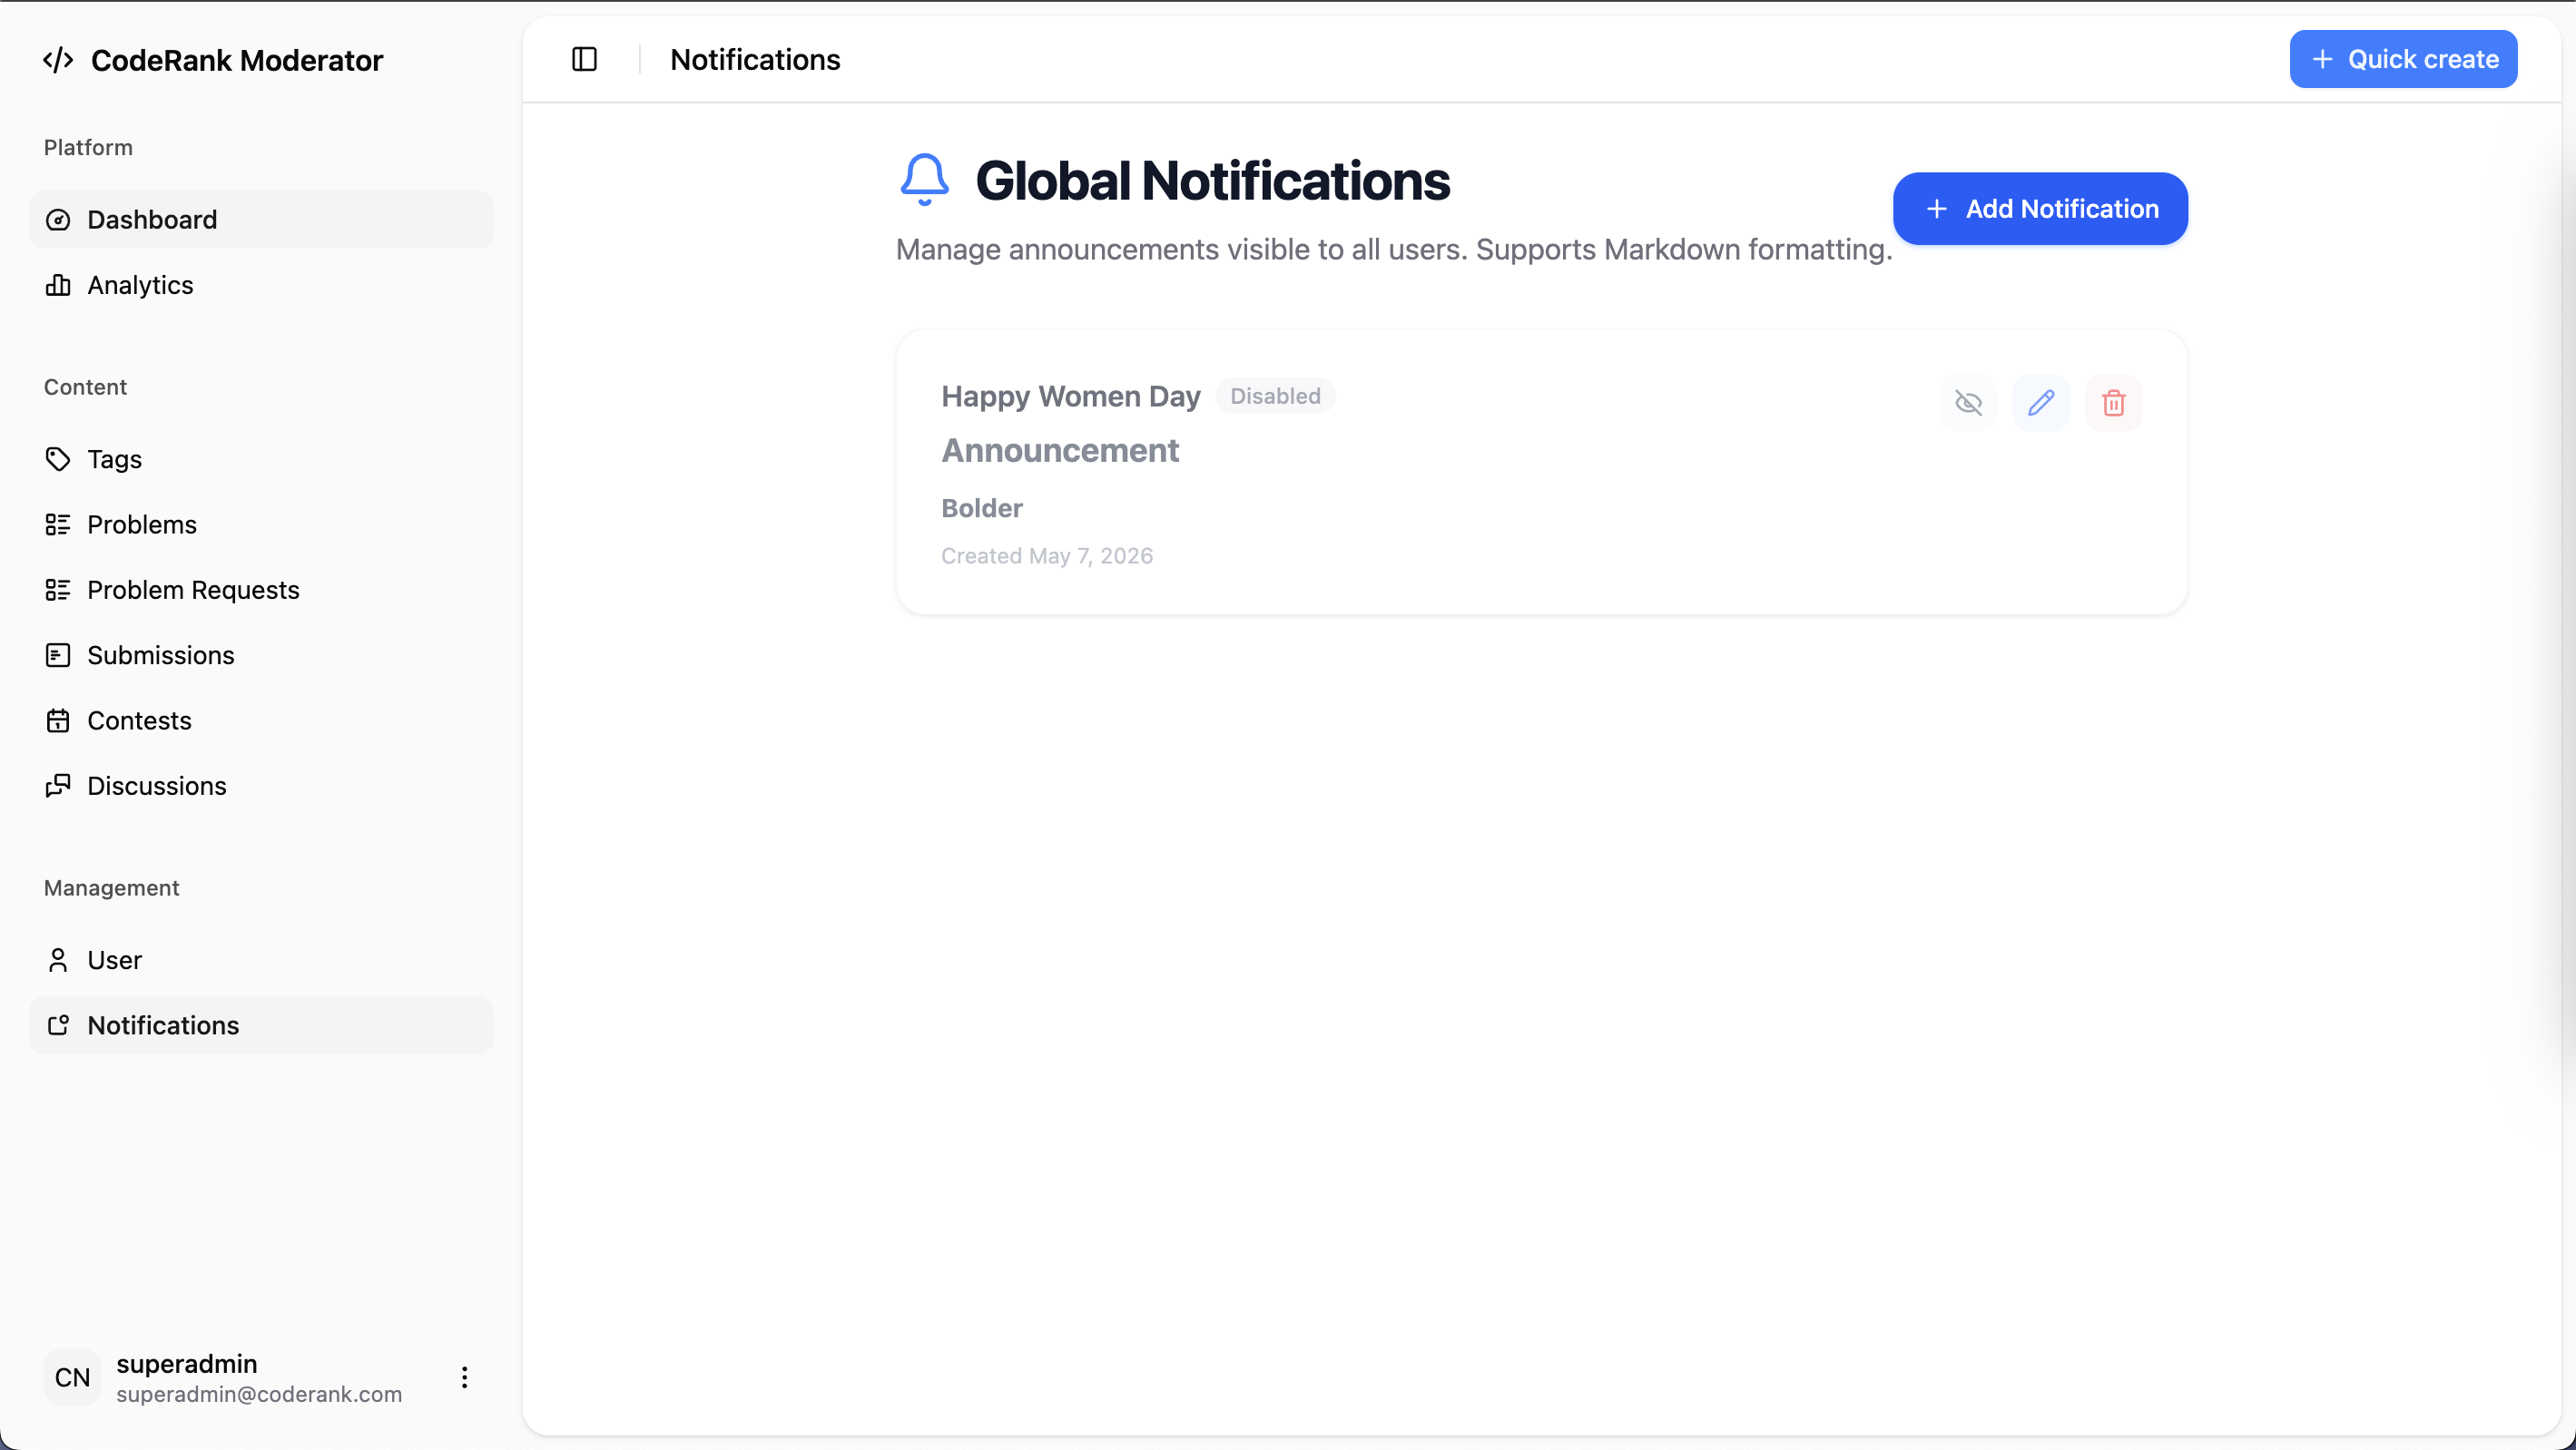
\includegraphics[width=1\textwidth]{Contents/Chapter 4/Mockup Design/Admin/app_notification.png}
    \vspace{0.6cm}
    \caption{Notification Setting}
\end{figure}

% \section{Chatbot Implementation}

This section describes the detailed implementation of the chatbot subsystem in the CodeRank system. The implementation focuses on enabling real-time, streaming-based conversational interaction between the user and the AI assistant.

The chatbot is implemented using a multi-layer architecture consisting of the frontend client, backend API server, n8n workflow engine, and Gemini large language model. A key feature of the system is the use of Server-Sent Events (SSE) to support streaming responses, providing a real-time chat experience similar to modern AI assistants.

\subsection{End-to-End Chatbot Request Flow}

When a user interacts with the chatbot, the system processes the request through the following sequence:

\begin{enumerate}
    \item The user submits a message from the frontend chatbot interface.
    
    \item The frontend immediately sends the message to the backend API server using an HTTP request.
    
    \item The backend receives the request and initiates a processing pipeline by calling an internal chatbot service.
    
    \item The backend triggers an n8n workflow via a webhook, passing the user input and conversation metadata.
    
    \item n8n processes the request and communicates with the Gemini model to generate a response.
    
    \item The response is streamed back from n8n to the backend.
    
    \item The backend forwards the streamed response to the frontend using Server-Sent Events (SSE).
    
    \item The frontend renders the response incrementally in real time as tokens are received.
\end{enumerate}

This architecture ensures low-latency interaction and improves user experience by allowing the response to appear progressively instead of waiting for the full output.

\subsection{Backend Processing and Streaming Architecture}

The backend plays a critical role in managing request orchestration and enabling real-time response streaming.

After receiving the request from the frontend, the backend does not wait for the full response from the AI pipeline. Instead, it establishes a Server-Sent Events (SSE) connection with the client and acts as a streaming proxy between n8n and the frontend.

The backend performs the following tasks:

\begin{itemize}
    \item Validates incoming chatbot requests
    \item Forwards the request to the n8n webhook endpoint
    \item Receives streamed response chunks from n8n
    \item Forwards each chunk to the frontend via SSE channel
\end{itemize}

This streaming mechanism allows the system to handle long AI-generated responses efficiently while maintaining responsiveness.

\subsection{n8n Workflow Execution and Streaming Response}

Within the n8n workflow, the chatbot request is processed through multiple stages including context retrieval, prompt construction, and LLM inference.

Unlike traditional synchronous APIs, the integration is designed to support incremental response generation. As the Gemini model produces output, n8n streams partial results back to the backend instead of waiting for the full completion.

This streaming behavior is essential for enabling real-time chat experiences and reducing perceived latency.

The workflow acts as an intermediate layer that:
\begin{itemize}
    \item Receives user input from the backend via webhook
    \item Processes conversational context and memory
    \item Sends structured prompts to the Gemini model
    \item Streams generated tokens or response chunks back to the backend
\end{itemize}

\subsection{Frontend Streaming with Server-Sent Events (SSE)}

On the frontend side, the chatbot interface establishes a persistent SSE connection with the backend.

When a user sends a message, the frontend immediately displays a loading state and begins listening for streamed response events.

As the backend receives chunks of data from n8n, it forwards them to the frontend incrementally. The frontend then appends each received chunk to the chat interface in real time.

This results in a typewriter-like effect where the response appears progressively, significantly improving user experience compared to traditional request-response models.

The SSE-based approach provides the following benefits:
\begin{itemize}
    \item Low latency response rendering
    \item Improved perceived system performance
    \item Smooth real-time interaction experience
    \item Reduced waiting time for long AI outputs
\end{itemize}


% \input{Outro/TaiLieuThamKhao}
% \newpage
% \input{Outro/PhuLuc}

\endgroup
\bibliographystyle{unsrt}
\bibliography{refs}

\newpage
\vspace{2cm}

\renewcommand{\thesection}{A}

\section*{A}

% \addcontentsline{toc}{section}{\protect\numberline{A}Appendix: Task Assignment}
\doublespacing

\noindent \textbf{\Huge Appendix: Task Assignment} 

\noindent\rule{\textwidth}{0.4pt}

\noindent
\textbf{Nguyen Chau Hoang Long }
\begin{itemize}
    \item Related work and comparison
    \item Requirement analysis
    \item Stakeholders description
    \item Technology Stack Front-end, Back-end, Database
    \item Use case diagram: Authentication \& Authorization, Contest, Discussion
    \item Use case description table
    \item Architecture Design
    \item Database Design
    \item Moderator/Admin wireframe design
\end{itemize}

\noindent
\textbf{Cao Ngoc Lam }
\begin{itemize}
    \item Requirement analysis
    \item Stakeholders description
    \item Technology Sandboxed Execution Environment, Artificial Intelligence
    \item Use case diagram:  System Management, Submission, Interview Practice
    \item Use case description table
    \item Chatbot implementation and design 
    \item Architecture Design
    \item Database Design
    \item Code Runner
    \item Primary User wireframe design
\end{itemize}


\end{document}